\documentclass[12pt,oneside]{book}
\usepackage[a4paper, margin=1in, headheight=15pt]{geometry}
\usepackage{setspace}
\usepackage{graphicx}
\usepackage[export]{adjustbox}
\usepackage{titlesec}
\usepackage{array}
\usepackage{enumitem}
\usepackage{multirow}
\usepackage{booktabs}
\usepackage{longtable}
\usepackage{tabularx}
\usepackage{float}
\usepackage{url}
\usepackage{rotating}
\usepackage{fancyhdr}
\usepackage{needspace}
\renewcommand{\arraystretch}{1.2}
\renewcommand{\bibname}{References}
% Words that must not be split at a line end.
\hyphenation{plagiarism}

\setlength{\intextsep}{5pt}
% Long-table captions may use the full text width (no hyphenated wraps).
\setlength{\LTcapwidth}{\textwidth}
% Contents lists: a wider page-number column, so a title that fills the
% line still keeps a gap before its page number.
\makeatletter
\renewcommand{\@pnumwidth}{2.2em}
\renewcommand{\@tocrmarg}{3.2em}
\makeatother

\makeatletter
\def\@makechapterhead#1{%
  {\parindent \z@ \raggedright \normalfont
    \ifnum \c@secnumdepth >\m@ne
        \huge\bfseries \@chapapp\space \thechapter
        \par\nobreak
        \vskip 10\p@
    \fi
    \interlinepenalty\@M
    \Huge \bfseries #1\par\nobreak
    \vskip 10\p@
  }}
\def\@makeschapterhead#1{%
  {\parindent \z@ \raggedright
    \normalfont
    \interlinepenalty\@M
    \Huge \bfseries  #1\par\nobreak
    \vskip 10\p@
  }}
\makeatother

\titlespacing\section{0pt}{12pt plus 4pt minus 2pt}{6pt plus 2pt minus 2pt}
\titlespacing\subsection{0pt}{10pt plus 3pt minus 2pt}{4pt plus 2pt minus 1pt}
\titlespacing\subsubsection{0pt}{8pt plus 2pt minus 2pt}{0.5em}

\titleformat{\subsubsection}[runin]
  {\normalfont\normalsize\bfseries}{\thesubsubsection}{1em}{}[.]

\newcommand\tab[1][0.75cm]{\hspace*{#1}}
\setcounter{tocdepth}{2}
\setcounter{secnumdepth}{3}

\newcommand{\hiddensubsection}[1]{
    \stepcounter{subsection}
    \subsection*{\arabic{chapter}.\arabic{section}.\arabic{subsection}\hspace{1em}{#1}}
}

\newcommand{\hiddensection}[1]{
    \stepcounter{subsection}
    \subsection*{\arabic{chapter}.\arabic{section}\hspace{1em}{#1}}
}

\newcolumntype{C}[1]{>{\centering\arraybackslash}m{#1}}
\newcolumntype{P}[1]{>{\raggedright\arraybackslash}p{#1}}

\usepackage{amssymb}
\usepackage{pifont}
\newcommand{\cmark}{\ding{51}}%
\newcommand{\xmark}{\ding{55}}%

% \DiagramBarrier, a local copy of the placeins \FloatBarrier (the package is
% not loaded), flushes pending figures before the next paragraph, so each
% paragraph in Chapters 5 and 6 is followed by its own figures.
\makeatletter
\newcommand{\DiagramBarrier}{\par\begingroup\let\@elt\relax
  \edef\@tempa{\@botlist\@deferlist\@dbldeferlist}%
  \ifx\@tempa\@empty\else\clearpage\fi\endgroup}
% \SoftBarrier flushes waiting figures only when the current page is already
% well filled, so a figure stays close to its paragraph without leaving a
% near-empty text page: one waiting figure at 75% of the page, two at 40%,
% three or more at 20%.
\newcount\sb@n \newcount\sb@s
\def\sb@count#1{\global\advance\sb@n\@ne
  \ifdim\ht#1<0.6\textheight\global\advance\sb@s\@ne\fi}
\def\sb@a{0.75}\def\sb@b{0.4}\def\sb@c{0.2}
% The flush is \newpage when at most one small figure waits (it then goes to
% the top of the next page, beside text) and \clearpage otherwise.
\def\sb@flush{\ifnum\sb@s>\@ne\clearpage\else\newpage\fi}
\newcommand{\SoftBarrier}{\par\begingroup
  \global\sb@n\z@ \global\sb@s\z@ \let\@elt\sb@count \@deferlist
  \ifdim\pagegoal=\maxdimen \dimen@\z@ \else \dimen@\pagetotal \fi
  \@tempswafalse
  \ifnum\sb@n>\z@  \ifdim\dimen@>\sb@a\pagegoal \@tempswatrue\fi\fi
  \ifnum\sb@n>\@ne \ifdim\dimen@>\sb@b\pagegoal \@tempswatrue\fi\fi
  \ifnum\sb@n>\tw@ \ifdim\dimen@>\sb@c\pagegoal \@tempswatrue\fi\fi
  \if@tempswa\aftergroup\sb@flush\fi\endgroup}
% \SoftBarrierN (Chapter 6 screenshots) only ends the page (\newpage), so a
% screenshot too small for a page of its own waits for the top of the next
% page instead of standing alone; its limits are 60%, 30% and 15%.
\newcommand{\SoftBarrierN}{{\let\sb@flush\newpage
  \def\sb@a{0.6}\def\sb@b{0.3}\def\sb@c{0.15}\SoftBarrier}}
% Each diagram in Chapters 4 and 5 is printed right after its short explanation
% (at most two printed lines, checked on the PDF whenever a text is edited).
% \DiagramFig{size}{file}{caption}{label}{text} starts a new page first when the
% text, the diagram and its caption would not fit on the rest of the page, so the
% text and its diagram always stay together. Diagram sizes keep the smallest
% printed text at 6.5 pt or more.
\newsavebox{\dg@box}
\newcommand{\DiagramFig}[5]{%
  \sbox{\dg@box}{\includegraphics[#1]{Figures/#2}}%
  \par\begingroup
    \dimen@=\ht\dg@box \advance\dimen@ by 7\baselineskip
    \dimen@ii=\pagegoal \advance\dimen@ii by -\pagetotal
    % When the page is already over full, TeX breaks it before this point by
    % itself, so only a page with room left is checked.
    \ifdim\pagegoal<\maxdimen \ifdim\dimen@ii>\z@
      \ifdim\dimen@>\dimen@ii \aftergroup\newpage\fi\fi\fi
  \endgroup
  #5\par
  \begin{figure}[H]
  \centering
  \usebox{\dg@box}
  \caption{#3}
  \label{#4}
  \end{figure}}
\makeatother

\begin{document}

% Front matter: roman numbers at the bottom centre. The title, certificate
% and declaration pages are counted but print no number.
\pagenumbering{roman}
\pagestyle{plain}
\thispagestyle{empty}
\onehalfspacing

\begin{center}
\vspace*{12pt}

\includegraphics[width=2in]{Figures/Logo.jpg}

\vspace{1cm}

{\Huge\textbf{AI-Driven Lab Exam Monitoring\\
and Management System}\par}

\vspace{5cm}

\normalsize
\textbf{Zain Ali Mehmood (2280133)}\\
\textbf{Muhammad Haider Ali (2280354)}\\
\textbf{Roshaan Ali Shah (2280327)}

\vspace{2cm}

\textbf{Supervised by: Ms.~Zainab Iftikhar Chaudhary}

\vspace*{\fill}
\textbf{In partial fulfillment of the requirements for the degree}\\
\textbf{Bachelor of Science (Software Engineering)}\\
\textbf{Shaheed Zulfikar Ali Bhutto Institute of Science and Technology}\\
\textbf{Islamabad, Pakistan}

\vspace{10pt}
\textbf{Spring, 2026}
\end{center}

\singlespacing
\newpage
\thispagestyle{empty}

\begin{center}
\vspace*{0.8cm}

{\bfseries\fontsize{20}{24}\selectfont 
AI-Driven Lab Exam Monitoring and\\
Management System\par}

\vspace{0.8cm}

{\bfseries\itshape\fontsize{16}{18}\selectfont By\par}

\vspace{0.5cm}

{\bfseries\itshape\fontsize{14}{16}\selectfont
Zain Ali Mehmood (2280133)\\
Muhammad Haider Ali (2280354)\\
Roshaan Ali Shah (2280327)\par}

\vspace{0.8cm}

{\bfseries\fontsize{22}{26}\selectfont CERTIFICATE\par}

\end{center}

\vspace{0.6cm}

\begin{center}
{\bfseries\fontsize{11}{14}\selectfont
A THESIS SUBMITTED IN PARTIAL FULFILLMENT OF THE REQUIREMENTS FOR THE DEGREE OF BACHELOR OF SCIENCE IN SOFTWARE ENGINEERING (BSSE).\par}
\end{center}

\vspace{2.5cm}

\noindent
\begin{minipage}{0.48\textwidth}
\centering
\rule{6cm}{0.4pt}\\[4pt]
(Supervisor)\\
Ms. Zainab Iftikhar Chaudhary
\end{minipage}
\hfill
\begin{minipage}{0.48\textwidth}
\centering
\rule{6cm}{0.4pt}\\[4pt]
(FYP Committee Head)\\
Mr. Ghaffar Ahmed
\end{minipage}

\vspace{1.5cm}

\begin{center}
\begin{minipage}{0.48\textwidth}
\centering
\rule{6cm}{0.4pt}\\[4pt]
(Program Manager BSSE)\\
Mr. Sheikh Abdul Wahab
\end{minipage}
\end{center}

\vspace{1cm}

\begin{center}
Date: \rule{4.5cm}{0.4pt}
\end{center}

\vfill

\begin{center}
\normalsize\textbf{Department of Computer Science, Shaheed Zulfikar Ali Bhutto Institute of Science and Technology, Islamabad Campus}\\
\vspace{6pt}
\normalsize\textbf{Fall, 2026}
\end{center}
\newpage
\thispagestyle{empty}
\begin{center}
    {\Huge\textbf{DECLARATION}}
\end{center}
\vspace{1cm}

\begin{onehalfspacing}
We, Zain Ali Mehmood (2280133), Muhammad Haider Ali (2280354) and Roshaan Ali Shah (2280327), students of the Bachelor of Science in Software Engineering at Shaheed Zulfikar Ali Bhutto Institute of Science and Technology, Islamabad, declare that the project titled ``AI-Driven Lab Exam Monitoring and Management System'' is our own work.

This project has not been submitted before for any degree or examination at any other university or institute. We have acknowledged all sources of information and data used in this document.\par
\end{onehalfspacing}

\vspace{2cm}

\noindent
\begin{minipage}{0.45\textwidth}
\centering
\rule{6cm}{0.4pt}\\[4pt]
Zain Ali Mehmood\\
(2280133)
\end{minipage}
\hfill
\begin{minipage}{0.45\textwidth}
\centering
\rule{6cm}{0.4pt}\\[4pt]
Muhammad Haider Ali\\
(2280354)
\end{minipage}

\vspace{1.8cm}

\begin{center}
\begin{minipage}{0.45\textwidth}
\centering
\rule{6cm}{0.4pt}\\[4pt]
Roshaan Ali Shah\\
(2280327)
\end{minipage}
\end{center}

\newpage
\thispagestyle{empty}
\chapter*{\centering Project Overview}
\addcontentsline{toc}{chapter}{Project Overview}

A practical lab exam is hard to supervise. One or two invigilators watch 30 to 40 screens, attendance is marked on paper, and code is collected on USB drives. SmartExam, the system built for our registered project ``AI-Driven Lab Exam Monitoring and Management System'', replaces this with three parts: a Windows Presentation Foundation (WPF) client on each lab PC, a React web panel for staff and students, and an ASP.NET Core 9 API backed by PostgreSQL on Neon.

Teachers create exams with multiple-choice (MCQ), coding and theory questions, set eligibility from imported attendance and assign each student a workstation. A student can log in only from the workstation bound to the account by its hardware ID. After a readiness check, the client locks the PC: fullscreen window, blocked shortcuts, clipboard guard and a check for unapproved programs. It reports heartbeats, focus and process events, screenshots and, when the exam requires it, webcam checks (camera covered or frozen, no face or several faces, head turned away, phone in view); no face is matched to an identity. A rule-based classifier rates each student, and invigilators follow every seat on a live dashboard, from which they can warn a student, extend time, unlock the PC or force a submission. Each edit goes to an encrypted local backup within a second and to the server within 10 seconds. Practice exams let students rehearse without affecting their results.

After each submission, C and C++ answers run against the teacher's test cases in an isolated Docker container where available (otherwise with a local compiler that is not isolated), theory answers get a TF-IDF similarity score, and a plagiarism check flags similar code. The teacher reviews every suggested mark. Security-relevant actions are kept in a hash-chained, tamper-evident audit log, and teachers export PDF reports, an Excel workbook and an evidence ZIP. We built the system in eight four-week Agile sprints. Automated unit, integration, API and browser tests cover all twelve modules (Chapter~7); checks that need a real lab PC, such as the webcam, USB and 40-client load checks, are still pending.

\newpage
\thispagestyle{empty}
\chapter*{\centering Dedication}
\addcontentsline{toc}{chapter}{Dedication}
%\centerline{\textbf{\LARGE DEDICATION}}
\par\bigskip
Firstly, we dedicate this project to Allah Almighty, whose blessings, mercy, and guidance made this effort possible. We also dedicate this work to our Holy Prophet Muhammad (Peace Be Upon Him), whose teachings remain a source of inspiration in all aspects of life. Finally, we dedicate this project to our beloved parents, respected teachers, supervisor, and supportive friends whose prayers, encouragement, and sacrifices have helped us continue our academic journey with determination and hope.

\newpage
\thispagestyle{empty}

\chapter*{\centering Acknowledgements}
\addcontentsline{toc}{chapter}{Acknowledgements}
\par\bigskip
This Final Year Project has been completed in partial fulfillment of the requirements for the degree of Bachelor of Science in Software Engineering. We sincerely thank our supervisor, Ms. Zainab Iftikhar Chaudhary, for her guidance, encouragement, and constructive feedback throughout the development of this project. We are also grateful to the faculty members of the Department of Computer Science, SZABIST Islamabad, and our families and friends for their continuous support, motivation, and prayers during the planning, implementation, and report-writing phases of this work.

\vspace{2cm}

\noindent
\begin{minipage}{0.45\textwidth}
\centering
\rule{6cm}{0.4pt}\\[4pt]
Zain Ali Mehmood\\
(2280133)
\end{minipage}
\hfill
\begin{minipage}{0.45\textwidth}
\centering
\rule{6cm}{0.4pt}\\[4pt]
Muhammad Haider Ali\\
(2280354)
\end{minipage}

\vspace{1.8cm}

\begin{center}
\begin{minipage}{0.45\textwidth}
\centering
\rule{6cm}{0.4pt}\\[4pt]
Roshaan Ali Shah\\
(2280327)
\end{minipage}
\end{center}

\chapter*{Revision History}
\addcontentsline{toc}{chapter}{Revision History}

\begin{center}
\footnotesize
\setlength{\tabcolsep}{4pt}
\renewcommand{\arraystretch}{1.2}
\begin{tabularx}{\textwidth}{l l l >{\raggedright\arraybackslash}X l}
\hline\hline
\textbf{Compiled By} & \textbf{Checked By} & \textbf{Date} & \textbf{Reason for Change} & \textbf{Version} \\
\hline
All members & Ms. Zainab Iftikhar Chaudhary & 24 Feb 2026 & FYP-I proposal submitted & 0.1 \\
Muhammad Haider Ali & Ms. Zainab Iftikhar Chaudhary & 10 Mar 2026 & Chapter 1 drafted from the proposal & 1.0 \\
Roshaan Ali Shah & Ms. Zainab Iftikhar Chaudhary & 16 Mar 2026 & Objectives (Section 1.3) added & 1.1 \\
Zain Ali Mehmood & Ms. Zainab Iftikhar Chaudhary & 22 Mar 2026 & Intended users (Section 1.7) added & 1.2 \\
Muhammad Haider Ali & Ms. Zainab Iftikhar Chaudhary & 28 Mar 2026 & SRS introduction (Section 2.1) & 1.3 \\
Roshaan Ali Shah & Ms. Zainab Iftikhar Chaudhary & 04 Apr 2026 & Chapter 3 project plan drafted & 1.4 \\
Zain Ali Mehmood & Ms. Zainab Iftikhar Chaudhary & 10 Apr 2026 & Management plan (Section 3.2) & 1.5 \\
Muhammad Haider Ali & Ms. Zainab Iftikhar Chaudhary & 15 Apr 2026 & Chapters 1--3 reviewed and refined & 1.6 \\
All members & Ms. Zainab Iftikhar Chaudhary & 18 Jun 2026 & FYP-I report submitted & 1.7 \\
Roshaan Ali Shah & Ms. Zainab Iftikhar Chaudhary & 05 Oct 2026 & Chapter 4 matched to the code & 1.8 \\
Zain Ali Mehmood & Ms. Zainab Iftikhar Chaudhary & 10 Oct 2026 & Chapter 5 design diagrams revised & 1.9 \\
Muhammad Haider Ali & Ms. Zainab Iftikhar Chaudhary & 15 Oct 2026 & Chapter 6 UI and tables revised & 2.0 \\
Roshaan Ali Shah & Ms. Zainab Iftikhar Chaudhary & 20 Oct 2026 & Chapter 7 test plan drafted & 2.1 \\
Muhammad Haider Ali & Ms. Zainab Iftikhar Chaudhary & 21 Oct 2026 & Module 12 tests and test run & 2.2 \\
Muhammad Haider Ali & Ms. Zainab Iftikhar Chaudhary & 26 Oct 2026 & Full review; final test run & 2.3 \\
Muhammad Haider Ali & Ms. Zainab Iftikhar Chaudhary & 27 Oct 2026 & Template sections added & 2.4 \\
Muhammad Haider Ali & Ms. Zainab Iftikhar Chaudhary & 29 Oct 2026 & Supervisor comments: use cases, test tables and figure text revised & 2.5 \\
\hline\hline
\end{tabularx}
\end{center}

\tableofcontents

% \clearpage first, so that each entry records the page where its list starts.
\clearpage
\addcontentsline{toc}{chapter}{List of Figures}
\listoffigures

\clearpage
\addcontentsline{toc}{chapter}{List of Tables}
\listoftables


% Main matter: arabic numbers from 1, at the top right of every page.
\clearpage
\pagenumbering{arabic}
% Space between paragraphs from here on only, so the contents lists keep
% their tight spacing. Table and float cells reset it to zero.
\setlength{\parskip}{6pt plus 2pt minus 1pt}
\fancypagestyle{plain}{%
  \fancyhf{}%
  \fancyhead[R]{\thepage}%
  \renewcommand{\headrulewidth}{0pt}%
  \renewcommand{\footrulewidth}{0pt}}
\pagestyle{plain}
\chapter{INTRODUCTION}
\label{chap:introduction}

This chapter introduces SmartExam. It states the product's purpose and scope, reviews existing tools, and sets out our objectives, the problem we address and the solution we propose. It ends with the intended market and users and the process model we followed.

\section{Product Purpose}
\label{sec:productpurpose}

Computer science and software engineering students are tested in practical lab exams. They write, compile and debug code on a real machine, which a multiple-choice paper cannot assess. In many departments these exams are still run by hand. The schedule is shared on WhatsApp, attendance is marked on a paper sheet, and students hand in their code by email or on a USB drive when time runs out. During the exam one or two invigilators walk between 30 and 40 machines. They cannot see every screen, and when they suspect cheating there is little record to check afterwards.

SmartExam is the system name of our registered project, the AI-Driven Lab Exam Monitoring and Management System, and it brings these steps together. Administrators manage users, roles, departments, courses, labs and workstations from a web panel. Teachers create exams with multiple-choice (MCQ), coding and theory questions, add test cases and list the applications students may use. Students log in on the Windows Presentation Foundation (WPF) client, which only works on their registered workstation. After a readiness check, the client locks the PC to the exam. Invigilators follow each seat on a live dashboard that shows focus changes, running processes, screenshots and warnings. As each student submits, the server grades coding answers against the test cases, scores theory answers and checks for plagiarism. The teacher reviews the suggested marks and can override any of them, and generates reports when needed. Students see their results on a web portal once the exam has ended.

Our aim is to make lab exams fair, supervised and auditable without adding staff to the room.

\section{Product Scope}

SmartExam covers a lab exam from set-up to final report. We drew the scope boundary \cite[ch.~5]{pmbok6} around the institution's own lab: exams on Windows PCs on campus, not at home. The WPF client on each workstation and the React web panel both talk to an ASP.NET Core 9 API that stores data in PostgreSQL on Neon. The web dashboard gets live updates from the API, and the desktop client receives staff commands, such as a warning or extra time, with its next heartbeat (every 10 s). The work is split into twelve modules:

\begin{itemize}[noitemsep]
\item \textbf{M1 Authentication and Device Binding:} secure login, hashed passwords and workstation binding by hardware ID.
\item \textbf{M2 Pre-Exam Verification and Practice Exam:} network, clock, webcam and secure-mode checks, practice exams.
\item \textbf{M3 Student Exam Dashboard:} assigned exam with start countdown, readiness and eligibility status, student web portal.
\item \textbf{M4 Secure Exam Environment (lockdown):} fullscreen window, blocked shortcuts, clipboard guard, Report or Enforce mode for unapproved apps.
\item \textbf{M5 Live Monitoring Client Service:} 10~s heartbeats, batched events, randomised screenshots, on-PC webcam checks.
\item \textbf{M6 Submission and Backup:} autosave, encrypted local backup, offline queue, server-side deadline and receipt.
\item \textbf{M7 User and Role Management:} account management and CSV import, five roles, binding reset, departments and courses.
\item \textbf{M8 Exam Creation and Configuration:} MCQ, coding and theory questions, test cases, allowed apps and lockdown mode, exam notices.
\item \textbf{M9 Eligibility and Access Control:} attendance import, 75\% rule, audited overrides, seat assignment.
\item \textbf{M10 Live Proctoring Dashboard:} live tiles, warnings and extra time, unlock and force-submit, incidents.
\item \textbf{M11 AI-Assisted Evaluation:} test-case grading of C and C++, MCQ marking, TF-IDF theory scoring, plagiarism matrix.
\item \textbf{M12 Logs, Analytics and Audit Trail:} hash-chained audit log, analytics, PDF reports, Excel and evidence-ZIP exports.
\end{itemize}

\subsection{Existing System Description}
\label{sec:existingsystems}

The manual process is described in Section~\ref{sec:productpurpose}. Existing tools each solve one part of it. We reviewed ten of them. Each is summarised below with its main features and its limitations for an exam held in a campus lab, and Table~\ref{tab:comparison} compares all ten.

Table~\ref{tab:Abbreviations} lists, in alphabetical order, the abbreviations used in this report with their full forms.

\begin{longtable}{cl>{\raggedright\arraybackslash}p{9.6cm}}
\caption{Abbreviations}
\label{tab:Abbreviations}\\
\hline\hline
\textbf{Serial \#} & \textbf{Abbreviation} & \textbf{Definition} \\
\hline
\endfirsthead
\multicolumn{3}{c}{\tablename~\thetable{} -- continued from previous page}\\
\hline\hline
\textbf{Serial \#} & \textbf{Abbreviation} & \textbf{Definition} \\
\hline
\endhead
\hline
\endfoot
\hline\hline
\endlastfoot
1 & AI & Artificial Intelligence \\
2 & API & Application Programming Interface \\
3 & CPU & Central Processing Unit \\
4 & CSV & Comma-Separated Values \\
5 & DFD & Data Flow Diagram \\
6 & ERD & Entity Relationship Diagram \\
7 & FR & Functional Requirement \\
8 & FYP & Final Year Project \\
9 & HTTP(S) & Hypertext Transfer Protocol (Secure) \\
10 & HWID & Hardware Identifier \\
11 & IP & Internet Protocol \\
12 & JSON & JavaScript Object Notation \\
13 & JWT & JSON Web Token \\
14 & LAN & Local Area Network \\
15 & LLM & Large Language Model \\
16 & LMS & Learning Management System \\
17 & MCQ & Multiple-Choice Question \\
18 & NFR & Non-Functional Requirement \\
19 & PBKDF2 & Password-Based Key Derivation Function 2 \\
20 & PC & Personal Computer \\
21 & PDF & Portable Document Format \\
22 & REST & Representational State Transfer \\
23 & SHA-256 & Secure Hash Algorithm with a 256-bit digest \\
24 & SRS & Software Requirements Specification \\
25 & TF-IDF & Term Frequency--Inverse Document Frequency \\
26 & TLS & Transport Layer Security \\
27 & UC & Use Case (IDs UC-$nn$) \\
28 & USB & Universal Serial Bus \\
29 & WBS & Work Breakdown Structure \\
30 & WPF & Windows Presentation Foundation \\
\end{longtable}

\noindent\textbf{Respondus LockDown Browser} is a locked browser for LMS quizzes taken in a classroom or a proctored lab \cite{respondus1}. The student opens the quiz in this browser instead of a normal one, and the browser stays locked until the quiz is submitted.

\noindent The main features of the application are listed below:
\begin{itemize}[noitemsep]
\item It blocks other applications and websites while the quiz is open.
\item It disables printing, screen capture and copy-paste.
\item It works inside Blackboard, Brightspace, Canvas, Moodle, Sakai and Schoology.
\item The separate Respondus Monitor add-on records the student with a webcam \cite{respondus_monitor}.
\item Respondus Monitor also adds an ID check and automated flagging of suspicious behaviour \cite{respondus_webcam}.
\end{itemize}

\noindent Limitations:
\begin{itemize}[noitemsep]
\item A student is not bound to a lab workstation.
\item Invigilators get no live view of the lab.
\item Code answers are neither compiled nor graded.
\item It has no code plagiarism check.
\item Exam scheduling and results are left to the LMS.
\end{itemize}

\noindent\textbf{Safe Exam Browser} (SEB) is an open-source browser that limits a Windows, macOS or iOS device to an online exam page \cite{seb1}. The exam itself runs on an LMS or exam system, and SEB keeps the student on that page.

\noindent The main features of the application are listed below:
\begin{itemize}[noitemsep]
\item It locks a Windows, macOS or iOS device to the exam page.
\item It is open source.
\item A configuration file decides which sites are allowed.
\item The optional SEB Server lets exam supporters monitor connected clients live \cite{sebserver1}.
\item SEB Server can also run screen-capture proctoring \cite{sebserver1}.
\end{itemize}

\noindent Limitations:
\begin{itemize}[noitemsep]
\item It has no compiler or code grading.
\item A student is not bound to a lab workstation.
\item It has no webcam analysis.
\item It has no code plagiarism check.
\item Exam scheduling and results are left to the exam system it opens.
\end{itemize}

\noindent\textbf{MOSS} (Measure Of Software Similarity) is Stanford's similarity checker for source code \cite{moss1}. A teacher sends the students' files to the MOSS server, which compares them and reports the pairs that look alike.

\noindent The main features of the application are listed below:
\begin{itemize}[noitemsep]
\item It compares the files submitted by different students.
\item It ignores starter code that every student was given.
\item It supports many programming languages, including C and C++.
\item Its results page ranks pairs of files by similarity and marks the matching parts.
\item It is free for teaching use.
\end{itemize}

\noindent Limitations:
\begin{itemize}[noitemsep]
\item It does not lock machines.
\item It does not check who is sitting the exam.
\item It does not run or grade code.
\item It does not watch the exam live.
\item The files have to be sent to the MOSS server by a script after the exam.
\end{itemize}

\noindent\textbf{ExamSoft} delivers exams through Examplify, a locked desktop client that runs exams offline \cite{examsoft1}. The exam is downloaded before the sitting and the answers are uploaded when the student is done.

\noindent The main features of the application are listed below:
\begin{itemize}[noitemsep]
\item Examplify runs exams offline in a locked desktop client.
\item It schedules exams.
\item It manages exam results.
\item ExamID adds a photo identity check \cite{examsoft_id}.
\item ExamMonitor adds webcam and screen recording \cite{examsoft_monitor}.
\end{itemize}

\noindent Limitations:
\begin{itemize}[noitemsep]
\item It does not execute code against test cases.
\item It has no seat assignment or workstation binding.
\item It has no code plagiarism check.
\item The identity check and webcam recording need the separate ExamID and ExamMonitor add-ons.
\item It is a commercial product that the institution has to license.
\end{itemize}

\noindent\textbf{Moodle} is an open-source LMS \cite{moodle1}. Universities install and run it on their own servers and extend it with plugins.

\noindent The main features of the application are listed below:
\begin{itemize}[noitemsep]
\item It is open source.
\item It manages courses and their content.
\item It runs quizzes with set opening and closing times.
\item It grades quizzes and keeps the marks in a gradebook.
\item It has a large plugin library.
\end{itemize}

\noindent Limitations:
\begin{itemize}[noitemsep]
\item Its core has no workstation lockdown.
\item It has no live supervision console.
\item It has no way to run submitted code.
\item It does not bind a student to a lab workstation.
\item Its core has no code plagiarism check.
\end{itemize}

\noindent\textbf{Proctorio} is a proctoring service for remote exams that plugs into common LMS portals \cite{proctorio1}. It watches the student through the webcam and the browser during an online exam.

\noindent The main features of the application are listed below:
\begin{itemize}[noitemsep]
\item It plugs into common LMS portals.
\item It records webcam video during the exam.
\item It analyses the student's behaviour automatically and flags suspicious actions.
\item It locks the browser.
\item It checks the student's identity.
\end{itemize}

\noindent Limitations:
\begin{itemize}[noitemsep]
\item It is built for exams taken at home.
\item It cannot tie a student to a lab workstation or its network address.
\item It does not run code against test cases.
\item It has no code plagiarism check.
\item Exam scheduling and results are left to the LMS.
\end{itemize}

\noindent\textbf{Honorlock} is a proctoring service for online exams \cite{honorlock1}. It combines software checks with live proctors who can join a session.

\noindent The main features of the application are listed below:
\begin{itemize}[noitemsep]
\item It checks the student's identity.
\item It offers live remote proctoring.
\item It locks the browser.
\item It flags suspicious behaviour seen on the webcam.
\item It works with common LMS portals.
\end{itemize}

\noindent Limitations:
\begin{itemize}[noitemsep]
\item It targets remote candidates.
\item It has no workstation binding or seat control.
\item It does not execute code.
\item It has no code plagiarism check.
\item Exam scheduling and results are left to the LMS.
\end{itemize}

\noindent\textbf{Blackboard Learn} is an LMS for courses, assignments and grades \cite{blackboard1}. Teachers use it to share material, set work and record marks.

\noindent The main features of the application are listed below:
\begin{itemize}[noitemsep]
\item It holds course content.
\item It manages assignments.
\item It runs scheduled assessments.
\item It keeps results in a gradebook.
\item It has discussion boards for each course.
\end{itemize}

\noindent Limitations:
\begin{itemize}[noitemsep]
\item It does not control lab machines, so lockdown needs an add-on such as LockDown Browser.
\item It has no live supervision of the lab.
\item It does not run code against test cases.
\item It does not bind a student to a lab workstation.
\item It has no code plagiarism check.
\end{itemize}

\noindent\textbf{Canvas LMS}, from Instructure, is an LMS for teaching and learning \cite{canvas1}. Teachers use it to run courses, set assignments and quizzes, and grade the work.

\noindent The main features of the application are listed below:
\begin{itemize}[noitemsep]
\item It manages courses.
\item It manages assignments.
\item It runs scheduled quizzes.
\item It grades submitted work.
\item It has mobile apps for students and teachers.
\end{itemize}

\noindent Limitations:
\begin{itemize}[noitemsep]
\item Canvas itself does not lock a PC.
\item It does not bind a student to a PC.
\item Invigilators have no live view of the room.
\item Code answers are not run against test cases.
\item It has no code plagiarism check.
\end{itemize}

\noindent\textbf{Google Classroom} is Google's tool for class assignments and grades \cite{gclassroom1}. It is part of Google Workspace for Education.

\noindent The main features of the application are listed below:
\begin{itemize}[noitemsep]
\item It manages assignments and grading.
\item Quiz assignments can be scheduled.
\item Quiz assignments can be auto-graded.
\item It has a locked mode for quizzes \cite{gclassroom_quiz}.
\item It works with Google Drive, Docs and Forms.
\end{itemize}

\noindent Limitations:
\begin{itemize}[noitemsep]
\item Locked mode works only on school-managed Chromebooks, not on Windows lab PCs.
\item It has no workstation binding.
\item It has no live supervision.
\item It does not execute code.
\item It has no webcam or identity check.
\end{itemize}

None of these tools combines desktop lockdown, workstation binding, live supervision, code execution against test cases and an audit trail for an exam held in a physical lab. SmartExam is built to fill that gap.

Table~\ref{tab:comparison} compares the ten tools with SmartExam (Proposed System) on eight features. Only SmartExam runs code against test cases and binds students to workstations, and only MOSS shares its code plagiarism check.

\begin{table}[H]
\centering
\caption{Applications Comparison}
\label{tab:comparison}
\renewcommand{\arraystretch}{1.3}
\small
\setlength{\tabcolsep}{3pt}
\begin{tabularx}{\textwidth}{>{\raggedright\arraybackslash}XC{0.6cm}C{0.6cm}C{0.6cm}C{0.6cm}C{0.6cm}C{0.6cm}C{0.6cm}C{0.6cm}C{0.6cm}C{0.6cm}C{1.0cm}}
\hline\hline
\multicolumn{1}{c}{\multirow{2}{*}{\textbf{Features}}} & \multicolumn{11}{c}{\textbf{Applications}} \\ \cline{2-12}
\multicolumn{1}{c}{} &
\rotatebox{90}{Respondus LockDown~\cite{respondus1}\hspace{0.2cm}} &
\rotatebox{90}{Safe Exam Browser~\cite{seb1}\hspace{0.2cm}} &
\rotatebox{90}{MOSS~\cite{moss1}\hspace{0.2cm}} &
\rotatebox{90}{ExamSoft~\cite{examsoft1}\hspace{0.2cm}} &
\rotatebox{90}{Moodle~\cite{moodle1}\hspace{0.2cm}} &
\rotatebox{90}{Proctorio~\cite{proctorio1}\hspace{0.2cm}} &
\rotatebox{90}{Honorlock~\cite{honorlock1}\hspace{0.2cm}} &
\rotatebox{90}{Blackboard Learn~\cite{blackboard1}\hspace{0.2cm}} &
\rotatebox{90}{Canvas LMS~\cite{canvas1}\hspace{0.2cm}} &
\rotatebox{90}{Google Classroom~\cite{gclassroom1}\hspace{0.2cm}} &
\rotatebox{90}{\textbf{Proposed System}\hspace{0.2cm}} \\
\hline
Browser / Desktop Lockdown        & \cmark & \cmark & \xmark & \cmark & \xmark & \cmark & \cmark & \xmark & \xmark & \xmark & \cmark \\
Photo ID / Face Identity Check    & \cmark & \xmark & \xmark & \cmark & \xmark & \cmark & \cmark & \xmark & \xmark & \xmark & \xmark \\
Webcam and Activity Flagging      & \cmark & \xmark & \xmark & \cmark & \xmark & \cmark & \cmark & \xmark & \xmark & \xmark & \cmark \\
Exam Scheduling                   & \xmark & \xmark & \xmark & \cmark & \cmark & \xmark & \xmark & \cmark & \cmark & \cmark & \cmark \\
Result Management                 & \xmark & \xmark & \xmark & \cmark & \cmark & \xmark & \xmark & \cmark & \cmark & \cmark & \cmark \\
Code Execution Against Test Cases & \xmark & \xmark & \xmark & \xmark & \xmark & \xmark & \xmark & \xmark & \xmark & \xmark & \cmark \\
Code Plagiarism Check             & \xmark & \xmark & \cmark & \xmark & \xmark & \xmark & \xmark & \xmark & \xmark & \xmark & \cmark \\
Workstation Binding and Seat Control & \xmark & \xmark & \xmark & \xmark & \xmark & \xmark & \xmark & \xmark & \xmark & \xmark & \cmark \\
\hline\hline
\end{tabularx}
\end{table}

\noindent\textbf{Note:} the marks were checked on each vendor's official pages in October 2026 \cite{respondus1}--\cite{gclassroom_quiz}. A \cmark{} means built in or offered as an official add-on, such as Respondus Monitor \cite{respondus_webcam} or ExamSoft's ExamID and ExamMonitor. Google Classroom's locked mode works only on school-managed Chromebooks \cite{gclassroom_quiz}, and Moodle is marked without plugins. SmartExam does no face matching.

\subsection{Future System Usage Analysis}

The administrator registers departments, courses, labs, workstations and users. The teacher creates the exam, imports attendance, sets eligibility and assigns each eligible student a workstation. On exam day each student logs in at the assigned PC, passes the readiness check and works in the locked client while invigilators watch the live dashboard. As each student submits, the server marks the answers and compares the code with other submissions; the teacher then confirms or overrides the marks and generates PDF reports and exports on request. Once the exam has ended, students see their results on the web portal. Logins, device bindings, violations, grade changes and other security-relevant staff actions are kept in a hash-chained audit log. Lockdown and monitoring suit any lab exam, including database and networking labs, but automatic test-case grading covers only C and C++; other code is left for the teacher to mark.

\section{Objectives}

We want to replace the manual running of lab exams with one central and auditable system. The objectives follow the SMART criteria \cite{doran1981}: each is specific, is measured by the requirements named in brackets, is assigned to an owner through the role split in Section~\ref{sec:managerial}, is realistic for three members using only the free resources of Table~\ref{tab:resources}, and is time-bound by the 32-week plan in Table~\ref{tab:timeframe}. Our objectives are:

\textbf{Objective 1 --- Central administration.} Manage users, roles (SuperAdmin, Admin, Teacher, Invigilator, Student), departments, courses, labs, workstations and exam schedules from one web panel, with role-based access control on the API \cite{rbac1}. \textit{(FR7--FR9, NFR1)}

\textbf{Objective 2 --- Live visibility.} Give invigilators a live dashboard with one tile per student. Each tile shows the active window, the latest screenshot and the violation status, and a click opens the student's running processes and timeline, so staff do not have to walk behind every seat. \textit{(FR5, FR10, NFR4)}

\textbf{Objective 3 --- Reliable evidence.} Store every answer and monitoring event with its student and session, and keep security-relevant staff actions in a tamper-evident audit log, so that a marking decision can be backed by records. \textit{(FR5, FR6, FR12, NFR6)}

\textbf{Objective 4 --- Equal exam conditions.} Give every student the same locked environment. Students can only log in from their bound workstation, and any application the teacher has not allowed is reported (the default Report mode) or closed (Enforce mode). \textit{(FR1, FR2, FR4)}

\textbf{Objective 5 --- Less manual work.} Automate attendance-based eligibility, answer collection, grading of coding and theory answers, plagiarism checks and reports, while the teacher keeps the final say on marks. \textit{(FR9, FR11.1--FR11.3, FR12)}

\textbf{Objective 6 --- Achievable scope.} Deliver a working prototype in two semesters, built as modules that later teams can extend. \textit{(Table~\ref{tab:timeframe}, NFR5)}

These objectives regroup the eight objectives of our FYP-I proposal; its scalability objective is now the performance requirement in Chapter~\ref{chap:srs}. Section~\ref{sec:managerial} lists the other changes since the FYP-I proposal.

\section{Problem Statement / Limitations}

One or two invigilators cannot watch 40 students in a computer lab at the same time, and students know this. Computer-based testing is secure only when the testing environment is controlled \cite{mit_cbt,zilles2019}. Without technical controls, cheating comes down to opportunity. We see three problems in the way lab exams are run today.

\textbf{Scattered scheduling.} The exam date, the lab and the seating plan sit in spreadsheets, printouts and group chats. Students end up at the wrong machine, and there is no single record of who should sit where.

\textbf{Weak live visibility.} With 30 or more students in the room, staff miss unauthorised programs, switches to other windows and idle students. Nothing is recorded for later review.

\textbf{Poor evidence.} When an incident happens, the invigilator has to recall it from memory. There is no log of application launches, session times or screen activity to settle a dispute.

These problems feed each other. Poor scheduling causes confusion on exam day, weak supervision misses what happens during the exam, and the lack of records makes disputes hard to resolve afterwards.

\textbf{System boundaries.} SmartExam is a two-semester prototype for Windows lab PCs. The following are out of scope:
\begin{itemize}[noitemsep]
\item face recognition, i.e.\ matching a student's face to a stored identity (the webcam checks detect camera problems, missing or extra faces, a head turned away and a phone in view, without identifying anyone);
\item eye-gaze tracking (only a coarse head-pose check is made);
\item automatic grading of code in languages other than C and C++ (such answers are left for the teacher);
\item pausing a running exam;
\item a dual cloud and LAN-only deployment mode;
\item multi-campus deployment, other operating systems and single sign-on (SSO).
\end{itemize}

\section{Proposed Solution}

SmartExam joins scheduling, device-bound login, lockdown, live monitoring, submission and grading in one workflow. Its main benefits are:

\begin{enumerate}[noitemsep]
\item \textbf{Role-based access.} JWT login \cite{rfc7519} with rotating refresh tokens \cite{rfc9700} and five roles.
\item \textbf{Structured exams.} MCQ, coding and theory questions, test cases, allowed applications and a lockdown mode (Off, Report or Enforce).
\item \textbf{Device binding.} Each student account is bound to one workstation by a hardware ID (HWID), which the server stores only as a hash.
\item \textbf{Locked exam window.} Fullscreen, topmost client that blocks Alt+Tab, the Windows key and Task Manager, guards the clipboard and reports or closes unapproved processes.
\item \textbf{Live proctoring.} A tile per student with the latest screenshot and status, and a drawer with the timeline; staff can warn, extend time, unlock the PC briefly, record an incident or force a submission.
\item \textbf{Recorded events.} Every focus loss, blocked key, unapproved process, USB storage device and webcam issue is stored with its session and time.
\item \textbf{Safe submission.} Autosave within 10 s of an edit, an encrypted local backup, an offline queue, a server-side deadline and a receipt hash.
\item \textbf{AI-assisted grading \cite{eassess1}.} Test-case runs \cite{alamutka2005} of C and C++ code in a Docker container where available (otherwise with a local compiler that is not isolated) and TF-IDF scoring of theory answers \cite{salton1988}, which the teacher can override.
\item \textbf{Reports and audit trail.} A hash-chained, tamper-evident audit log, analytics, PDF reports, and Excel and evidence-ZIP exports.
\item \textbf{Student portal and notifications.} Results, violation history and performance on the web portal; in-app and email notices of schedules, grades and announcements.
\end{enumerate}

\section{Intended Market of Product}

SmartExam is meant for institutions that hold supervised exams on desktop PCs, often with 30 or more candidates in one room.

\textbf{Target audience:} Our main market is universities and colleges with computer science, software engineering, information technology, cybersecurity and data science departments. Their lab exams involve compiling code or working with installed software, which a web-only quiz tool cannot support.

\textbf{Institutional environment:} A second market is training centres that run certification tests in their own labs, where each candidate needs an assigned PC, a controlled environment and an audit trail.

SmartExam is not aimed at home-based online exams or at programmes that only use theory or MCQ papers.

\section{Intended Users of the Product}

SmartExam has four main user roles. A fifth role, SuperAdmin, has every administrator right and is the only role that can create or manage Admin and SuperAdmin accounts.

\textbf{Administrators:} Administrators create, edit and deactivate user accounts, reset device bindings, manage departments, courses, labs and workstations, and review the audit log. Exams and questions are normally prepared by teachers, but an administrator inherits every teacher capability and can create or edit any exam when needed.

\textbf{Teachers:} Teachers own the exam content and its logistics:
\begin{itemize}[noitemsep]
\item \textbf{Exams:} title, duration, schedule, MCQ, coding and theory questions, test cases, marks, allowed applications and lockdown mode.
\item \textbf{Eligibility:} import attendance, mark students eligible, assign each one to a lab workstation and assign invigilators.
\item \textbf{Notifications:} announce exams and notify students of schedules and grades, in the app and by email.
\item \textbf{After the exam:} review suggested marks, check the plagiarism matrix, override grades and download reports.
\end{itemize}

\textbf{Invigilators:} Invigilators supervise the exams they are assigned to on the live dashboard. Each student tile shows the active window and the level set by the server's violation classifier, displayed as Stable (Normal), Warning, Suspicious or Critical (Violation); a client silent for 30 s is shown as Disconnected. An invigilator can open a student's running processes, timeline and screenshots, send a warning, extend the student's time, unlock the PC for five minutes, record an incident or force a submission, but cannot edit an exam, grade or see results. A teacher can also supervise their own exam from the same dashboard.

\textbf{Students:} Students only see the exams assigned to them. A student logs in on the bound workstation and passes the readiness check (network, clock, screen capture, webcam and microphone, secure mode, disk space). The student then starts the exam in the locked client. Inside it, the student can only read questions, write answers and submit. Once an exam is submitted, its answers can no longer be edited. Practice exams let students rehearse beforehand; they do not count towards results (they are auto-marked but never plagiarism-checked and are hidden from the student's results). On the web portal, students see their results, violation history, performance and notifications.

\section{Software Process Model}

SmartExam's twelve modules depend on each other, and design reviews with our supervisor often changed the details. A fixed Waterfall plan did not fit this, so we chose Agile.

\subsection{Process Model Introduction}

We used Agile, following the Scrum framework with fixed-length sprints \cite{agile1,scrumguide2020}. The three members plan each sprint together; our supervisor reviews each increment and the backlog priorities at the end of the sprint; and written check-ins keep the team up to date, with a blocker unsolved for 24 hours taken to a team discussion (Section~\ref{sec:managerial}). Each sprint ends with a working part of the system that we can demonstrate. Changes from review feedback go into the next sprint \cite{agilemanifesto}, and integration problems show up early instead of at the end, where they cost more to fix. This mattered for SmartExam because device binding, lockdown, monitoring and grading only work when they are joined end to end.

Figure~\ref{fig:agilemethodology} shows the Agile cycle we followed: Plan, Design, Develop, Test, Deploy and Review, with Review leading back to Design and Launch leaving the cycle.

\begin{figure}[H]
\centering
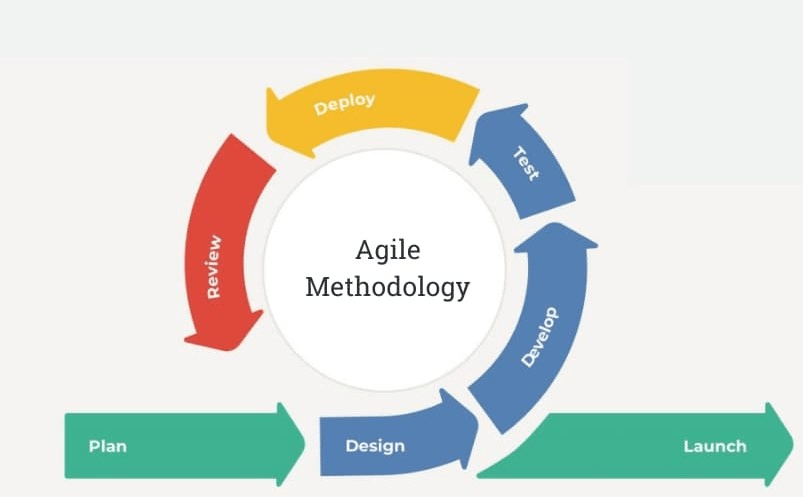
\includegraphics[width=0.85\linewidth,height=0.8\textheight,keepaspectratio]{Figures/agile_methodology.png}
\caption{Agile Methodology}
\label{fig:agilemethodology}
\end{figure}

\subsection{Justification of Proposing the Process Model}

The modules carry different levels of risk. Login, roles and exam set-up are well understood. Blocking Windows shortcut keys, the live dashboard, webcam analysis and running code in a Docker container were new to us. Waterfall would have forced us to fix all of these designs before we had built a prototype of any of them. With sprints we could try the risky parts early, integrate them step by step and adjust the plan. The sprint reviews at Weeks 16 and 32 also served as the FYP-I review and the final submission.

\subsection{Steps of Process Model}

The project runs over eight four-week sprints. Each sprint delivers modules that can be demonstrated. Table~\ref{tab:timeframe} in Chapter~\ref{chap:srs} gives the baseline schedule, and the text below it gives the progress at the FYP-I review. Every sprint goes through the following steps:
\begin{enumerate}[noitemsep]
\item \textbf{Product backlog:} FR1--FR12, grouped by module M1--M12 (Chapter~\ref{chap:srs}).
\item \textbf{Sprint planning:} a sprint goal and a sprint backlog in which each task has one WBS code and one owner.
\item \textbf{Development:} the module and its automated tests are written in the same sprint.
\item \textbf{Increment:} a task is done when its code and tests pass and its thesis section is updated.
\item \textbf{Sprint review:} the increment is demonstrated to the supervisor, who comments on it and on the backlog priorities.
\item \textbf{Schedule check:} if under 80\% of the story points are done, backlog items are moved or cut (Chapter~\ref{chap:spp}).
\item \textbf{Feedback:} review comments and accepted changes return to the product backlog.
\end{enumerate}
The baseline plan gives each sprint the following work:

\begin{itemize}[noitemsep]
\item \textbf{Sprint 1 (Weeks 1--4):} requirements, use cases, product backlog, architecture and scope approval.
\item \textbf{Sprint 2 (Weeks 5--8):} M1 and M7, with hardware-ID capture, device-bound student login, staff login and role-based access.
\item \textbf{Sprint 3 (Weeks 9--12):} M8 and M9, covering the exam wizard, question types, test cases, allowed applications and eligibility.
\item \textbf{Sprint 4 (Weeks 13--16):} M2, M3 and M4, covering the readiness check, practice exams, the student dashboard and the lockdown client.
\item \textbf{Sprint 5 (Weeks 17--20):} M5 and M10, with heartbeats, monitoring events and screenshots, and the live dashboard.
\item \textbf{Sprint 6 (Weeks 21--24):} M6 and M11, covering autosave, encrypted backup, test-case grading, TF-IDF theory scoring and the plagiarism matrix.
\item \textbf{Sprint 7 (Weeks 25--28):} M12, covering the hash-chained audit log, analytics, PDF reports, and Excel and evidence-ZIP exports.
\item \textbf{Sprint 8 (Weeks 29--32):} integration and system testing of all twelve modules, bug fixes, the final report and the demonstration.
\end{itemize}

\chapter{SOFTWARE REQUIREMENTS SPECIFICATION}
\label{chap:srs}

This chapter gives the Software Requirements Specification (SRS) for SmartExam \cite{srs1}. It states what the system must do, the quality levels it must meet, and the limits it works within. How each feature is built is covered in the design chapters.

\section{Introduction}
SmartExam has five user roles, several exam phases and strict fairness rules. We wrote this SRS after interviews with lab staff, prototype walk-throughs, two team brainstorming sessions and a review of existing tools (Section~\ref{sec:gathering}).

\subsection{Document Scope}
The SRS covers the twelve modules M1--M12: authentication and device binding, pre-exam verification and practice exams, the student exam dashboard, the secure exam environment, the live monitoring client service, submission and backup, user and role management, exam creation and configuration, eligibility and access control, the live proctoring dashboard, AI-assisted evaluation, and logs, analytics and the audit trail. It also sets ten non-functional requirements (NFR1--NFR10) for security, reliability, usability, performance, maintainability, data integrity, compatibility, connectivity, privacy, and backup and recovery.

Database schemas, API routes, screen layouts and deployment settings are not part of this chapter. They are given in the design chapters.

\subsection{Audience}
This document is written for everyone who builds, checks, runs or uses SmartExam. Each group reads it for a different reason:
\begin{itemize}
    \item \textbf{Software developers:} they use the requirements to know exactly what each module M1--M12 must do, so the desktop client, the API and the web panel are built to the same rules.
    \item \textbf{Testers:} they use each requirement and its limits as a test target, so every test case in Chapter~\ref{chap:testing} can be traced back to an FR or NFR.
    \item \textbf{Managers:} the supervisor and the project team use the requirements and the time frame to plan the sprints and to check progress at each review.
    \item \textbf{End-users:} students, teachers, invigilators and administrators can see what the system will do for them, from logging in and sitting an exam to watching a lab and grading answers.
    \item \textbf{Business and academic stakeholders:} the department and the evaluators can judge whether the scope is clear, fair to students and realistic for a two-semester FYP.
    \item \textbf{Data and quality assurance analysts:} they can see which logs, reports and exports the system produces and how the hash-chained audit log keeps that data trustworthy.
\end{itemize}

\section{Functional Requirements}
Functional requirements state what the system must do. Table~\ref{tab:functionalrequirements} lists them; FR$n$ belongs to module M$n$, and M11 has three (FR11.1--FR11.3).

\begin{table}[H]
\centering
\caption{Functional Requirements of SmartExam}
\label{tab:functionalrequirements}
\renewcommand{\arraystretch}{1.2}
\begin{tabularx}{\linewidth}{l>{\raggedright\arraybackslash}X}
\hline\hline
\textbf{Requirement ID} & \textbf{Description} \\
\hline
FR1 & User can log in, and a student can log in only from the workstation the account is bound to. \\
FR2 & User can run a readiness check before an exam and take practice exams. \\
FR3 & User can see the assigned exam, its readiness and eligibility status, and the results on the student dashboard. \\
FR4 & The system shall lock the workstation during an exam in Report or Enforce mode. \\
FR5 & The system shall send heartbeats, monitoring events, screenshots and webcam issues from the client to the server. \\
FR6 & The system shall save, back up and submit every answer without loss and return a submission receipt. \\
FR7 & User can manage accounts, roles, departments and courses. \\
FR8 & User can create, configure and announce exams with MCQ, coding and theory questions. \\
FR9 & User can set exam eligibility from attendance and assign invigilators and a workstation to each student. \\
FR10 & User can watch every student live and send warnings, extra time, unlocks or a forced submission. \\
FR11.1 & The system shall compile C and C++ answers and grade them against test cases. \\
FR11.2 & The system shall mark MCQ answers and suggest a score for theory answers. \\
FR11.3 & User can view the answer similarity between submissions and the pairs flagged above the threshold. \\
FR12 & User can verify the audit log and export analytics, PDF reports, an Excel workbook and an evidence ZIP. \\
\hline\hline
\end{tabularx}
\end{table}

\section{Non-Functional Requirements}
Non-functional requirements set the quality levels and operating limits of the system. They do not say what the system does but how well it must do it. For an exam system the most important ones are security and data integrity, because a fair exam depends on them. We give them the identifiers NFR1--NFR10 and split them into software quality attributes, based on ISO/IEC 25010:2023 \cite{iso25010}, and other non-functional requirements.

\subsection{Software Quality Attributes}
\label{sec:qualityattributes}
NFR1--NFR6 are the quality attributes of SmartExam. Where our name differs from the standard, the ISO/IEC 25010 characteristic is shown in brackets.
\begin{itemize}
    \item \textbf{Security (NFR1):} Passwords are stored as salted PBKDF2 hashes with 600,000 iterations \cite{owasp_pwd}, and older hashes are upgraded at the next login \cite{nist80063b}. Access tokens expire after 30 minutes, refresh tokens can be used only once, and each IP address may try to log in at most 10 times a minute. Every request except login, token refresh and the health check needs a valid JWT \cite{rfc7519} and a permitted role.
    \item \textbf{Reliability (NFR2):} A network outage of any length shall not lose an answer. Every edit reaches the encrypted local backup within about 1 s, failed saves and events are queued and sent in order later, and a restarted client resumes the session.
    \item \textbf{Usability (NFR3, interaction capability):} A student shall be able to log in, pass the readiness check and start an exam using only the on-screen instructions. Every refusal shows its reason, and final actions ask for confirmation.
    \item \textbf{Performance (NFR4, performance efficiency):} With 40 desktop clients sending heartbeats every 10 s, login, exam start, answer saves and heartbeats shall complete within 2 s at the 95th percentile.
    \item \textbf{Maintainability (NFR5):} The system is one ASP.NET Core 9 API organised by module. Every module M1--M12 has automated tests (xUnit and Playwright) that run headless, so a full regression needs no lab PC.
    \item \textbf{Data Integrity (NFR6, security: integrity):} The server enforces the deadline, so a changed client clock cannot extend an exam. A save older than the stored answer is refused, each submission returns a SHA-256 receipt, and the hash-chained audit log shows any changed row or gap.
\end{itemize}

\subsection{Other Non-Functional Requirements}
\label{sec:othernfr}
NFR7--NFR10 fix where and how the system runs and what happens to its data:

\textbf{Compatibility (NFR7):} The client runs on Windows 10 (22H2) or Windows 11 with the .NET 9 Desktop Runtime and was tested on Windows 11. The web panel runs in Chrome or Edge 111 or later.

\textbf{Connectivity (NFR8):} The client and the web panel call the API over REST, with HTTPS behind a TLS endpoint in a lab deployment; no local lab server is needed. The web dashboard gets live updates, and the desktop client receives staff commands with its next heartbeat (every 10 s).

\textbf{Privacy (NFR9):} No face recognition or identity matching is performed. Webcam frames are analysed on the PC, and webcam snapshots and screenshots can be viewed only by the exam's owner, its invigilators and administrators, and are deleted after 30 days.

\textbf{Backup and Recovery (NFR10):} The Neon PostgreSQL database can be restored to a point in time within the provider's restore window, and a crash on a student PC loses at most the last second of typing. Screenshots and webcam snapshots are kept on the API server's disk, which the database backup does not cover, so the evidence folder shall be copied to backed-up storage after each exam.

\section{Requirement Gathering Techniques Used}
\label{sec:gathering}
To understand what the users of SmartExam need, we used structured interviews, paper prototypes, two brainstorming sessions and an analysis of existing systems \cite{elicit1, sommerville}.

\subsection{Interviews}
We asked teachers and lab coordinators how practical exams run today. Two needs came up most: watching workstations live, and keeping evidence that can settle disputes later.

\subsection{Prototyping}
We showed users paper prototypes of the login, dashboard, exam and submission screens \cite{sommerville}. Their feedback added a countdown timer on the exam screen, a live alert count at the top of each student's tile on the live dashboard, and one question per screen.

\subsection{Brainstorming Session 1: Academic Workflow}
We mapped the life cycle of a lab exam and the manual steps that cost staff the most time. This set the order in which we built the foundation: role management, exam configuration and seat assignment (Sprints 2 and 3).

\subsection{Brainstorming Session 2: Monitoring and Reporting}
We discussed monitoring, proctoring and reports. Face recognition was left out of scope because of privacy concerns and the effort of reliable identity matching on lab webcams, so the webcam checks look only at the camera state and the faces in view; the coarse head-pose and phone checks were added later. We also agreed that every exam needs reports on attendance, violations and scores; these became separate PDF exports beside an exam summary PDF.

\subsection{Analysis of Existing Systems}
Section~\ref{sec:existingsystems} reviews ten existing tools, and Table~\ref{tab:comparison} compares them feature by feature. No tool binds a student to a lab workstation or runs code against test cases, and only MOSS checks code for plagiarism. Some tools offer lockdown or live monitoring, but none combines them with these features for an exam in a physical lab. These gaps set FR1, FR4, FR9, FR10, FR11.1 and FR11.3.

\section{Time Frame}
The project runs over eight four-week sprints (Weeks 1--32), each ending with a working increment for supervisor review. Table~\ref{tab:timeframe} gives the main work and the duration of each sprint.

\begin{table}[H]
\centering
\caption{Time Frame}
\label{tab:timeframe}
\renewcommand{\arraystretch}{1.2}
\begin{tabularx}{\linewidth}{>{\raggedright\arraybackslash}Xr}
\hline\hline
\textbf{Phase} & \textbf{Duration} \\
\hline
Sprint 1: Requirement analysis, product backlog, architecture and scope approval & 4 weeks \\
Sprint 2 (M1, M7): Login, hardware-ID device binding, JWT and roles & 4 weeks \\
Sprint 3 (M8, M9): Exam creation, test cases, allowed apps, eligibility and seats & 4 weeks \\
Sprint 4 (M2, M3, M4): Readiness check, practice exams, student dashboard and lockdown & 4 weeks \\
Sprint 5 (M5, M10): Monitoring client and live proctoring dashboard & 4 weeks \\
Sprint 6 (M6, M11): Autosave and backup, test-case grading, theory scoring and plagiarism & 4 weeks \\
Sprint 7 (M12): Hash-chained audit log, analytics, PDF reports, and Excel and evidence-ZIP exports & 4 weeks \\
Sprint 8: Integration, end-to-end testing, bug fixing, documentation and demo & 4 weeks \\
\hline
\textbf{Total Duration} & \textbf{32 weeks} \\
\hline\hline
\end{tabularx}
\end{table}

Table~\ref{tab:timeframe} is the baseline plan. It fits the FYP-I proposal's timeline (February 2026 to March 2027) into two semesters: Week 1 began in March 2026 and Week 32 ended with the final test run on 26 October 2026, and installation in the labs follows submission. At the FYP-I review (Week 16), M1, M3, M7, M8, M9 and M10 (at heartbeat level) were working; M2, M4 and refresh-token rotation moved into Sprints 5--8 with the remaining modules.

\chapter{SOFTWARE PROJECT PLAN}
\label{chap:spp}

This chapter gives the plan we followed to build SmartExam in 32 weeks \cite{pmbok6}: the deliverables, the schedule, how the team was managed, and the project risks with our response to each.

\textbf{Project Overview.} SmartExam runs a programming lab exam from start to finish: device-bound sign-in, lockdown on the lab PCs, live supervision, AI-assisted marking and an audit trail (Chapter~\ref{chap:introduction}).

\textbf{Project Organization.} Three members share the work, and each owns one area (Section~\ref{sec:managerial}). Our supervisor reviews the result of every sprint.

\textbf{Project Schedule.} The work runs in eight four-week sprints (Table~\ref{tab:timeframe}). The milestones are in Section~\ref{sec:milestones}, and the Gantt chart and critical path in Section~\ref{sec:scheduling}.

\textbf{Resource Allocation.} The people, hardware, software and services we use are listed in Table~\ref{tab:resources}.

\section{Deliverables of the Project}

A deliverable is an output of the project that is handed over and can be checked \cite{del1}. Our deliverables are:
\begin{itemize}
    \item \textbf{Software Requirements Specification:} the functional and non-functional requirements of Chapter~\ref{chap:srs} \cite{srs1}.
    \item \textbf{Design documents:} the use case model, the system design diagrams, the user interface designs and the database design (Chapters~4 to~6).
    \item \textbf{Working system:} the student desktop client for the lab PCs, the web panel for staff and the server with its database, covering all twelve modules.
    \item \textbf{Test plan and test report:} the test cases and their results (Chapter~\ref{chap:testing}).
    \item \textbf{Final report and presentation:} this report and the slides for the final demonstration.
\end{itemize}

\section{Software Project Management Plan}

\subsection{Project Planning}

We planned the work in eight four-week sprints (Table~\ref{tab:timeframe}). Sprint~1 covers requirements and design, Sprints~2--7 build the modules, and Sprint~8 is kept for integration, testing and the demonstration. A task is done when its code and tests pass and its part of this report is updated. The work is broken down in the Work Breakdown Structure (WBS) of Section~\ref{sec:wbs} \cite{wbs1}.

\subsubsection{Milestones Plan}
\label{sec:milestones}

Table~\ref{tab:milestones} lists the seven milestones of the plan. Each row gives the week in which the milestone falls due and the evidence that shows it was reached.

\begin{table}[!ht]
\centering
\caption{Project Milestones}
\label{tab:milestones}
{\small\renewcommand{\arraystretch}{1.1}
\begin{tabularx}{\textwidth}{c>{\raggedright\arraybackslash}X>{\centering\arraybackslash}p{1.4cm}>{\raggedright\arraybackslash}p{4.9cm}}
\hline\hline
\textbf{ID} & \textbf{Milestone} & \textbf{Week} & \textbf{Evidence of completion} \\
\hline
MS1 & FYP-I proposal submitted & Before 1 & Proposal, 24 Feb 2026 \\
MS2 & Requirements, product backlog and architecture agreed & 4 & Scope approved \\
MS3 & Login, device binding and roles working (M1, M7) & 8 & Module tests pass \\
MS4 & FYP-I review & 16 & FYP-I report submitted, 18 Jun 2026 \\
MS5 & Supervision, submission and evaluation working (M5, M6, M10, M11) & 24 & Module tests pass \\
MS6 & All twelve modules merged (M12 last) & 28 & Module tests pass (M2 and M4 tests finished in Sprint~8) \\
MS7 & Final test run and submission & 32 & Full test run, 26 Oct 2026 \\
\hline\hline
\end{tabularx}}
\end{table}

\subsubsection{Documentation Plan}

The report is kept in step with the code:
\begin{itemize}[nosep]
    \item The report is written in LaTeX, and the section a task changes is updated in that task.
    \item Diagrams are kept as text sources beside the report, so they are redrawn when the design changes.
    \item Each version of the report is recorded in the Revision History, and supervisor feedback goes into the next sprint's backlog.
\end{itemize}

\subsubsection{Resources Plan}
\label{sec:resources_plan}

Table~\ref{tab:resources} lists the resources the project uses, one row for each kind. The project has no budget, so every service is a free plan or is off by default.

\begin{table}[!ht]
\centering
\caption{Project Resources}
\label{tab:resources}
{\small\renewcommand{\arraystretch}{1.2}
\begin{tabularx}{\textwidth}{>{\raggedright\arraybackslash}p{2.2cm}>{\raggedright\arraybackslash}X}
\hline\hline
\textbf{Resource} & \textbf{Allocation} \\
\hline
People & Three members, each owning one area (Section~\ref{sec:managerial}); the supervisor reviews every sprint. \\
Hardware & Our own PCs for development and the automated tests; Windows lab PCs, with webcams where an exam needs one, for the manual lockdown and webcam checks. \\
Software & .NET~9 (server and desktop client), React (web panel), PostgreSQL, OpenCV with the YuNet and YOLOX-Nano models, Docker with a GCC compiler image, xUnit, Playwright, Git, and LaTeX with PlantUML for this report. \\
Services & Neon cloud PostgreSQL (free plan), an e-mail account for notifications, and an optional AI language-model service for theory marking that is off by default. \\
Budget & None: no paid service is used. \\
\hline\hline
\end{tabularx}}
\end{table}

\subsubsection{Quality Plan}

Quality is checked inside every sprint, not only at the end:
\begin{itemize}[nosep]
    \item Each module is tested in its own sprint with server, web and desktop tests, and the full test suite is rerun after each group of fixes.
    \item Checks that need a real lab PC are kept on a manual lab checklist (Chapter~\ref{chap:testing}).
    \item AI output is only a suggestion: the teacher reviews and can change every mark, and no violation leads to an automatic penalty.
    \item The supervisor reviews each increment at the end of the sprint.
\end{itemize}

\subsection{Project Scheduling}
\label{sec:scheduling}

\subsubsection{Gantt Chart}

Table~\ref{tab:cpm} lists the nine project activities with their modules, their length in weeks and the activities each must wait for. The Gantt chart and the critical path network are both drawn from this table.

\begin{table}[!htbp]
\centering
\caption{Project Activities, Durations and Dependencies}
\label{tab:cpm}
\renewcommand{\arraystretch}{1.2}
\begin{tabular}{c>{\raggedright\arraybackslash}p{7.2cm}lcc}
\hline\hline
\textbf{ID} & \textbf{Activity} & \textbf{Modules} & \textbf{Weeks} & \textbf{Depends on} \\
\hline
A & Requirements, backlog and architecture & -- & 4 & -- \\
B & Authentication and device binding & M1 & 4 & A \\
C & User and role management & M7 & 2 & A \\
D & Exam creation and eligibility & M8, M9 & 4 & B, C \\
E & Readiness check, student dashboard and lockdown & M2--M4 & 4 & D \\
F & Monitoring client and live proctoring dashboard & M5, M10 & 4 & E \\
G & Submission, backup and AI-assisted evaluation & M6, M11 & 4 & F \\
H & Audit log, analytics and reports & M12 & 4 & G \\
I & Integration, system testing, documentation and demo & All & 4 & H \\
\hline\hline
\end{tabular}
\end{table}

Figure~\ref{fig:ganttchart} places the activities of Table~\ref{tab:cpm} on Weeks 1--32 \cite{gantt1}. Red bars lie on the critical path, and the diamonds mark the FYP-I review and the final submission.

\begin{figure}[!htbp]
\centering
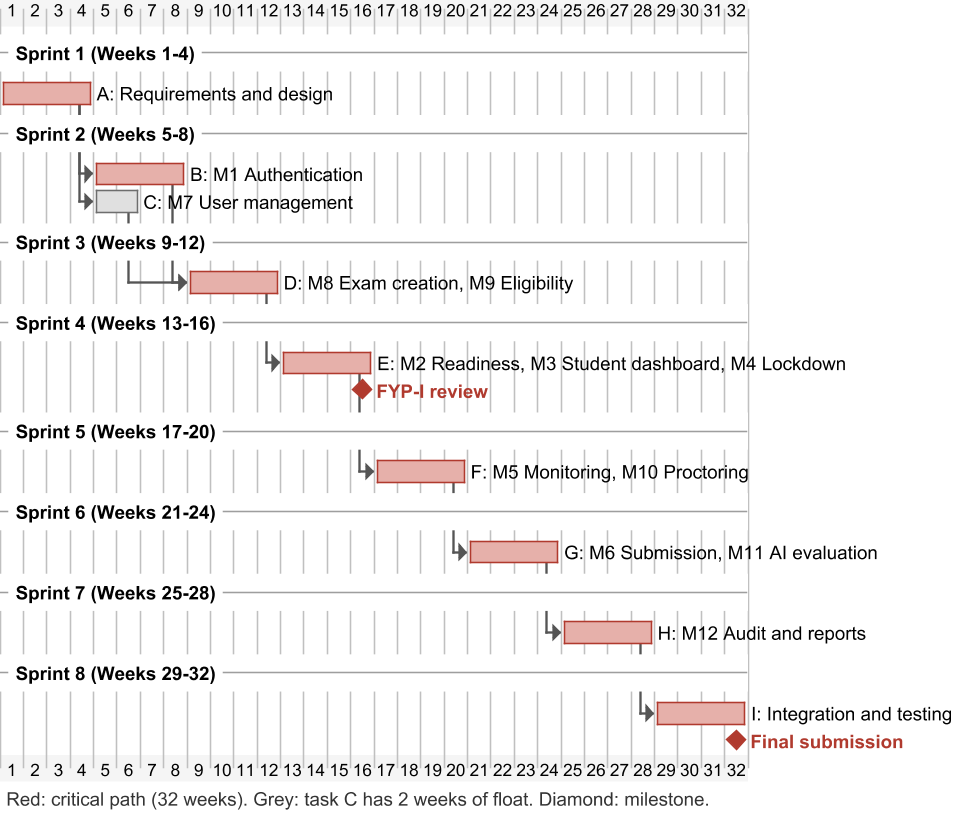
\includegraphics[width=\linewidth,height=0.8\textheight,keepaspectratio]{Figures/gantt_chart.png}
\caption{Project Gantt Chart (Baseline Plan, Eight Sprints)}
\label{fig:ganttchart}
\end{figure}

\DiagramBarrier
\subsubsection{Work Breakdown Structure}
\label{sec:wbs}

Figure~\ref{fig:wbs} splits the project into four main work packages \cite{wbs1}. Under Module Development, each module is one work package that includes its own tests.

\begin{figure}[!htbp]
\centering
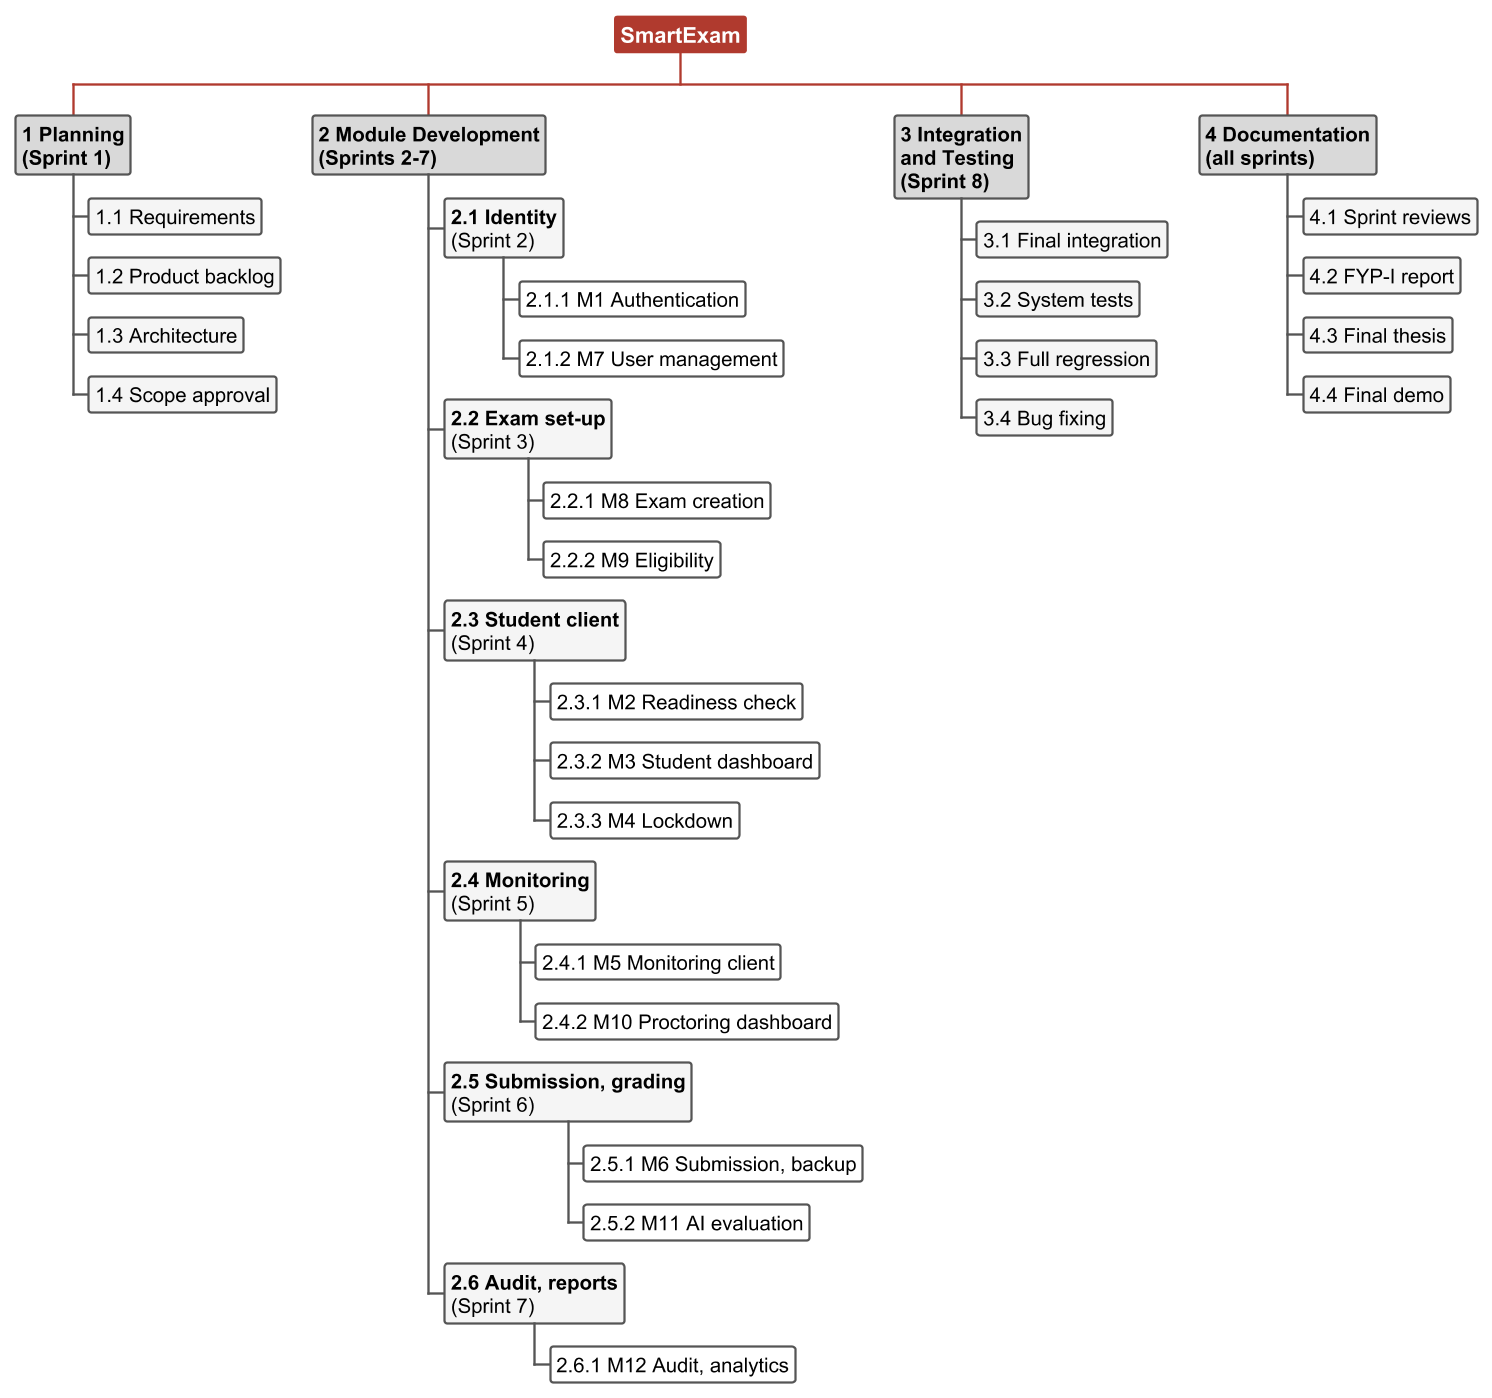
\includegraphics[width=\linewidth,height=0.8\textheight,keepaspectratio]{Figures/work_breakdown_structure.png}
\caption{Work Breakdown Structure}
\label{fig:wbs}
\end{figure}

\DiagramBarrier
\subsubsection{Critical Path Method}

The critical path is the longest chain of dependent activities; a delay on it delays the whole project \cite[Sec.~6.5.2.2]{pmbok6}. Since almost all our work lies on it, we tracked each sprint with a burn-down chart \cite{scrum1}; when less than 80\% of a sprint's story points were done at the review, backlog items were moved or cut.

Figure~\ref{fig:criticalpath} shows the network of Table~\ref{tab:cpm}. The path A--B--D--E--F--G--H--I takes 32 weeks; only C, which runs beside B, has two weeks of float.

\begin{figure}[!htbp]
\centering
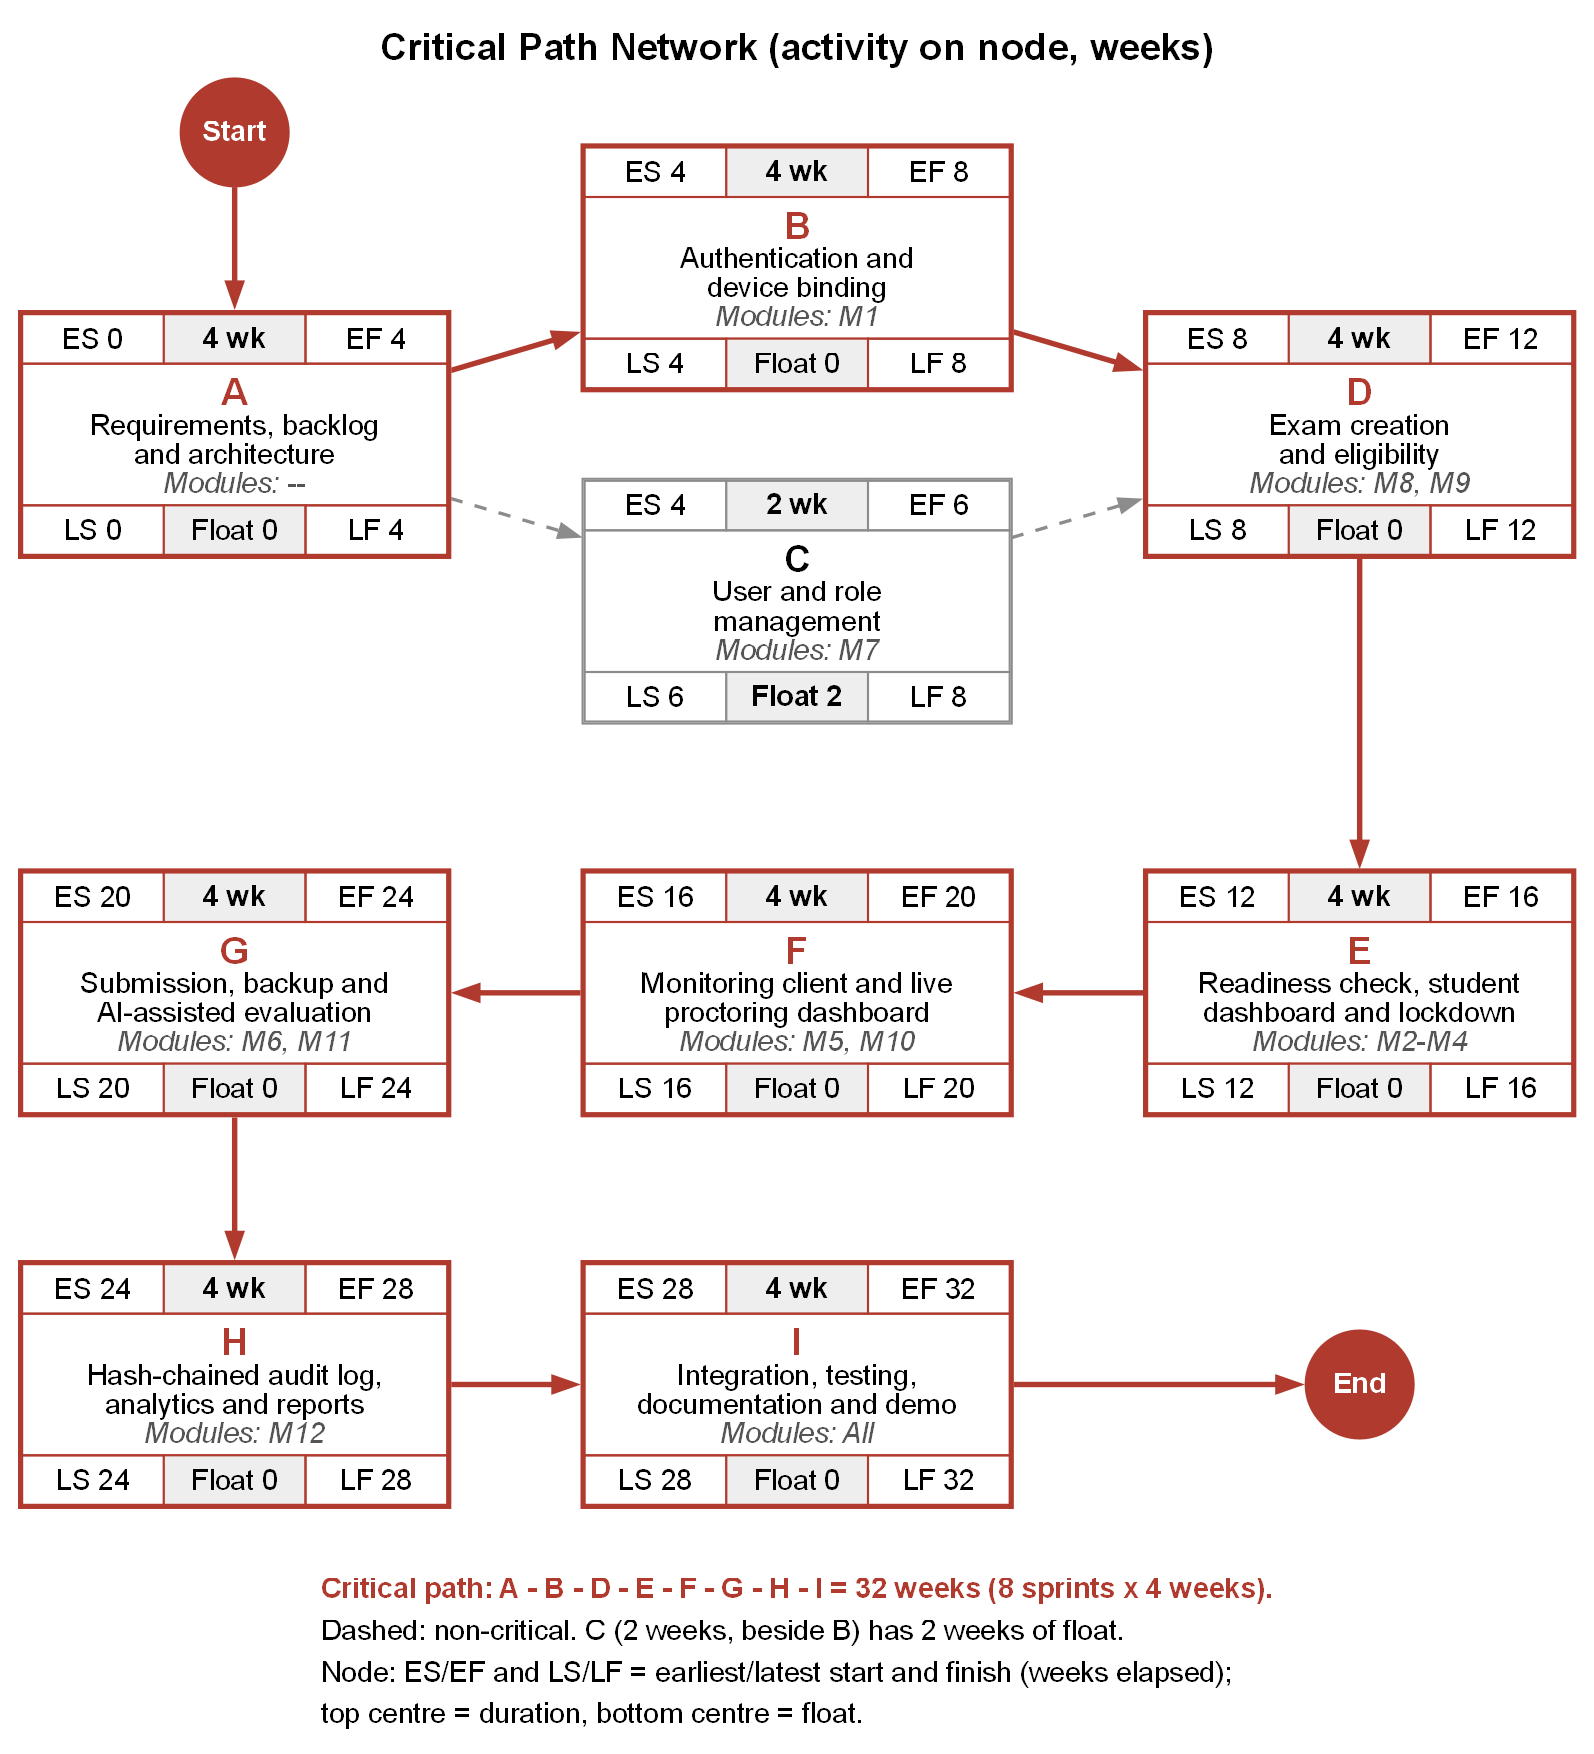
\includegraphics[width=\linewidth,height=0.8\textheight,keepaspectratio]{Figures/critical_path.png}
\caption{Critical Path Network}
\label{fig:criticalpath}
\end{figure}
\DiagramBarrier

\section{Managerial Process}
\label{sec:managerial}

Our team has three members, and each owns one area: Muhammad Haider Ali is the project manager and owns the architecture, the server and the database; Zain Ali Mehmood owns the student desktop client, lockdown and monitoring; and Roshaan Ali Shah owns AI evaluation, plagiarism detection and testing. We follow Scrum in a light form \cite{scrumguide2020}: each sprint starts with planning and ends with a review with our supervisor, short written check-ins replace the daily stand-up, and a blocker unsolved after 24 hours goes to a team discussion.

\textbf{Changes since the FYP-I proposal.} The twelve proposal modules were regrouped: role management became M7, eligibility became its own module (M9), and behaviour analysis became the violation classifier used in live monitoring. We added the Invigilator and SuperAdmin roles, chose PostgreSQL on Neon as the database, and run the grading inside the server instead of in a separate Python service.

\subsection{Management Objectives and Priorities}
\label{sec:priorities}

Our objective is a system that lets a teacher run a fair lab exam from start to finish. We measure progress with four goals:
\begin{itemize}[nosep]
    \item Deliver all twelve modules, each with its own tests, within the 32 weeks.
    \item Test every functional requirement FR1--FR12 (Chapter~\ref{chap:testing}).
    \item Use no paid services.
    \item Show the supervisor a working increment at the end of every sprint.
\end{itemize}

When time is short, we protect work in this order, and lower items are cut first:
\begin{enumerate}[nosep]
    \item \textbf{Foundations:} accounts and roles, exam creation and the student dashboard (M7, M8, M3).
    \item \textbf{Exam integrity:} device binding, the readiness check, eligibility and seats, and lockdown (M1, M2, M9, M4).
    \item \textbf{No lost work:} autosave, encrypted backup and the server deadline (M6).
    \item \textbf{Live supervision:} monitoring client and proctoring dashboard (M5, M10).
    \item \textbf{Evaluation support:} test-case marking, theory scoring and plagiarism checks (M11).
    \item \textbf{Reporting:} audit log, analytics and reports (M12).
\end{enumerate}

\subsection{Assumptions and Constraints}
\label{sec:constraints}

\textbf{Assumptions}
\begin{itemize}[nosep]
    \item Lab PCs run Windows 10 or 11 (we tested on Windows 11), and we can install the client with administrator rights.
    \item Each PC reaches the server over the lab network; short outages may happen.
    \item Each student uses one assigned PC, with a webcam when the exam needs one.
    \item Teachers supply the test cases and model answers used for automatic marking.
\end{itemize}

\textbf{Constraints}
\begin{itemize}[nosep]
    \item Three members and 32 weeks over two semesters.
    \item No budget: we use the Neon free plan, and the AI features run offline on the CPU (text-similarity scoring, YuNet face detection \cite{yunet} and YOLOX-Nano phone detection \cite{yolox}). Marking with an online language model is off by default.
    \item The client runs only on Windows and cannot block Ctrl+Alt+Del.
    \item Isolated running of C and C++ answers needs Docker on the server. Without it, a local compiler that is not isolated is used, and with no compiler the answer is left for the teacher.
    \item For privacy, no face recognition is done. Screenshots and webcam pictures can be viewed only by the exam's owner, the staff assigned to supervise it and administrators, and are deleted after 30 days.
\end{itemize}

\section{Project Risk Management}

We identify the risks to the project early, rate them, and plan a response for each \cite{risk1}.

\subsection{Risk Management Plan}

\subsubsection{Purpose}

The plan sets how we find, rate, answer and track the risks that could stop a fair exam, lose student work or delay the 32-week schedule, and who does each step.

\subsubsection{Roles and Responsibilities}

\begin{description}[nosep]
    \item[Risk manager:] Muhammad Haider Ali, the project manager, keeps the risk register (Table~\ref{tab:risk_ident}).
    \item[Risk owners:] each member rates the risks of their own area and carries out the response. The Owner column uses PM for Muhammad Haider Ali (server, database and schedule), Client for Zain Ali Mehmood (desktop client) and AI/QA for Roshaan Ali Shah (AI evaluation and testing).
    \item[Team members:] all three members report a new risk at the written check-ins.
    \item[Stakeholder:] our supervisor, Ms.~Zainab Iftikhar Chaudhary, sees the risk register at each sprint review.
\end{description}

\subsection{Risk Management Activities}

\subsubsection{Risk Identification}

Table~\ref{tab:risk_ident} lists the twelve risks we found in SmartExam, each with its cause. For each risk it gives the category, the chance that it happens, what it would harm, its score and its owner.

{\footnotesize\setlength{\tabcolsep}{3pt}\renewcommand{\arraystretch}{1.15}
\begin{longtable}{@{}c>{\raggedright\arraybackslash}p{4.25cm}>{\raggedright\arraybackslash}p{1.65cm}>{\raggedright\arraybackslash}p{2.0cm}>{\raggedright\arraybackslash}p{3.55cm}>{\centering\arraybackslash}p{1.3cm}>{\raggedright\arraybackslash}p{1.2cm}@{}}
\caption{Risk Identification}\label{tab:risk_ident}\\
\hline\hline
\textbf{ID} & \textbf{Risk and its cause} & \textbf{Category} & \textbf{Probability} & \textbf{Impact (what it harms)} & \textbf{Score} & \textbf{Owner} \\
\hline
\endfirsthead
\multicolumn{7}{c}{\tablename~\thetable{} -- continued from previous page}\\
\hline\hline
\textbf{ID} & \textbf{Risk and its cause} & \textbf{Category} & \textbf{Probability} & \textbf{Impact (what it harms)} & \textbf{Score} & \textbf{Owner} \\
\hline
\endhead
\hline\hline
\endlastfoot
R1 & Antivirus or a Windows update blocks the keyboard lock or the Task Manager block, so the lockdown cannot stop Alt+Tab or the Windows key. & Technical & Medium (30\%) & High: a student can leave the exam window unseen. & 6 High & Client \\
R2 & Some lab PCs have no webcam, or a broken one, so webcam monitoring cannot run for those seats. & Resource & High (60\%) & Medium: no webcam evidence for those students; the rest of the monitoring still works. & 6 High & Client \\
R3 & The lab network is unstable (loose cables, switch faults), so a PC loses the server during an exam. & Technical & Medium (40\%) & High: answers, monitoring data and exam time of the student. & 6 High & Client \\
R4 & The Neon cloud database has an outage, or the project reaches a limit of the free plan. & External & Low (15\%) & High: sign-in, saving and the live dashboard stop for every student. & 3 Medium & PM \\
R5 & Docker is not available on the PC that runs the server, so student code cannot run in an isolated container. & Technical & Medium (40\%) & Medium: student code runs without isolation, or coding answers wait for manual marking. & 4 Medium & AI/QA \\
R6 & Short answers or code given by the teacher make honest answers look alike, so the plagiarism check flags them falsely. & Technical & Medium (35\%) & Medium: honest students are suspected, and the teacher spends time reviewing pairs. & 4 Medium & AI/QA \\
R7 & A lab PC gets a new disk or motherboard after a repair, so its hardware ID changes and the student bound to it is refused at sign-in. & Technical & Medium (25\%) & Medium: the student cannot start the exam on time. & 4 Medium & PM \\
R8 & The e-mail account's password expires or the mail server refuses the message, so notice e-mails are not delivered. & External & Medium (30\%) & Low: students learn about a scheduled exam or released grades late; no data is lost. & 2 Low & PM \\
R9 & A lab PC's clock is wrong, so its exam timer or start time differs from the server's. & Technical & Low (15\%) & Medium: a student starts early or late, or loses exam time. & 2 Low & Client \\
R10 & A member is ill or busy with other courses during a critical sprint. & Resource & Medium (30\%) & Medium: the work of one area stops for one or two weeks. & 4 Medium & PM \\
R11 & New features asked for during reviews grow the backlog beyond the 32 weeks (scope creep). & Schedule & High (70\%) & Medium: later modules and their tests are squeezed into the last sprint. & 6 High & PM \\
R12 & Screenshots and webcam pictures show students' screens and faces; a leak or misuse would breach their privacy. & Security & Low (10\%) & High: student privacy and trust in the department. & 3 Medium & PM \\
\end{longtable}}

\subsubsection{Risk Analysis}

Each risk is rated on a probability and impact matrix \cite{iec31010} (Table~\ref{tab:risk_matrix}). Probability is Low up to 20\%, Medium 21--50\% and High above 50\%; with Low~=~1, Medium~=~2, High~=~3, the score is probability $\times$ impact: 6--9 High, 3--4 Medium, 1--2 Low.

\begin{table}[!ht]
\centering
\caption{Risk Likelihood and Impact Assessment}
\label{tab:risk_matrix}
{\small\renewcommand{\arraystretch}{1.3}
\begin{tabular}{@{}l>{\centering\arraybackslash}p{3.3cm}>{\centering\arraybackslash}p{3.3cm}>{\centering\arraybackslash}p{3.3cm}@{}}
\hline\hline
\textbf{Probability} & \textbf{Low impact} & \textbf{Medium impact} & \textbf{High impact} \\
\hline
High (above 50\%) & 3 (none) & 6: R2, R11 & 9 (none) \\
Medium (21--50\%) & 2: R8 & 4: R5, R6, R7, R10 & 6: R1, R3 \\
Low (up to 20\%) & 1 (none) & 2: R9 & 3: R4, R12 \\
\hline\hline
\end{tabular}}
\par\vspace{3pt}
{\footnotesize\begin{minipage}{\linewidth}
Impact: Low = only a delay or an inconvenience; Medium = affects one student, one exam or one sprint; High = harms the fairness of an exam, loses student work or threatens the deadline.
\end{minipage}}
\end{table}

\subsubsection{Risk Response Planning}

We mitigate all twelve risks. Table~\ref{tab:risk_response} gives each risk's early warning sign, what we did to lower it, what we do if it still happens, and its status at the final submission.

{\footnotesize\setlength{\tabcolsep}{3pt}\renewcommand{\arraystretch}{1.15}
\begin{longtable}{@{}c>{\raggedright\arraybackslash}p{2.9cm}>{\raggedright\arraybackslash}p{5.2cm}>{\raggedright\arraybackslash}p{3.9cm}>{\raggedright\arraybackslash}p{1.8cm}@{}}
\caption{Risk Mitigation and Contingency Plan}\label{tab:risk_response}\\
\hline\hline
\textbf{ID} & \textbf{Trigger (early warning)} & \textbf{Mitigation taken} & \textbf{Contingency if it happens} & \textbf{Status} \\
\hline
\endfirsthead
\multicolumn{5}{c}{\tablename~\thetable{} -- continued from previous page}\\
\hline\hline
\textbf{ID} & \textbf{Trigger (early warning)} & \textbf{Mitigation taken} & \textbf{Contingency if it happens} & \textbf{Status} \\
\hline
\endhead
\hline\hline
\endlastfoot
R1 & Secure mode fails in the readiness check, or a ``Lockdown degraded'' alert appears on the student's tile. & The readiness check tests that the keyboard lock can be installed before the exam. If the lock or the Task Manager block fails during the exam, the invigilator is alerted at once, and screenshots and focus-loss events are still recorded. & The lab adds the client to the antivirus allow-list; until then the invigilator watches that seat in person. & Built; lab test pending \\
R2 & The camera item fails in the readiness check, or a ``camera unavailable'' event appears on a tile. & The webcam is a per-exam setting. When it is on, the readiness check confirms a working, uncovered camera before the start. A camera that stops during the exam is reported once, and the exam goes on. & Seat the student at a PC with a camera, or turn off the webcam setting before the exam and watch those seats in person. & Built; lab test pending \\
R3 & A tile shows the student as disconnected after 30~s without a heartbeat. & Every edit is saved within about 1~s to an encrypted backup on the PC. Answers and monitoring events that fail to send are queued and sent again when the link returns, and answers are restored after a crash. & The student keeps working offline while the cable is checked; the invigilator can give that student extra minutes. & Built; lab test pending \\
R4 & Sign-in or save errors from the server, or database usage near the free-plan limit. & Heartbeats are stored only when they change or once a minute. Screenshots are kept as files on the server, not in the database, and are deleted after 30 days. We take a full database backup before each change to its structure. & Answers wait in the client's backup and queue. For a long outage, the server is moved to a local PostgreSQL database restored from the latest backup. & Open; has not occurred \\
R5 & Marking results show the ``not isolated'' label, or coding answers wait for manual marking. & The server checks for Docker before each marking run. Without it, a local compiler runs each answer with time and memory limits and the result is labelled ``not isolated''; with no compiler, the answer is left for the teacher. & Install Docker on the server, or the teacher marks the coding answers by hand; AI marks are only suggestions. & Built and tested \\
R6 & Many pairs are flagged in one exam, or the matching lines are mostly code the teacher gave. & Code is compared as tokens, so comments, spacing and variable names do not matter. Only pairs at or above the exam's threshold (70\% by default) are flagged, with the matching lines shown side by side. A flag never changes a mark. & The teacher reviews each flagged pair and decides; the threshold can be raised for the next exam. & Built and tested \\
R7 & Sign-in is refused because the account is bound to another device; the audit log records the mismatch. & An administrator can reset a student's device binding on the Device Bindings page. The reset is written to the audit log, the student's old sessions are signed out, and the next sign-in binds the new PC. & Reset the binding before the exam, or move the student to a spare PC, reassign the seat and reset the binding. & Built and tested \\
R8 & Failed e-mails in the server log, or students report that no e-mail arrived. & Every notice is first saved in SmartExam and shown in the student's notifications. A failed e-mail is logged and does not stop the action that sent it. & Renew the e-mail password; the teacher announces the exam in class. & Partly built: failed e-mails are logged, not resent \\
R9 & The system clock item fails in the readiness check. & The server's clock is the reference: the readiness check fails when the PC's clock is more than 60~s off, the exam timer counts down the time left sent by the server, and the server refuses answers after the deadline plus a 2-minute grace. & Set the PC's clock from the network time service; the invigilator can give extra minutes. & Built and tested \\
R10 & A task is blocked for more than 24 hours, or a member misses the check-ins. & Work is split by area in one shared Git repository, and every module has its own tests, so another member can take it over. & Move the member's tasks to the others and cut low-priority items in the order of Section~\ref{sec:priorities}. & Open; watched at each review \\
R11 & Less than 80\% of a sprint's story points are done at the review. & A change is accepted only if it fits in the current sprint and does not put a working module at risk; otherwise it goes to the future-work list. Sprint~8 adds no new modules. & Move or cut backlog items in the order of Section~\ref{sec:priorities}. & Occurred after FYP-I (M2, M4 moved to Sprints 5--8); closed in Week~32 \\
R12 & A student complaint, or captures seen by someone outside the exam's staff. & No face recognition is done. Only the exam's owner, its assigned supervisors and administrators can view captures, every user must sign in, and captures are deleted after 30 days. & Sign the account out, check the audit log and delete the affected captures. & Built and tested \\
\end{longtable}}

\subsubsection{Risk Monitoring and Control}

The owners re-rate their risks at every sprint review and update the status column of Table~\ref{tab:risk_response}. A risk that rises to High is taken to the supervisor with a recovery action. A new risk takes the next free ID, and a risk is closed when it can no longer occur; for example, R11 closed with the final test run in Week~32.

\chapter{FUNCTIONAL ANALYSIS AND MODELING}

\section{Use Case Modeling}

A use case model shows what a system does for its users, without going into how it is built \cite{uml_systems_analysis}. SmartExam has 12 use cases, one for each module M1 to M12. The same 12 use cases, with the same numbers and names, are used for the user stories and use case tables in this chapter, the activity and sequence diagrams in Chapter~5 and the unit test cases in Chapter~7.

\DiagramFig{width=\linewidth,height=0.8\textheight,keepaspectratio}{use_case_diagram.png}%
{Use Case Diagram of SmartExam}{fig:usecase_diagram}%
{Figure~\ref{fig:usecase_diagram} shows the five actors and the 12 use cases. Every user signs in (UC-01); the student then uses UC-02 to UC-06 and the staff use UC-07 to UC-12.}

\subsection{User Stories}

A user story states what a user wants and why \cite{user_stories_applied}. The stories below are grouped by actor, and each one names the use case it belongs to.

\subsubsection{Student}
\begin{itemize}[nosep]
    \item As a student, I want to log in on my lab PC and have my account bound to it, so that nobody can sit my exam from another machine (UC-01).
    \item As a student, I want to run a readiness check and a practice exam before the real exam, so that problems with my PC are found early (UC-02).
    \item As a student, I want to see my assigned exam, its countdown and my eligibility, and start it when it opens, so that I know whether and when I can sit it (UC-03).
    \item As a student, I want to see my results, violation history and notifications on the web portal after the exam, so that I can follow my progress (UC-03).
    \item As a student, I want to sit the exam in a locked fullscreen window, so that every candidate works under the same rules (UC-04).
    \item As a student, I want my PC to send its status and screenshots during the exam, so that the invigilator can see that I am online and working (UC-05).
    \item As a student, I want my answers saved automatically and a receipt when I submit, so that my work is not lost if the network or the PC fails (UC-06).
\end{itemize}

\subsubsection{Teacher}
\begin{itemize}[nosep]
    \item As a teacher, I want to sign in to the web panel with my email and password, so that only I can work on my exams (UC-01).
    \item As a teacher, I want to create an exam with MCQ, coding and theory questions and set its lockdown rules, so that the exam runs under the rules I chose (UC-08).
    \item As a teacher, I want to send an announcement about an exam, also by email if I choose, so that every student knows the schedule (UC-08).
    \item As a teacher, I want to import attendance, set eligibility, override single students and assign seats and invigilators, so that only eligible students sit the exam at their own PCs (UC-09).
    \item As a teacher, I want to watch every student live and warn, add time, unlock the PC or force a submission, so that I can deal with problems during the exam (UC-10).
    \item As a teacher, I want coding answers run against test cases and theory answers given suggested marks, so that marking is faster while I keep the final mark (UC-11).
    \item As a teacher, I want to see how similar the submissions are, so that I can check likely copying myself (UC-11).
    \item As a teacher, I want to download an exam's reports and evidence, so that I have a record of the exam (UC-12).
\end{itemize}

\subsubsection{Invigilator}
\begin{itemize}[nosep]
    \item As an invigilator, I want to sign in to the web panel, so that I can open the exams I am assigned to (UC-01).
    \item As an invigilator, I want to see the live status of the exams I am assigned to, so that I can watch every student in the lab (UC-10).
    \item As an invigilator, I want to warn a student, add time, unlock the PC, record an incident or force a submission, so that I can act at once when something goes wrong (UC-10).
\end{itemize}

\subsubsection{Admin and SuperAdmin}
\begin{itemize}[nosep]
    \item As an admin, I want to sign in to the web panel, and to be refused after a wrong password, so that nobody else can use my account (UC-01).
    \item As an admin, I want to create, import, deactivate and sign out users and set their roles, so that each person has only the access they need (UC-07).
    \item As an admin, I want to keep departments and courses and reset a student's device binding when a PC is replaced, so that the records stay correct (UC-07).
    \item As a SuperAdmin, I want to be the only one who manages Admin and SuperAdmin accounts, so that administrator rights cannot be given out freely (UC-07).
    \item As an admin, I want to register the labs and their PCs, so that each student's seat can be checked when the exam starts (UC-09).
    \item As an admin, I want to read the audit log, check that no record was changed and see system analytics, so that I can tell who did what (UC-12).
\end{itemize}

\subsection{Individual Actor Use Cases}

% Each lead-in paragraph is kept on the same page as the use case table after it.
\makeatletter
\newsavebox{\uctbox}
\newcommand{\uctlead}[1]{\par{\interlinepenalty\@M\clubpenalty\@M\widowpenalty\@M #1\par}\nopagebreak}
\makeatother

Tables~\ref{tab:uc01} to~\ref{tab:uc12} describe the 12 use cases in the same fields \cite{use_case_definition}. The Steps row gives the normal flow, and the Exception Flow row gives what can go wrong and what the system then does.

\begin{lrbox}{\uctbox}{\small\renewcommand{\arraystretch}{1.1}\setlength{\tabcolsep}{6pt}%
\begin{tabular}{>{\raggedright\arraybackslash}p{3.6cm}>{\raggedright\arraybackslash}p{\dimexpr\textwidth-3.6cm-4\tabcolsep\relax}}
\hline\hline
\textbf{Field} & \textbf{Description} \\ \hline
UCT ID & UC-01 \\
Case Name & Log In and Bind Device \\
Use-Case Overview & A user signs in with a password on the web panel. For an exam, the student signs in on the desktop client, and the account is also bound to one lab PC. \\
Actors & Student, Teacher, Invigilator, Admin, SuperAdmin \\
Pre-Conditions & The user has an active account; for an exam, the desktop client runs on a lab PC. \\
Triggers & The user presses Sign In. \\
Steps & 1.~The user enters an email (a student on the desktop client may use the roll number) and the password.\newline
2.~The server checks the password.\newline
3.~On the web panel, the server opens a session and the user's dashboard opens.\newline
4.~On the desktop client, an ID of the PC hardware is also sent. At the first login the server binds the account to this PC; at every later login the PC must match.\newline
5.~The server opens the student's session, and the exam dashboard opens. \\
Post-Conditions & The user is signed in; on the desktop client, a student only on the bound PC. \\
Exception Flow & Wrong password or inactive account: the login is refused and recorded. Too many login attempts in one minute: further attempts are refused for a while. A student on another PC: the login is refused until an admin resets the binding (UC-07). \\
\hline\hline
\end{tabular}}\end{lrbox}
\uctlead{Table~\ref{tab:uc01} is about signing in. Every user signs in with a password, and a student's account is also bound to the lab PC at the first login.}
\begin{table}[H]
\centering
\caption{Use Case Table for Log In and Bind Device}\label{tab:uc01}
\vspace{4pt}
\usebox{\uctbox}
\end{table}

\begin{lrbox}{\uctbox}{\small\renewcommand{\arraystretch}{1.1}\setlength{\tabcolsep}{6pt}%
\begin{tabular}{>{\raggedright\arraybackslash}p{3.6cm}>{\raggedright\arraybackslash}p{\dimexpr\textwidth-3.6cm-4\tabcolsep\relax}}
\hline\hline
\textbf{Field} & \textbf{Description} \\ \hline
UCT ID & UC-02 \\
Case Name & Run Readiness Check \\
Use-Case Overview & The client checks that the PC can run the exam; the student can also try a practice exam that does not count. \\
Actors & Student \\
Pre-Conditions & The student is signed in (UC-01). \\
Triggers & The student presses Run check or Practice on the dashboard. \\
Steps & 1.~The client checks the network, the clock, screen capture, the webcam and microphone if the exam needs them, a single monitor with no remote session or virtual machine, and free disk space.\newline
2.~The client shows the result of each check.\newline
3.~The server checks the result again and stores it. \\
Post-Conditions & The result is stored and shown to the staff on the live monitor. \\
Exception Flow & A check fails: its reason is shown, and the student fixes it and runs the check again. If the exam requires readiness, a pass older than 30~minutes must be repeated. \\
\hline\hline
\end{tabular}}\end{lrbox}
\uctlead{Table~\ref{tab:uc02} covers the readiness check and the practice exam. The check runs on the PC before Start is allowed, and the server keeps the result.}
\begin{table}[H]
\centering
\caption{Use Case Table for Run Readiness Check}\label{tab:uc02}
\vspace{4pt}
\usebox{\uctbox}
\end{table}

\begin{lrbox}{\uctbox}{\small\renewcommand{\arraystretch}{1.1}\setlength{\tabcolsep}{6pt}%
\begin{tabular}{>{\raggedright\arraybackslash}p{3.6cm}>{\raggedright\arraybackslash}p{\dimexpr\textwidth-3.6cm-4\tabcolsep\relax}}
\hline\hline
\textbf{Field} & \textbf{Description} \\ \hline
UCT ID & UC-03 \\
Case Name & View Exam Dashboard and Start Exam \\
Use-Case Overview & The dashboard shows the student's assigned exam, and the student checks in and starts it. \\
Actors & Student \\
Pre-Conditions & The student is signed in (UC-01). \\
Triggers & The student opens the dashboard after logging in. \\
Steps & 1.~The dashboard shows the assigned exam, its instructions, the countdown and the eligibility, readiness and seat status.\newline
2.~The student presses Check In.\newline
3.~Start Exam is enabled at the start time, after check-in and, if the exam requires it, a readiness pass (UC-02).\newline
4.~The student presses Start Exam; the server checks eligibility, the seat, the exam time and readiness, and opens the exam. \\
Post-Conditions & The exam session is in progress and the exam window opens (UC-04). After the exam, the student sees the results, violation history, performance and notifications on the web portal. \\
Exception Flow & Ineligible student: Start Exam stays disabled and the reason is shown. Wrong seat, exam not open yet, exam closed or readiness missing: the server refuses the start and shows the reason. \\
\hline\hline
\end{tabular}}\end{lrbox}
\uctlead{Table~\ref{tab:uc03} is the student's dashboard. Start Exam opens the exam only when the student is eligible, at the right seat and inside the exam time.}
\begin{table}[H]
\centering
\caption{Use Case Table for View Exam Dashboard and Start Exam}\label{tab:uc03}
\vspace{4pt}
\usebox{\uctbox}
\end{table}

\begin{lrbox}{\uctbox}{\small\renewcommand{\arraystretch}{1.1}\setlength{\tabcolsep}{6pt}%
\begin{tabular}{>{\raggedright\arraybackslash}p{3.6cm}>{\raggedright\arraybackslash}p{\dimexpr\textwidth-3.6cm-4\tabcolsep\relax}}
\hline\hline
\textbf{Field} & \textbf{Description} \\ \hline
UCT ID & UC-04 \\
Case Name & Sit the Locked Exam \\
Use-Case Overview & The student answers the questions in a locked fullscreen window. It always includes UC-05. \\
Actors & Student \\
Pre-Conditions & The exam session is in progress (UC-03). \\
Triggers & The exam starts, or an interrupted exam is resumed. \\
Steps & 1.~The exam window opens fullscreen and stays on top.\newline
2.~Alt+Tab, the Windows key and Task Manager are blocked.\newline
3.~The client checks the running apps every 2~s against the exam's allowed apps, and watches the clipboard, USB drives, extra monitors, remote sessions and virtual machines.\newline
4.~Each breach is reported to the server (UC-05).\newline
5.~The student answers the questions and submits (UC-06). \\
Post-Conditions & The exam is submitted and the PC is released. \\
Exception Flow & App that is not allowed: in Report mode it is reported, in Enforce mode it is also closed. A warning, extra time or unlock from the invigilator (UC-10) appears in the window; after an unlock the window locks itself again. \\
\hline\hline
\end{tabular}}\end{lrbox}
\uctlead{Table~\ref{tab:uc04} describes the locked exam window. The PC stays locked until the exam is submitted, and the exam's lockdown mode decides what happens to an app that is not allowed.}
\begin{table}[H]
\centering
\caption{Use Case Table for Sit the Locked Exam}\label{tab:uc04}
\vspace{4pt}
\usebox{\uctbox}
\end{table}

\begin{lrbox}{\uctbox}{\small\renewcommand{\arraystretch}{1.1}\setlength{\tabcolsep}{6pt}%
\begin{tabular}{>{\raggedright\arraybackslash}p{3.6cm}>{\raggedright\arraybackslash}p{\dimexpr\textwidth-3.6cm-4\tabcolsep\relax}}
\hline\hline
\textbf{Field} & \textbf{Description} \\ \hline
UCT ID & UC-05 \\
Case Name & Send Monitoring Data \\
Use-Case Overview & While the exam is open, the client sends the PC's status, events, screenshots and webcam snapshots to the server. \\
Actors & Student (through the client; included in UC-04) \\
Pre-Conditions & The locked exam is open (UC-04). \\
Triggers & The exam window opens. \\
Steps & 1.~Every 10~s the client sends a heartbeat with focus, running apps, idle time and camera status.\newline
2.~Events are sent in small batches every 5~s; the server marks each one as a warning, suspicious or a violation.\newline
3.~Screenshots are taken at random times (every 30 to 90~s by default) and at once after a violation.\newline
4.~If the exam needs the webcam, the client checks each frame on the PC and sends a snapshot when a problem is found.\newline
5.~The server stores the data and shows it on the live monitor. \\
Post-Conditions & Events, screenshots and snapshots are stored as evidence for the exam. \\
Exception Flow & Network lost: the data waits in a local queue and is sent later. No heartbeat for 30~s: the server marks the student as Disconnected. \\
\hline\hline
\end{tabular}}\end{lrbox}
\uctlead{Table~\ref{tab:uc05} describes the monitoring data that the client sends during the exam. The invigilator sees this data on the live monitor (UC-10) and in the reports (UC-12).}
\begin{table}[H]
\centering
\caption{Use Case Table for Send Monitoring Data}\label{tab:uc05}
\vspace{4pt}
\usebox{\uctbox}
\end{table}

\begin{lrbox}{\uctbox}{\small\renewcommand{\arraystretch}{1.1}\setlength{\tabcolsep}{6pt}%
\begin{tabular}{>{\raggedright\arraybackslash}p{3.6cm}>{\raggedright\arraybackslash}p{\dimexpr\textwidth-3.6cm-4\tabcolsep\relax}}
\hline\hline
\textbf{Field} & \textbf{Description} \\ \hline
UCT ID & UC-06 \\
Case Name & Autosave and Submit Answers \\
Use-Case Overview & Answers are saved during the exam and submitted with a receipt. \\
Actors & Student \\
Pre-Conditions & The exam session is in progress (UC-04). \\
Triggers & The student edits an answer or presses Submit Exam, or the time runs out. \\
Steps & 1.~Each edit is saved to an encrypted backup on the PC.\newline
2.~The answer is saved to the server 10~s after the edit, and at once when the student changes question.\newline
3.~The student presses Submit Exam and confirms.\newline
4.~The server closes the session and returns a receipt of the stored answers, and the answers wait for marking (UC-11). \\
Post-Conditions & The exam is submitted or timed out, and its receipt is stored. \\
Exception Flow & Network lost: failed saves are kept and sent again in order. PC crash: the answers are restored from the server and the backup. Time runs out: the client submits by itself. \\
\hline\hline
\end{tabular}}\end{lrbox}
\uctlead{Table~\ref{tab:uc06} covers saving and submitting answers. Each answer is kept on the PC and on the server, so a network or PC failure does not lose work.}
\begin{table}[H]
\centering
\caption{Use Case Table for Autosave and Submit Answers}\label{tab:uc06}
\vspace{4pt}
\usebox{\uctbox}
\end{table}

\begin{lrbox}{\uctbox}{\small\renewcommand{\arraystretch}{1.1}\setlength{\tabcolsep}{6pt}%
\begin{tabular}{>{\raggedright\arraybackslash}p{3.6cm}>{\raggedright\arraybackslash}p{\dimexpr\textwidth-3.6cm-4\tabcolsep\relax}}
\hline\hline
\textbf{Field} & \textbf{Description} \\ \hline
UCT ID & UC-07 \\
Case Name & Manage Users and Roles \\
Use-Case Overview & An administrator keeps the user accounts, their roles, the departments and courses and the device bindings. \\
Actors & Admin, SuperAdmin \\
Pre-Conditions & The admin is signed in on the web panel. \\
Triggers & The admin opens the Users, Departments \& Courses or Device Bindings page. \\
Steps & 1.~The admin creates or edits a user and sets the role.\newline
2.~The admin imports users from a CSV file; each bad row is skipped and listed with its reason.\newline
3.~The admin deactivates, activates or deletes a user, or signs a user out at once.\newline
4.~The admin adds departments and courses, and resets a student's device binding when a PC is replaced.\newline
5.~Every change is recorded in the audit log. \\
Post-Conditions & The account is stored, and its role decides what the user may do. \\
Exception Flow & Email already in use or unknown role: the change is refused. An Admin tries to create or change an Admin or SuperAdmin account: refused and recorded, because only a SuperAdmin may do this. \\
\hline\hline
\end{tabular}}\end{lrbox}
\uctlead{Table~\ref{tab:uc07} covers the accounts and the academic records kept by an administrator. Every change is recorded in the audit log, and only a SuperAdmin manages Admin and SuperAdmin accounts.}
\begin{table}[H]
\centering
\caption{Use Case Table for Manage Users and Roles}\label{tab:uc07}
\vspace{4pt}
\usebox{\uctbox}
\end{table}

\begin{lrbox}{\uctbox}{\small\renewcommand{\arraystretch}{1.1}\setlength{\tabcolsep}{6pt}%
\begin{tabular}{>{\raggedright\arraybackslash}p{3.6cm}>{\raggedright\arraybackslash}p{\dimexpr\textwidth-3.6cm-4\tabcolsep\relax}}
\hline\hline
\textbf{Field} & \textbf{Description} \\ \hline
UCT ID & UC-08 \\
Case Name & Create and Configure Exam \\
Use-Case Overview & The teacher defines an exam, its questions and its lockdown rules, and announces it. \\
Actors & Teacher \\
Pre-Conditions & The teacher is signed in, and the course section exists. \\
Triggers & The teacher opens Create Exam. \\
Steps & 1.~The teacher enters the title, start time, duration and instructions, and selects the students.\newline
2.~The teacher adds MCQ, coding and theory questions with their marks, test cases and model answers.\newline
3.~The teacher sets the allowed apps, the lockdown mode (Off, Report or Enforce), readiness, webcam and microphone options and the screenshot interval.\newline
4.~The server checks and stores the exam.\newline
5.~The teacher sends an announcement to the students, also by email if chosen. \\
Post-Conditions & The exam is scheduled, and its students see it on their dashboard (UC-03). \\
Exception Flow & A missing or invalid setting: the server refuses to save and shows the error. The teacher can edit the exam later. \\
\hline\hline
\end{tabular}}\end{lrbox}
\uctlead{Table~\ref{tab:uc08} describes how a teacher sets up an exam. The settings chosen here are the rules that UC-02 to UC-06 enforce on the lab PC.}
\begin{table}[H]
\centering
\caption{Use Case Table for Create and Configure Exam}\label{tab:uc08}
\vspace{4pt}
\usebox{\uctbox}
\end{table}

\begin{lrbox}{\uctbox}{\small\renewcommand{\arraystretch}{1.1}\setlength{\tabcolsep}{6pt}%
\begin{tabular}{>{\raggedright\arraybackslash}p{3.6cm}>{\raggedright\arraybackslash}p{\dimexpr\textwidth-3.6cm-4\tabcolsep\relax}}
\hline\hline
\textbf{Field} & \textbf{Description} \\ \hline
UCT ID & UC-09 \\
Case Name & Manage Eligibility and Seats \\
Use-Case Overview & The teacher sets who is eligible from attendance and assigns seats and invigilators; the admin registers labs and PCs. \\
Actors & Teacher, Admin \\
Pre-Conditions & The exam exists and has students (UC-08). \\
Triggers & The teacher opens the Eligibility page, or the admin opens the Labs \& Workstations page. \\
Steps & 1.~The admin registers labs and their PCs with name and IP address.\newline
2.~The teacher uploads the section's attendance CSV file.\newline
3.~The teacher recalculates eligibility; students below the minimum attendance (75\% by default) become ineligible.\newline
4.~The teacher overrides single students where needed, with a note.\newline
5.~The teacher assigns a PC to each student and invigilators to the exam.\newline
6.~Every import, recalculation and override is recorded in the audit log. \\
Post-Conditions & Each student has an eligibility and, where set, a seat; an ineligible student cannot start (UC-03). \\
Exception Flow & Missing or bad file: refused, and bad rows are listed by line. Recalculation after the exam has ended: refused. Overridden students are kept as set when eligibility is recalculated. \\
\hline\hline
\end{tabular}}\end{lrbox}
\uctlead{Table~\ref{tab:uc09} decides who may sit the exam and where. The teacher works from attendance, and the admin registers the labs and PCs that the seats use.}
\begin{table}[H]
\centering
\caption{Use Case Table for Manage Eligibility and Seats}\label{tab:uc09}
\vspace{4pt}
\usebox{\uctbox}
\end{table}

\begin{lrbox}{\uctbox}{\small\renewcommand{\arraystretch}{1.1}\setlength{\tabcolsep}{6pt}%
\begin{tabular}{>{\raggedright\arraybackslash}p{3.6cm}>{\raggedright\arraybackslash}p{\dimexpr\textwidth-3.6cm-4\tabcolsep\relax}}
\hline\hline
\textbf{Field} & \textbf{Description} \\ \hline
UCT ID & UC-10 \\
Case Name & Supervise Exam Live \\
Use-Case Overview & Staff watch every student of a running exam and act on problems. \\
Actors & Invigilator, Teacher \\
Pre-Conditions & The exam is running, and the invigilator is assigned to it or the teacher owns it. \\
Triggers & The staff member opens the Live Monitor and picks an exam. \\
Steps & 1.~A tile for each student updates live and shows the status: Stable, Warning, Suspicious or Critical.\newline
2.~The staff member opens a student to see the timeline, screenshots and webcam snapshots.\newline
3.~The staff member sends a warning, adds time, unlocks the PC for a short time, records an incident or force-submits the exam.\newline
4.~Each action is recorded in the audit log. \\
Post-Conditions & The student sees the warning, extra time or unlock on the exam window (UC-04). \\
Exception Flow & No heartbeat for 30~s: the tile shows Disconnected until the PC reconnects. A staff member who is not assigned to the exam: the action is refused. \\
\hline\hline
\end{tabular}}\end{lrbox}
\uctlead{Table~\ref{tab:uc10} is the live monitor used by the invigilator and the teacher. Each action reaches the student's PC with its next heartbeat, within about 10 seconds.}
\begin{table}[H]
\centering
\caption{Use Case Table for Supervise Exam Live}\label{tab:uc10}
\vspace{4pt}
\usebox{\uctbox}
\end{table}

\begin{lrbox}{\uctbox}{\small\renewcommand{\arraystretch}{1.1}\setlength{\tabcolsep}{6pt}%
\begin{tabular}{>{\raggedright\arraybackslash}p{3.6cm}>{\raggedright\arraybackslash}p{\dimexpr\textwidth-3.6cm-4\tabcolsep\relax}}
\hline\hline
\textbf{Field} & \textbf{Description} \\ \hline
UCT ID & UC-11 \\
Case Name & Evaluate Answers \\
Use-Case Overview & The system marks the answers and checks them for copying; the teacher reviews the suggested marks. \\
Actors & Teacher \\
Pre-Conditions & The exam sessions are submitted (UC-06). \\
Triggers & The teacher opens the results of an exam. \\
Steps & 1.~MCQ answers are marked against the answer key.\newline
2.~C and C++ answers are compiled and run against the weighted test cases.\newline
3.~Theory answers get a suggested mark from TF-IDF similarity with the model answer \cite{salton1988}.\newline
4.~Answers are compared in pairs by k-gram winnowing \cite{winnowing}, and pairs at or above the exam's threshold (70\% by default) are flagged.\newline
5.~The teacher accepts the suggested marks or overrides a mark with a note. \\
Post-Conditions & The suggested marks and the teacher's marks are stored separately; flagged pairs are only listed, with no automatic penalty. \\
Exception Flow & Compile error or time-out: the test case fails and the message is shown. No code runner available: the answer is left for the teacher to mark. \\
\hline\hline
\end{tabular}}\end{lrbox}
\uctlead{Table~\ref{tab:uc11} covers marking after the exam. The system only suggests marks, and the teacher's decision is the final mark.}
\begin{table}[H]
\centering
\caption{Use Case Table for Evaluate Answers}\label{tab:uc11}
\vspace{4pt}
\usebox{\uctbox}
\end{table}

\begin{lrbox}{\uctbox}{\small\renewcommand{\arraystretch}{1.1}\setlength{\tabcolsep}{6pt}%
\begin{tabular}{>{\raggedright\arraybackslash}p{3.6cm}>{\raggedright\arraybackslash}p{\dimexpr\textwidth-3.6cm-4\tabcolsep\relax}}
\hline\hline
\textbf{Field} & \textbf{Description} \\ \hline
UCT ID & UC-12 \\
Case Name & View Reports and Audit Log \\
Use-Case Overview & Staff get an exam's reports and evidence, and an admin checks the audit log. \\
Actors & Teacher, Admin \\
Pre-Conditions & The staff member is signed in; for reports, the teacher owns the exam. \\
Triggers & The teacher opens the Reports page, or the admin opens the Audit Logs page. \\
Steps & 1.~The teacher picks a report: the exam summary, attendance, violations or scores as PDF, an Excel workbook, or an evidence ZIP file.\newline
2.~The server builds the file and adds it to the exam's report list.\newline
3.~The teacher downloads the file.\newline
4.~The admin filters the audit log and runs the check that shows whether any record was changed.\newline
5.~The admin views the system analytics. \\
Post-Conditions & The report is stored and can be downloaded again; the audit check result is shown. \\
Exception Flow & Unknown report type or no exam chosen: refused. Teacher does not own the exam: refused. Audit check fails: the first changed record is shown. \\
\hline\hline
\end{tabular}}\end{lrbox}
\uctlead{Table~\ref{tab:uc12} covers the records of an exam. The teacher downloads reports and evidence, and the admin checks the audit log and the system analytics.}
\begin{table}[H]
\centering
\caption{Use Case Table for View Reports and Audit Log}\label{tab:uc12}
\vspace{4pt}
\usebox{\uctbox}
\end{table}

\section{Functional Modeling}

The models below show how SmartExam stores its data and how the data moves between the users, the processes and the stores.

\subsection{Entity Relationship Diagram}

SmartExam keeps its data in a PostgreSQL database of 29 tables. A relational database keeps marks, receipts and audit records consistent through its keys \cite{elmasri2016}. The ERD is drawn in two parts in crow's-foot notation.

\DiagramFig{width=\linewidth,height=0.8\textheight,keepaspectratio}{erd_diagram.png}%
{Entity Relationship Diagram of the SmartExam Database (a): Identity, Notifications, Academic Structure, Labs, Exams and Assignments}{fig:erd_diagram}%
{Figure~\ref{fig:erd_diagram} shows the tables filled before an exam. An exam assignment links a student to an exam with the eligibility and the seat.}

\DiagramFig{width=\linewidth,height=0.8\textheight,keepaspectratio}{erd_diagram_b.png}%
{Entity Relationship Diagram of the SmartExam Database (b): Questions, Readiness, Exam Sessions, Monitoring, Grading, Reports and Audit}{fig:erd_diagram_b}%
{Figure~\ref{fig:erd_diagram_b} shows the tables written during and after an exam: sessions, answers, evidence, marks, reports and the audit log.}

\subsection{Data Flow Diagram}

The Data Flow Diagrams (DFDs) use the Yourdon and DeMarco notation: a circle is a process, a rectangle an external entity, two lines a data store and an arrow a data flow. A dashed circle is a process drawn in another figure, and a name marked * is drawn twice to avoid crossing lines.

\subsubsection{DFD Level 0}
\DiagramFig{width=0.85\linewidth,height=0.8\textheight,keepaspectratio}{dfd_level_0.png}%
{DFD Level 0: Context Diagram}{fig:dfd_level_0}%
{Figure~\ref{fig:dfd_level_0} shows SmartExam as one process with its external entities. The dashed LLM grader is optional and off by default.}

\subsubsection{DFD Level 1}
Level 1 splits the system into five processes. It is drawn in two parts that share the same data stores.

\DiagramFig{width=\linewidth,height=0.8\textheight,keepaspectratio}{dfd_level_1.png}%
{DFD Level 1 (a): Sign-in, Exam Set-up and Exam Session (Processes 1.0--3.0)}{fig:dfd_level_1}%
{Figure~\ref{fig:dfd_level_1} shows sign-in (1.0), exam set-up (2.0) and lockdown with monitoring (3.0). Each heartbeat of 3.0 brings back the staff's commands.}

\DiagramFig{width=\linewidth,height=0.8\textheight,keepaspectratio}{dfd_level_1b.png}%
{DFD Level 1 (b): Live Proctoring and Evaluation (Processes 4.0 and 5.0)}{fig:dfd_level_1b}%
{Figure~\ref{fig:dfd_level_1b} shows live proctoring (4.0) and evaluation and reporting (5.0), which marks the answers and builds the reports.}

\subsubsection{DFD Level 2}
Level 2 breaks processes 3.0 and 5.0 into smaller steps. Each one is drawn in two parts with the same stores as Level 1.

\DiagramFig{width=0.65\linewidth,height=0.8\textheight,keepaspectratio}{dfd_level_2.png}%
{DFD Level 2 of Process 3.0 (a): Client Side, Processes 3.1 and 3.2}{fig:dfd_level_2}%
{Figure~\ref{fig:dfd_level_2} shows the lab PC side: 3.1 enforces the lockdown and 3.2 sends the data. The reply brings warnings, extra time and unlocks.}

\DiagramFig{width=\linewidth,height=0.8\textheight,keepaspectratio}{dfd_level_2_api.png}%
{DFD Level 2 of Process 3.0 (b): API Side, Processes 3.3--3.5}{fig:dfd_level_2_api}%
{Figure~\ref{fig:dfd_level_2_api} shows the server side: 3.3 receives the data and checks the seat, 3.4 tracks heartbeats and 3.5 classifies events.}

\DiagramFig{width=\linewidth,height=0.8\textheight,keepaspectratio}{dfd_level_2b.png}%
{DFD Level 2 of Process 5.0 (a): Grading, Processes 5.1--5.4}{fig:dfd_level_2b}%
{Figure~\ref{fig:dfd_level_2b} shows marking: 5.1 tests code, 5.2 marks MCQ and theory answers and 5.3 compares answers. Only 5.4 stores the marks.}

\DiagramFig{width=\linewidth,height=0.8\textheight,keepaspectratio}{dfd_level_2b_reports.png}%
{DFD Level 2 of Process 5.0 (b): Reports and Read-only Services, Processes 5.5 and 5.6}{fig:dfd_level_2b_reports}%
{Figure~\ref{fig:dfd_level_2b_reports} shows 5.5, which builds the PDF, Excel and evidence reports, and 5.6, which serves the audit log, analytics and results.}

\chapter{SYSTEM DESIGN}
\label{chap:system_design}
% \DiagramFig (defined in FYP-Final.tex) prints each diagram right after its
% short explanation of at most two lines.

SmartExam has three parts: a desktop app on the lab PCs, a web panel for staff and students, and a server that keeps the data in a PostgreSQL database. Section~\ref{sec:structure_diagrams} shows the structure of these parts, and Section~\ref{sec:behavioural_diagrams} shows how they behave in each of the twelve use cases, UC-01 to UC-12.

\section{Structure Diagrams}
\label{sec:structure_diagrams}
Structure diagrams show the static parts of a system: its classes, components and machines \cite[Annex~A]{omg_uml251}.

\subsection{Class Diagram}
A class diagram shows classes, their attributes and the links between them \cite{class_diagram_uml, class_diagram_sparx}. The design is drawn in seven figures: the data model, the desktop app in two parts and the server in four parts.

\DiagramFig{width=\linewidth,height=0.8\textheight,keepaspectratio}{class_diagram.png}%
{Class Diagram of the SmartExam Data Model}{fig:class_diagram}%
{Figure~\ref{fig:class_diagram} shows the main data entities and their links. An exam session joins one student to one exam, and the answers and monitoring events belong to that session.}

\DiagramFig{width=\linewidth,height=0.8\textheight,keepaspectratio}{class_diagram_client.png}%
{Class Diagram of the Student Desktop App (a): Windows, View Models, Storage and Monitoring}{fig:class_diagram_client}%
{Figure~\ref{fig:class_diagram_client} shows the windows, local storage and monitoring classes of the desktop app, with the webcam check that uses a face \cite{yunet} and a phone \cite{yolox} model.}

\DiagramFig{width=0.95\linewidth,height=0.8\textheight,keepaspectratio}{class_diagram_client_b.png}%
{Class Diagram of the Student Desktop App (b): Lockdown and Server Calls}{fig:class_diagram_client_b}%
{Figure~\ref{fig:class_diagram_client_b} shows the lockdown guards of the desktop app and the one class that sends every request from the app to the server.}

\DiagramFig{width=\linewidth,height=0.8\textheight,keepaspectratio}{class_diagram_server.png}%
{Class Diagram of the Backend API, Monitoring and Grading (a): Monitoring, Access Checks and Submission}{fig:class_diagram_server}%
{Figure~\ref{fig:class_diagram_server} shows the server classes that check a user's access to an exam, guard the seats, carry out live staff actions and close exam sessions.}

\DiagramFig{width=0.95\linewidth,height=0.8\textheight,keepaspectratio}{class_diagram_server_b.png}%
{Class Diagram of the Backend API, Monitoring and Grading (b): Grading and Plagiarism}{fig:class_diagram_server_b}%
{Figure~\ref{fig:class_diagram_server_b} shows grading and plagiarism: coding answers are queued and run in Docker or MinGW, and theory answers are marked by an optional LLM or by TF-IDF.}

\DiagramFig{width=\linewidth,height=0.8\textheight,keepaspectratio}{class_diagram_server2.png}%
{Class Diagram of the Backend API, Security and Records (a): Authentication and Audit Trail}{fig:class_diagram_server2}%
{Figure~\ref{fig:class_diagram_server2} shows login, password hashing, refresh tokens and the audit trail, where each new audit row is sealed into a SHA-256 hash chain.}

\DiagramFig{width=0.80\linewidth,height=0.8\textheight,keepaspectratio}{class_diagram_server2_b.png}%
{Class Diagram of the Backend API, Security and Records (b): Evidence and Reports}{fig:class_diagram_server2_b}%
{Figure~\ref{fig:class_diagram_server2_b} shows how screen captures are stored as evidence and read back only after an access check, and how reports and exports are built.}

\subsection{Deployment Diagram}
A deployment diagram maps software onto machines and the links between them \cite[Cl.~19]{omg_uml251}, \cite{deployment_diagram_vp}.

\DiagramFig{width=\linewidth,height=360pt,keepaspectratio}{deployment_diagram.png}%
{Deployment Diagram of SmartExam}{fig:deployment_diagram}%
{Figure~\ref{fig:deployment_diagram} shows the lab PCs, the staff browsers and the application server. Only the server reaches the database, the email server, the code runners and the optional LLM.}

\subsection{Component Diagram}
A component diagram shows the parts of a system and the interfaces through which they work together.

\DiagramFig{width=\linewidth,height=0.8\textheight,keepaspectratio}{component_diagram.png}%
{Component Diagram of SmartExam}{fig:component_diagram}%
{Figure~\ref{fig:component_diagram} splits SmartExam into client, server and data tiers. The two front ends meet the server at only two interfaces: REST calls and the live monitoring hub.}

\section{Behavioural Diagrams}
\label{sec:behavioural_diagrams}
Behavioural diagrams show run-time behaviour: steps, messages and state changes \cite[Annex~A]{omg_uml251}. Each of the twelve use cases, UC-01 to UC-12, has one activity diagram and one sequence diagram, in the same order as the use cases.

\subsection{Activity Diagrams}
An activity diagram shows a workflow with its decisions and parallel branches \cite[Cl.~15]{omg_uml251}, \cite{activity_diagram_vp}. Figure~\ref{fig:activity_diagram} gives the whole student flow, and Figures~\ref{fig:activity_uc01} to~\ref{fig:activity_uc12} follow the use cases.

\DiagramFig{width=\linewidth,height=0.8\textheight,keepaspectratio}{activity_diagram.png}%
{Activity Diagram of the Student Exam Session}{fig:activity_diagram}%
{Figure~\ref{fig:activity_diagram} follows one student from login and the readiness checks, through the locked exam, to submission, automatic marking and the teacher's review.}

\DiagramFig{width=\linewidth,height=0.8\textheight,keepaspectratio}{activity_uc01.png}%
{Activity Diagram of Log In and Bind Device}{fig:activity_uc01}%
{In Figure~\ref{fig:activity_uc01} (UC-01) the server refuses too many tries or a wrong password; on the desktop app it also refuses a non-student or another PC and binds the PC at first login.}

\DiagramFig{width=\linewidth,height=0.8\textheight,keepaspectratio}{activity_uc02.png}%
{Activity Diagram of Run Readiness Check}{fig:activity_uc02}%
{In Figure~\ref{fig:activity_uc02} (UC-02) the app runs the seven checks and the server saves the results; a failed check goes back to Retry. Practice starts an ungraded, repeatable attempt.}

\DiagramFig{width=\linewidth,height=0.8\textheight,keepaspectratio}{activity_uc03.png}%
{Activity Diagram of View Exam Dashboard and Start Exam}{fig:activity_uc03}%
{In Figure~\ref{fig:activity_uc03} (UC-03) the student checks in and presses Start. The server checks eligibility, exam time, seat and readiness, then starts or resumes the session.}

\DiagramFig{width=\linewidth,height=0.8\textheight,keepaspectratio}{activity_uc04.png}%
{Activity Diagram of Sit the Locked Exam}{fig:activity_uc04}%
{In Figure~\ref{fig:activity_uc04} (UC-04) the locked window opens. The student answers while guard violations are blocked or reported, and heartbeat replies bring warnings and time changes.}

\DiagramFig{width=\linewidth,height=0.8\textheight,keepaspectratio}{activity_uc05.png}%
{Activity Diagram of Send Monitoring Data}{fig:activity_uc05}%
{In Figure~\ref{fig:activity_uc05} (UC-05) the app sends heartbeats, events and screen captures in parallel. The server stores them, updates the live monitor and marks silent sessions.}

\DiagramFig{width=\linewidth,height=0.8\textheight,keepaspectratio}{activity_uc06.png}%
{Activity Diagram of Autosave and Submit Answers}{fig:activity_uc06}%
{In Figure~\ref{fig:activity_uc06} (UC-06) answers are saved every 10 seconds and queued while offline. On submit the server closes the session with a receipt, which the app checks.}

\DiagramFig{width=\linewidth,height=0.8\textheight,keepaspectratio}{activity_uc07.png}%
{Activity Diagram of Manage Users and Roles}{fig:activity_uc07}%
{In Figure~\ref{fig:activity_uc07} (UC-07) an admin manages users, device bindings and logouts, or departments and courses. Only a SuperAdmin may act on Admin accounts.}

\DiagramFig{width=\linewidth,height=0.8\textheight,keepaspectratio}{activity_uc08.png}%
{Activity Diagram of Create and Configure Exam}{fig:activity_uc08}%
{In Figure~\ref{fig:activity_uc08} (UC-08) the teacher fills the four-step exam form and the server saves only a valid exam. The teacher may then announce it, also by email.}

\DiagramFig{width=\linewidth,height=0.8\textheight,keepaspectratio}{activity_uc09.png}%
{Activity Diagram of Manage Eligibility and Seats}{fig:activity_uc09}%
{In Figure~\ref{fig:activity_uc09} (UC-09) the teacher imports attendance, recalculates eligibility (75\% by default), may override a student and assigns free seats and invigilators.}

\DiagramFig{width=\linewidth,height=0.8\textheight,keepaspectratio}{activity_uc10.png}%
{Activity Diagram of Supervise Exam Live}{fig:activity_uc10}%
{In Figure~\ref{fig:activity_uc10} (UC-10) staff watch the live tiles, then warn, add time, unlock, relock or force-submit; the app applies the action at its next heartbeat.}

\DiagramFig{width=\linewidth,height=0.8\textheight,keepaspectratio}{activity_uc11.png}%
{Activity Diagram of Evaluate Answers}{fig:activity_uc11}%
{In Figure~\ref{fig:activity_uc11} (UC-11) MCQ and theory answers are marked, code is run against its test cases and plagiarism is checked; the teacher then accepts or changes the marks.}

\DiagramFig{width=\linewidth,height=0.8\textheight,keepaspectratio}{activity_uc12.png}%
{Activity Diagram of View Reports and Audit Log}{fig:activity_uc12}%
{In Figure~\ref{fig:activity_uc12} (UC-12) a teacher or admin builds and downloads a report, and an admin opens the audit log, whose hash chain the server verifies.}

\subsection{Communication Diagram}
A communication diagram shows the objects in one interaction and their numbered messages \cite[Cl.~17.9]{omg_uml251}.

\DiagramFig{width=\linewidth,keepaspectratio}{communication_diagram.png}%
{Communication Diagram of Violation Alerts and Staff Response}{fig:communication_diagram}%
{Figure~\ref{fig:communication_diagram} follows a violation from the desktop app to the live monitor, and a warning or force-submit back to the app in its next heartbeat reply.}

\subsection{Sequence Diagrams}
A sequence diagram shows the messages between participants in time order \cite[Cl.~17.8]{omg_uml251}, \cite{sequence_diagram_vp}. Figures~\ref{fig:seq_uc01} to~\ref{fig:seq_uc12} follow the twelve use cases in order; UC-11 is drawn in two parts.

\DiagramFig{width=\linewidth,height=0.8\textheight,keepaspectratio}{seq_uc01.png}%
{Sequence Diagram of Log In and Bind Device}{fig:seq_uc01}%
{In Figure~\ref{fig:seq_uc01} (UC-01) the server checks the salted password hash \cite{rfc8018} of every user; for the desktop app it also binds the account to this PC at first login and refuses others.}

\DiagramFig{width=\linewidth,height=0.8\textheight,keepaspectratio}{seq_uc02.png}%
{Sequence Diagram of Run Readiness Check}{fig:seq_uc02}%
{In Figure~\ref{fig:seq_uc02} (UC-02) the server stores the seven check results and gives a pass valid for 30 minutes. Practice opens an ungraded attempt of a practice exam.}

\DiagramFig{width=\linewidth,height=0.8\textheight,keepaspectratio}{seq_uc03.png}%
{Sequence Diagram of View Exam Dashboard and Start Exam}{fig:seq_uc03}%
{In Figure~\ref{fig:seq_uc03} (UC-03) the dashboard loads the exam and the student presses Start. The server checks eligibility, exam time, seat and readiness, then opens the session.}

\DiagramFig{width=\linewidth,height=0.8\textheight,keepaspectratio}{seq_uc04.png}%
{Sequence Diagram of Sit the Locked Exam}{fig:seq_uc04}%
{In Figure~\ref{fig:seq_uc04} (UC-04) the exam window locks the PC and reports each violation with a screenshot, at most once every 15 seconds, until the exam ends.}

\DiagramFig{width=\linewidth,height=0.8\textheight,keepaspectratio}{seq_uc05.png}%
{Sequence Diagram of Send Monitoring Data}{fig:seq_uc05}%
{In Figure~\ref{fig:seq_uc05} (UC-05) the app sends heartbeats, events and screen captures. The server updates the live monitor, and a watchdog marks silent sessions disconnected.}

\DiagramFig{width=\linewidth,height=0.8\textheight,keepaspectratio}{seq_uc06.png}%
{Sequence Diagram of Autosave and Submit Answers}{fig:seq_uc06}%
{In Figure~\ref{fig:seq_uc06} (UC-06) answers are saved every 10 seconds and kept on the PC while offline. On submit the server returns a receipt hash, which the app checks.}

\DiagramFig{width=\linewidth,height=0.8\textheight,keepaspectratio}{seq_uc07.png}%
{Sequence Diagram of Manage Users and Roles}{fig:seq_uc07}%
{In Figure~\ref{fig:seq_uc07} (UC-07) an admin adds or imports users, resets a binding, forces a logout or edits departments and courses. Only a SuperAdmin may act on Admins.}

\DiagramFig{width=\linewidth,height=0.8\textheight,keepaspectratio}{seq_uc08.png}%
{Sequence Diagram of Create and Configure Exam}{fig:seq_uc08}%
{In Figure~\ref{fig:seq_uc08} (UC-08) the server checks the exam and saves it with an audit entry. The teacher may then send an announcement, also by email.}

\DiagramFig{width=\linewidth,height=0.8\textheight,keepaspectratio}{seq_uc09.png}%
{Sequence Diagram of Manage Eligibility and Seats}{fig:seq_uc09}%
{In Figure~\ref{fig:seq_uc09} (UC-09) the admin adds lab PCs; the teacher imports attendance, recalculates eligibility, overrides a student if needed and assigns seats and invigilators.}

\DiagramFig{width=\linewidth,height=0.8\textheight,keepaspectratio}{seq_uc10.png}%
{Sequence Diagram of Supervise Exam Live}{fig:seq_uc10}%
{In Figure~\ref{fig:seq_uc10} (UC-10) the invigilator watches the live tiles and a student's timeline, then warns or force-submits; the app gets the command at its next heartbeat.}

\DiagramFig{width=\linewidth,height=0.8\textheight,keepaspectratio}{seq_uc11_a.png}%
{Sequence Diagram of Evaluate Answers (a): Automatic Marking and Plagiarism Check}{fig:seq_uc11_a}%
{In Figure~\ref{fig:seq_uc11_a} (UC-11) the server marks MCQ and theory answers and checks for plagiarism; the grading worker runs each coding answer against its test cases.}

\DiagramFig{width=\linewidth,height=0.8\textheight,keepaspectratio}{seq_uc11_b.png}%
{Sequence Diagram of Evaluate Answers (b): Teacher Review}{fig:seq_uc11_b}%
{In Figure~\ref{fig:seq_uc11_b} (UC-11) the teacher opens the results and the similarity heat map, then accepts the suggested marks or enters final marks; each change is audited.}

\DiagramFig{width=\linewidth,height=0.8\textheight,keepaspectratio}{seq_uc12.png}%
{Sequence Diagram of View Reports and Audit Log}{fig:seq_uc12}%
{In Figure~\ref{fig:seq_uc12} (UC-12) staff export and download a PDF, Excel or evidence ZIP report, and an admin opens the audit log while the server verifies its hash chain.}

\chapter{SYSTEM INTERFACE AND PHYSICAL DESIGN}
\label{chap:system_interface_physical_design}

This chapter shows what each user sees and how the data is stored. Section~\ref{sec:system_user_interfaces} follows an exam from start to finish: the student's desktop client, exam set-up, live invigilation, evaluation, administration and the student portal. Section~\ref{sec:physical_tables} gives one table for each entity of the ERD (Figure~\ref{fig:erd_diagram}) with its fields, data types and keys.

\section{System User Interfaces}
\label{sec:system_user_interfaces}
SmartExam has two front ends: a WPF desktop client (.NET~9) in which students sit the exam, and a React web panel with one route group per role (\texttt{/admin}, \texttt{/teacher}, \texttt{/invigilator}, \texttt{/student}). Both follow common usability heuristics: the system status is always visible (connection, last save, tile status), final actions such as submit and force-submit ask for confirmation, and controls look the same across roles \cite{nielsen_heuristics}. The web figures are captured from the running panel by a Playwright script (\texttt{Admin\_Web\_Panel/tests/docs}) against the in-memory backend with the seeded demo data; a scripted client plays the desktop app and uploads the screen captures. The desktop figures are rendered off-screen from the client's own XAML (Extensible Application Markup Language) views with values from the same run, because the lockdown window cannot be captured safely on a development PC. The student, invigilation and evaluation figures show one exam, the Mid-Term Lab Exam (Demo), in Enforce mode with a required system check and webcam.

% Section 6.1 is mostly screenshots: let a tall figure share a page with text
% (book defaults are restored before Section 6.2).
\renewcommand{\topfraction}{0.9}\renewcommand{\bottomfraction}{0.9}
\renewcommand{\textfraction}{0.07}\renewcommand{\floatpagefraction}{0.8}
\subsection{Student Desktop Client}
The student signs in with email or roll number (Figure~\ref{fig:ui_student_login}). The client reads the BIOS, system-disk and baseboard serials; the server hashes them with SHA-256 into the hardware ID (HWID) and keeps only the hash in \texttt{DeviceBindings}, so a login from another PC is refused (FR1). The window has one field for the email or roll number (here \texttt{BSCS-21-001}) and one for the password. The note above \emph{Sign In} warns that the device will be bound to the account, and the box at the bottom shows the connection state (\emph{Connected to server}), so the student knows before signing in that the server can be reached.

\begin{figure}[tbp]
\centering
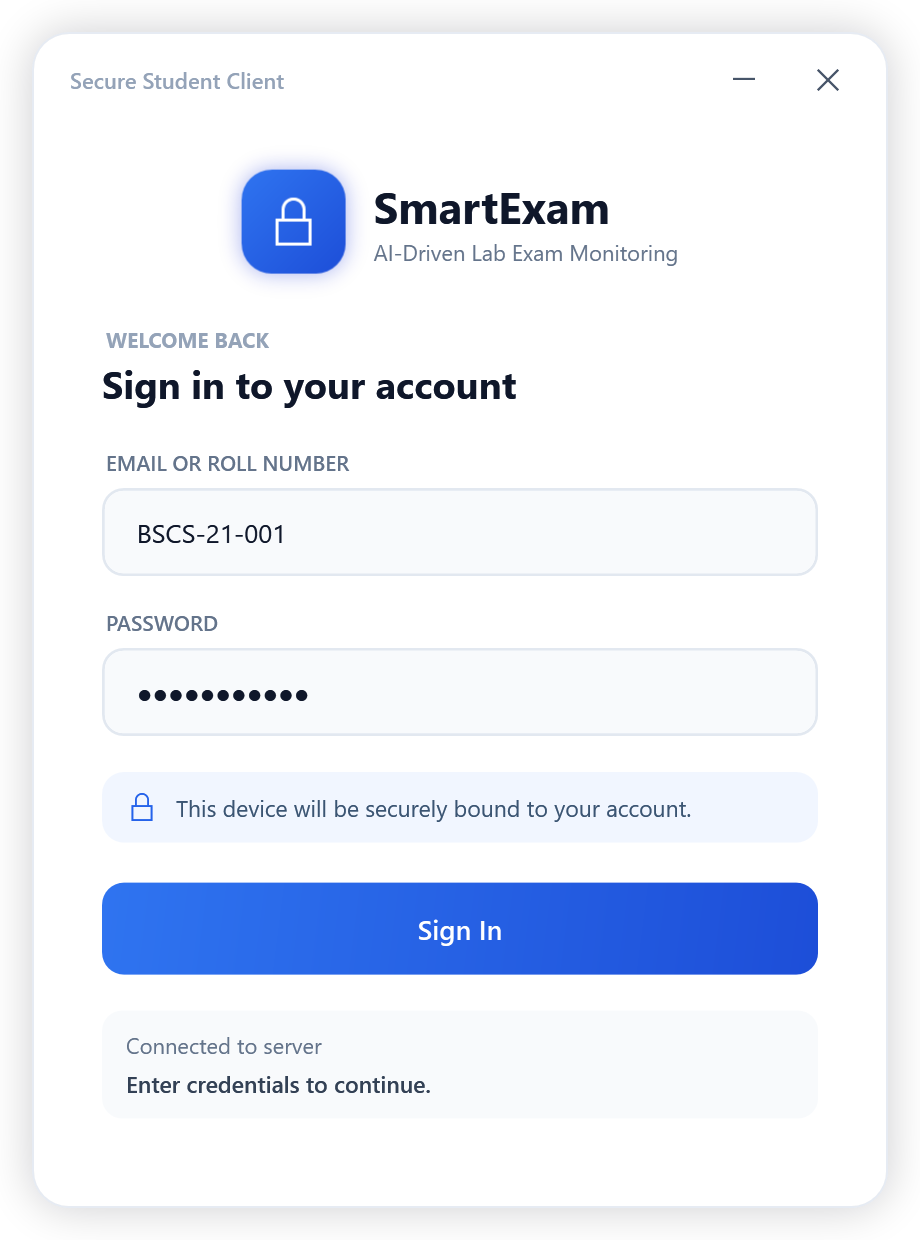
\includegraphics[width=\linewidth,height=0.9\textheight,keepaspectratio]{Figures/ui_student_login.png}
\caption{Desktop Client Login}
\label{fig:ui_student_login}
\end{figure}
\SoftBarrierN

The exam dashboard shows the student's current assigned exam with its instructions and permitted applications (Figure~\ref{fig:ui_student_diagnostics}); a side panel, not shown, gives the remaining time, lab, seat, attendance check-in and invigilator messages. An ineligible student still sees the exam, with \emph{Start Exam} disabled and the reason shown (FR3). In the figure, the blue header gives the exam title, its status (Active) and the teacher (Dr. Ahmed), and the permitted applications are \texttt{code.exe} and \texttt{codeblocks.exe}. In the \emph{System Check} list a green tick is a passed check, a dash is a skipped check and a red cross is a failed check with a \emph{Retry} button beside it. The dashboard runs the readiness checks (FR2): network, clock skew, screen capture, webcam, microphone, secure mode (monitors, remote session, virtual machine, keyboard hook) and disk space. This exam needs the webcam but not the microphone, so the microphone is skipped. Secure mode fails because a second monitor is attached, and since the exam requires the check (\texttt{RequireReadiness}), \emph{Start Exam} stays disabled until a passing check less than 30 minutes old exists.

\begin{figure}[tbp]
\centering
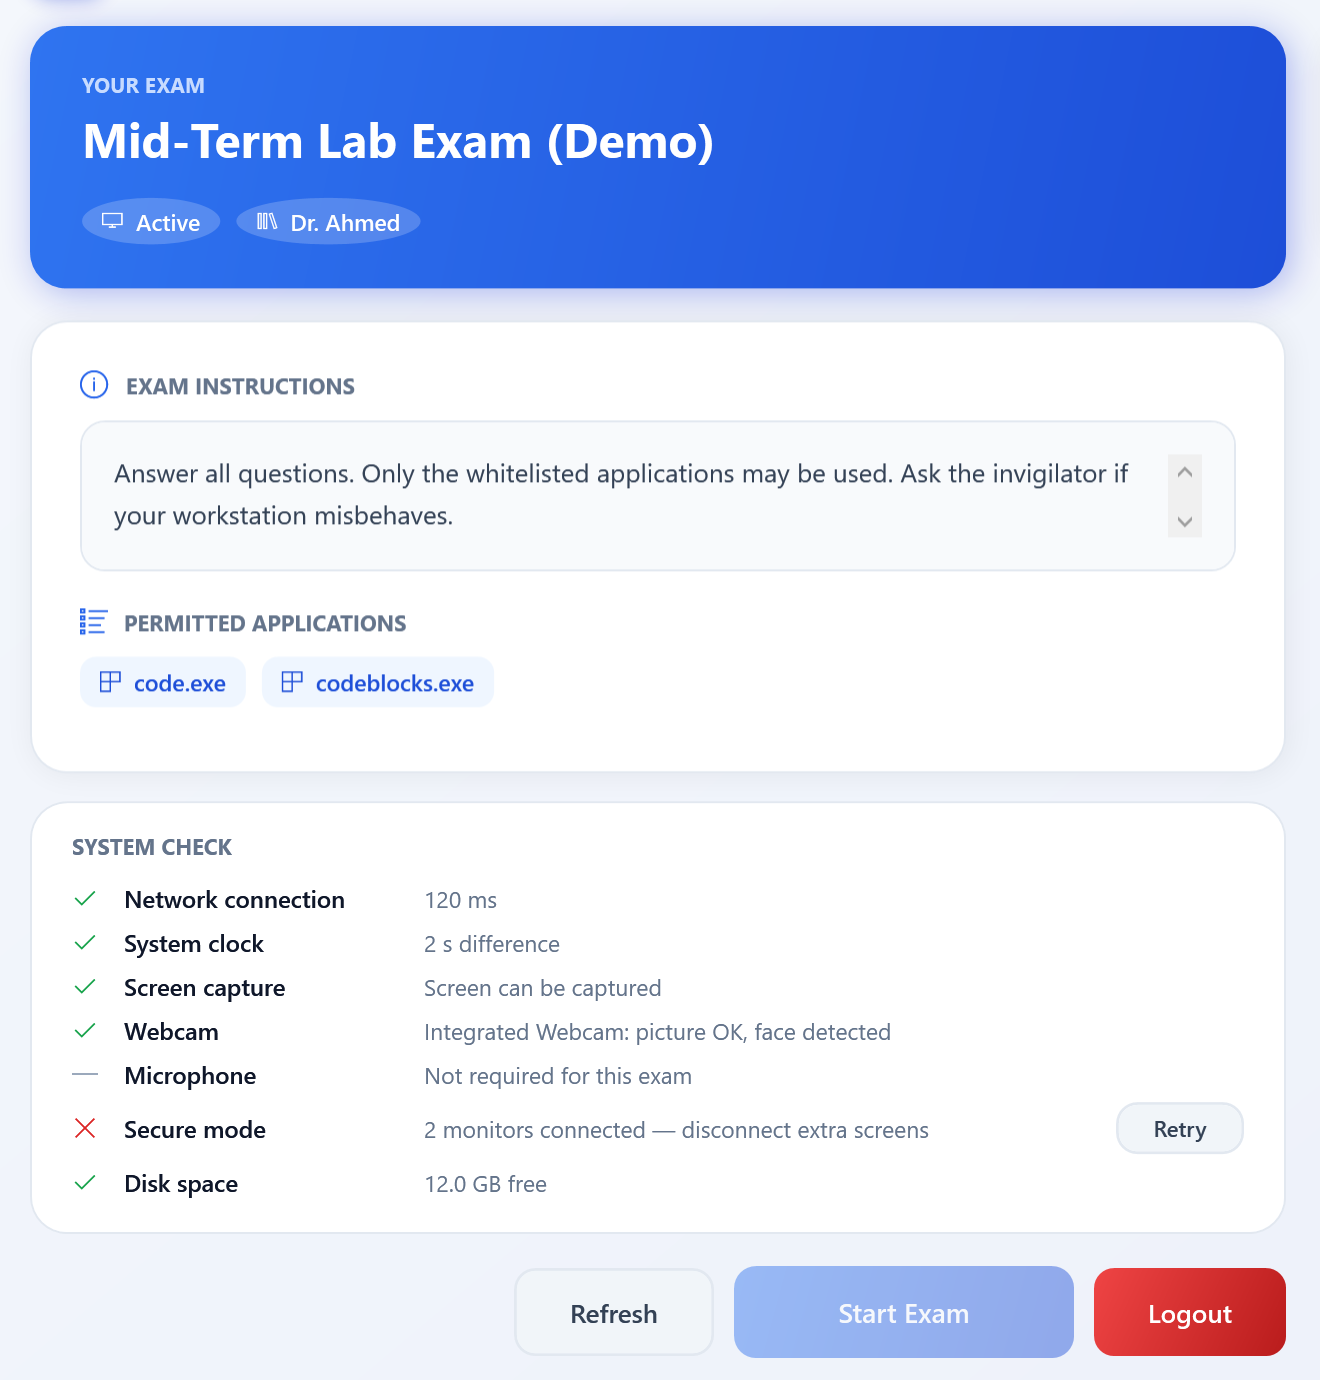
\includegraphics[width=\linewidth,height=472pt,keepaspectratio]{Figures/ui_student_diagnostics.png}
\caption{Exam Dashboard with Readiness Checks}
\label{fig:ui_student_diagnostics}
\end{figure}
\SoftBarrierN

The exam window (Figures~\ref{fig:ui_student_workspace} and~\ref{fig:ui_student_workspace_b}) opens maximised, borderless and topmost (FR4). A low-level keyboard hook blocks the Windows and menu keys, PrintScreen, Alt+Tab, Alt+F4, Alt+Esc, Ctrl+Esc and Ctrl+Shift+Esc, while guard services watch processes, the clipboard and newly mounted USB storage devices. The student picks a question from the list on the left and types the answer; coding answers go into a monospace text box. Every edit is written within about a second to an AES-256-GCM encrypted backup on disk and saved to the server 10~s after the first unsaved edit; saves made offline are queued and replayed (FR6). The footer shows the last save time.

The window is printed in two parts. Part~(a) is the left side panel: the exam title with the number of answered questions (2 of 3), the question list (1 Coding, 2 Theory, 3 Multiple Choice) with a green dot for each answered question, and the footer \emph{Saved 3:35:32 PM}; the empty middle of the panel is cut out. Part~(b) is the question area: the countdown timer (01:27:18) in the header, the type and marks of Question~1 (Coding, 20 marks), the C++ answer in the \emph{Your Code} box, and the \emph{Previous}, \emph{Next} and \emph{Submit Exam} buttons. So the student can always see how much is answered, how much time is left and when the work was last saved.

\begin{figure}[tbp]
\centering
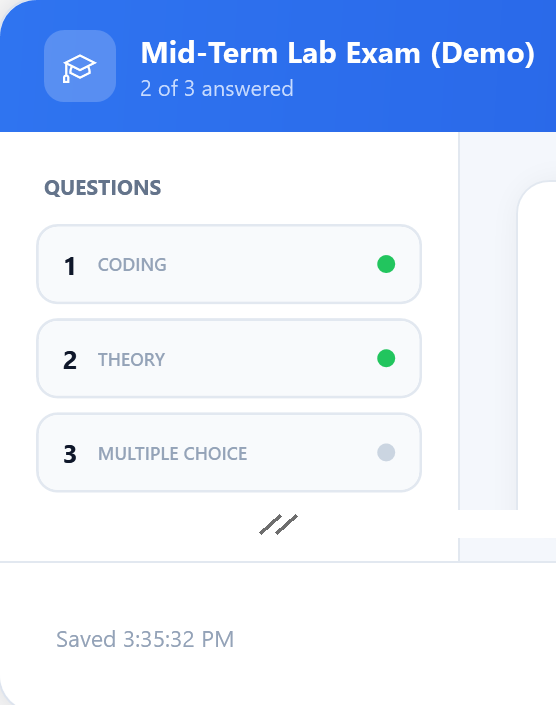
\includegraphics[width=0.5\linewidth]{Figures/ui_student_workspace_p1.png}
\caption{Desktop Exam Window (a): Question List and Save Status (Empty Middle Omitted)}
\label{fig:ui_student_workspace}
\end{figure}
\SoftBarrierN

\begin{figure}[tbp]
\centering
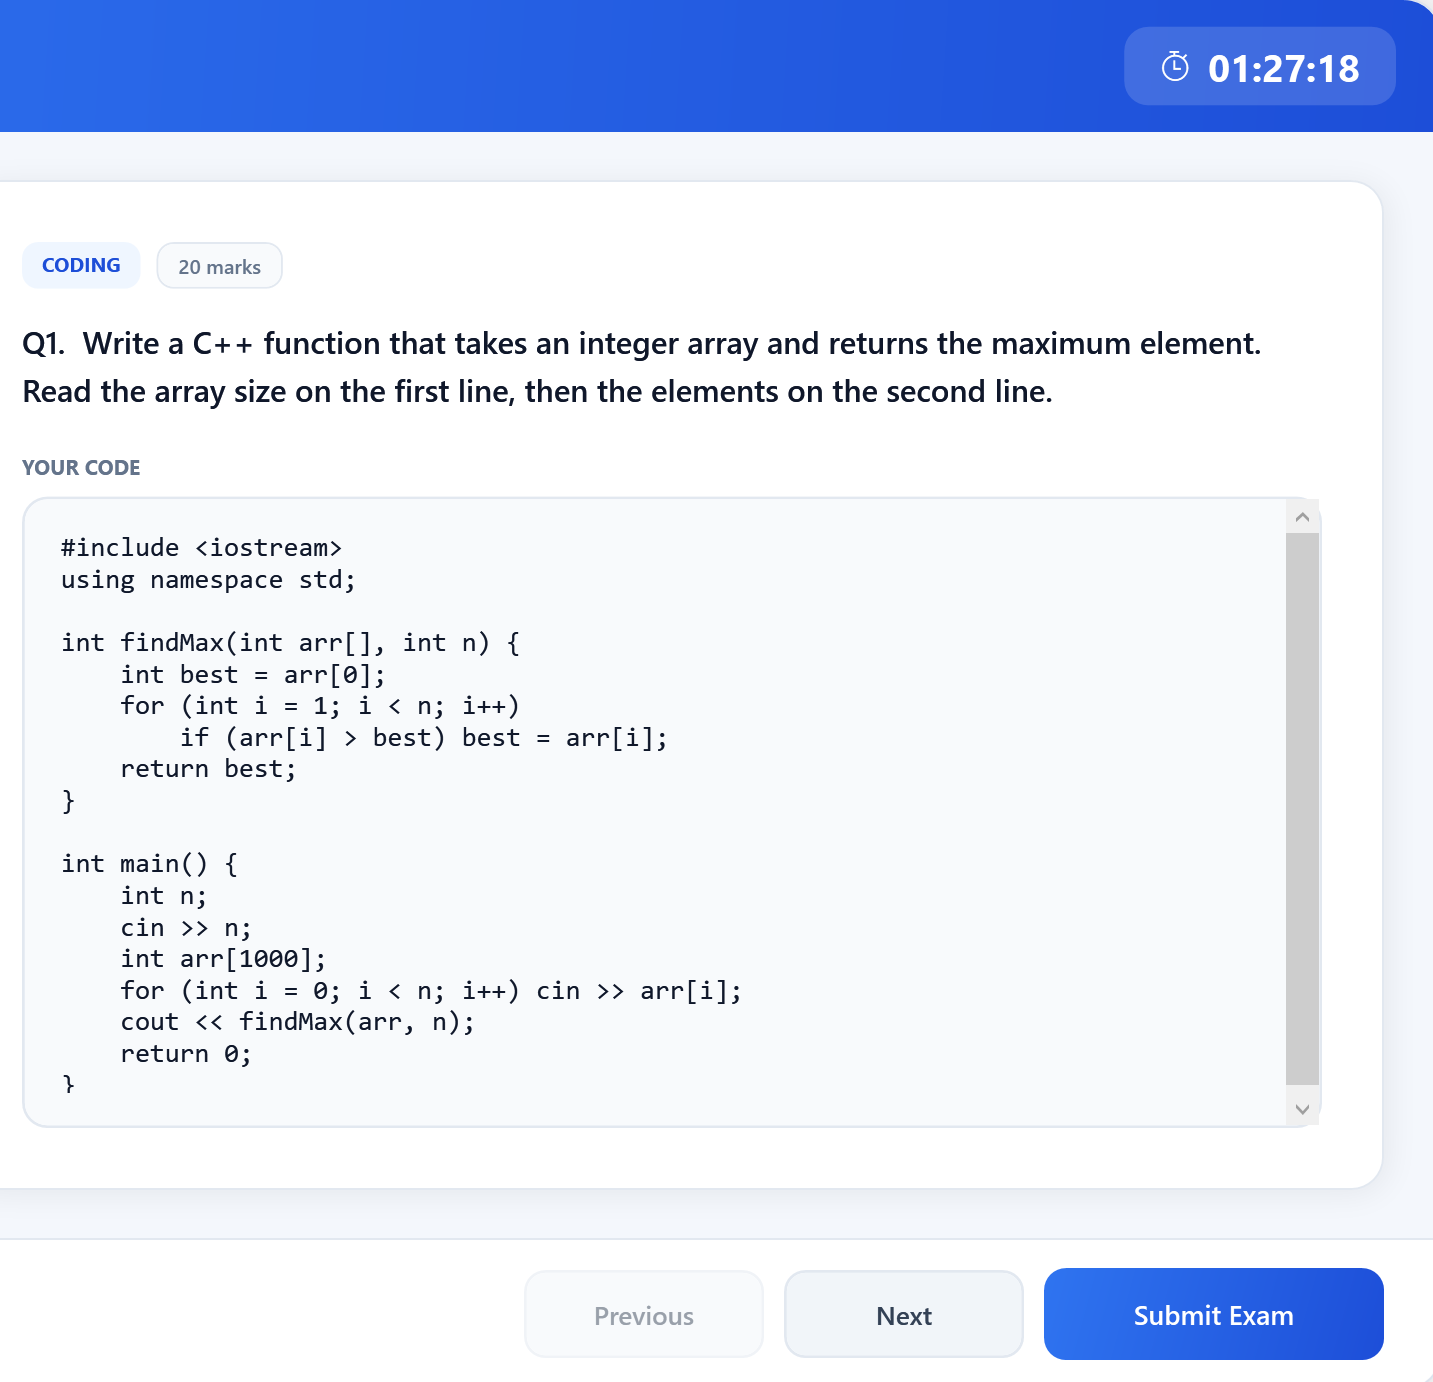
\includegraphics[width=\linewidth]{Figures/ui_student_workspace_p2.png}
\caption{Desktop Exam Window (b): Coding Question, Timer and Answer Box}
\label{fig:ui_student_workspace_b}
\end{figure}
\SoftBarrierN

A warning sent by an invigilator reaches the client in the reply to its next heartbeat (every 10~s) and appears as a banner between the window header and the question (Figure~\ref{fig:ui_student_warning}, the warning sent in Figure~\ref{fig:ui_live_timeline}). The banner shows the title \emph{Proctor Warning} with the time it was sent (15:35), the invigilator's message and an \emph{Acknowledge} button; the empty middle of the wide banner is cut out. The banner stays until the student acknowledges it, further warnings wait in a queue and are shown one by one, and the student's \emph{Acknowledge} is written to the audit log (FR10).

\begin{figure}[tbp]
\centering

\includegraphics[width=\linewidth]{Figures/ui_student_warning_banner.png}
\caption{Invigilator Warning Banner in the Exam Window (Empty Middle Omitted)}
\label{fig:ui_student_warning}
\end{figure}
\SoftBarrierN

\subsection{Exam Setup}
The teacher dashboard (Figure~\ref{fig:ui_teacher_dashboard}) counts the teacher's exams, the running ones and the ended exams waiting for grade review. It lists scheduled exams, including the seeded practice exam, which stays open for a week, with \emph{Manage}, \emph{Edit} and \emph{Delete}, and links each ended exam to \emph{Review Grades}. In the figure, Dr. Ahmed has six exams, one running now and three waiting for review. The left list holds the two scheduled exams, the practice exam (tagged \emph{Practice}) and the End-Term Lab Exam (tagged \emph{Ready}), and the right panel lists the three ended Data Structures exams. The page tells the teacher at a glance what is coming next and what still needs grading.

\begin{figure}[tbp]
\centering
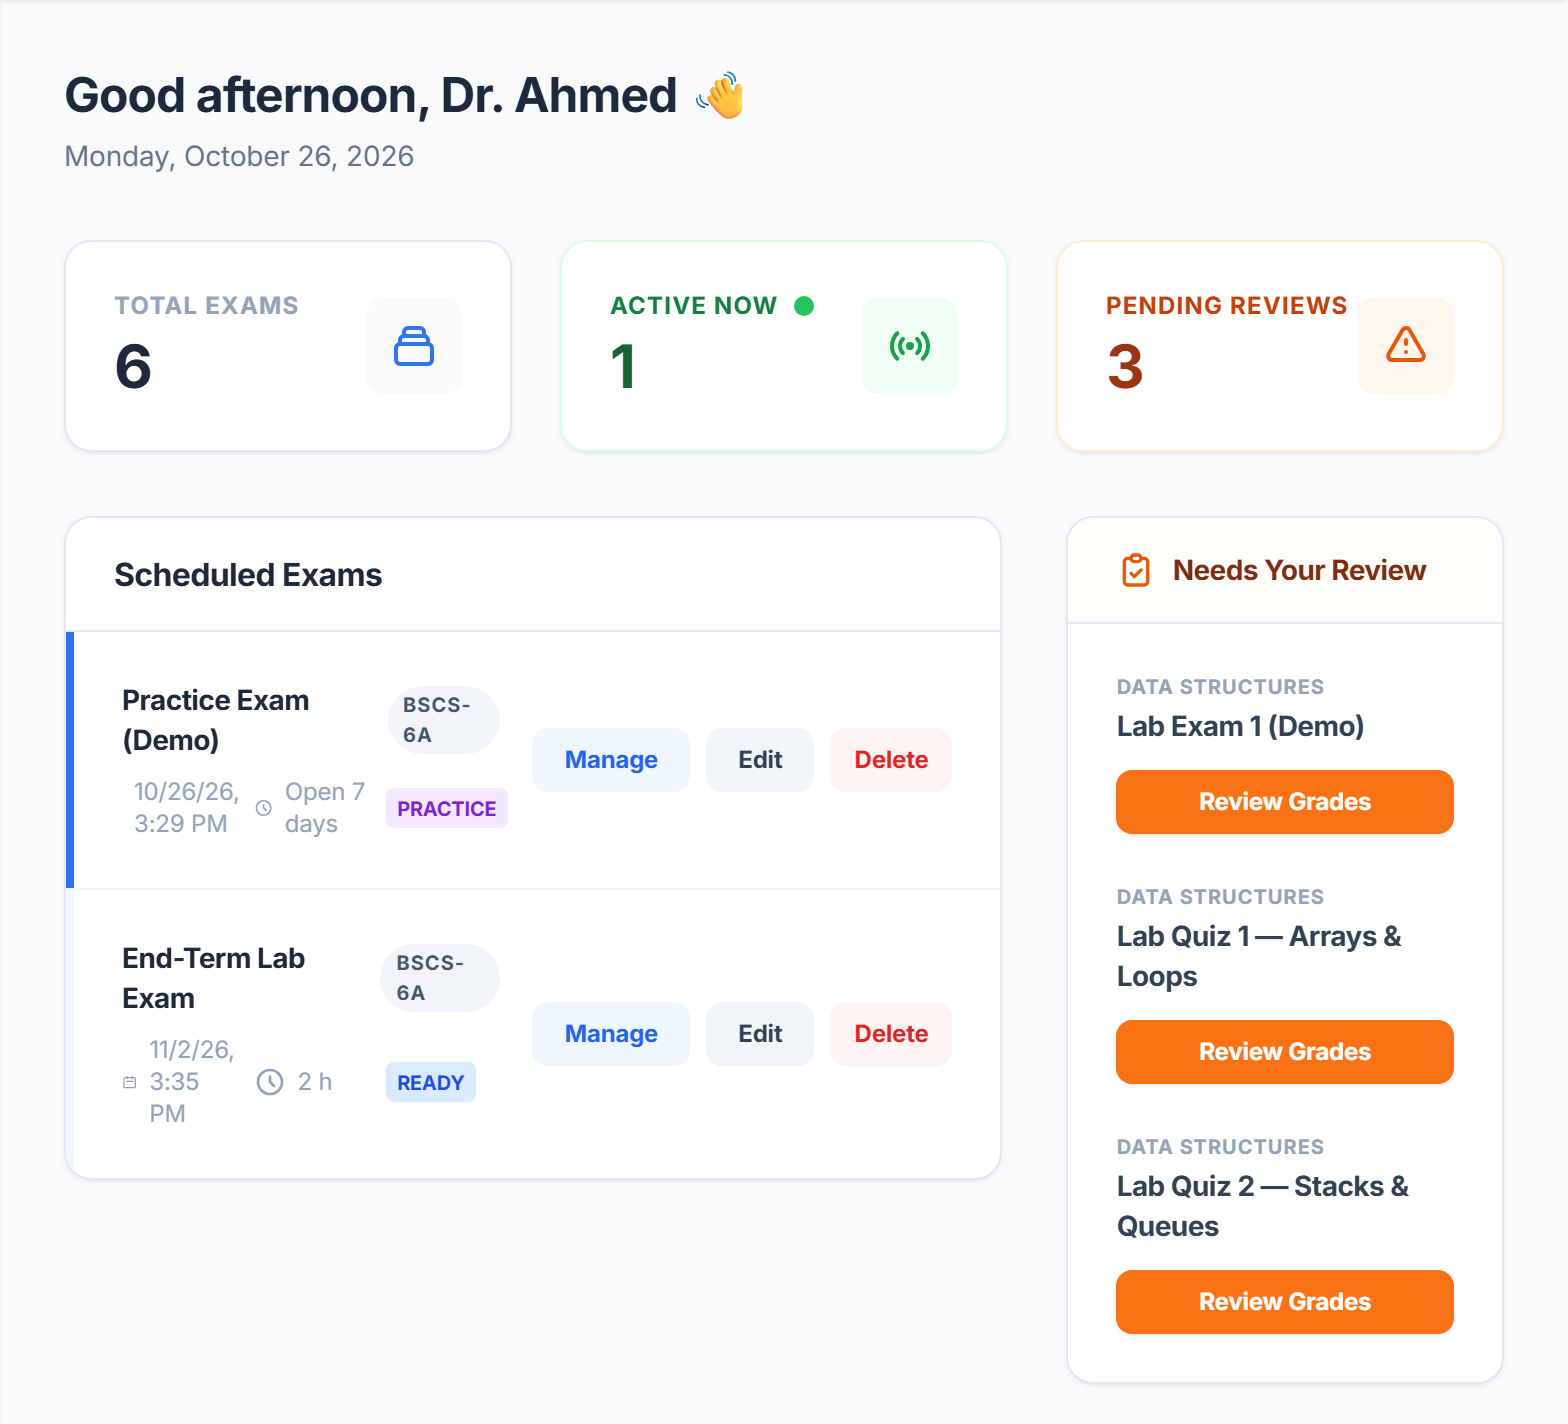
\includegraphics[width=\linewidth,height=410pt,keepaspectratio]{Figures/ui_teacher_dashboard.png}
\caption{Teacher Dashboard}
\label{fig:ui_teacher_dashboard}
\end{figure}
\SoftBarrierN

\begin{figure}[p]
\centering
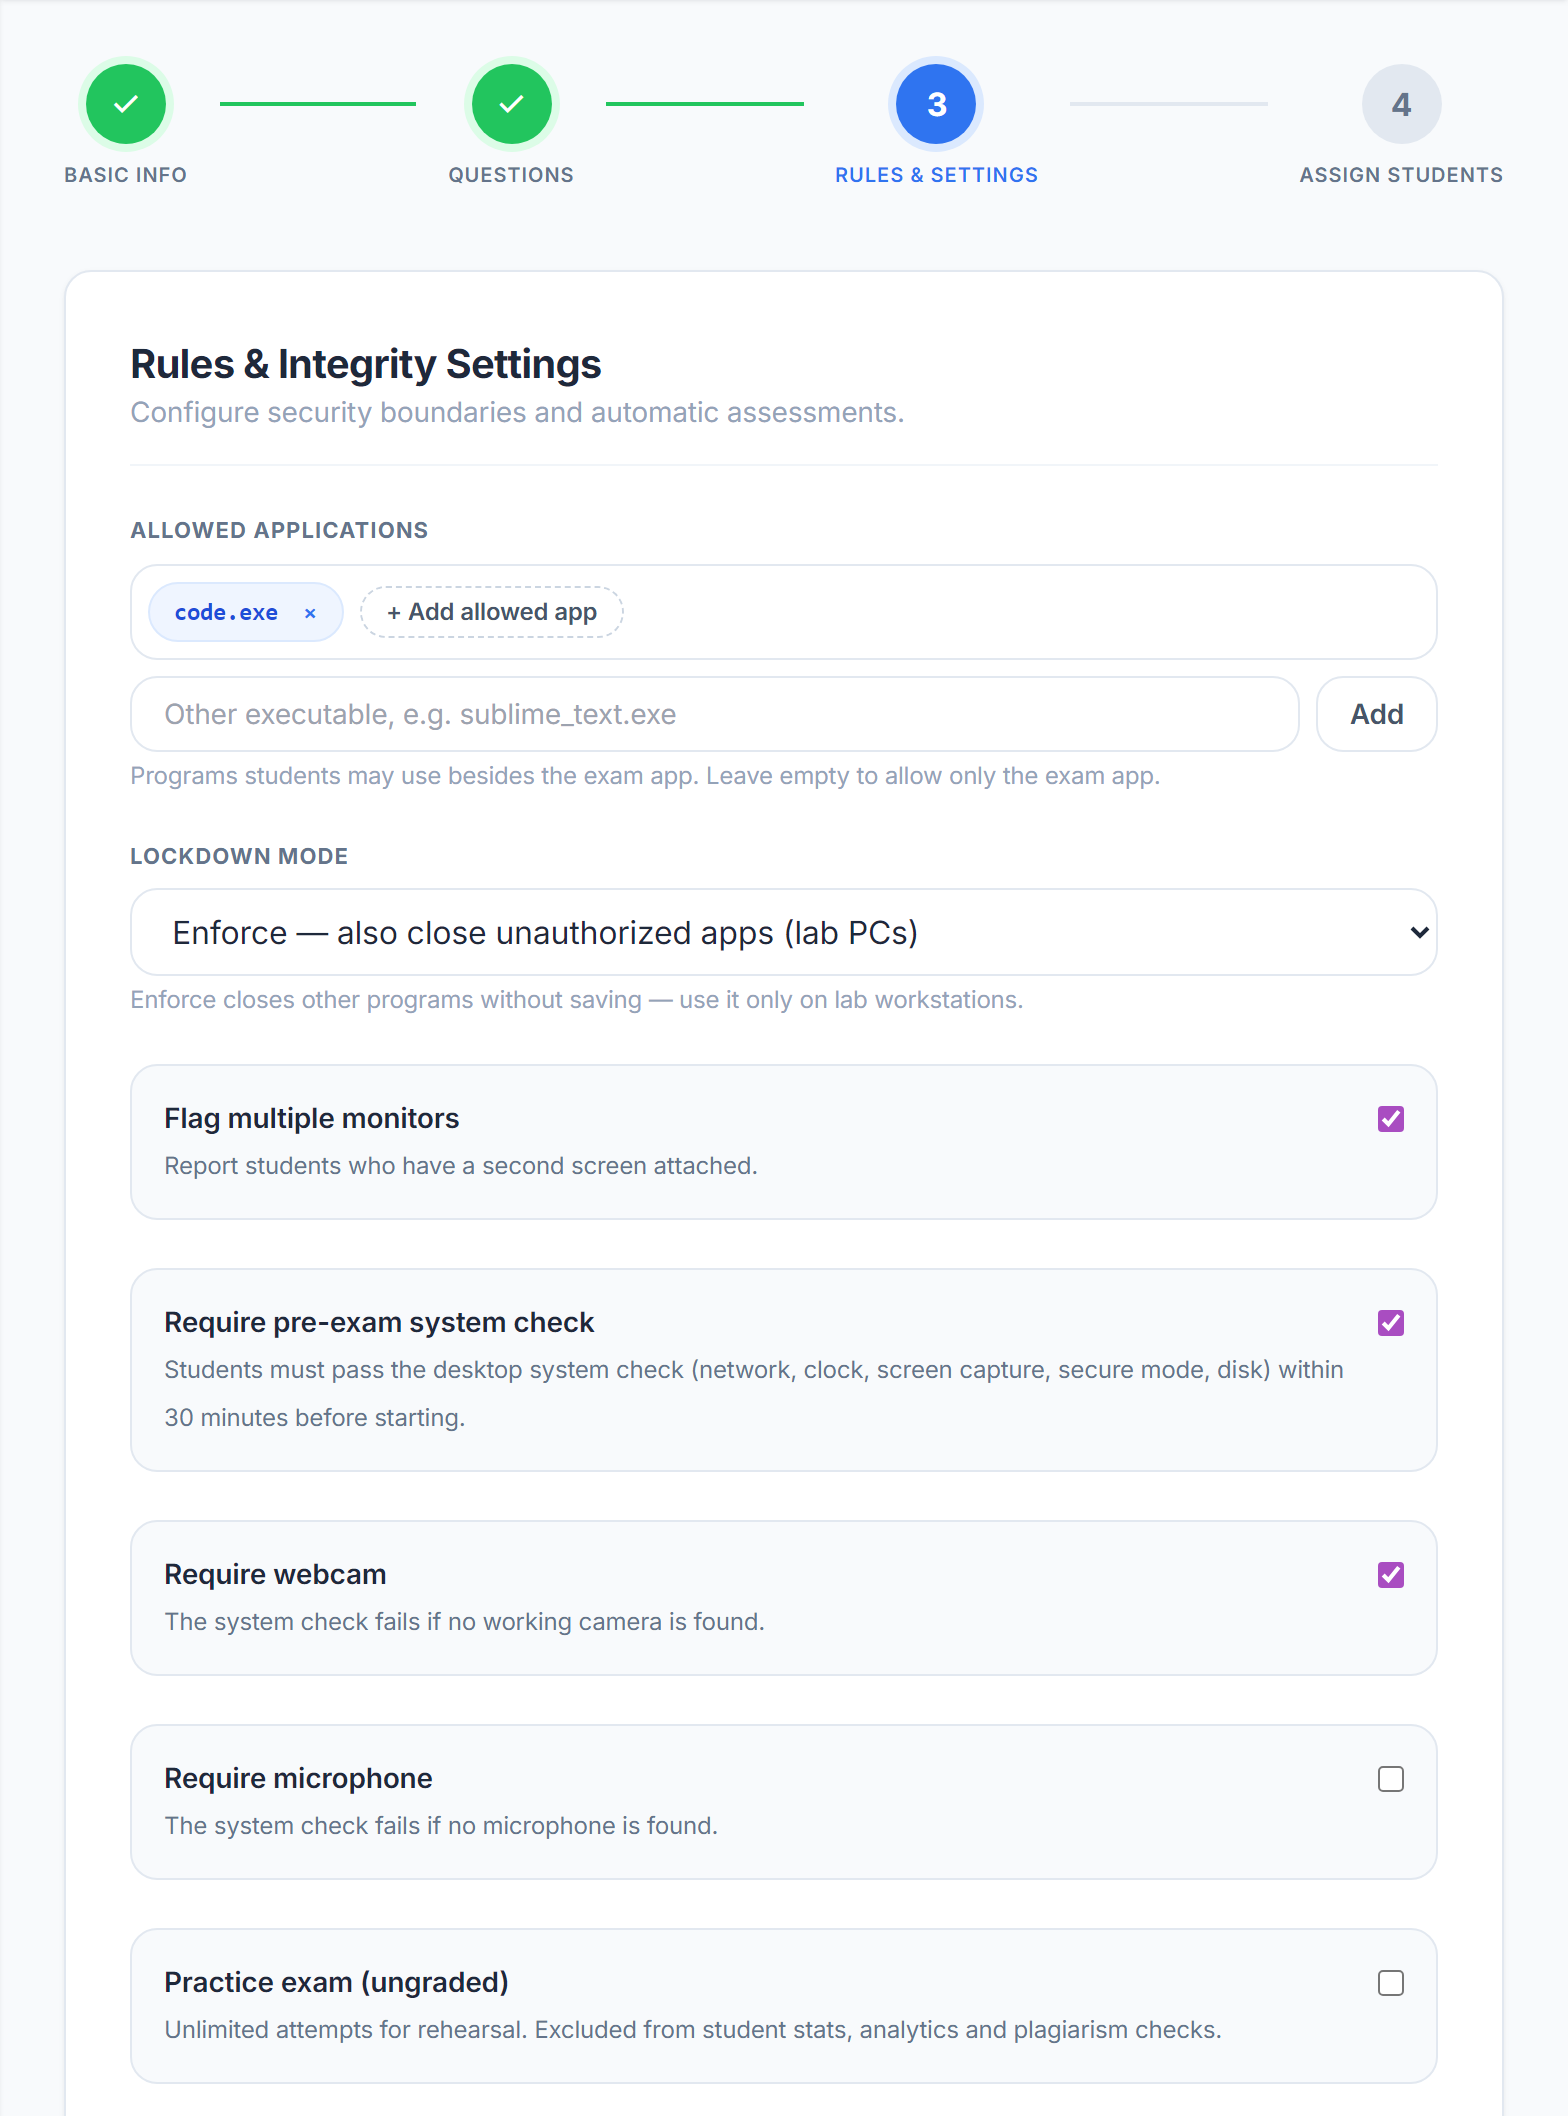
\includegraphics[width=\linewidth,height=628pt,keepaspectratio]{Figures/ui_create_exam_rules.png}
\caption{Create-Exam Wizard, Rules Step: Integrity Switches}
\label{fig:ui_create_exam_rules}
\end{figure}
\SoftBarrierN

A four-step wizard creates an exam: basic information, questions (MCQ, coding with test cases, theory), rules, and students (FR8). Step~3 holds the integrity rules: allowed applications, lockdown mode (Off, Report, Enforce), the multi-monitor flag, the required system check, webcam and microphone, and the practice-exam switch (Figure~\ref{fig:ui_create_exam_rules}); then early join, minimum attendance, the screenshot and webcam intervals, seat enforcement, AI evaluation and the plagiarism threshold (Figure~\ref{fig:ui_create_exam_rules_more}).

In Figure~\ref{fig:ui_create_exam_rules} the step bar shows that \emph{Basic Info} and \emph{Questions} are done and \emph{Rules \& Settings} is the current step. In this example only \texttt{code.exe} is allowed, and the lockdown mode is Enforce, which closes other programs without saving, so the hint says to use it only on lab PCs. The multi-monitor flag, the system check and the webcam are switched on, while the microphone and the practice-exam switch are off.

Figure~\ref{fig:ui_create_exam_rules_more} shows the lower half of the same step. Here early join is 0 minutes, the minimum attendance is 75\,\%, both capture intervals are 60~s, seat enforcement and AI evaluation are on, and the plagiarism threshold is 70\,\%. The hint under the screenshot interval explains that each gap is randomised by $\pm$50\,\% (30--90~s for 60~s) and that a violation causes an immediate capture, so a student cannot predict when the next capture comes.

\begin{figure}[tbp]
\centering
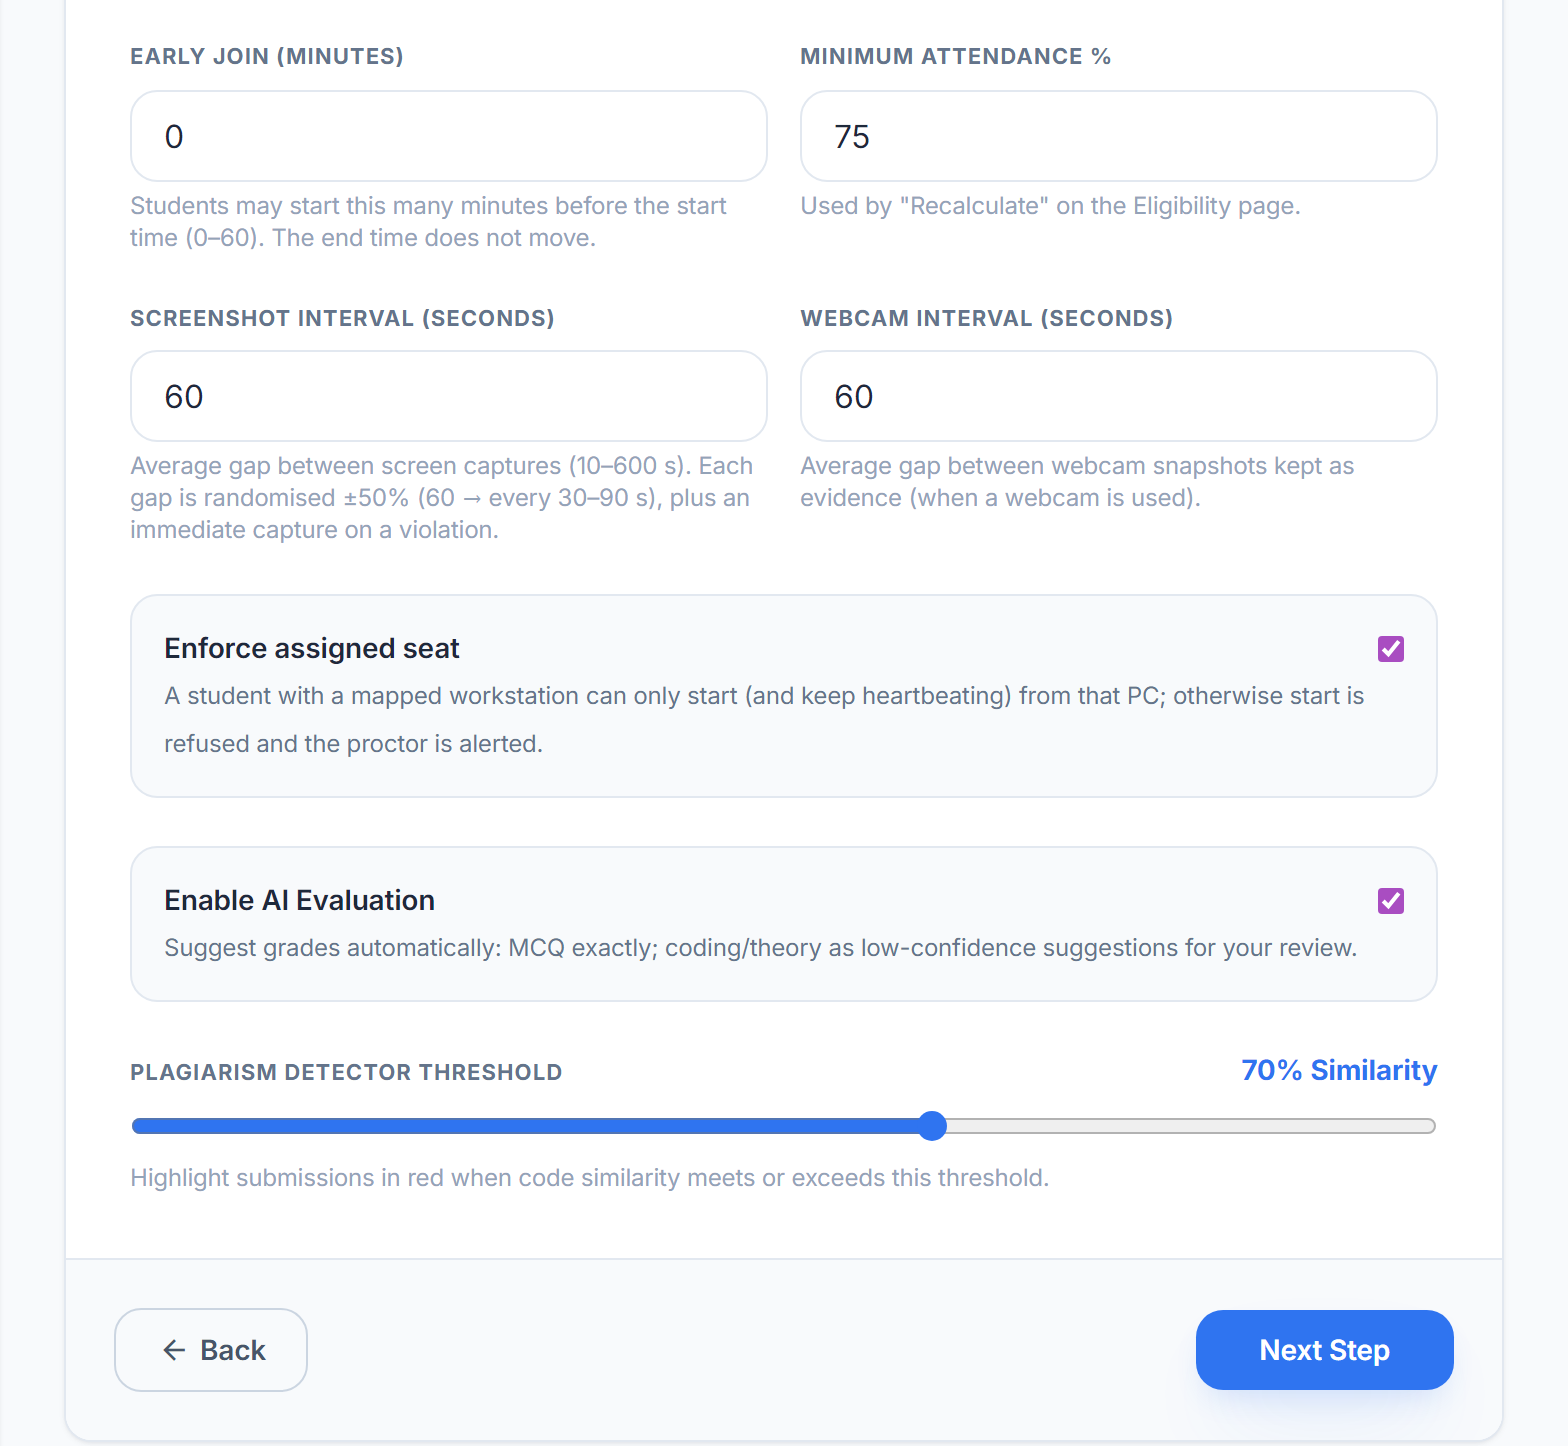
\includegraphics[width=\linewidth,height=416pt,keepaspectratio]{Figures/ui_create_exam_rules_more.png}
\caption{Create-Exam Wizard, Rules Step: Intervals, Seat, AI and Plagiarism Settings}
\label{fig:ui_create_exam_rules_more}
\end{figure}
\SoftBarrierN

On the eligibility page (Figure~\ref{fig:ui_eligibility}) the teacher uploads an attendance CSV (comma-separated values) file and clicks \emph{Recalculate}; students below the exam's minimum attendance become ineligible (FR9), as Hamza Iqbal (60\,\%) is here. Each row shows where its decision came from (\emph{Attendance} in the figure); a saved toggle for a single student becomes a \emph{Manual} override, which survives recalculation and is audited. The same page maps each student to a workstation (seat) and assigns invigilators, who then see only this exam.

The page is printed in two parts that show the same six rows in the same order. Part~(a) (Figure~\ref{fig:ui_eligibility}) holds the exam selector with its minimum attendance of 75\,\%, the \emph{Invigilators} card with Mr. Bilal assigned, and each student's name with a seat drop-down (R1C1 to R2C2 in Lab~A). Part~(b) (Figure~\ref{fig:ui_eligibility_b}) holds the buttons \emph{Upload Attendance}, \emph{Recalculate}, \emph{Mark All Eligible} and \emph{Mark All Ineligible}, the invigilator picker, and for each row the system check, the attendance, the eligibility switch with its source tag and the reason. Five students have 77.5--95\,\% attendance and are eligible. The last row is Hamza Iqbal: with 60\,\% (24 of 40 classes) his switch is off and the reason \emph{Attendance 60\% < 75\%} is shown in red. A green tick in the system-check column means a passing check less than 30 minutes old; Hamza has a dash because no check is recorded for him.

\begin{figure}[tbp]
\centering
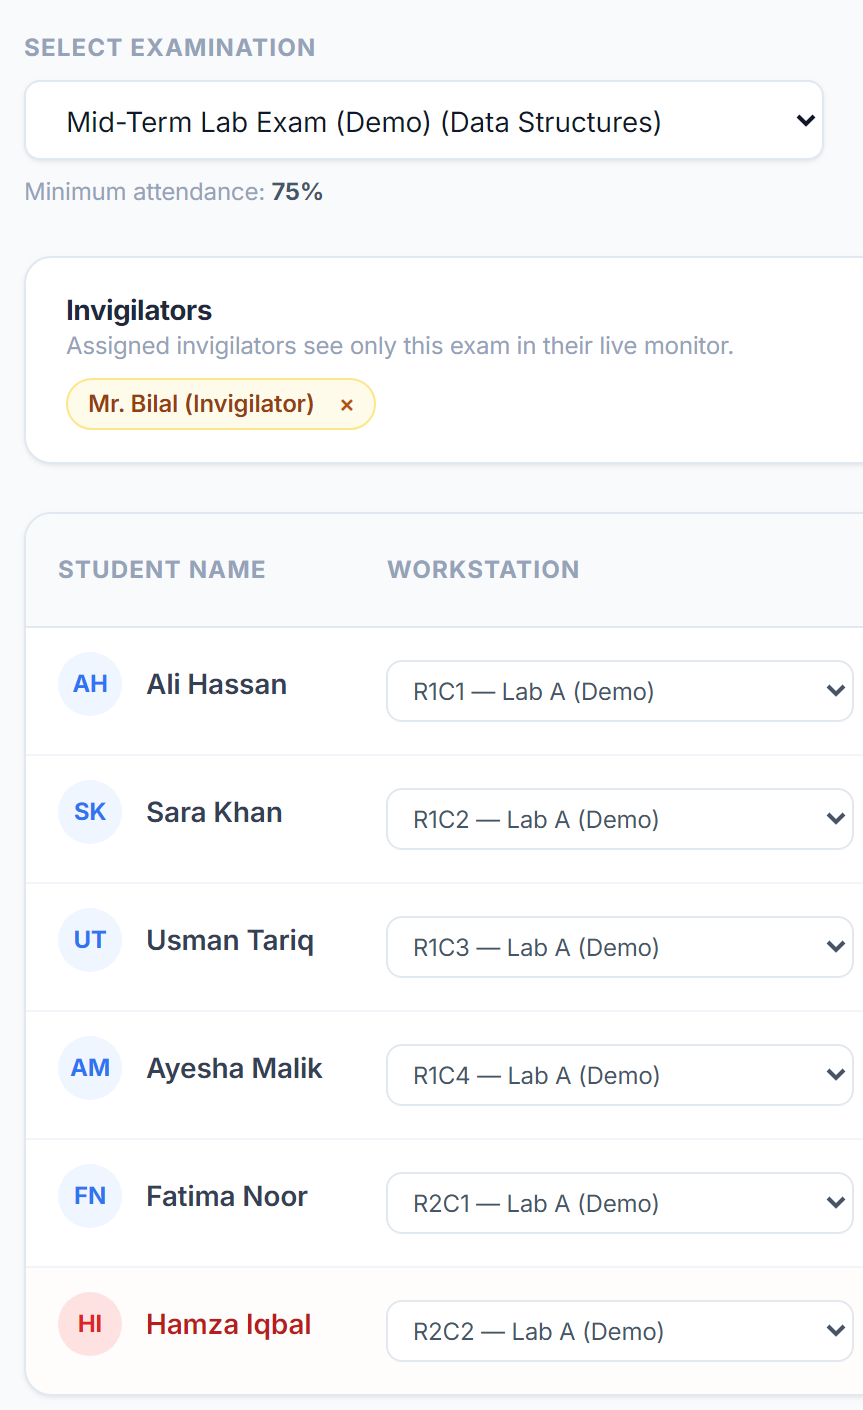
\includegraphics[width=0.72\linewidth]{Figures/ui_eligibility_p1.png}
\caption{Eligibility, Seats and Invigilators (a): Exam, Invigilators and Seats (Email Column Omitted)}
\label{fig:ui_eligibility}
\end{figure}
\SoftBarrierN

\begin{figure}[tbp]
\centering
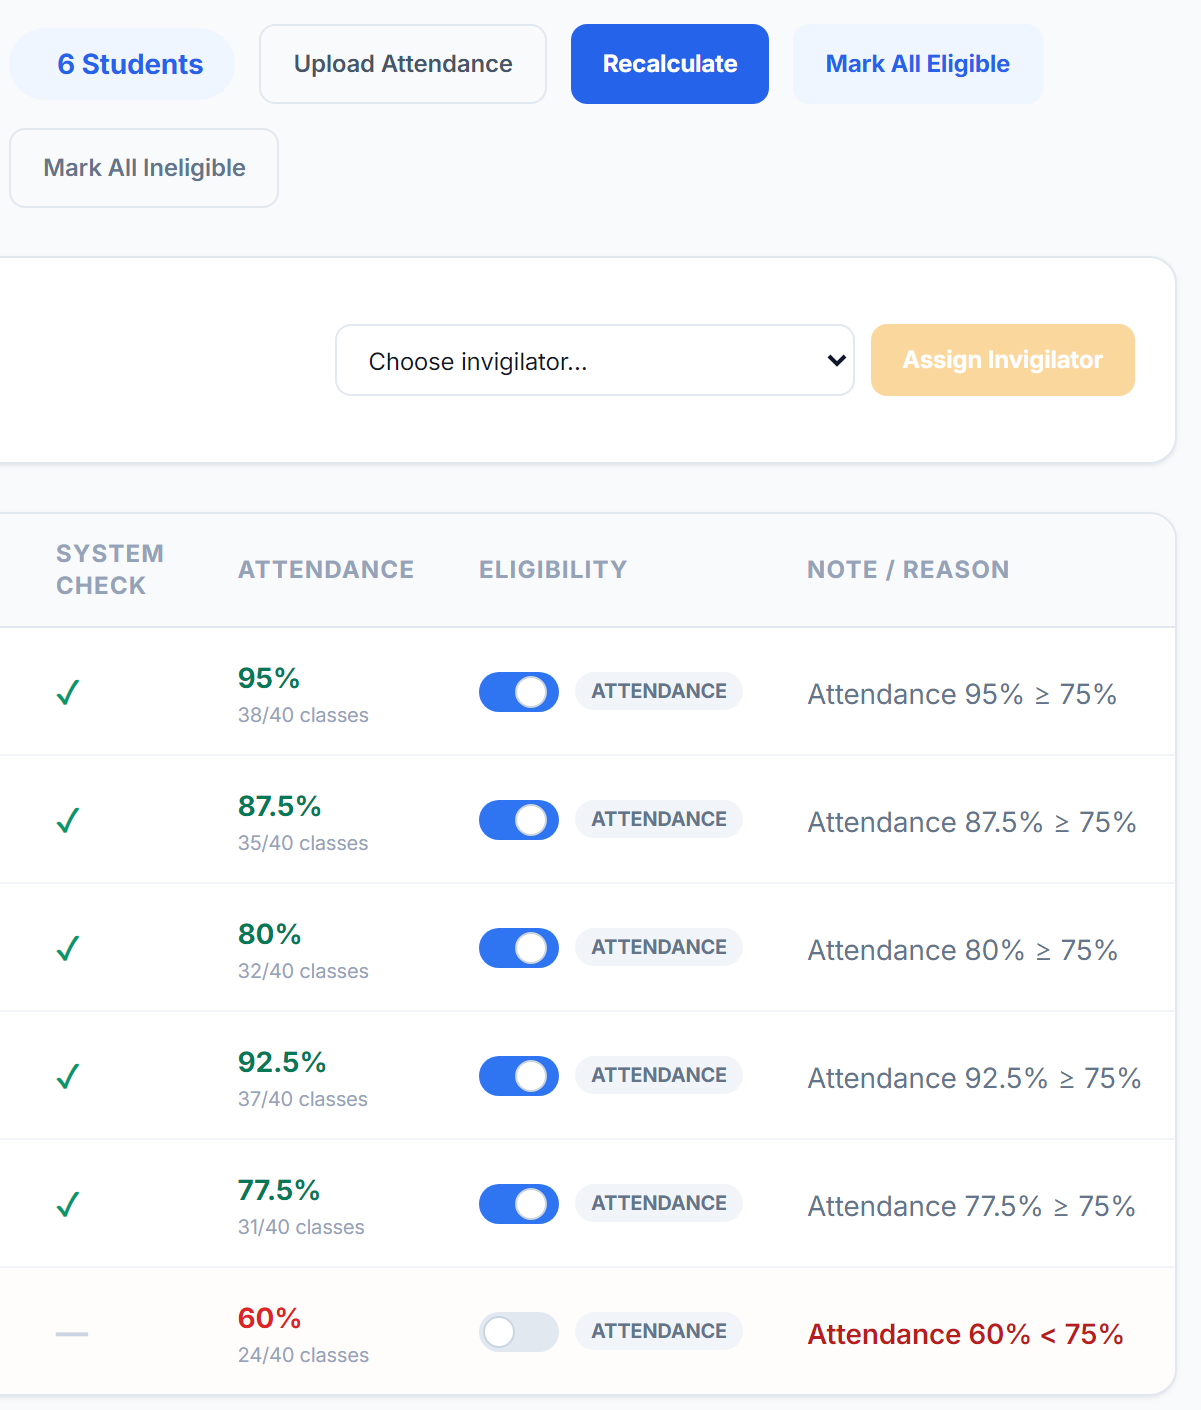
\includegraphics[width=\linewidth]{Figures/ui_eligibility_p2.png}
\caption{Eligibility, Seats and Invigilators (b): Attendance and Eligibility (Same Rows as Part (a))}
\label{fig:ui_eligibility_b}
\end{figure}
\SoftBarrierN

\subsection{Live Invigilation}\suppressfloats[t]
SignalR carries live updates between the API and the web dashboard; the desktop client uses REST only and receives invigilator warnings, extra time, unlocks and force-submits in the reply to its next heartbeat (every 10~s). The client sends heartbeats, event batches and screen captures to \url{/api/monitoring}, and the server pushes each update to the live monitor (Figures~\ref{fig:ui_teacher_live_monitoring} to~\ref{fig:ui_teacher_live_monitoring_b}) over the hub \url{/hubs/monitoring} (FR5, FR10). Through \texttt{ExamProctors}, invigilators see only the exams assigned to them. The header of the live monitor (Figure~\ref{fig:ui_teacher_live_monitoring}) names the current exam with its course tag and an exam selector, and shows the remaining time (01:27:10) on the right. It also shows that four students are still sitting (Ali Hassan has already submitted) and gives the \emph{Extend Time} and \emph{Force End Exam} buttons, which act on the whole exam.

\begin{figure}[tbp]
\centering
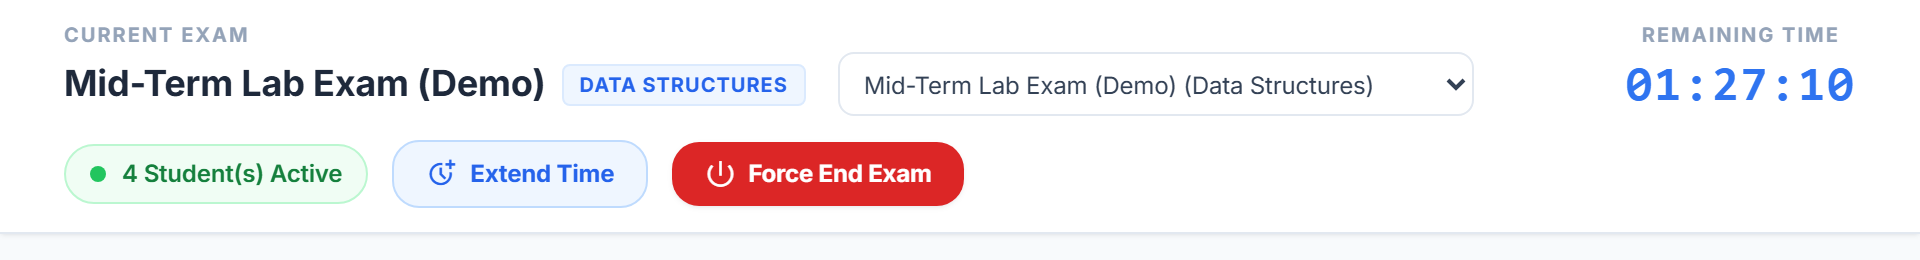
\includegraphics[width=\linewidth]{Figures/ui_live_monitor_a_p1.png}
\caption{Live Monitor (a): Header with Remaining Time and Exam Controls}
\label{fig:ui_teacher_live_monitoring}
\end{figure}
\SoftBarrierN

Below the header each student has a tile (Figures~\ref{fig:ui_teacher_live_monitoring_tiles} to~\ref{fig:ui_teacher_live_monitoring_b}). Each tile shows the student's seat and PC with the Windows user, readiness, latest capture, latest alert and progress as answered questions with a bar. The heart icon and the border colour give the status: the classifier level as Stable (Normal), Warning, Suspicious or Critical (Violation); a client silent for 30~s is shown as Disconnected, and a finished session as Submitted, Force submitted or Timed out. The captures are small thumbnails, and their text is not meant to be read at this size.

Ali Hassan (seat R1C1) has answered all three questions and submitted, and Sara Khan (R1C2) is a Warning with one alert, \emph{Blocked keys}, for her blocked Alt+Tab (Figure~\ref{fig:ui_teacher_live_monitoring_tiles}). Usman Tariq (R1C3) is Critical with two alerts and one incident (Figure~\ref{fig:ui_teacher_live_monitoring_tile3}): he opened Chrome, which is not on the allowed list, and Enforce mode closed it, as the line \emph{Unauthorized app closed: chrome (Killed)} says; his capture shows a browser search. In the second row (Figure~\ref{fig:ui_teacher_live_monitoring_b}), Ayesha Malik's phone in view makes her Suspicious, and Fatima Noor is Stable with an \emph{Idle 9m} badge, which means no keyboard or mouse input on her PC for nine minutes.

\begin{figure}[tbp]
\centering
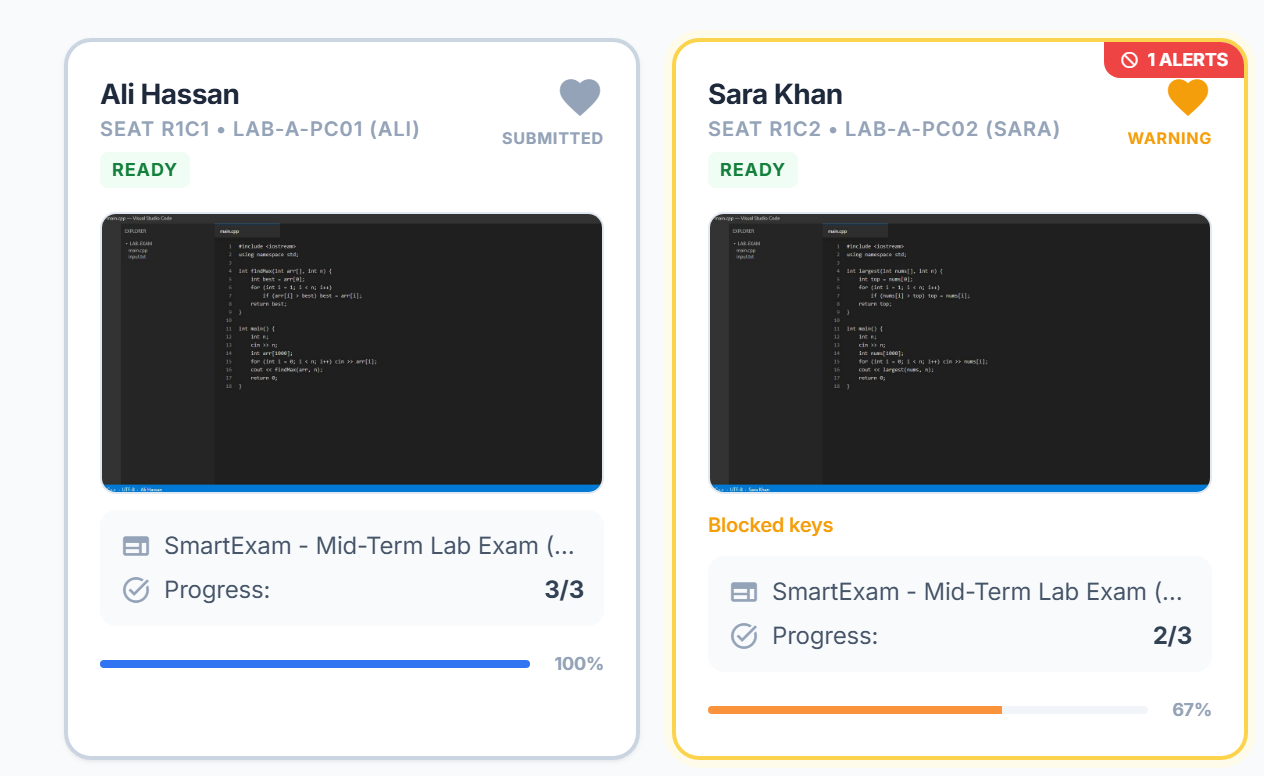
\includegraphics[width=\linewidth]{Figures/ui_live_monitor_a_p2.png}
\caption{Live Monitor (b): First Row, Tiles of Ali Hassan and Sara Khan}
\label{fig:ui_teacher_live_monitoring_tiles}
\end{figure}
\SoftBarrierN

\begin{figure}[tbp]
\centering
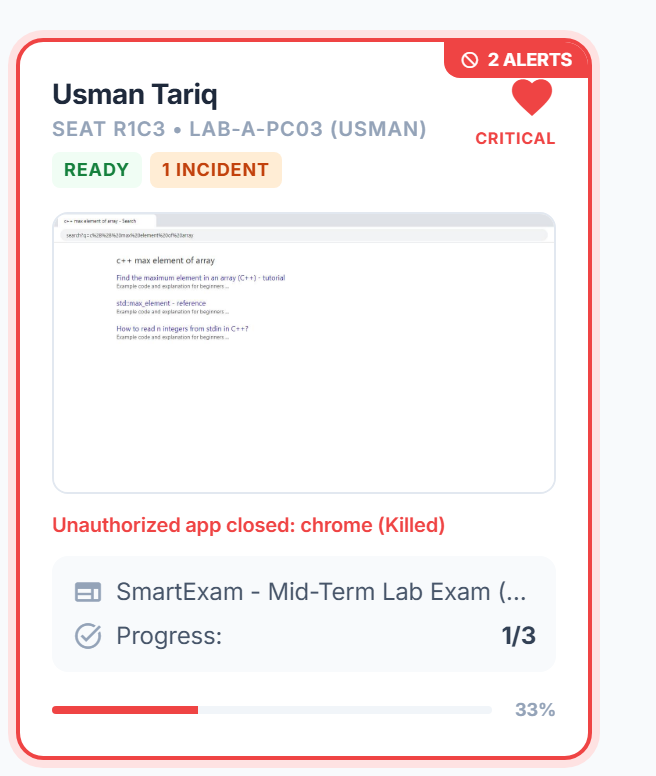
\includegraphics[width=0.52\linewidth]{Figures/ui_live_monitor_a_p3.png}
\caption{Live Monitor (c): First Row, Tile of Usman Tariq}
\label{fig:ui_teacher_live_monitoring_tile3}
\end{figure}
\SoftBarrierN

\begin{figure}[tbp]
\centering
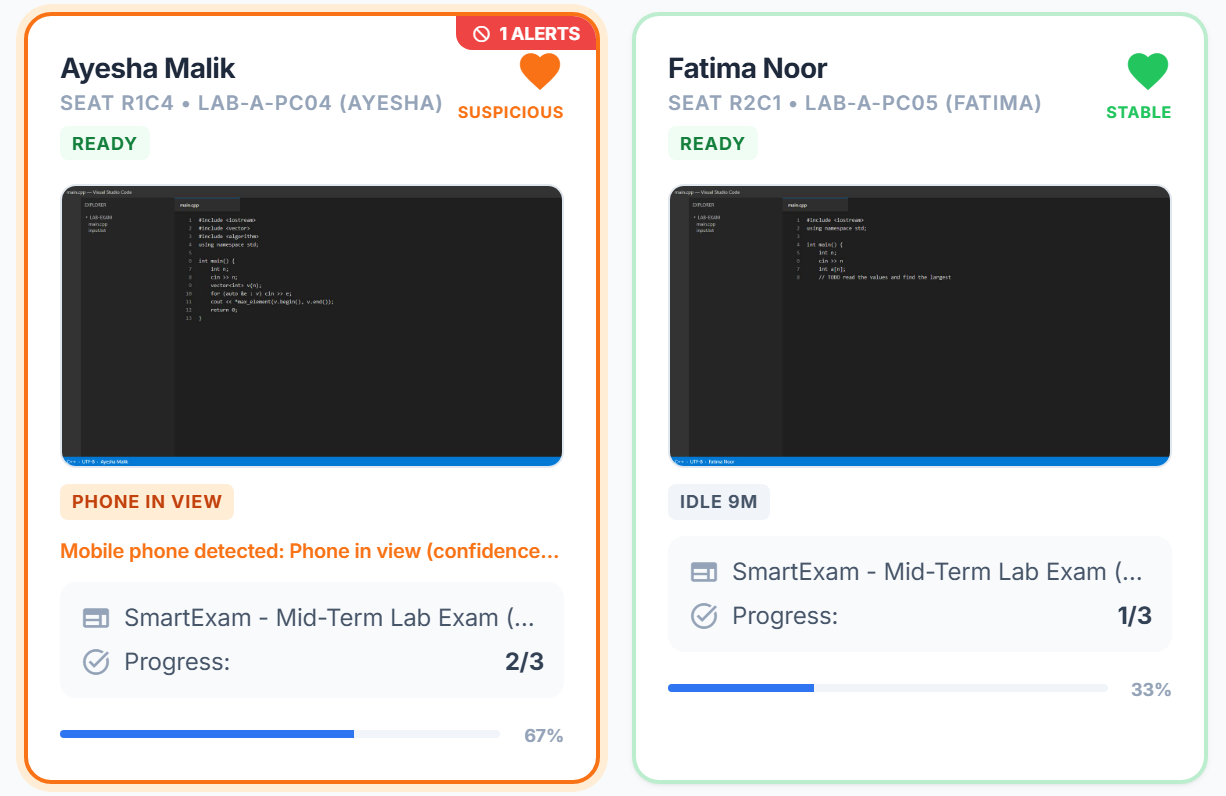
\includegraphics[width=\linewidth,height=293pt,keepaspectratio]{Figures/ui_live_monitor_b.png}
\caption{Live Monitor (d): Second Row of Tiles}
\label{fig:ui_teacher_live_monitoring_b}
\end{figure}
\SoftBarrierN

Clicking a tile opens the student drawer, here for Usman Tariq (Figure~\ref{fig:ui_live_drawer}). Its top gives the seat, the PC and the Windows user with the number of active alerts and open incidents. Below are the latest captures (the newer one, outlined in orange, shows the browser search), the readiness result (all seven checks passed on LAB-A-PC03 at 3:35:26~PM) and the applications seen on the PC, where Chrome is struck through because it is no longer running. So the invigilator sees all the evidence for one student in one place before acting.

\begin{figure}[p]
\centering
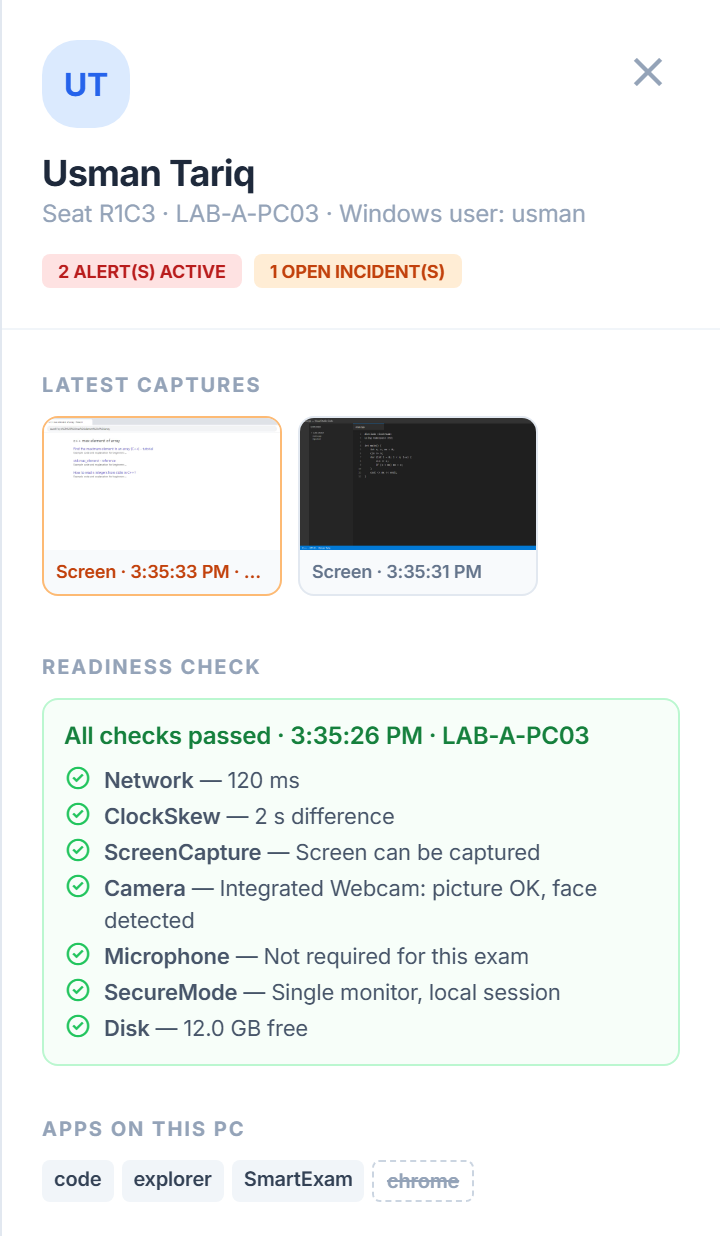
\includegraphics[width=\linewidth,height=628pt,keepaspectratio]{Figures/ui_live_drawer_evidence.png}
\caption{Student Drawer (a): Evidence}
\label{fig:ui_live_drawer}
\end{figure}
\SoftBarrierN

From the action panel (Figure~\ref{fig:ui_live_drawer_b}) the invigilator sends a warning, records an incident, unlocks the PC for five minutes with a short reason (the server allows 1--30 minutes), grants extra time or force-submits the session (FR10). The green line \emph{Warning Message Sent} confirms that the warning was sent. Force-submit is the red button because it ends the student's attempt; like the other actions, it reaches the desktop client in the reply to its next heartbeat.

\begin{figure}[tbp]
\centering
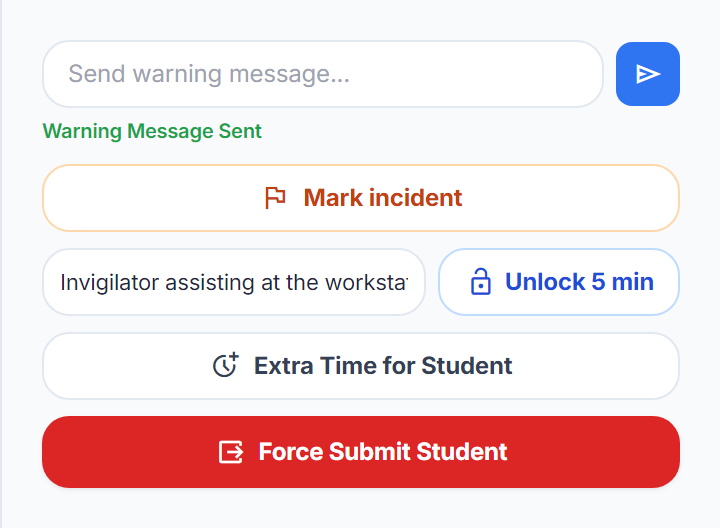
\includegraphics[width=0.55\linewidth]{Figures/ui_live_drawer_actions.png}
\caption{Student Drawer (b): Actions}
\label{fig:ui_live_drawer_b}
\end{figure}
\SoftBarrierN

Further down (Figure~\ref{fig:ui_live_timeline}) are the open incidents, with \emph{Escalate} and \emph{Mark resolved}, and the activity timeline. The incident card shows its severity (High), its status (Open), the note and who recorded it (Dr. Ahmed). The timeline lists the events newest first: Chrome closed by Enforce mode at 3:35:33~PM, the incident recorded at the same time, and the warning sent ten seconds later, which is the banner of Figure~\ref{fig:ui_student_warning}.

\begin{figure}[tbp]
\centering
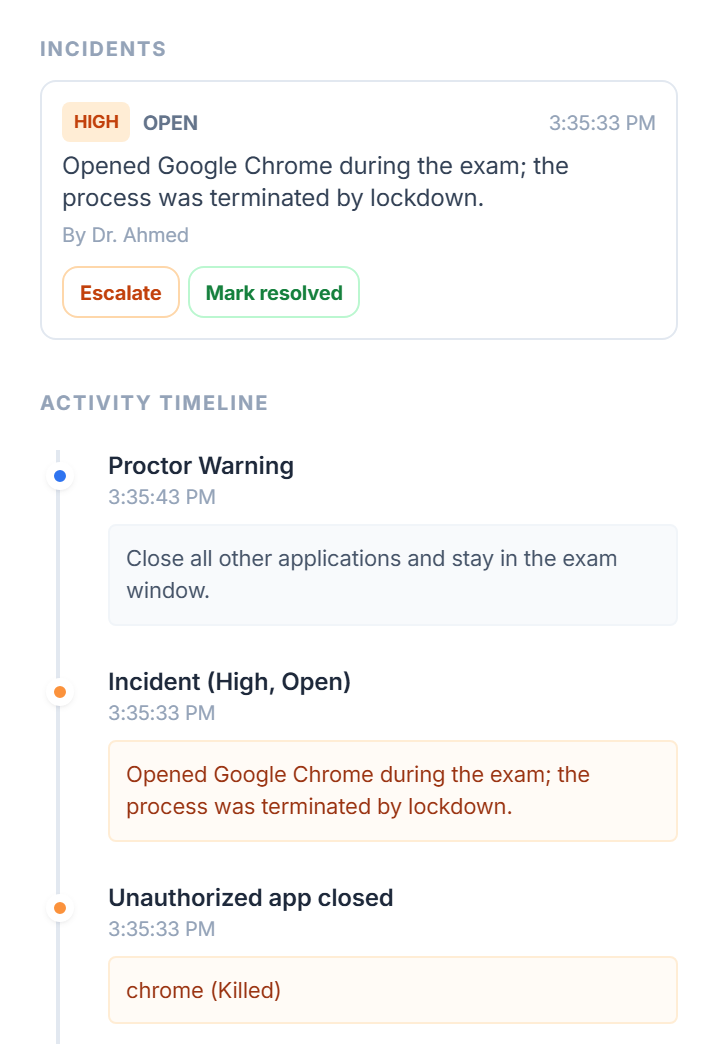
\includegraphics[width=0.60\linewidth,height=418pt,keepaspectratio]{Figures/ui_live_timeline.png}
\caption{Student Drawer (c): Incident and Activity Timeline}
\label{fig:ui_live_timeline}
\end{figure}
\SoftBarrierN

\subsection{Evaluation}\suppressfloats[t]
The results page lists each submission with its score and SHA-256 receipt. Opening one (Figures~\ref{fig:ui_teacher_ai_grading} and~\ref{fig:ui_teacher_ai_grading_b}) shows every answer next to its AI evaluation: suggested mark, confidence, engine, justification, test-case results (hidden cases marked) and code-analysis signals. Coding answers (C or C++ only) are compiled and run against weighted test cases \cite{alamutka2005} in an isolated Docker \texttt{gcc:13} container when Docker is available; otherwise a local MinGW g++ runner, which is not isolated, is used, and with no runner the answer is left for teacher review (FR11.1). Theory answers get a TF-IDF similarity score \cite{salton1988} (FR11.2). The teacher accepts the mark or saves an override, stored in \texttt{TeacherGradeOverrides}.

Figure~\ref{fig:ui_teacher_ai_grading} shows the top of the review for Usman Tariq: his status (Submitted), the question with its type and maximum (Coding, 20 marks) and his submitted code. His program starts the maximum at 0 instead of at the first element, so it prints a wrong answer when all the numbers are negative. The evaluation card below shows how the grader finds this mistake.

\begin{figure}[tbp]
\centering
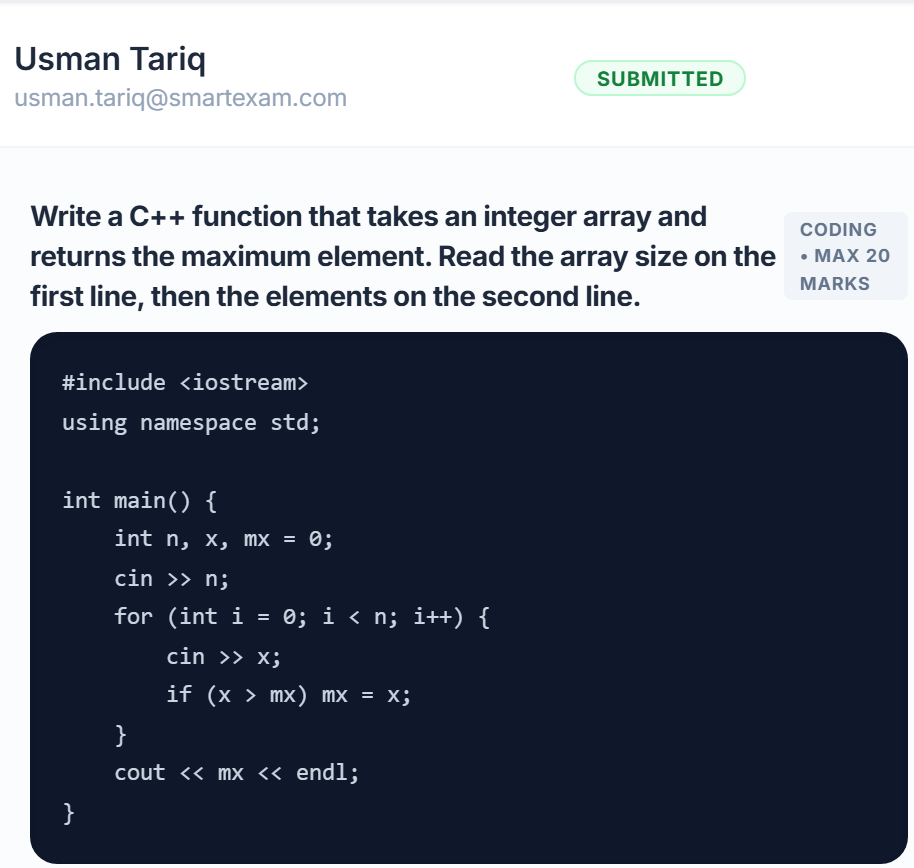
\includegraphics[width=0.85\linewidth,height=370pt,keepaspectratio]{Figures/ui_ai_grading_answer.png}
\caption{AI Evaluation of a Coding Answer (a): Question and Submitted Code}
\label{fig:ui_teacher_ai_grading}
\end{figure}
\SoftBarrierN

The AI evaluation card (Figure~\ref{fig:ui_teacher_ai_grading_b}) suggests 10 of 20 marks with medium confidence, from the isolated Docker engine. The test-case table explains the mark: the visible case passes, but the hidden case with the input $-1$, $-5$, $-2$ expects $-1$ and gets 0, so one of the two cases passes and half the marks are suggested. The code-analysis signals give O($n$) complexity, one loop and a medium hard-coding suspicion, because the code passes every visible case but fails a hidden one. The teacher can accept the 10 marks or enter another mark with a note and click \emph{Save Grade Override}.

\begin{figure}[tbp]
\centering
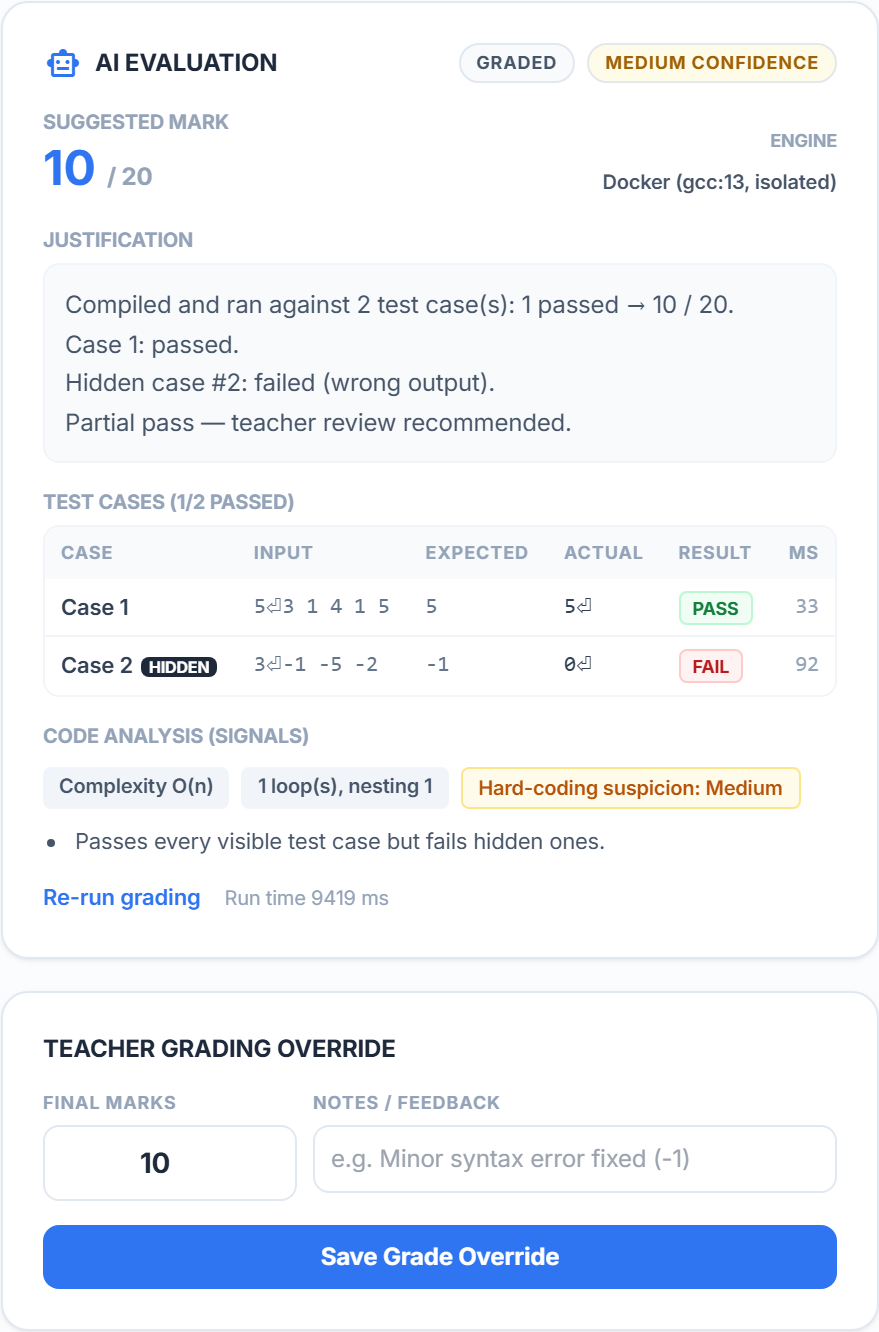
\includegraphics[width=\linewidth,height=565pt,keepaspectratio]{Figures/ui_ai_grading_eval.png}
\caption{AI Evaluation of a Coding Answer (b): Suggested Mark, Test Cases and Override}
\label{fig:ui_teacher_ai_grading_b}
\end{figure}
\SoftBarrierN

The \emph{Plagiarism Flags} tab (Figure~\ref{fig:ui_plagiarism}) shows a pairwise heat map built by k-gram winnowing \cite{winnowing}, which ignores identifiers and comments in code (FR11.3). A pair at or above the exam's threshold gets a card with both answers side by side and the matched lines highlighted; here Sara's program is Ali's with renamed variables. The teacher records the decision as a grade override.

In the heat map each row and column is a student (the columns use initials), and each cell is the highest similarity of that pair over all questions; darker cells are more similar, in 20\,\% steps. Only Ali Hassan and Sara Khan reach the 70\,\% threshold, at 100\,\%, while every other pair is at 25\,\% or below. The card below shows why: only the names differ (\texttt{largest}, \texttt{nums}, \texttt{top} against \texttt{findMax}, \texttt{arr}, \texttt{best}), so with identifiers ignored the code is the same. A note at the bottom reminds the teacher that similarity is evidence, not a verdict.

\begin{figure}[p]
\centering
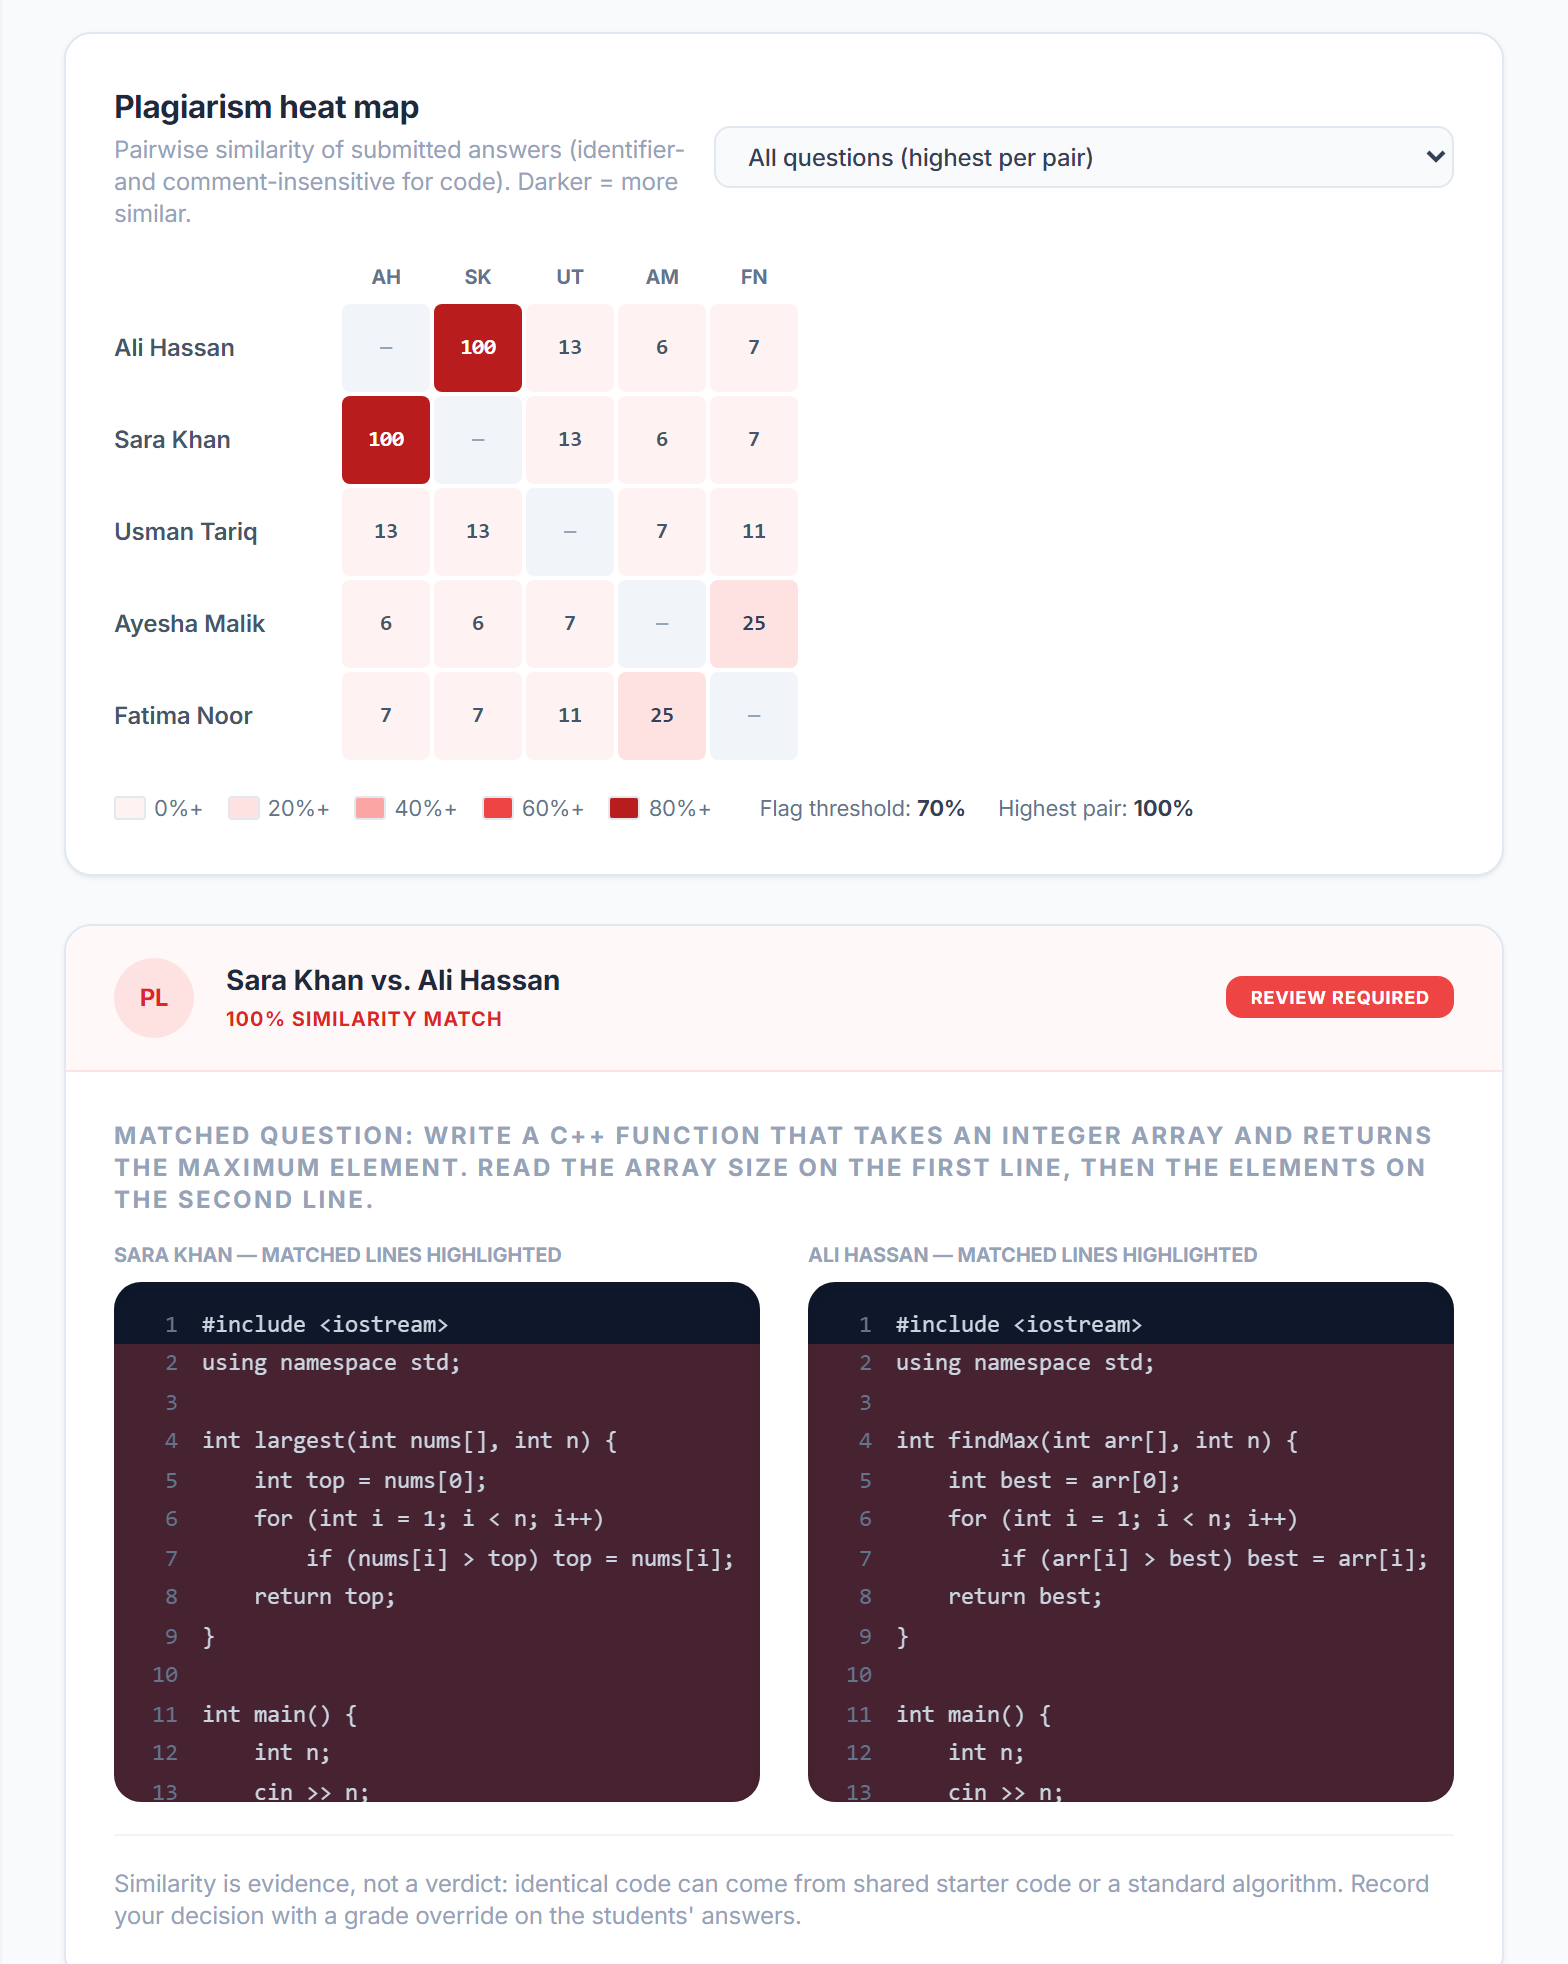
\includegraphics[width=\linewidth,height=562pt,keepaspectratio]{Figures/ui_plagiarism.png}
\caption{Plagiarism Heat Map and Matched Pair}
\label{fig:ui_plagiarism}
\end{figure}
\SoftBarrierN

\subsection{Administration and Student Portal}\suppressfloats[t]
Every web user, staff or student, signs in on one login page with email and password (Figure~\ref{fig:ui_web_login}) and is taken to the home page of their role. Neither front end offers self-registration or an emailed password reset: administrators create accounts or import them from a CSV file and can set a new password when editing an account (FR7), and staff change their own password from the panel (Figure~\ref{fig:seq_change_password}). The desktop client's sign-in and logout are drawn in Figures~\ref{fig:seq_login} and~\ref{fig:seq_logout}; on the web panel, sign-in, refresh and sign-out are tested in ST-01 (Table~\ref{tab:st_admin}). The figure shows the form filled in for the teacher account (\texttt{teacher@smartexam.com}), with an eye icon to show or hide the password. The note under \emph{Sign In} says that access attempts are logged, and this is true: the server writes every successful and failed login to the audit log (\texttt{LOGIN\_SUCCESS}, \texttt{LOGIN\_FAILED}).

\begin{figure}[htbp]
\centering
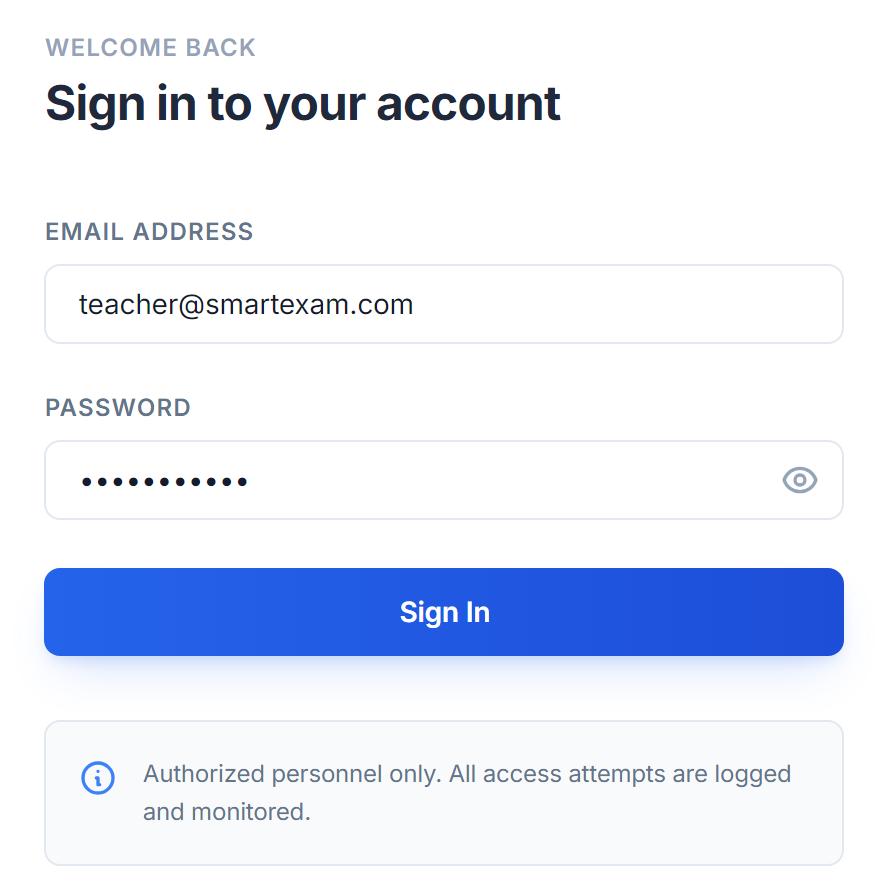
\includegraphics[width=0.62\linewidth]{Figures/ui_web_login.png}
\caption{Web Panel Login (Sign-In Form)}
\label{fig:ui_web_login}
\end{figure}
\SoftBarrierN

Admins manage departments and courses (Figure~\ref{fig:ui_academics}); department names are unique, a course code is unique within its department, and a department or course still in use cannot be deleted (FR7). The upper card lists the three departments with their number of courses (Computer Science 3, Electrical Engineering 1, Software Engineering 2). The lower card lists the six courses with code, name, department and number of sections, and can be filtered by department. Only CS301 Data Structures has a section, the one that owns the demo exams, so it is the only course here that cannot be deleted.

\begin{figure}[tbp]
\centering
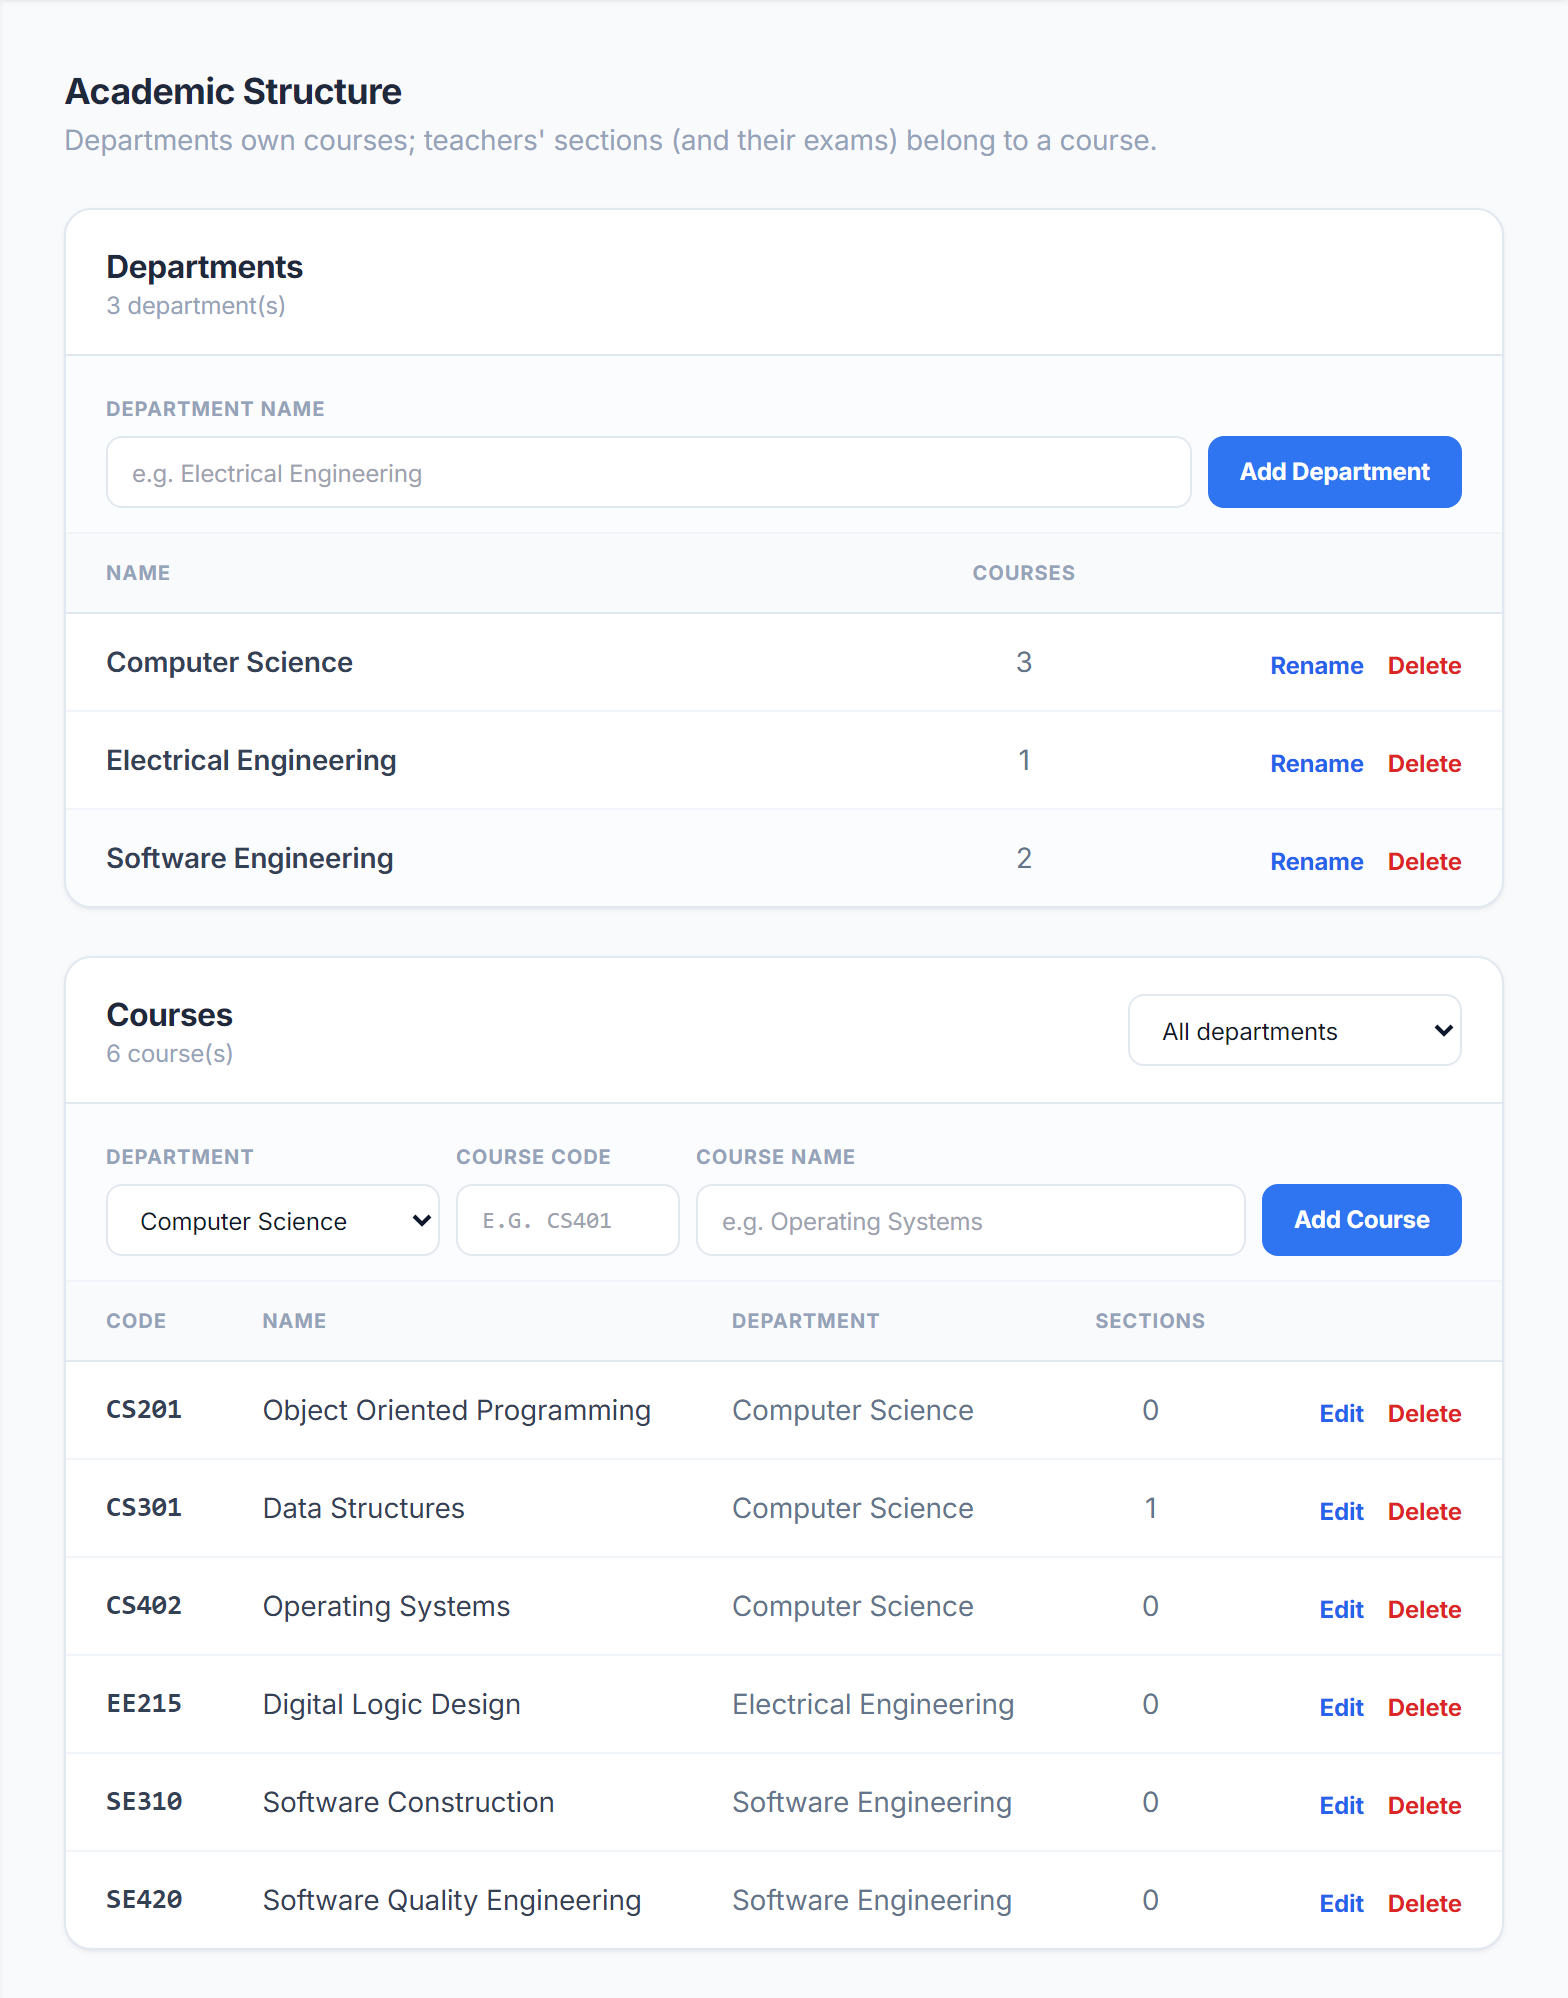
\includegraphics[width=\linewidth,height=600pt,keepaspectratio]{Figures/ui_academics.png}
\caption{Departments and Courses}
\label{fig:ui_academics}
\end{figure}
\SoftBarrierN

Admins register labs and workstations (machine number, Windows PC name, IP address) in Figure~\ref{fig:ui_labs_workstations}; each seat shows the student signed in on it. With \texttt{EnforceSeat} on, a student with a seat can start the exam only from that PC (FR9). The figure shows Lab~A (Demo) in Block~3, Ground Floor, with six workstations; each card gives the seat name, the IP address and the PC name. A green \emph{In use} card also shows the signed-in student, the Windows user and when the PC was last seen. R2C2 is \emph{Free} because Hamza Iqbal, who is seated there, is not eligible and has not signed in.

\begin{figure}[tbp]
\centering
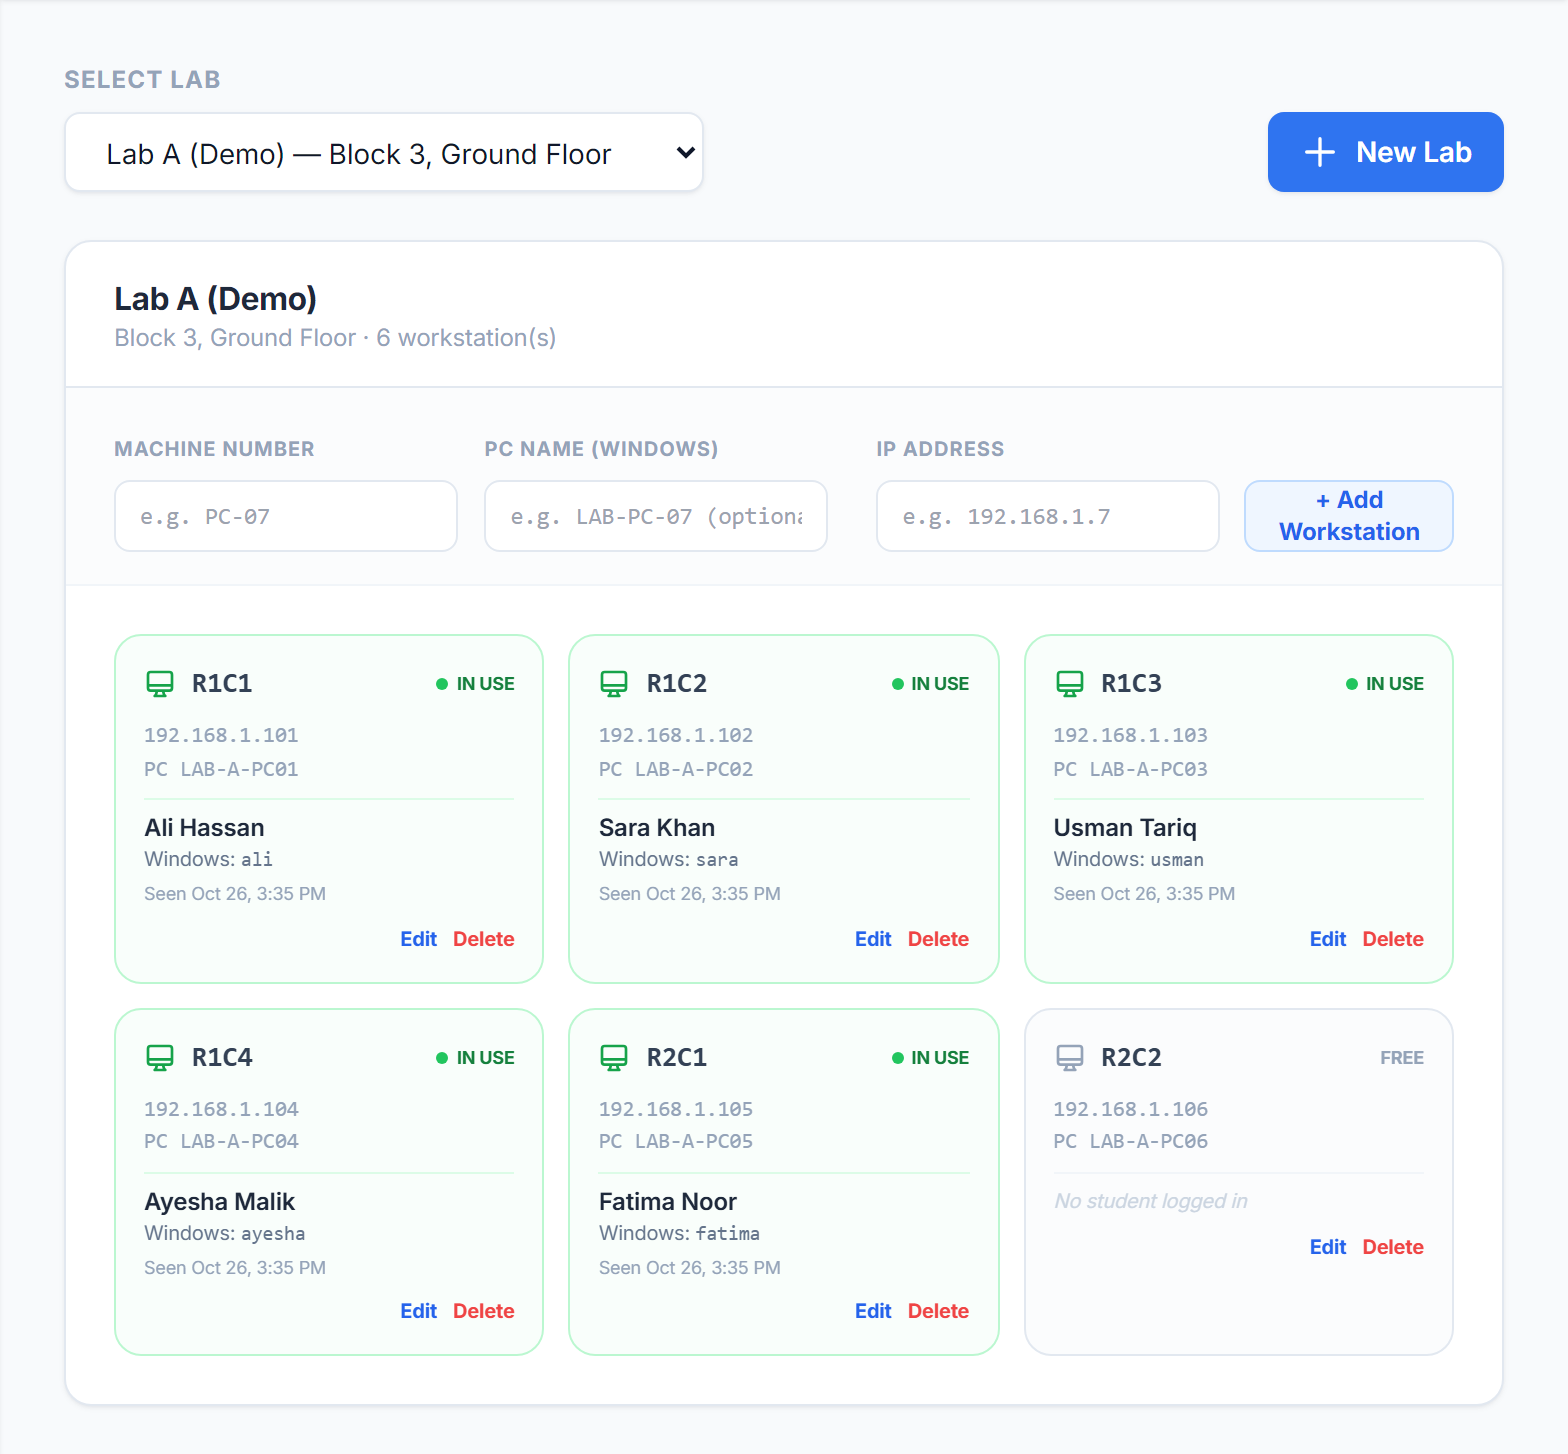
\includegraphics[width=\linewidth,height=418pt,keepaspectratio]{Figures/ui_labs_workstations.png}
\caption{Labs and Workstations}
\label{fig:ui_labs_workstations}
\end{figure}
\SoftBarrierN

The device-binding page (Figure~\ref{fig:ui_device_bindings}) lists each student's binding status, bound PC and last-seen time (FR1). \emph{Reset Binding} (\texttt{DELETE /api/users/\{id\}/device-binding}) removes the binding and revokes all the student's tokens, so the next login binds a new PC; \emph{Force Logout} only revokes the tokens. In the figure the five students who have signed in are \emph{Bound} to LAB-A-PC01 to LAB-A-PC05, while Hamza Iqbal is \emph{Unbound}, so his row has no PC and no actions. A search box and a \emph{Show unbound only} switch help the administrator find a student, and the note at the top says that an administrator can reset a binding after a genuine hardware change or a login problem.

\begin{figure}[tbp]
\centering
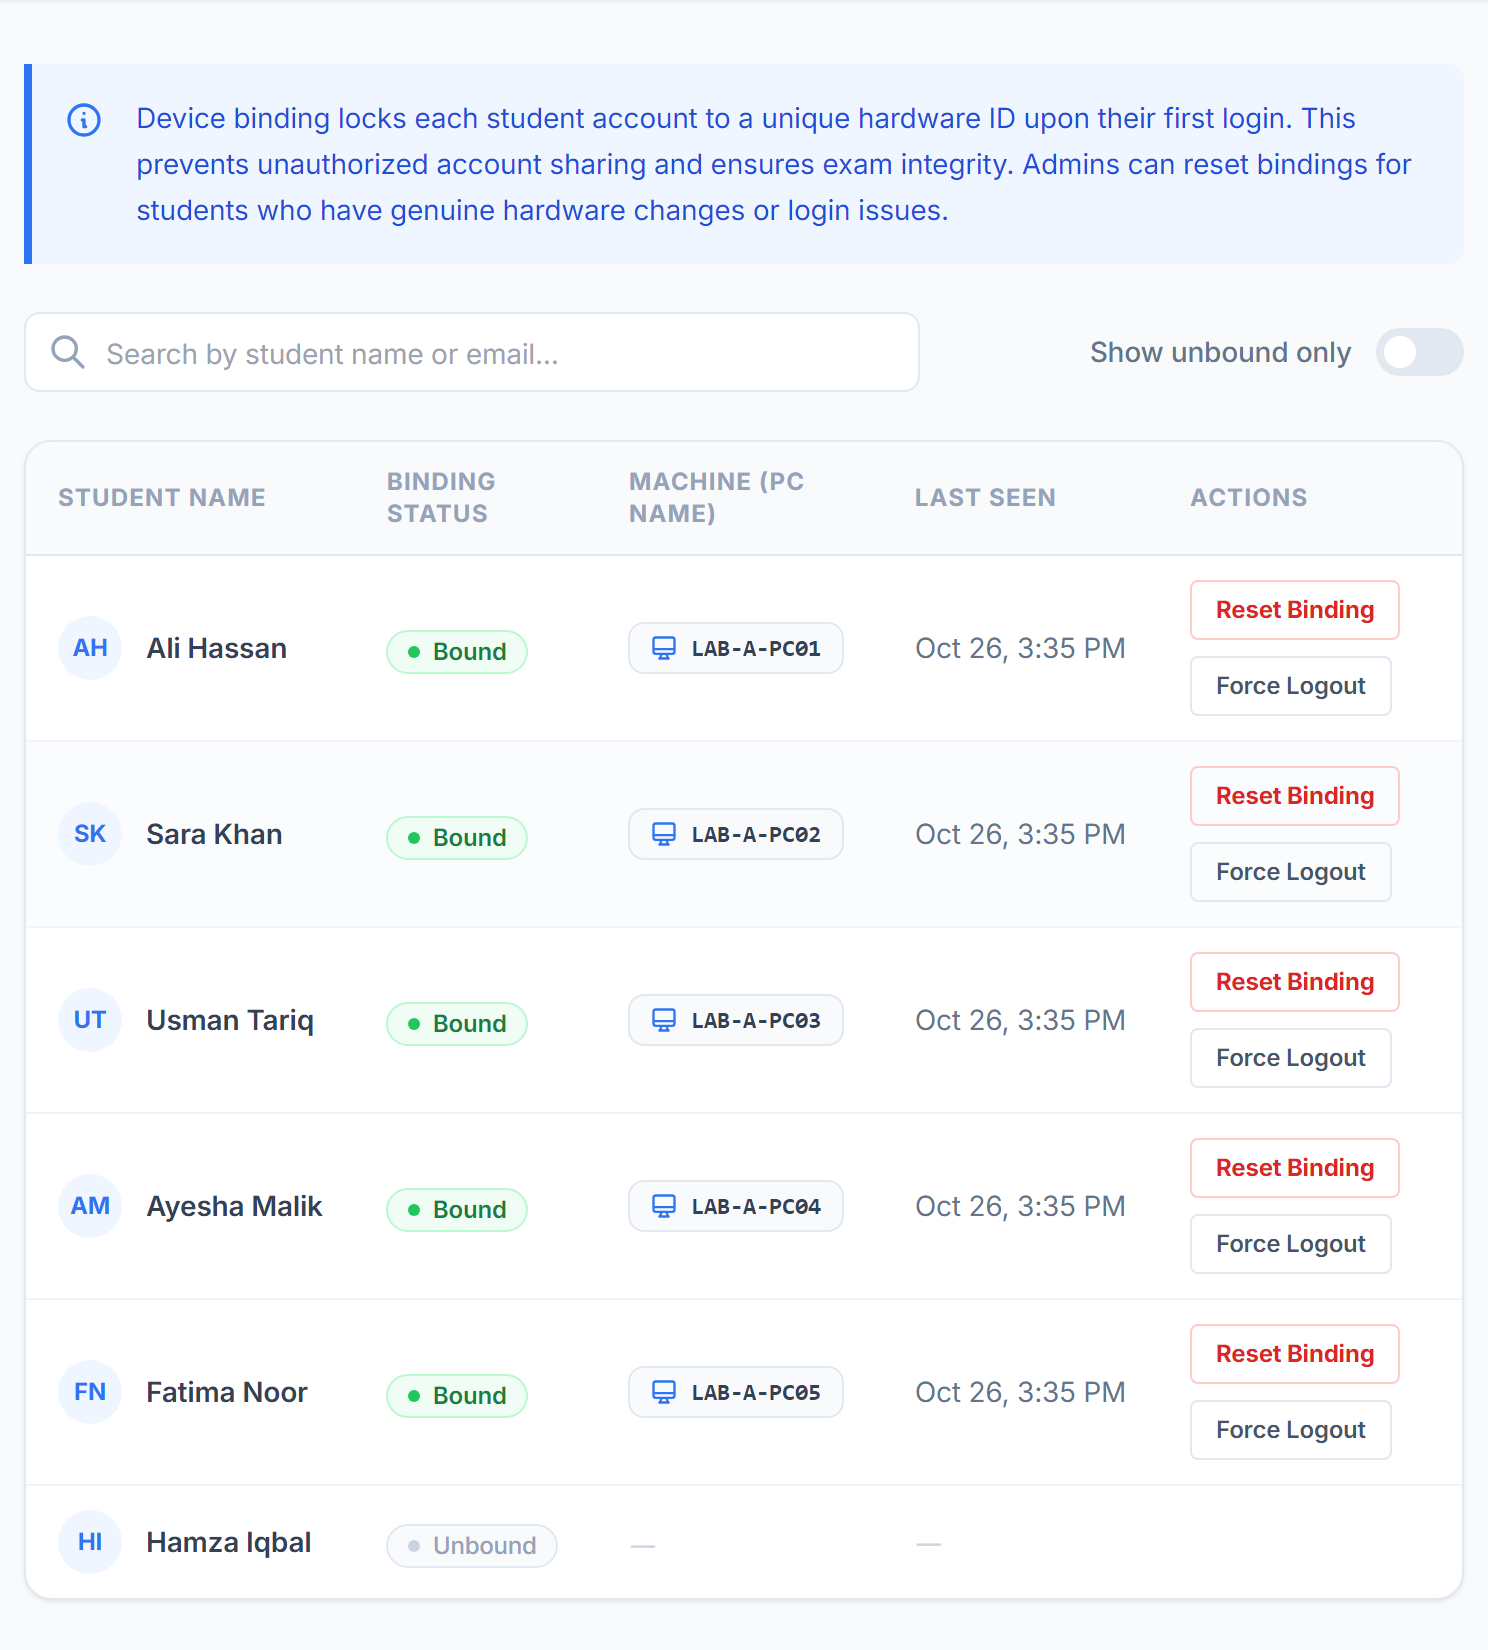
\includegraphics[width=\linewidth,height=500pt,keepaspectratio]{Figures/ui_device_bindings.png}
\caption{Device Bindings (Email, Windows User and Registered Columns Omitted)}
\label{fig:ui_device_bindings}
\end{figure}
\SoftBarrierN

The read-only audit page (Figure~\ref{fig:ui_audit_logs}) lists \texttt{AuditLogs} rows (time, actor, event, entity, JSON details) for security-relevant and staff actions, such as logins, grade overrides, completed AI grading and submissions (FR12). The newest rows come first, and the actor is a user with an email or \emph{System} for background jobs. The visible rows follow the end of the demo exam, from the warning sent to Usman (\texttt{PROCTOR\_WARNING\_SENT}, 3:35:43~PM) through three submissions (\texttt{SESSION\_SUBMITTED}) and the background grading (\texttt{AI\_GRADING\_COMPLETED}) to a grade override by Dr. Ahmed and a new login by Ali Hassan. The green badge \emph{Chain verified (91 entries)} at the top shows that the hash chain over these rows verifies, and \emph{Re-verify} runs the check again.

\begin{figure}[tbp]
\centering
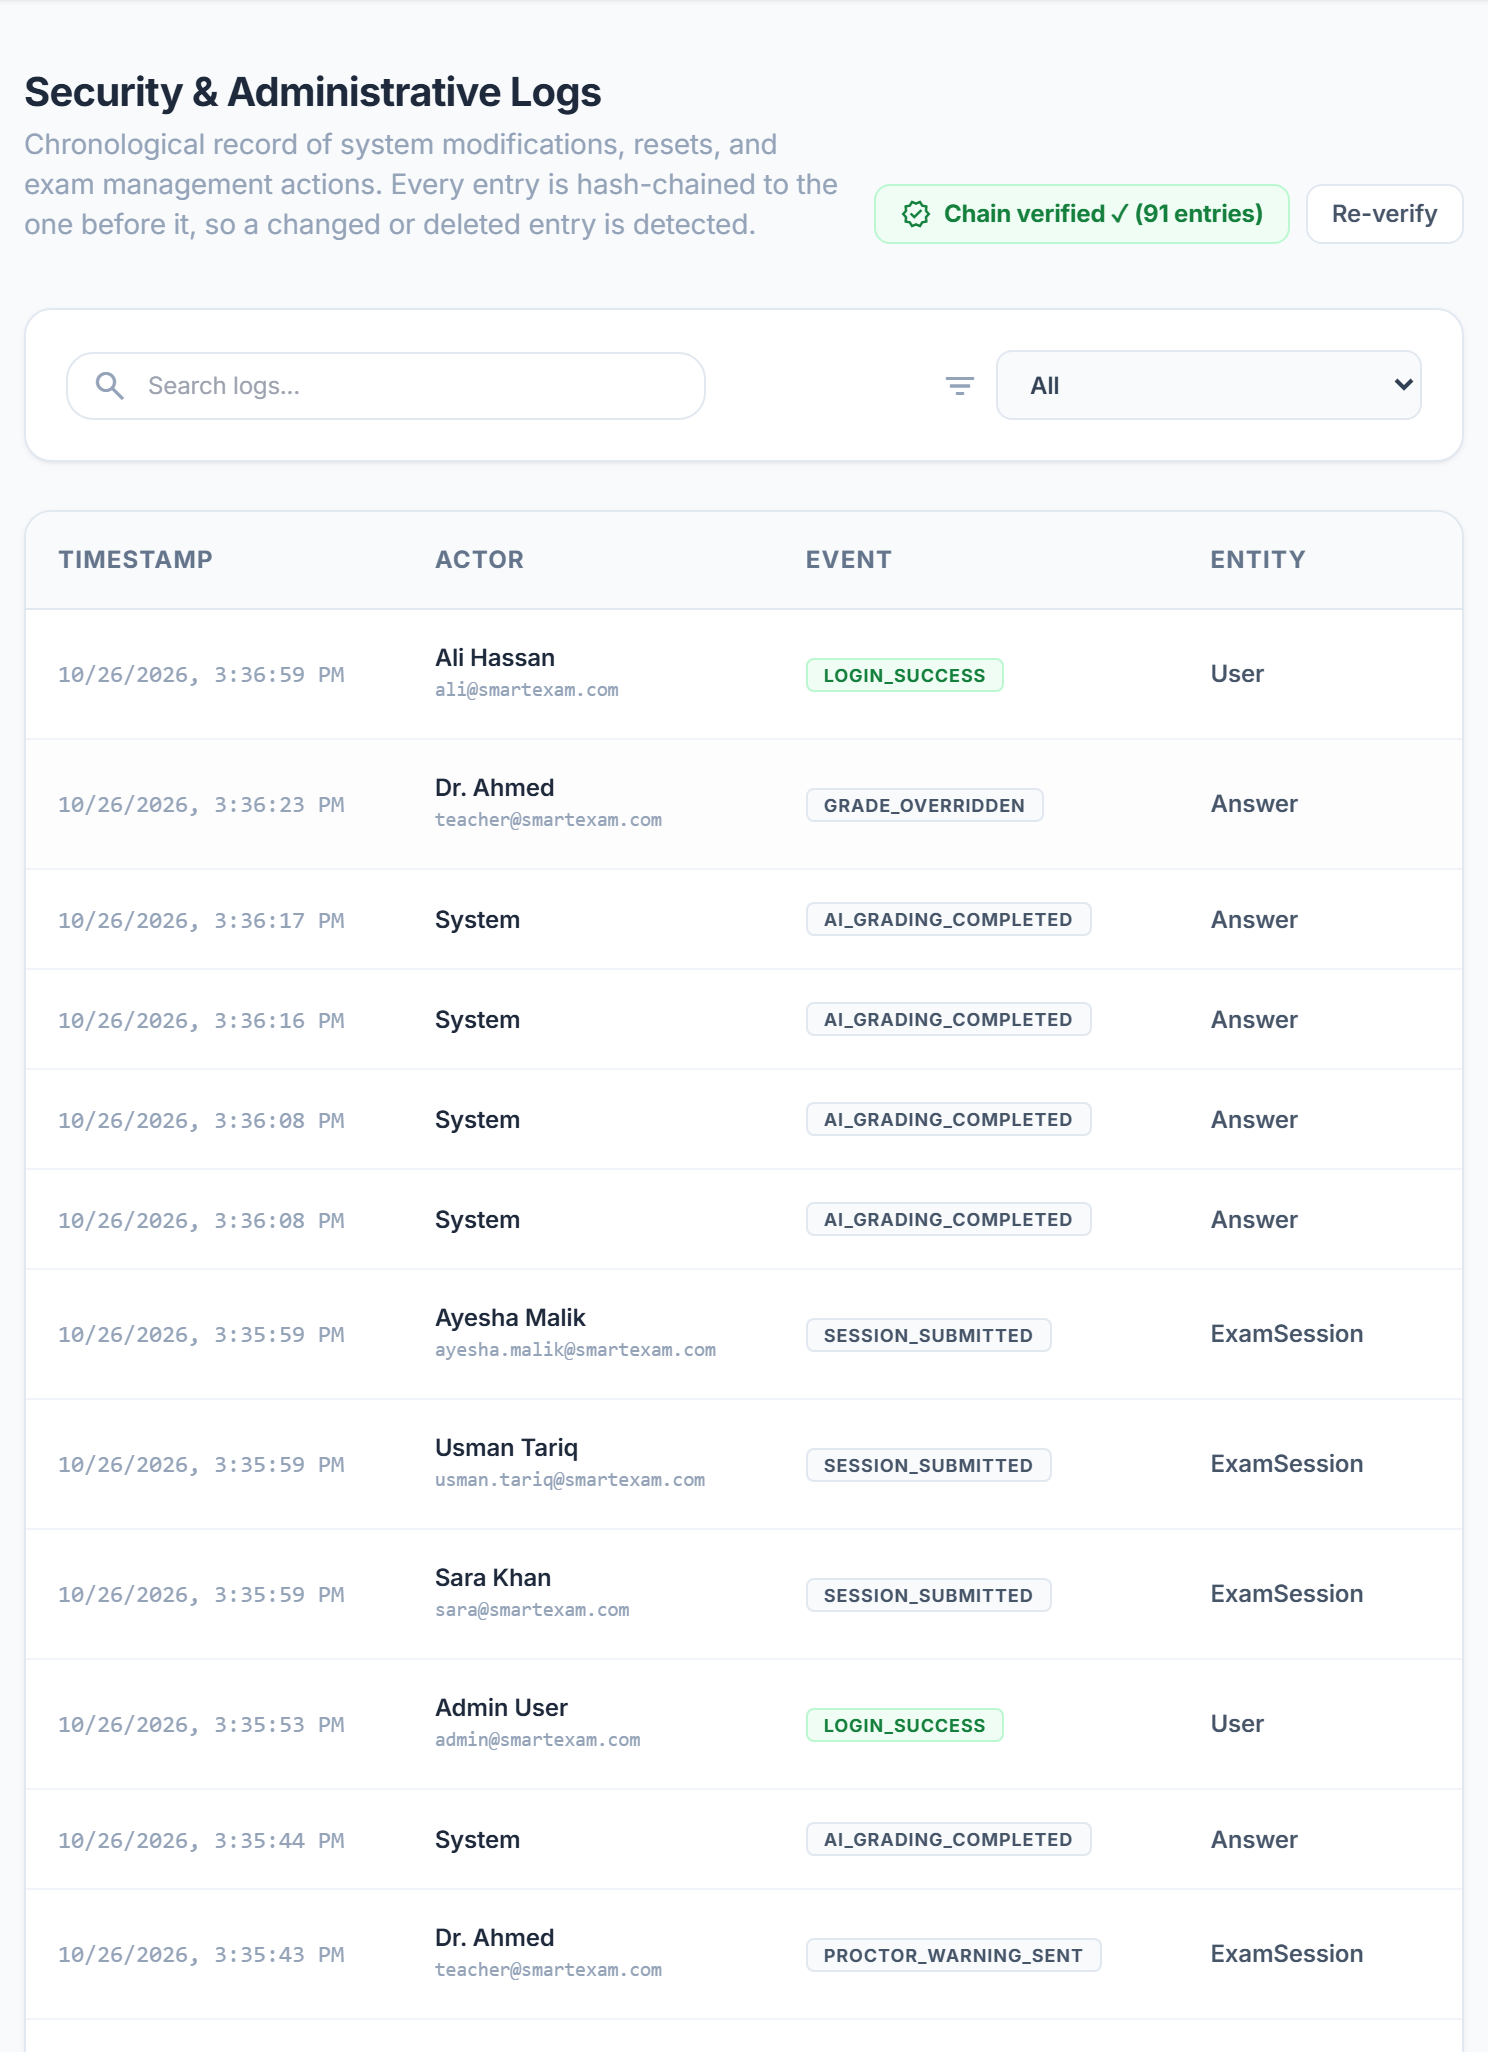
\includegraphics[width=\linewidth,height=622pt,keepaspectratio]{Figures/ui_audit_logs.png}
\caption{Audit Log Page (Details Column Omitted)}
\label{fig:ui_audit_logs}
\end{figure}
\SoftBarrierN

In the student portal (Figures~\ref{fig:ui_student_performance} to~\ref{fig:ui_student_performance_b}) a student sees exams taken, average and best score, integrity flags, a score trend, the score of each exam and an exam timeline; practice exams do not count towards results (they are auto-marked but never plagiarism-checked and are hidden from the student's results). The summary cards (Figure~\ref{fig:ui_student_performance}) show four exams taken, an average of 85.9\,\%, a best score of 93.3\,\% and no flags; the flag count adds up the violations recorded in the student's sessions. The average matches the mean of the four scores in the timeline (80, 83.3, 93.3 and 87.1\,\%).

\begin{figure}[tbp]
\centering
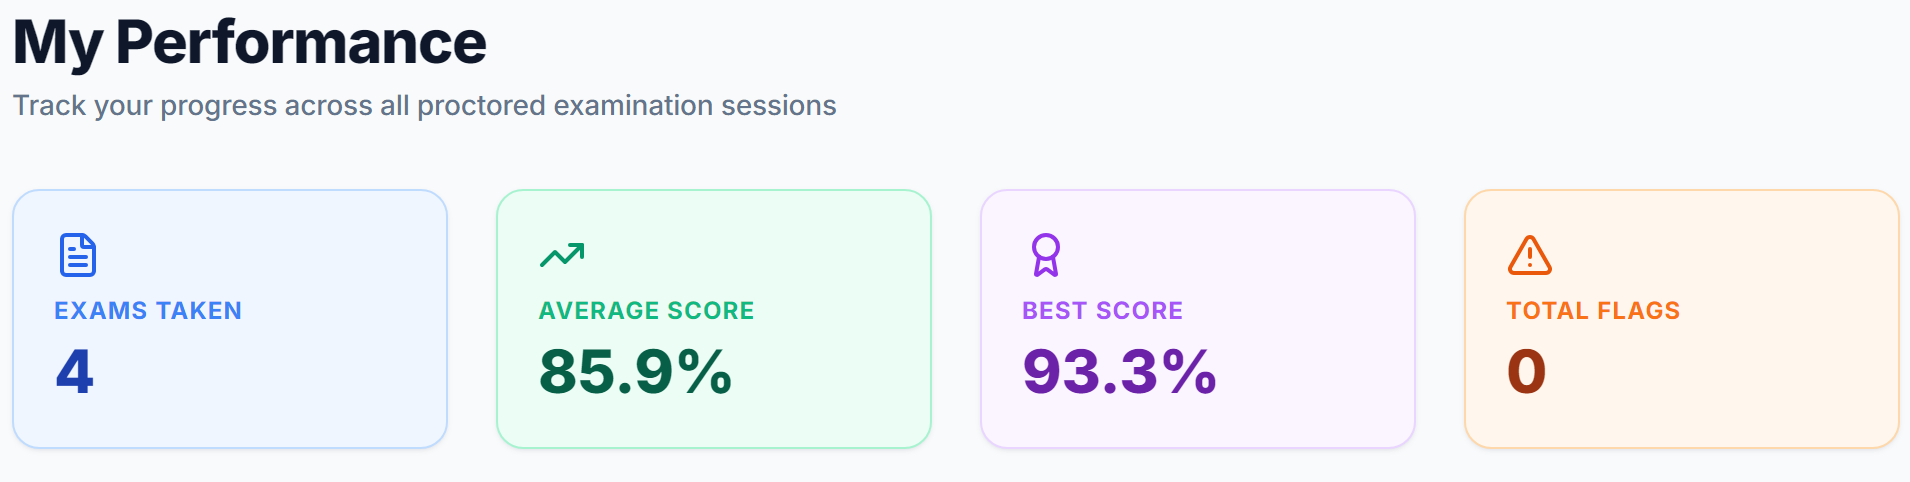
\includegraphics[width=\linewidth]{Figures/ui_student_performance_a_p1.png}
\caption{Student Performance Page (a): Summary Cards}
\label{fig:ui_student_performance}
\end{figure}
\SoftBarrierN

The \emph{Score Over Time} chart (Figure~\ref{fig:ui_student_performance_trend}) draws the same scores in date order, from Lab Exam~1 to the Mid-Term Lab Exam, above a dashed pass-mark line at 50\,\%. The \emph{Improving trend} badge appears because the latest score is higher than the first one. Figure~\ref{fig:ui_student_performance_b} shows the four exams again as bars, with the score rounded to a whole percent, and as a timeline, newest first, with the date and exact score of each exam.

\begin{figure}[tbp]
\centering
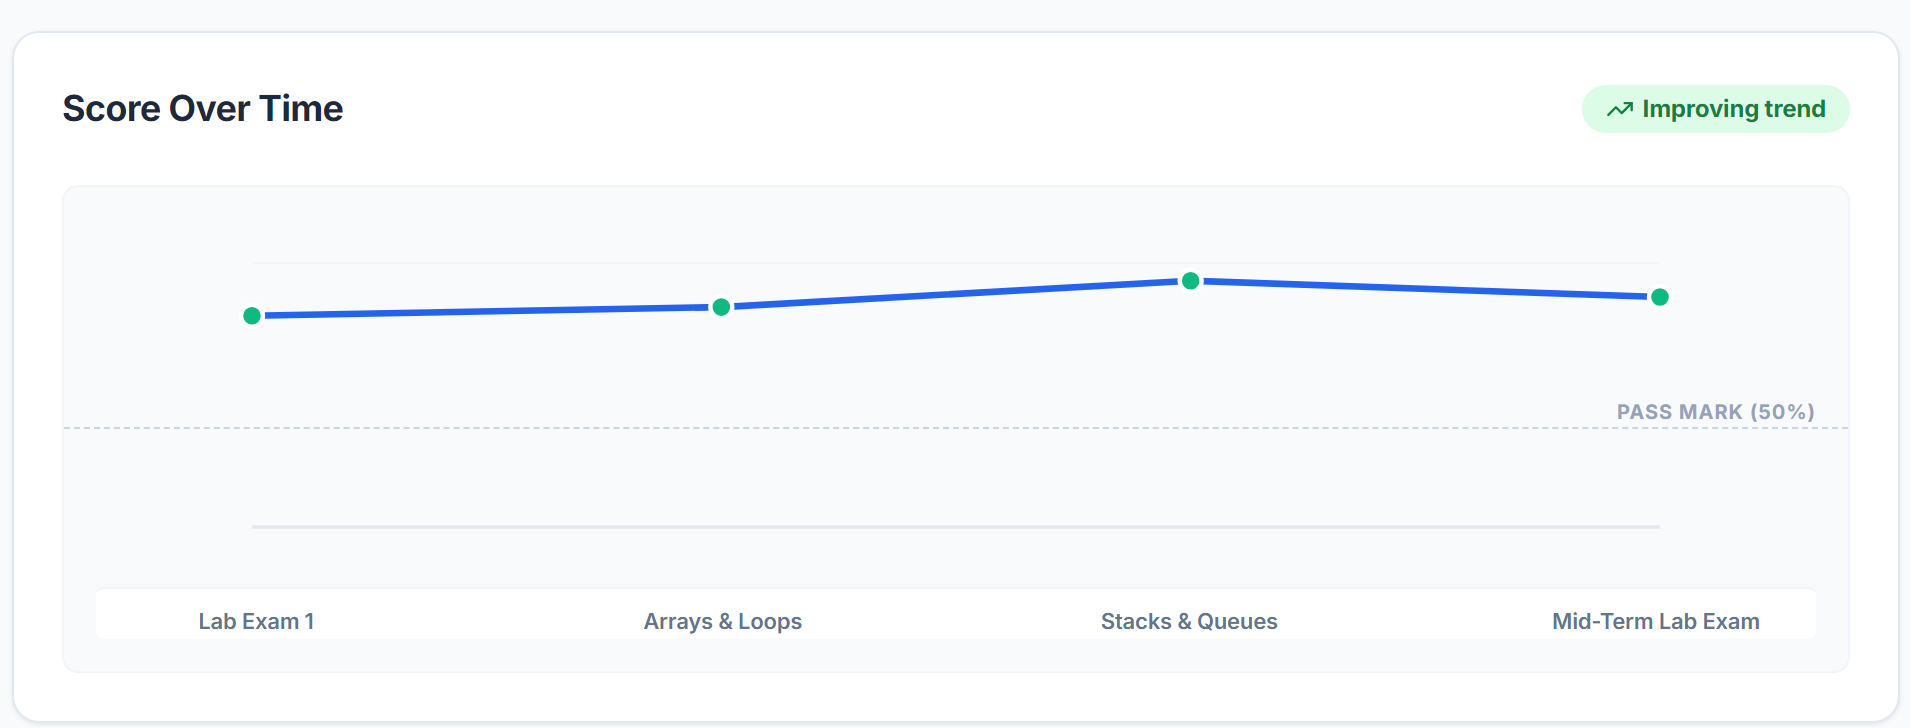
\includegraphics[width=\linewidth]{Figures/ui_student_performance_a_p2.png}
\caption{Student Performance Page (b): Score Trend}
\label{fig:ui_student_performance_trend}
\end{figure}
\SoftBarrierN

\begin{figure}[tbp]
\centering
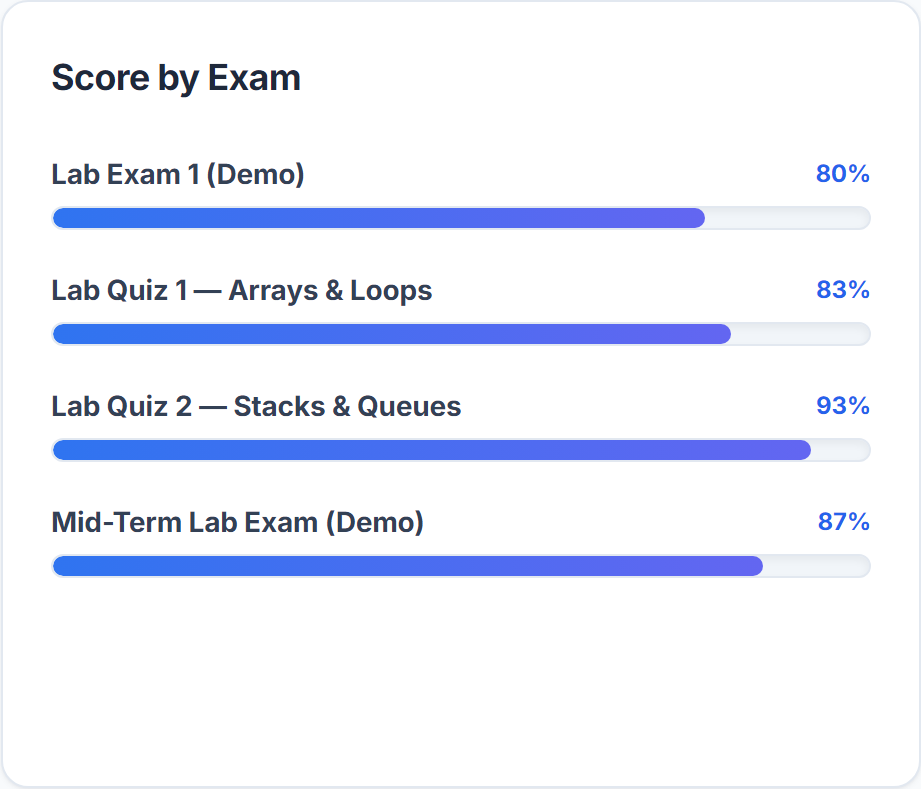
\includegraphics[width=0.7\linewidth]{Figures/ui_student_performance_scores.png}\\[4pt]
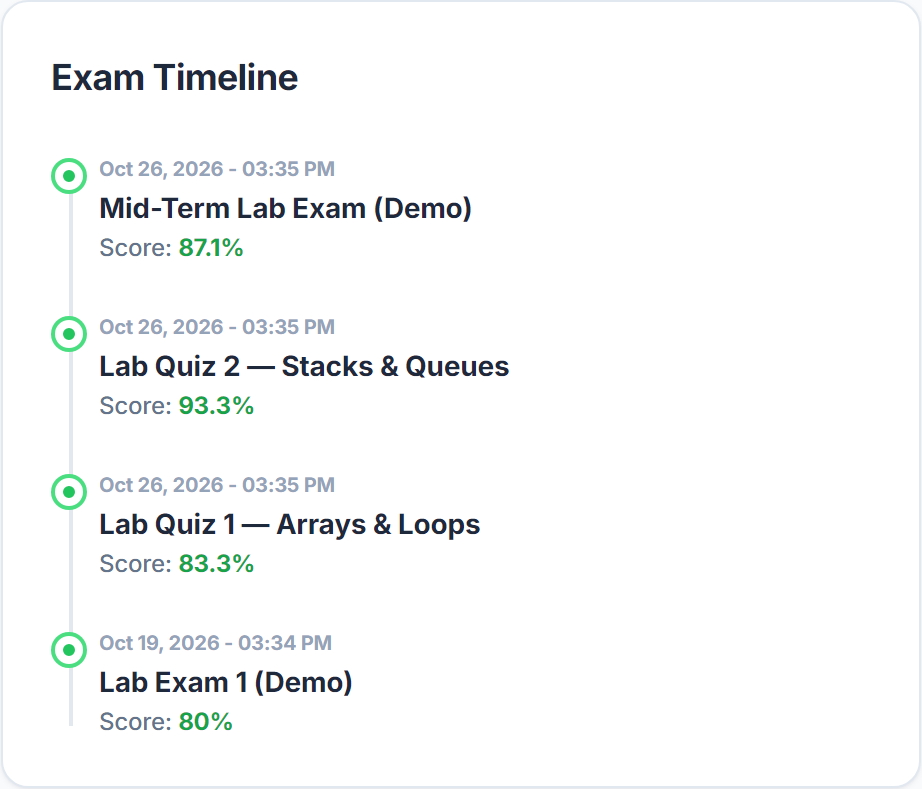
\includegraphics[width=0.7\linewidth]{Figures/ui_student_performance_timeline.png}
\caption{Student Performance Page (c): Score by Exam and Exam Timeline Cards}
\label{fig:ui_student_performance_b}
\end{figure}
\SoftBarrierN

\clearpage
\renewcommand{\topfraction}{0.7}\renewcommand{\bottomfraction}{0.3}
\renewcommand{\textfraction}{0.2}\renewcommand{\floatpagefraction}{0.5}
\section{Physical Database Tables}
\label{sec:physical_tables}
% Database tables, one per entity of the ERD (Figures erd_diagram and erd_diagram_b), in ERD order.
% Columns, types, keys and lengths follow Backend_API/Data/AppDbContext.cs and the EF Core model snapshot.

\label{sec:db_tables_detail}
This section gives one table for each entity of the ERD (Figures~\ref{fig:erd_diagram} and~\ref{fig:erd_diagram_b}), in the same order as the diagram, 29 tables in all. Each table lists every column that EF Core creates in PostgreSQL, with its data type, its key or constraint and a short description. In the tables, PK means primary key, FK means foreign key (the table it points to is in brackets), \texttt{uuid} is a globally unique identifier and \texttt{timestamptz} is a timestamp with time zone; key columns are never null, and a column marked ``no FK'' holds an id without a foreign-key constraint.

\par\ifdim\dimexpr\pagegoal-\pagetotal\relax<362pt\newpage\fi
\subsection{Users Table}
The \texttt{Users} table stores every account in the system, for all five roles: SuperAdmin, Admin, Teacher, Invigilator and Student. Most other tables point to it, for example \texttt{DeviceBindings}, \texttt{Sections} for the teacher and \texttt{ExamSessions} for the student. \texttt{Email} is unique, and \texttt{RollNumber} is unique whenever it is set.

{\small
\begin{longtable}{>{\raggedright\arraybackslash}p{3.4cm}>{\raggedright\arraybackslash}p{2.6cm}>{\raggedright\arraybackslash}p{2.6cm}>{\raggedright\arraybackslash}p{5.6cm}}
\caption{Users Table}\label{tab:db_users}\\
\hline\hline
\textbf{Field Name} & \textbf{Data Type} & \textbf{Key / Constraint} & \textbf{Description} \\ \hline
\endfirsthead
\multicolumn{4}{c}{\tablename~\thetable{} -- continued from previous page}\\
\hline\hline
\textbf{Field Name} & \textbf{Data Type} & \textbf{Key / Constraint} & \textbf{Description} \\ \hline
\endhead
\hline \multicolumn{4}{r}{Continued on next page}\\
\endfoot
\hline\hline
\endlastfoot
UserId & uuid & PK & Unique id of the user \\*
Name & text & Not null & Display name \\*
Email & text & Not null, unique & Email address, used to log in \\
RollNumber & varchar(32) & Null, unique when set & University roll number, stored in upper case; students may log in with it \\
PasswordHash & text & Not null & Salted PBKDF2 hash of the password \\
Salt & text & Not null & Random salt used for the hash \\*
Role & text & Not null & SuperAdmin, Admin, Teacher, Invigilator or Student \\*
IsActive & boolean & Not null & False when the account is deactivated; default true \\*
CreatedAt & timestamptz & Not null & When the account was created \\
\end{longtable}
}

\par\ifdim\dimexpr\pagegoal-\pagetotal\relax<362pt\newpage\fi
\subsection{DeviceBindings Table}
The \texttt{DeviceBindings} table links a user to the one PC the account is bound to. \texttt{UserId} is a foreign key to \texttt{Users} and is also unique, so a user has at most one binding, and the binding is deleted together with the user.

{\small
\begin{longtable}{>{\raggedright\arraybackslash}p{3.4cm}>{\raggedright\arraybackslash}p{2.6cm}>{\raggedright\arraybackslash}p{2.6cm}>{\raggedright\arraybackslash}p{5.6cm}}
\caption{DeviceBindings Table}\label{tab:db_devicebindings}\\
\hline\hline
\textbf{Field Name} & \textbf{Data Type} & \textbf{Key / Constraint} & \textbf{Description} \\ \hline
\endfirsthead
\multicolumn{4}{c}{\tablename~\thetable{} -- continued from previous page}\\
\hline\hline
\textbf{Field Name} & \textbf{Data Type} & \textbf{Key / Constraint} & \textbf{Description} \\ \hline
\endhead
\hline \multicolumn{4}{r}{Continued on next page}\\
\endfoot
\hline\hline
\endlastfoot
BindingId & uuid & PK & Unique id of the binding \\*
UserId & uuid & FK (Users), unique & The bound user \\*
HwidHash & text & Not null & SHA-256 hash of the PC's hardware fingerprint \\
HwidVersion & integer & Not null & Fingerprint format: 1 = old, 2 = current; default 1 \\
MachineName & text & Null & Windows computer name, e.g. LAB-PC-07 \\*
WindowsUsername & text & Null & Windows account logged in on that PC \\*
RegisteredAt & timestamptz & Not null & When the PC was bound \\*
LastSeenAt & timestamptz & Not null & Last time the bound PC was seen \\
\end{longtable}
}

\par\ifdim\dimexpr\pagegoal-\pagetotal\relax<314pt\newpage\fi
\subsection{UserSessions Table}
The \texttt{UserSessions} table keeps one row for each access token issued at login, stored by its JWT ID, so that a token can be revoked before it expires. A user can have many rows, and the rows are deleted with the user. \texttt{Jti} is unique.

{\small
\begin{longtable}{>{\raggedright\arraybackslash}p{3.4cm}>{\raggedright\arraybackslash}p{2.6cm}>{\raggedright\arraybackslash}p{2.6cm}>{\raggedright\arraybackslash}p{5.6cm}}
\caption{UserSessions Table}\label{tab:db_usersessions}\\
\hline\hline
\textbf{Field Name} & \textbf{Data Type} & \textbf{Key / Constraint} & \textbf{Description} \\ \hline
\endfirsthead
\multicolumn{4}{c}{\tablename~\thetable{} -- continued from previous page}\\
\hline\hline
\textbf{Field Name} & \textbf{Data Type} & \textbf{Key / Constraint} & \textbf{Description} \\ \hline
\endhead
\hline \multicolumn{4}{r}{Continued on next page}\\
\endfoot
\hline\hline
\endlastfoot
SessionId & uuid & PK & Unique id of the row \\*
UserId & uuid & FK (Users) & Owner of the token \\*
Jti & text & Not null, unique & JWT ID of the access token \\*
ExpiresAt & timestamptz & Not null & When the token expires \\*
IsRevoked & boolean & Not null & True once the token is revoked; default false \\*
CreatedAt & timestamptz & Not null & When the token was issued \\
\end{longtable}
}

\par\ifdim\dimexpr\pagegoal-\pagetotal\relax<362pt\newpage\fi
\subsection{RefreshTokens Table}
The \texttt{RefreshTokens} table stores the rotating refresh tokens; only the SHA-256 hash of each token is kept, never the token itself. Every login starts a new token family, and each refresh revokes the used token and issues the next one in the same family. Each row belongs to one user and is deleted with that user; \texttt{TokenHash} is unique.

{\small
\begin{longtable}{>{\raggedright\arraybackslash}p{3.4cm}>{\raggedright\arraybackslash}p{2.6cm}>{\raggedright\arraybackslash}p{2.6cm}>{\raggedright\arraybackslash}p{5.6cm}}
\caption{RefreshTokens Table}\label{tab:db_refreshtokens}\\
\hline\hline
\textbf{Field Name} & \textbf{Data Type} & \textbf{Key / Constraint} & \textbf{Description} \\ \hline
\endfirsthead
\multicolumn{4}{c}{\tablename~\thetable{} -- continued from previous page}\\
\hline\hline
\textbf{Field Name} & \textbf{Data Type} & \textbf{Key / Constraint} & \textbf{Description} \\ \hline
\endhead
\hline \multicolumn{4}{r}{Continued on next page}\\
\endfoot
\hline\hline
\endlastfoot
TokenId & uuid & PK & Unique id of the token \\*
UserId & uuid & FK (Users) & Owner of the token \\*
FamilyId & uuid & Not null, indexed & Token family started at login \\
TokenHash & varchar(64) & Not null, unique & SHA-256 hash of the raw token \\
Jti & varchar(64) & Not null, indexed & JWT ID of the access token issued with it \\
Channel & varchar(32) & Not null & web or student-client \\
MachineName & varchar(128) & Null & PC name, sent again as the machine claim on refresh \\
CreatedAt & timestamptz & Not null & When the token was issued \\
ExpiresAt & timestamptz & Not null & Fixed expiry; rotation does not extend it \\
RevokedAt & timestamptz & Null, concurrency token & When the token was revoked \\*
RevokedReason & varchar(32) & Null & Why it was revoked, e.g. rotated, reuse or logout \\*
Replaced\allowbreak By\allowbreak Token\allowbreak Id & uuid & Null, no~FK & Token that replaced it on rotation \\*
CreatedByIp & varchar(64) & Null & IP address the token was issued to \\
\end{longtable}
}

\par\ifdim\dimexpr\pagegoal-\pagetotal\relax<362pt\newpage\fi
\subsection{Notifications Table}
The \texttt{Notifications} table stores the in-app notifications, such as a new exam or released grades. Each row has one recipient in \texttt{Users} and is deleted with that user. An index on (\texttt{RecipientId}, \texttt{IsRead}) makes the unread list fast to read.

{\small
\begin{longtable}{>{\raggedright\arraybackslash}p{3.4cm}>{\raggedright\arraybackslash}p{2.6cm}>{\raggedright\arraybackslash}p{2.6cm}>{\raggedright\arraybackslash}p{5.6cm}}
\caption{Notifications Table}\label{tab:db_notifications}\\
\hline\hline
\textbf{Field Name} & \textbf{Data Type} & \textbf{Key / Constraint} & \textbf{Description} \\ \hline
\endfirsthead
\multicolumn{4}{c}{\tablename~\thetable{} -- continued from previous page}\\
\hline\hline
\textbf{Field Name} & \textbf{Data Type} & \textbf{Key / Constraint} & \textbf{Description} \\ \hline
\endhead
\hline \multicolumn{4}{r}{Continued on next page}\\
\endfoot
\hline\hline
\endlastfoot
NotificationId & uuid & PK & Unique id of the notification \\*
RecipientId & uuid & FK (Users) & User who receives it \\*
Title & text & Not null & Short title \\
Body & text & Not null & Message text \\
Type & text & Not null & Kind, e.g. ExamScheduled or GradeReleased \\
IsRead & boolean & Not null & True once the user has read it \\*
EmailSent & boolean & Not null & True if it was also sent by email \\*
RelatedEntityId & text & Null & Id of the exam or session it is about \\*
CreatedAt & timestamptz & Not null & When it was created \\
\end{longtable}
}

\par\ifdim\dimexpr\pagegoal-\pagetotal\relax<218pt\newpage\fi
\subsection{Departments Table}
The \texttt{Departments} table stores the academic departments. Each department has many courses in \texttt{Courses}, and a department that still has courses cannot be deleted. The department name is unique.

{\small
\begin{longtable}{>{\raggedright\arraybackslash}p{3.4cm}>{\raggedright\arraybackslash}p{2.6cm}>{\raggedright\arraybackslash}p{2.6cm}>{\raggedright\arraybackslash}p{5.6cm}}
\caption{Departments Table}\label{tab:db_departments}\\
\hline\hline
\textbf{Field Name} & \textbf{Data Type} & \textbf{Key / Constraint} & \textbf{Description} \\ \hline
\endfirsthead
\multicolumn{4}{c}{\tablename~\thetable{} -- continued from previous page}\\
\hline\hline
\textbf{Field Name} & \textbf{Data Type} & \textbf{Key / Constraint} & \textbf{Description} \\ \hline
\endhead
\hline \multicolumn{4}{r}{Continued on next page}\\
\endfoot
\hline\hline
\endlastfoot
DeptId & uuid & PK & Unique id of the department \\*
Name & text & Not null, unique & Department name \\*
\end{longtable}
}

\par\ifdim\dimexpr\pagegoal-\pagetotal\relax<266pt\newpage\fi
\subsection{Courses Table}
The \texttt{Courses} table stores the courses offered by each department. Every course belongs to one department through \texttt{DeptId}, and the course code is unique within its department. A course has many sections in \texttt{Sections}.

{\small
\begin{longtable}{>{\raggedright\arraybackslash}p{3.4cm}>{\raggedright\arraybackslash}p{2.6cm}>{\raggedright\arraybackslash}p{2.6cm}>{\raggedright\arraybackslash}p{5.6cm}}
\caption{Courses Table}\label{tab:db_courses}\\
\hline\hline
\textbf{Field Name} & \textbf{Data Type} & \textbf{Key / Constraint} & \textbf{Description} \\ \hline
\endfirsthead
\multicolumn{4}{c}{\tablename~\thetable{} -- continued from previous page}\\
\hline\hline
\textbf{Field Name} & \textbf{Data Type} & \textbf{Key / Constraint} & \textbf{Description} \\ \hline
\endhead
\hline \multicolumn{4}{r}{Continued on next page}\\
\endfoot
\hline\hline
\endlastfoot
CourseId & uuid & PK & Unique id of the course \\*
DeptId & uuid & FK (Departments) & Department that offers the course \\*
Name & text & Not null & Course name \\*
Code & text & Not null, unique with DeptId & Course code, e.g. CS301 \\
\end{longtable}
}

\par\ifdim\dimexpr\pagegoal-\pagetotal\relax<290pt\newpage\fi
\subsection{Sections Table}
The \texttt{Sections} table stores a class of a course in one semester, taught by one teacher. \texttt{CourseId} links it to \texttt{Courses}, and \texttt{TeacherId} links it to the teacher in \texttt{Users}; a teacher who still teaches a section cannot be deleted. Students join a section through \texttt{Section}\allowbreak\texttt{Enrollments}, and exams are created for a section.

{\small
\begin{longtable}{>{\raggedright\arraybackslash}p{3.4cm}>{\raggedright\arraybackslash}p{2.6cm}>{\raggedright\arraybackslash}p{2.6cm}>{\raggedright\arraybackslash}p{5.6cm}}
\caption{Sections Table}\label{tab:db_sections}\\
\hline\hline
\textbf{Field Name} & \textbf{Data Type} & \textbf{Key / Constraint} & \textbf{Description} \\ \hline
\endfirsthead
\multicolumn{4}{c}{\tablename~\thetable{} -- continued from previous page}\\
\hline\hline
\textbf{Field Name} & \textbf{Data Type} & \textbf{Key / Constraint} & \textbf{Description} \\ \hline
\endhead
\hline \multicolumn{4}{r}{Continued on next page}\\
\endfoot
\hline\hline
\endlastfoot
SectionId & uuid & PK & Unique id of the section \\*
CourseId & uuid & FK (Courses) & Course of the section \\*
TeacherId & uuid & FK (Users) & Teacher of the section \\*
Name & text & Not null & Section name \\*
Semester & text & Not null & Semester of the section \\
\end{longtable}
}

\par\ifdim\dimexpr\pagegoal-\pagetotal\relax<242pt\newpage\fi
\subsection{SectionEnrollments Table}
The \texttt{SectionEnrollments} table records which students are enrolled in which section. Each row joins one section to one student in \texttt{Users}, and it is deleted when either of them is deleted.

{\small
\begin{longtable}{>{\raggedright\arraybackslash}p{3.4cm}>{\raggedright\arraybackslash}p{2.6cm}>{\raggedright\arraybackslash}p{2.6cm}>{\raggedright\arraybackslash}p{5.6cm}}
\caption{SectionEnrollments Table}\label{tab:db_sectionenrollments}\\
\hline\hline
\textbf{Field Name} & \textbf{Data Type} & \textbf{Key / Constraint} & \textbf{Description} \\ \hline
\endfirsthead
\multicolumn{4}{c}{\tablename~\thetable{} -- continued from previous page}\\
\hline\hline
\textbf{Field Name} & \textbf{Data Type} & \textbf{Key / Constraint} & \textbf{Description} \\ \hline
\endhead
\hline \multicolumn{4}{r}{Continued on next page}\\
\endfoot
\hline\hline
\endlastfoot
EnrollmentId & uuid & PK & Unique id of the enrolment \\*
SectionId & uuid & FK (Sections) & The section \\*
UserId & uuid & FK (Users) & The enrolled student \\
\end{longtable}
}

\par\ifdim\dimexpr\pagegoal-\pagetotal\relax<338pt\newpage\fi
\subsection{AttendanceRecords Table}
The \texttt{AttendanceRecords} table stores a student's class attendance in one section, imported from the teacher's CSV file. There is one row per section and student, so a new import updates the row in place. Exam eligibility is recalculated from these rows by comparing attended with total classes against the exam's minimum attendance.

{\small
\begin{longtable}{>{\raggedright\arraybackslash}p{3.4cm}>{\raggedright\arraybackslash}p{2.6cm}>{\raggedright\arraybackslash}p{2.6cm}>{\raggedright\arraybackslash}p{5.6cm}}
\caption{AttendanceRecords Table}\label{tab:db_attendancerecords}\\
\hline\hline
\textbf{Field Name} & \textbf{Data Type} & \textbf{Key / Constraint} & \textbf{Description} \\ \hline
\endfirsthead
\multicolumn{4}{c}{\tablename~\thetable{} -- continued from previous page}\\
\hline\hline
\textbf{Field Name} & \textbf{Data Type} & \textbf{Key / Constraint} & \textbf{Description} \\ \hline
\endhead
\hline \multicolumn{4}{r}{Continued on next page}\\
\endfoot
\hline\hline
\endlastfoot
AttendanceId & uuid & PK & Unique id of the record \\*
SectionId & uuid & FK (Sections), unique with UserId & The section \\*
UserId & uuid & FK (Users) & The student \\
TotalClasses & integer & Not null & Number of classes held \\*
AttendedClasses & integer & Not null & Number of classes the student attended \\*
UpdatedAt & timestamptz & Not null & When the row was last imported \\*
ImportedBy & uuid & Null, no~FK & User who imported the file \\
\end{longtable}
}

\par\ifdim\dimexpr\pagegoal-\pagetotal\relax<266pt\newpage\fi
\subsection{Labs Table}
The \texttt{Labs} table stores the computer labs where exams are held. Each lab has many PCs in \texttt{Workstations}, which are deleted with the lab.

{\small
\begin{longtable}{>{\raggedright\arraybackslash}p{3.4cm}>{\raggedright\arraybackslash}p{2.6cm}>{\raggedright\arraybackslash}p{2.6cm}>{\raggedright\arraybackslash}p{5.6cm}}
\caption{Labs Table}\label{tab:db_labs}\\
\hline\hline
\textbf{Field Name} & \textbf{Data Type} & \textbf{Key / Constraint} & \textbf{Description} \\ \hline
\endfirsthead
\multicolumn{4}{c}{\tablename~\thetable{} -- continued from previous page}\\
\hline\hline
\textbf{Field Name} & \textbf{Data Type} & \textbf{Key / Constraint} & \textbf{Description} \\ \hline
\endhead
\hline \multicolumn{4}{r}{Continued on next page}\\
\endfoot
\hline\hline
\endlastfoot
LabId & uuid & PK & Unique id of the lab \\*
Name & text & Not null & Lab name \\*
Location & text & Not null & Where the lab is \\*
CreatedAt & timestamptz & Not null & When the lab was added \\
\end{longtable}
}

\par\ifdim\dimexpr\pagegoal-\pagetotal\relax<290pt\newpage\fi
\subsection{Workstations Table}
The \texttt{Workstations} table stores the lab PCs that are used as exam seats. Each PC belongs to one lab through \texttt{LabId}. A seat check compares the student client's computer name with \texttt{HostName}, or with \texttt{MachineNumber} when no host name is set.

{\small
\begin{longtable}{>{\raggedright\arraybackslash}p{3.4cm}>{\raggedright\arraybackslash}p{2.6cm}>{\raggedright\arraybackslash}p{2.6cm}>{\raggedright\arraybackslash}p{5.6cm}}
\caption{Workstations Table}\label{tab:db_workstations}\\
\hline\hline
\textbf{Field Name} & \textbf{Data Type} & \textbf{Key / Constraint} & \textbf{Description} \\ \hline
\endfirsthead
\multicolumn{4}{c}{\tablename~\thetable{} -- continued from previous page}\\
\hline\hline
\textbf{Field Name} & \textbf{Data Type} & \textbf{Key / Constraint} & \textbf{Description} \\ \hline
\endhead
\hline \multicolumn{4}{r}{Continued on next page}\\
\endfoot
\hline\hline
\endlastfoot
WorkstationId & uuid & PK & Unique id of the PC \\*
LabId & uuid & FK (Labs) & Lab the PC is in \\*
MachineNumber & text & Not null & Machine number of the seat \\*
IpAddress & text & Not null & IP address of the PC \\*
HostName & varchar(128) & Null & Windows computer name, e.g. LAB-PC-07 \\
\end{longtable}
}

\par\ifdim\dimexpr\pagegoal-\pagetotal\relax<362pt\newpage\fi
\subsection{Exams Table}
The \texttt{Exams} table stores each exam with its schedule and the rules the student client enforces. Every exam belongs to one section through \texttt{SectionId}. An exam has questions, assignments, sessions, proctors and reports in other tables, which point to it through \texttt{ExamId}.

{\small
\begin{longtable}{>{\raggedright\arraybackslash}p{3.4cm}>{\raggedright\arraybackslash}p{2.6cm}>{\raggedright\arraybackslash}p{2.6cm}>{\raggedright\arraybackslash}p{5.6cm}}
\caption{Exams Table}\label{tab:db_exams}\\
\hline\hline
\textbf{Field Name} & \textbf{Data Type} & \textbf{Key / Constraint} & \textbf{Description} \\ \hline
\endfirsthead
\multicolumn{4}{c}{\tablename~\thetable{} -- continued from previous page}\\
\hline\hline
\textbf{Field Name} & \textbf{Data Type} & \textbf{Key / Constraint} & \textbf{Description} \\ \hline
\endhead
\hline \multicolumn{4}{r}{Continued on next page}\\
\endfoot
\hline\hline
\endlastfoot
ExamId & uuid & PK & Unique id of the exam \\*
SectionId & uuid & FK (Sections) & Section the exam is for \\*
Title & text & Not null & Exam title \\
Instructions & text & Null & Shown on the student exam dashboard \\
StartTime & timestamptz & Not null & Scheduled start \\
DurationMinutes & integer & Not null & Length of the exam in minutes \\
Early\allowbreak Join\allowbreak Minutes & integer & Not null & Minutes before the start that students may begin; 0 = at the start \\
AllowedApps & text & Not null & JSON list of allowed programs, e.g. code.exe \\
Ai\allowbreak Evaluation\allowbreak Enabled & boolean & Not null & Turns automatic grading on; default true \\
Plagiarism\allowbreak Threshold & integer & Not null & Similarity percent at which a pair is flagged; default 70 \\
LockdownMode & varchar(16) & Not null & Off, Report or Enforce; default Report \\
Block\allowbreak Multi\allowbreak Monitor & boolean & Not null & Block a second monitor; default true \\
Require\allowbreak Readiness & boolean & Not null & Start needs a passing readiness check at most 30 minutes old \\
RequireWebcam & boolean & Not null & Exam needs a webcam \\
RequireMic & boolean & Not null & Exam needs a microphone \\
IsMock & boolean & Not null & Practice exam: unlimited attempts, left out of results and plagiarism \\
Min\allowbreak Attendance\allowbreak Percent & double precision & Not null & Attendance needed to be eligible; default 75 \\
EnforceSeat & boolean & Not null & Student may only sit at the assigned seat; default true \\
Screenshot\allowbreak Interval\allowbreak Seconds & integer & Not null & Mean time between screenshots; default 60 \\*
Webcam\allowbreak Interval\allowbreak Seconds & integer & Not null & Mean time between webcam snapshots; default 60 \\*
Status & text & Not null & Scheduled, Active or Ended; default Scheduled \\*
CreatedAt & timestamptz & Not null & When the exam was created \\
\end{longtable}
}

\par\ifdim\dimexpr\pagegoal-\pagetotal\relax<362pt\newpage\fi
\subsection{ExamAssignments Table}
The \texttt{ExamAssignments} table is the roster of an exam: it joins a student to an exam and holds the eligibility decision and the optional seat. \texttt{ExamId} and \texttt{UserId} are required foreign keys, while \texttt{WorkstationId} may be empty when no seat is assigned. A teacher's manual decision is marked so that a recalculation from attendance leaves it alone.

{\small
\begin{longtable}{>{\raggedright\arraybackslash}p{3.4cm}>{\raggedright\arraybackslash}p{2.6cm}>{\raggedright\arraybackslash}p{2.6cm}>{\raggedright\arraybackslash}p{5.6cm}}
\caption{ExamAssignments Table}\label{tab:db_examassignments}\\
\hline\hline
\textbf{Field Name} & \textbf{Data Type} & \textbf{Key / Constraint} & \textbf{Description} \\ \hline
\endfirsthead
\multicolumn{4}{c}{\tablename~\thetable{} -- continued from previous page}\\
\hline\hline
\textbf{Field Name} & \textbf{Data Type} & \textbf{Key / Constraint} & \textbf{Description} \\ \hline
\endhead
\hline \multicolumn{4}{r}{Continued on next page}\\
\endfoot
\hline\hline
\endlastfoot
AssignmentId & uuid & PK & Unique id of the assignment \\*
ExamId & uuid & FK (Exams) & The exam \\*
UserId & uuid & FK (Users) & The student \\
WorkstationId & uuid & FK (Workstations), null & Assigned seat, if any \\
IsEligible & boolean & Not null & Whether the student may sit the exam; default true \\*
EligibilityNote & text & Null & Reason for the eligibility decision \\*
Eligibility\allowbreak Overridden & boolean & Not null & True when a teacher decided by hand \\*
Eligibility\allowbreak Source & varchar(16) & Null & Attendance or Manual \\
\end{longtable}
}

\par\ifdim\dimexpr\pagegoal-\pagetotal\relax<266pt\newpage\fi
\subsection{ExamProctors Table}
The \texttt{ExamProctors} table records which staff members supervise which exam. It is the only table with a composite primary key, (\texttt{ExamId}, \texttt{UserId}), so a person is assigned to an exam at most once. \texttt{AssignedBy} is a plain id without a foreign key, so the row stays even if the assigning account is removed.

{\small
\begin{longtable}{>{\raggedright\arraybackslash}p{3.4cm}>{\raggedright\arraybackslash}p{2.6cm}>{\raggedright\arraybackslash}p{2.6cm}>{\raggedright\arraybackslash}p{5.6cm}}
\caption{ExamProctors Table}\label{tab:db_examproctors}\\
\hline\hline
\textbf{Field Name} & \textbf{Data Type} & \textbf{Key / Constraint} & \textbf{Description} \\ \hline
\endfirsthead
\multicolumn{4}{c}{\tablename~\thetable{} -- continued from previous page}\\
\hline\hline
\textbf{Field Name} & \textbf{Data Type} & \textbf{Key / Constraint} & \textbf{Description} \\ \hline
\endhead
\hline \multicolumn{4}{r}{Continued on next page}\\
\endfoot
\hline\hline
\endlastfoot
ExamId & uuid & PK, FK (Exams) & The exam \\*
UserId & uuid & PK, FK (Users) & Staff member who supervises it \\*
AssignedBy & uuid & Not null, no~FK & User who made the assignment \\*
AssignedAt & timestamptz & Not null & When the assignment was made \\
\end{longtable}
}

\par\ifdim\dimexpr\pagegoal-\pagetotal\relax<362pt\newpage\fi
\subsection{AuditLogs Table}
The \texttt{AuditLogs} table stores a record of security-relevant and staff actions. It has no foreign keys: the rows are linked into a hash chain by \texttt{Sequence}, \texttt{PrevHash} and \texttt{Hash}, so a changed or deleted row can be detected. \texttt{ActorId} is a plain indexed id, so it keeps the user's id even after that user is deleted.

{\small
\begin{longtable}{>{\raggedright\arraybackslash}p{3.4cm}>{\raggedright\arraybackslash}p{2.6cm}>{\raggedright\arraybackslash}p{2.6cm}>{\raggedright\arraybackslash}p{5.6cm}}
\caption{AuditLogs Table}\label{tab:db_auditlogs}\\
\hline\hline
\textbf{Field Name} & \textbf{Data Type} & \textbf{Key / Constraint} & \textbf{Description} \\ \hline
\endfirsthead
\multicolumn{4}{c}{\tablename~\thetable{} -- continued from previous page}\\
\hline\hline
\textbf{Field Name} & \textbf{Data Type} & \textbf{Key / Constraint} & \textbf{Description} \\ \hline
\endhead
\hline \multicolumn{4}{r}{Continued on next page}\\
\endfoot
\hline\hline
\endlastfoot
LogId & uuid & PK & Unique id of the record \\*
ActorId & uuid & Null, indexed, no~FK & User who acted; null for system events \\*
EventType & text & Not null & Action, e.g. LOGIN\_SUCCESS \\
EntityType & text & Not null & Kind of record acted on, e.g. User \\
EntityId & text & Null & Id of that record \\
Details & text & Not null & Details as JSON \\
CreatedAt & timestamptz & Not null & When the action happened \\*
Sequence & bigint & Null, unique & Position in the hash chain \\*
PrevHash & varchar(64) & Null & Hash of the previous row \\*
Hash & varchar(64) & Null & SHA-256 hash of this row \\
\end{longtable}
}

\par\ifdim\dimexpr\pagegoal-\pagetotal\relax<362pt\newpage\fi
\subsection{Questions Table}
The \texttt{Questions} table stores the questions of each exam, which may be coding, theory or multiple-choice questions. Every question belongs to one exam through \texttt{ExamId}. A coding question has test cases in \texttt{TestCases}, and the students' answers point to the question from \texttt{Answers}.

{\small
\begin{longtable}{>{\raggedright\arraybackslash}p{3.4cm}>{\raggedright\arraybackslash}p{2.6cm}>{\raggedright\arraybackslash}p{2.6cm}>{\raggedright\arraybackslash}p{5.6cm}}
\caption{Questions Table}\label{tab:db_questions}\\
\hline\hline
\textbf{Field Name} & \textbf{Data Type} & \textbf{Key / Constraint} & \textbf{Description} \\ \hline
\endfirsthead
\multicolumn{4}{c}{\tablename~\thetable{} -- continued from previous page}\\
\hline\hline
\textbf{Field Name} & \textbf{Data Type} & \textbf{Key / Constraint} & \textbf{Description} \\ \hline
\endhead
\hline \multicolumn{4}{r}{Continued on next page}\\
\endfoot
\hline\hline
\endlastfoot
QuestionId & uuid & PK & Unique id of the question \\*
ExamId & uuid & FK (Exams) & Exam the question is in \\*
Type & text & Not null & Coding, Theory or Mcq \\
BodyText & text & Not null & Question text \\
Marks & integer & Not null & Marks for the question \\
ExpectedOutput & text & Null & Expected program output \\
OrderIndex & integer & Not null & Position in the exam \\
OptionsJson & text & Null & MCQ only: options as a JSON list \\
Correct\allowbreak Option\allowbreak Index & integer & Null & MCQ only: index of the correct option; never sent to students \\*
ReferenceAnswer & text & Null & Model answer or sample solution; never sent to students \\*
Language & varchar(16) & Null & Coding: cpp or c; null = detect from the code \\*
RubricKeywords & varchar(1000) & Null & Theory: key terms the grader looks for, comma-separated \\
\end{longtable}
}

\par\ifdim\dimexpr\pagegoal-\pagetotal\relax<362pt\newpage\fi
\subsection{TestCases Table}
The \texttt{TestCases} table stores the test cases of a coding question. Each case belongs to one question through \texttt{QuestionId} and is deleted with it. A case's weight decides its share of the question's marks, and hidden cases are not shown to students.

{\small
\begin{longtable}{>{\raggedright\arraybackslash}p{3.4cm}>{\raggedright\arraybackslash}p{2.6cm}>{\raggedright\arraybackslash}p{2.6cm}>{\raggedright\arraybackslash}p{5.6cm}}
\caption{TestCases Table}\label{tab:db_testcases}\\
\hline\hline
\textbf{Field Name} & \textbf{Data Type} & \textbf{Key / Constraint} & \textbf{Description} \\ \hline
\endfirsthead
\multicolumn{4}{c}{\tablename~\thetable{} -- continued from previous page}\\
\hline\hline
\textbf{Field Name} & \textbf{Data Type} & \textbf{Key / Constraint} & \textbf{Description} \\ \hline
\endhead
\hline \multicolumn{4}{r}{Continued on next page}\\
\endfoot
\hline\hline
\endlastfoot
TestCaseId & uuid & PK & Unique id of the test case \\*
QuestionId & uuid & FK (Questions) & Question the case belongs to \\*
Input & text & Not null & Input given to the program \\
ExpectedOutput & text & Not null & Output the program must print \\
IsHidden & boolean & Not null & Hidden from students; default false \\
Weight & double precision & Not null & Share of the question's marks; default 1 \\
TimeLimitMs & integer & Null & Time limit for one run; null = the 2-second default \\
IsEdgeCase & boolean & Not null & Marks the case as an edge case \\
Category & varchar(32) & Null & Free label, e.g. basic \\*
IgnoreCase & boolean & Not null & Ignore letter case when comparing output \\*
FloatTolerance & double precision & Null & Allowed difference for numbers; null = exact text \\*
OrderIndex & integer & Not null & Order inside the question \\
\end{longtable}
}

\par\ifdim\dimexpr\pagegoal-\pagetotal\relax<338pt\newpage\fi
\subsection{ReadinessChecks Table}
The \texttt{ReadinessChecks} table stores each pre-exam readiness run that the student client reports, such as the network, clock, camera and disk checks. Each row links one exam and one student. The latest row for that exam and student decides whether the student may start when the exam requires a readiness check.

{\small
\begin{longtable}{>{\raggedright\arraybackslash}p{3.4cm}>{\raggedright\arraybackslash}p{2.6cm}>{\raggedright\arraybackslash}p{2.6cm}>{\raggedright\arraybackslash}p{5.6cm}}
\caption{ReadinessChecks Table}\label{tab:db_readinesschecks}\\
\hline\hline
\textbf{Field Name} & \textbf{Data Type} & \textbf{Key / Constraint} & \textbf{Description} \\ \hline
\endfirsthead
\multicolumn{4}{c}{\tablename~\thetable{} -- continued from previous page}\\
\hline\hline
\textbf{Field Name} & \textbf{Data Type} & \textbf{Key / Constraint} & \textbf{Description} \\ \hline
\endhead
\hline \multicolumn{4}{r}{Continued on next page}\\
\endfoot
\hline\hline
\endlastfoot
Id & uuid & PK & Unique id of the check \\*
ExamId & uuid & FK (Exams) & The exam \\*
UserId & uuid & FK (Users) & The student \\
PassedAll & boolean & Not null & True if every check passed \\*
ResultsJson & text & Not null & Name, result, detail and time of each check, as JSON \\*
MachineName & varchar(128) & Null & PC the check ran on \\*
CheckedAt & timestamptz & Not null & When the check ran \\
\end{longtable}
}

\par\ifdim\dimexpr\pagegoal-\pagetotal\relax<362pt\newpage\fi
\subsection{ExamSessions Table}
The \texttt{ExamSessions} table stores one student's attempt at one exam. It links to \texttt{Exams} and to the student in \texttt{Users}, and it owns the answers, monitoring events, screenshots and incidents of that attempt. \texttt{Status} is a concurrency token, so a student's submit and a timeout cannot both close the same session.

{\small
\begin{longtable}{>{\raggedright\arraybackslash}p{3.4cm}>{\raggedright\arraybackslash}p{2.6cm}>{\raggedright\arraybackslash}p{2.6cm}>{\raggedright\arraybackslash}p{5.6cm}}
\caption{ExamSessions Table}\label{tab:db_examsessions}\\
\hline\hline
\textbf{Field Name} & \textbf{Data Type} & \textbf{Key / Constraint} & \textbf{Description} \\ \hline
\endfirsthead
\multicolumn{4}{c}{\tablename~\thetable{} -- continued from previous page}\\
\hline\hline
\textbf{Field Name} & \textbf{Data Type} & \textbf{Key / Constraint} & \textbf{Description} \\ \hline
\endhead
\hline \multicolumn{4}{r}{Continued on next page}\\
\endfoot
\hline\hline
\endlastfoot
SessionId & uuid & PK & Unique id of the attempt \\*
ExamId & uuid & FK (Exams) & The exam \\*
UserId & uuid & FK (Users) & The student \\
StartedAt & timestamptz & Not null & When the attempt started \\
SubmittedAt & timestamptz & Null & When the attempt was closed \\
Status & text & Not null, concurrency token & InProgress, Submitted, ForceSubmitted or TimedOut \\
ExtraMinutes & integer & Not null & Extra time given by a proctor \\
ReceiptSha256 & varchar(64) & Null & SHA-256 receipt over the stored answers \\
Receipt\allowbreak Answer\allowbreak Count & integer & Null & Number of answers the receipt covers \\
LastHeartbeatAt & timestamptz & Null & Time of the latest heartbeat \\*
IsDisconnected & boolean & Not null & True while the client is silent \\*
DisconnectedAt & timestamptz & Null & When the client was marked disconnected \\*
UnlockedUntil & timestamptz & Null & End of a proctor's lockdown unlock \\
\end{longtable}
}

\par\ifdim\dimexpr\pagegoal-\pagetotal\relax<362pt\newpage\fi
\subsection{Answers Table}
The \texttt{Answers} table stores the latest answer of a session to one question. There is one row per session and question, linked to \texttt{ExamSessions} and \texttt{Questions}. \texttt{Revision} is a concurrency token, so an older save sent late cannot overwrite a newer answer.

{\small
\begin{longtable}{>{\raggedright\arraybackslash}p{3.4cm}>{\raggedright\arraybackslash}p{2.6cm}>{\raggedright\arraybackslash}p{2.6cm}>{\raggedright\arraybackslash}p{5.6cm}}
\caption{Answers Table}\label{tab:db_answers}\\
\hline\hline
\textbf{Field Name} & \textbf{Data Type} & \textbf{Key / Constraint} & \textbf{Description} \\ \hline
\endfirsthead
\multicolumn{4}{c}{\tablename~\thetable{} -- continued from previous page}\\
\hline\hline
\textbf{Field Name} & \textbf{Data Type} & \textbf{Key / Constraint} & \textbf{Description} \\ \hline
\endhead
\hline \multicolumn{4}{r}{Continued on next page}\\
\endfoot
\hline\hline
\endlastfoot
AnswerId & uuid & PK & Unique id of the answer \\*
SessionId & uuid & FK (Exam\allowbreak Sessions), unique with QuestionId & The attempt \\*
QuestionId & uuid & FK (Questions) & The question answered \\
AnswerText & text & Not null & The student's answer \\
SubmittedAt & timestamptz & Null & When the answer was submitted \\*
LastSavedAt & timestamptz & Not null & Last time the server saved it \\*
Revision & integer & Not null, concurrency token & Edit counter from the client; a lower revision is refused \\*
ClientSavedAt & timestamptz & Null & Save time reported by the client, for diagnostics \\
\end{longtable}
}

\par\ifdim\dimexpr\pagegoal-\pagetotal\relax<338pt\newpage\fi
\subsection{MonitoringEvents Table}
The \texttt{MonitoringEvents} table stores the events of an exam session, such as heartbeats and violations, sent by the client or recorded by the server. Each event belongs to one session in \texttt{ExamSessions}. A partial unique index on (\texttt{ExamSessionId}, \texttt{ClientEventId}) stops a resent offline batch from being stored twice.

{\small
\begin{longtable}{>{\raggedright\arraybackslash}p{3.4cm}>{\raggedright\arraybackslash}p{2.6cm}>{\raggedright\arraybackslash}p{2.6cm}>{\raggedright\arraybackslash}p{5.6cm}}
\caption{MonitoringEvents Table}\label{tab:db_monitoringevents}\\
\hline\hline
\textbf{Field Name} & \textbf{Data Type} & \textbf{Key / Constraint} & \textbf{Description} \\ \hline
\endfirsthead
\multicolumn{4}{c}{\tablename~\thetable{} -- continued from previous page}\\
\hline\hline
\textbf{Field Name} & \textbf{Data Type} & \textbf{Key / Constraint} & \textbf{Description} \\ \hline
\endhead
\hline \multicolumn{4}{r}{Continued on next page}\\
\endfoot
\hline\hline
\endlastfoot
EventId & uuid & PK & Unique id of the event \\*
ExamSessionId & uuid & FK (Exam\allowbreak Sessions) & The attempt \\*
EventType & text & Not null & Kind of event, e.g. FocusLost or PhoneDetected \\
Payload & text & Not null & Event details as JSON \\*
RecordedAt & timestamptz & Not null & Time on the student's PC \\*
ClientEventId & uuid & Null, unique with ExamSessionId when set & Id the client gave the event \\*
ReceivedAt & timestamptz & Null & When the server received it \\
\end{longtable}
}

\par\ifdim\dimexpr\pagegoal-\pagetotal\relax<362pt\newpage\fi
\subsection{Screenshots Table}
The \texttt{Screenshots} table stores the details of each screen capture or webcam snapshot that the client uploads during a session. The image file itself is kept on the server's disk, and the row holds its path and a SHA-256 hash so the file can be checked later. Each row belongs to one session; \texttt{ExamId} is copied from the session without a foreign key, for listing by exam.

{\small
\begin{longtable}{>{\raggedright\arraybackslash}p{3.4cm}>{\raggedright\arraybackslash}p{2.6cm}>{\raggedright\arraybackslash}p{2.6cm}>{\raggedright\arraybackslash}p{5.6cm}}
\caption{Screenshots Table}\label{tab:db_screenshots}\\
\hline\hline
\textbf{Field Name} & \textbf{Data Type} & \textbf{Key / Constraint} & \textbf{Description} \\ \hline
\endfirsthead
\multicolumn{4}{c}{\tablename~\thetable{} -- continued from previous page}\\
\hline\hline
\textbf{Field Name} & \textbf{Data Type} & \textbf{Key / Constraint} & \textbf{Description} \\ \hline
\endhead
\hline \multicolumn{4}{r}{Continued on next page}\\
\endfoot
\hline\hline
\endlastfoot
ScreenshotId & uuid & PK & Unique id of the capture \\*
SessionId & uuid & FK (Exam\allowbreak Sessions) & The attempt \\*
ExamId & uuid & Not null, indexed, no~FK & Exam of the attempt \\
Kind & varchar(16) & Not null & Screen or Webcam \\
Trigger & varchar(16) & Not null & Interval, Violation or Manual \\
TriggerReason & varchar(64) & Null & Violation that caused it, e.g. UnauthorizedProcess \\
CapturedAt & timestamptz & Not null & Capture time on the client \\
UploadedAt & timestamptz & Not null & When the server received it \\
StoragePath & varchar(512) & Not null & Path of the image file on the server \\*
ContentType & varchar(32) & Not null & Image type; default image/jpeg \\*
SizeBytes & integer & Not null & File size in bytes \\*
Sha256 & varchar(64) & Not null & SHA-256 hash of the stored file \\
\end{longtable}
}

\par\ifdim\dimexpr\pagegoal-\pagetotal\relax<362pt\newpage\fi
\subsection{Incidents Table}
The \texttt{Incidents} table stores what a proctor saw and wrote down during a session, as opposed to the violations the client detects. Each incident belongs to one session and is deleted with it; \texttt{ExamId}, \texttt{CreatedBy} and \texttt{ResolvedBy} are plain ids without foreign keys. An incident can be escalated to the teacher and is then resolved with a note.

{\small
\begin{longtable}{>{\raggedright\arraybackslash}p{3.4cm}>{\raggedright\arraybackslash}p{2.6cm}>{\raggedright\arraybackslash}p{2.6cm}>{\raggedright\arraybackslash}p{5.6cm}}
\caption{Incidents Table}\label{tab:db_incidents}\\
\hline\hline
\textbf{Field Name} & \textbf{Data Type} & \textbf{Key / Constraint} & \textbf{Description} \\ \hline
\endfirsthead
\multicolumn{4}{c}{\tablename~\thetable{} -- continued from previous page}\\
\hline\hline
\textbf{Field Name} & \textbf{Data Type} & \textbf{Key / Constraint} & \textbf{Description} \\ \hline
\endhead
\hline \multicolumn{4}{r}{Continued on next page}\\
\endfoot
\hline\hline
\endlastfoot
IncidentId & uuid & PK & Unique id of the incident \\*
SessionId & uuid & FK (Exam\allowbreak Sessions) & The attempt \\*
ExamId & uuid & Not null, no~FK & Exam of the attempt \\
CreatedBy & uuid & Not null, no~FK & Staff member who recorded it \\
Severity & varchar(16) & Not null & Low, Medium, High or Critical; default Medium \\
Status & varchar(16) & Not null & Open, Escalated or Resolved; default Open \\
Notes & varchar(2000) & Not null & What the proctor saw \\
StatusNote & varchar(2000) & Null & Note given with the latest status change \\
CreatedAt & timestamptz & Not null & When it was recorded \\*
UpdatedAt & timestamptz & Not null & When it last changed \\*
ResolvedAt & timestamptz & Null & When it was resolved \\*
ResolvedBy & uuid & Null, no~FK & Who resolved it \\
\end{longtable}
}

\par\ifdim\dimexpr\pagegoal-\pagetotal\relax<362pt\newpage\fi
\subsection{AiGradingResults Table}
The \texttt{AiGradingResults} table stores the automatic grading suggestion for one answer. \texttt{AnswerId} is unique, so an answer has at most one suggestion, and the row is deleted with the answer. The suggestion is never the final mark on its own: a teacher override always takes precedence, and the per-test-case outcomes are kept in \texttt{TestCaseResults}.

{\small
\begin{longtable}{>{\raggedright\arraybackslash}p{3.4cm}>{\raggedright\arraybackslash}p{2.6cm}>{\raggedright\arraybackslash}p{2.6cm}>{\raggedright\arraybackslash}p{5.6cm}}
\caption{AiGradingResults Table}\label{tab:db_aigradingresults}\\
\hline\hline
\textbf{Field Name} & \textbf{Data Type} & \textbf{Key / Constraint} & \textbf{Description} \\ \hline
\endfirsthead
\multicolumn{4}{c}{\tablename~\thetable{} -- continued from previous page}\\
\hline\hline
\textbf{Field Name} & \textbf{Data Type} & \textbf{Key / Constraint} & \textbf{Description} \\ \hline
\endhead
\hline \multicolumn{4}{r}{Continued on next page}\\
\endfoot
\hline\hline
\endlastfoot
ResultId & uuid & PK & Unique id of the result \\*
AnswerId & uuid & FK (Answers), unique & The graded answer \\*
SuggestedMarks & double precision & Not null & Suggested mark \\
Justification & text & Not null & Reason for the mark, shown to the teacher \\
Confidence & text & Not null & High, Medium or Low \\
GradedAt & timestamptz & Not null & When it was graded \\
Status & varchar(16) & Not null, indexed & Pending, Graded or Failed \\
Engine & varchar(64) & Null & What produced it, e.g. MCQ or TF-IDF \\
CompileOutput & varchar(4104) & Null & Compiler messages (shortened), teacher only \\
DurationMs & integer & Null & Time the sandbox run took \\*
AnalysisJson & text & Null & Code analysis as JSON, teacher only \\*
LlmSummary & text & Null & Optional LLM summary; off by default \\*
QueueVersion & integer & Not null, concurrency token & Raised on each regrade so an older run cannot overwrite it \\
\end{longtable}
}

\par\ifdim\dimexpr\pagegoal-\pagetotal\relax<362pt\newpage\fi
\subsection{TestCaseResults Table}
The \texttt{TestCaseResults} table stores the outcome of one test case for one graded coding answer. Each row belongs to an \texttt{AiGradingResults} row and is replaced on every regrade. The input and expected output are copied from the test case, and \texttt{TestCaseId} is a plain id without a foreign key.

{\small
\begin{longtable}{>{\raggedright\arraybackslash}p{3.4cm}>{\raggedright\arraybackslash}p{2.6cm}>{\raggedright\arraybackslash}p{2.6cm}>{\raggedright\arraybackslash}p{5.6cm}}
\caption{TestCaseResults Table}\label{tab:db_testcaseresults}\\
\hline\hline
\textbf{Field Name} & \textbf{Data Type} & \textbf{Key / Constraint} & \textbf{Description} \\ \hline
\endfirsthead
\multicolumn{4}{c}{\tablename~\thetable{} -- continued from previous page}\\
\hline\hline
\textbf{Field Name} & \textbf{Data Type} & \textbf{Key / Constraint} & \textbf{Description} \\ \hline
\endhead
\hline \multicolumn{4}{r}{Continued on next page}\\
\endfoot
\hline\hline
\endlastfoot
Test\allowbreak Case\allowbreak Result\allowbreak Id & uuid & PK & Unique id of the outcome \\*
ResultId & uuid & FK (Ai\allowbreak Grading\allowbreak Results) & The grading result \\*
TestCaseId & uuid & Null, no~FK & Source test case; null for the compile-only case \\
OrderIndex & integer & Not null & Order of the case \\
Name & varchar(64) & Not null & Name of the case \\
Input & text & Not null & Input given to the program \\
ExpectedOutput & text & Not null & Output the program had to print \\
IsHidden & boolean & Not null & Hidden from students \\
IsEdgeCase & boolean & Not null & Edge case \\
Category & varchar(32) & Null & Label of the case \\
Weight & double precision & Not null & Weight of the case; default 1 \\
Status & varchar(16) & Not null & Pending, Passed, Failed, TimedOut, MemoryExceeded, RuntimeError or NotRun \\
Passed & boolean & Not null & True if the case passed \\
ActualOutput & varchar(4104) & Null & Program output (shortened) \\*
ExitCode & integer & Null & Exit code of the program \\*
DurationMs & integer & Null & Run time of the case \\*
CompareMode & varchar(32) & Null & How the output matched when it passed \\
\end{longtable}
}

\par\ifdim\dimexpr\pagegoal-\pagetotal\relax<314pt\newpage\fi
\subsection{TeacherGradeOverrides Table}
This table stores the final mark a teacher sets for one answer. \texttt{AnswerId} is unique, so an answer has at most one override, and \texttt{TeacherId} links to the teacher in \texttt{Users}. When an override exists it is used instead of the suggested mark.

{\small
\begin{longtable}{>{\raggedright\arraybackslash}p{3.4cm}>{\raggedright\arraybackslash}p{2.6cm}>{\raggedright\arraybackslash}p{2.6cm}>{\raggedright\arraybackslash}p{5.6cm}}
\caption{TeacherGradeOverrides Table}\label{tab:db_teachergradeoverrides}\\
\hline\hline
\textbf{Field Name} & \textbf{Data Type} & \textbf{Key / Constraint} & \textbf{Description} \\ \hline
\endfirsthead
\multicolumn{4}{c}{\tablename~\thetable{} -- continued from previous page}\\
\hline\hline
\textbf{Field Name} & \textbf{Data Type} & \textbf{Key / Constraint} & \textbf{Description} \\ \hline
\endhead
\hline \multicolumn{4}{r}{Continued on next page}\\
\endfoot
\hline\hline
\endlastfoot
OverrideId & uuid & PK & Unique id of the override \\*
AnswerId & uuid & FK (Answers), unique & The answer \\*
TeacherId & uuid & FK (Users) & Teacher who set the mark \\*
FinalMarks & double precision & Not null & Final mark \\*
Note & text & Null & Teacher's note \\*
OverriddenAt & timestamptz & Not null & When the mark was set \\
\end{longtable}
}

\par\ifdim\dimexpr\pagegoal-\pagetotal\relax<362pt\newpage\fi
\subsection{PlagiarismResults Table}
The \texttt{PlagiarismResults} table stores pairs of students whose answers to the same question are similar. Each row links one exam, one question and two students (\texttt{UserIdA} and \texttt{UserIdB}) in \texttt{Users}. Only pairs at or above the exam's plagiarism threshold are stored.

{\small
\begin{longtable}{>{\raggedright\arraybackslash}p{3.4cm}>{\raggedright\arraybackslash}p{2.6cm}>{\raggedright\arraybackslash}p{2.6cm}>{\raggedright\arraybackslash}p{5.6cm}}
\caption{PlagiarismResults Table}\label{tab:db_plagiarismresults}\\
\hline\hline
\textbf{Field Name} & \textbf{Data Type} & \textbf{Key / Constraint} & \textbf{Description} \\ \hline
\endfirsthead
\multicolumn{4}{c}{\tablename~\thetable{} -- continued from previous page}\\
\hline\hline
\textbf{Field Name} & \textbf{Data Type} & \textbf{Key / Constraint} & \textbf{Description} \\ \hline
\endhead
\hline \multicolumn{4}{r}{Continued on next page}\\
\endfoot
\hline\hline
\endlastfoot
PlagId & uuid & PK & Unique id of the result \\*
ExamId & uuid & FK (Exams) & The exam \\*
QuestionId & uuid & FK (Questions) & The question compared \\
UserIdA & uuid & FK (Users) & First student of the pair \\
UserIdB & uuid & FK (Users) & Second student of the pair \\*
SimilarityScore & double precision & Not null & Similarity in percent \\*
Matching\allowbreak Segments & text & Not null & Matching parts as JSON \\*
DetectedAt & timestamptz & Not null & When the pair was found \\
\end{longtable}
}

\par\ifdim\dimexpr\pagegoal-\pagetotal\relax<314pt\newpage\fi
\subsection{ExamReports Table}
The \texttt{ExamReports} table stores a record of each report generated for an exam, such as a scores or attendance report. The file itself is saved on the server's disk, and the row keeps its path. \texttt{ExamId} links to \texttt{Exams} and \texttt{GeneratedBy} to the user in \texttt{Users} who asked for it.

{\small
\begin{longtable}{>{\raggedright\arraybackslash}p{3.4cm}>{\raggedright\arraybackslash}p{2.6cm}>{\raggedright\arraybackslash}p{2.6cm}>{\raggedright\arraybackslash}p{5.6cm}}
\caption{ExamReports Table}\label{tab:db_examreports}\\
\hline\hline
\textbf{Field Name} & \textbf{Data Type} & \textbf{Key / Constraint} & \textbf{Description} \\ \hline
\endfirsthead
\multicolumn{4}{c}{\tablename~\thetable{} -- continued from previous page}\\
\hline\hline
\textbf{Field Name} & \textbf{Data Type} & \textbf{Key / Constraint} & \textbf{Description} \\ \hline
\endhead
\hline \multicolumn{4}{r}{Continued on next page}\\
\endfoot
\hline\hline
\endlastfoot
ReportId & uuid & PK & Unique id of the report \\*
ExamId & uuid & FK (Exams) & The exam \\*
GeneratedBy & uuid & FK (Users) & User who asked for it \\*
ReportType & text & Not null & Kind, e.g. Scores, Attendance or EvidenceZip \\*
FilePath & text & Not null & Path of the file on the server \\*
GeneratedAt & timestamptz & Not null & When it was made \\
\end{longtable}
}

\chapter{TEST PLAN}
\label{chap:testing}

% Chapter 7 tables follow the department sample (Sample Test Case Tables): no vertical rules,
% a double rule above the header, a single rule under it, no rules between rows and a double rule at the end.
This chapter describes how SmartExam was tested: the objective, the test levels, the test management process and the test cases with their results. Every result reported here comes from one final automated regression run on 26 October 2026 (code commit \texttt{d8345f8}). Checks that need a real lab PC and were not executed in that run are not marked as passed.

\section{Objective of the Testing Phase}
\label{sec:test_objective}

Testing checks that each functional requirement FR1--FR12 (Table~\ref{tab:functionalrequirements}) works as specified and that the quality levels NFR1--NFR10 in Sections~\ref{sec:qualityattributes} and~\ref{sec:othernfr} are met \cite{iso25010, sommerville}. For an exam system three properties matter most: a student cannot sit an exam from the wrong PC or outside the allowed time, answers are not lost when the network or the client fails, and staff see only the exams and students they are responsible for. Testing is also used to find defects early; they are listed in the bugs report (Table~\ref{tab:bugs}).

\section{Levels of Tests for Testing Software}
\label{sec:test_levels}

\subsection{Unit Testing}
\begin{sloppypar}
Unit tests check one class at a time without a database, network or Windows API. In \texttt{Backend\_\allowbreak{}API.\allowbreak{}Tests} (xUnit 2.9) they cover pure services such as \texttt{PasswordHelper}, \texttt{ViolationClassifier}, \texttt{TestCaseScorer}, \texttt{OutputComparer}, \texttt{TheoryGrader} and the plagiarism engine. In \texttt{Student\_\allowbreak{}Desktop\_\allowbreak{}App.\allowbreak{}Tests} (xUnit, \texttt{net9.0-\allowbreak{}windows}) they cover the policy classes of the WPF client: \texttt{ReadinessPolicy}, \texttt{LockdownPolicy}, \texttt{AutosaveScheduler}, the offline save queue, \texttt{DeviceFingerprint} and \texttt{TokenRefreshGate}. These classes take plain values (latency, monitor count, registry values, a fake clock), so the rules can be tested on any Windows PC. A few backend unit rows (M9-U-01 to M9-U-03, M11-U-08 to M11-U-10, M12-U-01 to M12-U-03 and M12-U-05) check their rule through the in-memory test host instead; the test cases say so. Section~\ref{subsec:unit_tests} gives one unit test case for each module.
\end{sloppypar}

\subsection{Integration Testing}
\begin{sloppypar}
Integration tests check that the API, the database layer, authentication and the SignalR hub work together. Two tools are used:
\begin{itemize}[nosep]
  \item \textbf{xUnit acceptance tests.} \texttt{TestWebAppFactory} (based on \texttt{WebApplication\allowbreak{}Factory<Program>}) and \texttt{TestHost} start the real ASP.NET Core pipeline in memory, with routing, JWT validation, role policies, the rate limiter and the hub. The PostgreSQL \texttt{DbContext} is replaced by an EF Core InMemory database per factory, seeded by \texttt{TestSeeder}.
  \item \textbf{Playwright \texttt{api} project.} Black-box HTTP tests against a separately started backend that check status codes, error codes and response bodies.
\end{itemize}
Section~\ref{sec:it_cases} gives three integration test cases, each joining four modules.
\end{sloppypar}

\subsection{System Testing}
\begin{sloppypar}
System tests run complete user flows across the web panel, the backend and the student client. The Playwright \texttt{chromium} project drives the React panel in headless Chromium. In the same test, a student desktop-client simulator (\texttt{tests/\allowbreak{}support/\allowbreak{}studentClient.ts}) sends the HTTP calls of the WPF client: \texttt{student-\allowbreak{}login} with a hardware fingerprint, start, save-answer, heartbeat, violation events, captures and submit. A test can therefore check, for example, that a focus-loss event sent by a student appears on the teacher's Live Monitor. The WPF windows themselves are not driven by a UI automation tool; those checks are on the manual lab checklist. Section~\ref{subsec:system_tests} gives one end-to-end system test case.
\end{sloppypar}

\section{Test Management Process}
\label{sec:test_management}

\subsection{Design the Test Strategy}
\begin{itemize}[nosep]
  \item \textbf{Requirement-based IDs.} Each module has test IDs of the form \texttt{M<module>-\allowbreak{}<layer>-\allowbreak{}<nn>} (security-hardening tests use \texttt{SEC-\allowbreak{}<layer>-\allowbreak{}<nn>}) in the test catalogue (\texttt{Docs/\allowbreak{}TEST\_CASES.md}), with layers U (unit), I (in-process integration), A (black-box API), E (browser end-to-end), D (desktop UI on a lab PC), M (manual lab check) and P (load). Every step of a test case gives the catalogue ID of the test that checks it.
  \item \textbf{Tests before or with the feature.} Tests for a feature not yet built are committed as pending (\texttt{Skip} in xUnit, \texttt{test.fixme} in Playwright) and are enabled in the change that adds the feature.
  \item \textbf{Isolation.} No test uses the Neon production database. The backend suites run on a fresh seeded in-memory database, and most tests create their own exams and users.
  \item \textbf{Defects.} Each defect (D-01 to D-49) is recorded with the test, review or implementation step that found it, and is then fixed; a test that found a defect stays in the suite as a regression test.
  \item \textbf{Entry and exit criteria.} Entry: the solution builds and the module's test cases are written. Exit: zero failed tests in all suites, no open defect, and every catalogue row marked as automated maps to at least one passing test.
\end{itemize}

\subsection{Test Objectives}
\begin{itemize}[nosep]
  \item \textbf{Functional verification:} each FR from FR1 to FR12 behaves as specified, including its error responses (\texttt{DEVICE\_\allowbreak{}MISMATCH}, \texttt{READINESS\_\allowbreak{}REQUIRED}, \texttt{EXAM\_\allowbreak{}NOT\_\allowbreak{}STARTED}, \texttt{SEAT\_\allowbreak{}MISMATCH}, \texttt{ALREADY\_\allowbreak{}SUBMITTED}, \texttt{DESKTOP\_\allowbreak{}CLIENT\_\allowbreak{}REQUIRED}). The parts of FR2--FR6, FR9 and FR10 that need a lab PC (desktop windows, keyboard and USB events, the webcam, crash relaunch, the wrong seat, the warning banner) are verified only at the decision-logic level and stay on the lab checklist (Table~\ref{tab:st_pending}).
  \item \textbf{Access control:} each role, exam owner and assigned invigilator sees only their own data; other users receive 401, 403 or 404.
  \item \textbf{Exam integrity:} the server enforces start time, deadline, seat and a single sitting, and returns a receipt hash on submission.
  \item \textbf{Resilience and regression:} answers and monitoring events survive network loss, client restart and crashes, and the full suite is rerun after every fix.
\end{itemize}

\subsection{Test Criteria}
Table~\ref{tab:test_criteria} lists measurable criteria for grading accuracy and for each non-functional requirement NFR1--NFR10, taken from the requirement and from the limits set in the code, with the tests that check them. Each row names one scenario, states its limit in numbers where the code sets one, and gives the catalogue IDs of the tests that check it. Where a criterion was not measured in the final run, such as the 40-client load target of NFR4 or HTTPS for NFR8, the row says so instead of claiming a pass.

{\small\setlength{\tabcolsep}{4pt}\setlength{\doublerulesep}{1pt}
\begin{longtable}{@{}P{2.8cm}P{8.9cm}P{3.6cm}@{}}
\caption{Test Criteria}\label{tab:test_criteria}\\ \hline\hline
\textbf{Test Scenario} & \textbf{Test Criteria Description} & \textbf{Verified by}\\ \hline
\endfirsthead
\multicolumn{3}{c}{\footnotesize\tablename~\thetable{} -- continued from previous page}\\ \hline\hline
\textbf{Test Scenario} & \textbf{Test Criteria Description} & \textbf{Verified by}\\ \hline
\endhead
\hline \multicolumn{3}{r}{\footnotesize Continued on next page}\\
\endfoot
\hline\hline
\endlastfoot
Grading accuracy (FR11.1--FR11.3) & MCQ answers get full or zero marks. A coding answer is scored by test-case weight (weights 1, 1, 2 with the two weight-1 cases passed gives 50\%). Plagiarism similarity is at least 90\% after renaming, at least 95\% after comment and layout changes, and below 30\% for different algorithms. & M11-U-01/02, M11-U-03, M11-U-08 to M11-U-10\\
NFR1 Security & Passwords are PBKDF2 hashes with 600,000 iterations, and an older hash is flagged for upgrade; access tokens live 1,800~s; a reused refresh token revokes its family; logins are rate-limited per IP (HTTP 429). Requests without a token get 401, a student calling a staff endpoint gets 403, and a login from a second PC gets 401 \texttt{DEVICE\_\allowbreak{}MISMATCH}. & SEC-U-01, SEC-U-02, M1-I-04, M1-I-03, SEC-I-04, SEC-A-02, SEC-A-03, M1-A-04\\
NFR2 Reliability & Offline events keep their order and survive a restart; failed answer saves are replayed in order; the local backup is encrypted (AES-256-GCM) and a modified file is rejected; the Task Manager policy is restored after a crash, and a running session can be resumed. & M5-U-01, M5-U-03, M6-U-06, M6-U-03, M6-U-04, M4-U-17, M6-U-09\\
NFR3 Usability & A failed login shows an error and stays on the login page; a student who opens an admin URL is redirected; every refused start returns an error code and message for the client to show. The desktop screens were not checked on a lab PC, and no formal user study was carried out. & M1-E-02, SEC-E-01, M2-I-02, M3-I-01, M9-I-06\\
NFR4 Performance & Readiness fails a PC whose best API round trip exceeds 2~s or whose clock differs from the server by more than 60~s. Autosave fires 10~s after an edit. A test-case run is stopped at its time limit (default 2~s) and the other cases still run. The load target for 40 clients (p95 below 2~s) is not yet measured. & M2-U-01, M2-U-02, M6-U-02, M11-U-05; M5-P-01 pending\\
NFR5 Maintainability & Every module M1--M12 has automated tests that run headless on one PC, and a full regression run takes under 20 minutes. & All suites (Table~\ref{tab:test_summary})\\
NFR6 Data Integrity & Saves after the deadline (plus the 2-minute grace) are refused and a late submission locks the session; an older revision gets 409 \texttt{STALE\_\allowbreak{}REVISION}; the client and the server compute the same SHA-256 receipt; a changed or deleted audit row breaks the hash chain. & M6-A-02, M6-I-06, M6-I-01, M6-U-05, M6-I-13, M12-U-02, M12-U-03, M12-I-02\\
NFR7 Compatibility & The client targets Windows 10/11 with .NET~9 and the panel Chrome or Edge. The run used Windows~11 Pro and headless Chromium only; Windows~10 and Edge were not tested. Coding answers ran in both runners: Docker \texttt{gcc:13} (isolated) and local MinGW (not isolated). & All suites; M11-U-18, M11-U-19\\
NFR8 Connectivity & The client uses REST only: warnings, unlocks, extra time and force-submits arrive in the heartbeat reply. The web panel receives live updates over SignalR. HTTPS was not tested, because the test backend runs on plain HTTP on localhost. & M10-I-09, M10-I-10, M6-E-06, M6-I-18, M4-E-01\\
NFR9 Privacy & Screenshots and webcam snapshots can be read only by the exam's owner, its assigned invigilators and administrators; students and other teachers get 403. Captures older than the retention period are deleted. & M5-A-03, M5-I-04, M5-I-10, M5-I-12, M5-I-09\\
NFR10 Backup and Recovery & After a client crash the session is resumed and the answers are rebuilt from the server and the local backup (higher revision wins). Database point-in-time restore is a Neon provider feature and copying the evidence folder is an operations task; neither was tested. & M6-U-07, M6-U-08, M6-U-09, M6-I-09; M6-D-01 pending\\
\end{longtable}}

\subsection{Resource Planning}
Testing duties follow the roles in Section~\ref{sec:managerial}: each member writes the tests for the modules they build, the testing and validation owner runs the full regression and keeps the test catalogue, and the supervisor reviews the results at each sprint review. Table~\ref{tab:test_tools} lists the software used, with each tool's version in the first column and its use in the second. The .NET tools serve the two xUnit projects, while Playwright drives both the HTTP tests and the browser tests. Docker and MinGW are needed only by the grading tests that compile and run real C++ answers.

\begin{table}[H]
\centering
\caption{Testing Tools}
\label{tab:test_tools}
\vspace{4pt}
{\small\setlength{\doublerulesep}{1pt}
\begin{tabular}{@{}P{5.0cm}P{10.4cm}@{}}
\hline\hline
\textbf{Tool (version)} & \textbf{Use} \\ \hline
xUnit 2.9.2, FluentAssertions 6.12 & Unit and acceptance tests in both .NET test projects \\
Microsoft.\allowbreak{}AspNetCore.\allowbreak{}Mvc.\allowbreak{}Testing 9.0 & In-memory host for the API (\texttt{WebApplicationFactory}) \\
EF Core InMemory 9.0, Bogus 35.5 & Throw-away database per test host; generated test data \\
Playwright 1.60 & \texttt{api} project (HTTP black-box) and \texttt{chromium} project (browser end-to-end) \\
Docker (\texttt{gcc:13}), MinGW g++ & Real compilation and execution of C++ answers in the grading tests \\
coverlet, Git & Coverage collection; version control of code and tests \\
\hline\hline
\end{tabular}}
\end{table}

\subsection{Plan Test Environment}
\begin{itemize}[nosep]
  \item \textbf{Hardware and operating system:} one development PC running Windows~11 Pro (build 26200); .NET software development kit (SDK) 9.0.315 and Node.js 22.23; the web panel is served by Vite on port 5173.
  \item \textbf{Backend for Playwright:} \texttt{dotnet run} on port 5050 with \texttt{E2E\_\_InMemory=true}, so it uses a seeded in-memory database. Login and refresh rate limits are raised for the suite and LLM grading is off. Playwright starts its own servers, so a run cannot reach a backend connected to Neon.
  \item \textbf{Browser:} headless Chromium with the Desktop Chrome profile; one worker and one retry; 30~s per test by default, and 60--90~s for the submission, live-monitor and grading suites, which wait for grading or for the 30~s disconnect watchdog. No retry was needed in the final run.
  \item \textbf{Code runner:} Docker with the \texttt{gcc:13} image, or MinGW g++ (not isolated). Tests that need one of them skip when it is missing; both were present in the final run.
\end{itemize}

\subsection{Schedule and Estimation}
Tests are written in the same sprint as the module they check, as required by the definition of done in Chapter~\ref{chap:spp}. Table~\ref{tab:test_schedule} maps the test work to the sprints of Table~\ref{tab:timeframe}; each row gives a sprint with its weeks and the modules whose tests were written in it. Read from top to bottom, it shows that testing ran alongside development from Sprint~2 onward, and that Sprint~8 was kept for system tests, the full regression and defect fixing. M2, M4 and refresh-token rotation moved into Sprints 5--8 after the FYP-I review; their tests were completed in Sprint 8. A full regression run takes about 17 minutes (backend 2~min~41~s, desktop 25~s, Playwright 13.7~min on one worker), so every suite is rerun after each group of fixes.

\begin{table}[H]
\centering
\caption{Test Schedule}
\label{tab:test_schedule}
\vspace{4pt}
{\small\setlength{\doublerulesep}{1pt}
\begin{tabular}{@{}P{3.4cm}P{12.0cm}@{}}
\hline\hline
\textbf{Sprint (Weeks)} & \textbf{Testing activity} \\ \hline
Sprint 2 (5--8) & M1, M7: login, device binding, roles (unit and API tests) \\
Sprint 3 (9--12) & M8, M9: exam creation, eligibility, seat checks \\
Sprint 4 (13--16) & M3: start-gate and student dashboard tests (M2 and M4 moved to Sprints 5--8) \\
Sprint 5 (17--20) & M5, M10: monitoring client rules, heartbeat and Live Monitor tests \\
Sprint 6 (21--24) & M6, M11: autosave, backup, submission, grading and plagiarism tests \\
Sprint 7 (25--28) & M12: audit, hash-chain and report-export tests \\
Sprint 8 (29--32) & M2 readiness, M4 lockdown and refresh-token rotation tests; system tests, full regression, defect fixing, final run on 26 Oct 2026 \\
\hline\hline
\end{tabular}}
\end{table}

\subsection{Test Execution Summary}
Table~\ref{tab:test_summary} gives the totals of the final run. Each row is one test suite, with its number of tests and how many of them passed, failed or were skipped. The two xUnit projects hold 740 of the 921 tests and the two Playwright projects hold the other 181.

\begin{table}[H]
\centering
\caption{Final Test Run Results (26 October 2026)}
\label{tab:test_summary}
\vspace{4pt}
{\small\setlength{\doublerulesep}{1pt}
\begin{tabular}{@{}p{6.4cm}cccc@{}}
\hline\hline
\textbf{Suite} & \textbf{Tests} & \textbf{Passed} & \textbf{Failed} & \textbf{Skipped} \\ \hline
Backend\_API.Tests (xUnit) & 507 & 507 & 0 & 0 \\
Student\_Desktop\_App.Tests (xUnit) & 233 & 233 & 0 & 0 \\
Playwright \texttt{api} project & 68 & 67 & 0 & 1 \\
Playwright \texttt{chromium} project & 113 & 113 & 0 & 0 \\ \hline
\textbf{Total} & \textbf{921} & \textbf{920} & \textbf{0} & \textbf{1} \\
\hline\hline
\end{tabular}}
\end{table}

No test failed, and no Playwright test needed its one configured retry. The one skipped test is not counted as passed: it is SEC-A-01, the login rate-limit test, which cannot run against the Playwright backend because that backend raises the limit; the same rule is checked by SEC-I-04 in xUnit. Of the 472 rows in the test catalogue, 440 have at least one passing test. The other 32 (18 desktop-UI rows, 13 manual lab checks and the M5-P-01 load test) need a lab PC or a load rig and were not run. Four further desktop-UI rows (M3-D-01, M4-D-07, M6-D-01, M6-D-02) are counted among the 440 because their decision logic passed in unit tests; their on-screen step is still pending. Table~\ref{tab:st_pending} lists all 36.

\section{Test Cases}\label{sec:test_cases}

% Header rows shared by every Test Case Data table of Section 7.4 (house style:
% double rule above the header, single rule under it, no rules between rows, double rule at the end).
\newcommand{\TCHead}{%
\textbf{Step} & \textbf{Input / Action} & \textbf{Expected Result} & \textbf{Actual Result} & \textbf{Status}\\ \hline
\endfirsthead
\multicolumn{5}{c}{\footnotesize\tablename~\thetable{} -- continued from previous page}\\ \hline\hline
\textbf{Step} & \textbf{Input / Action} & \textbf{Expected Result} & \textbf{Actual Result} & \textbf{Status}\\ \hline
\endhead
\hline \multicolumn{5}{r}{\footnotesize Continued on next page}\\
\endfoot
\hline\hline
\endlastfoot}
\newcommand{\TCRef}[1]{\newline {\footnotesize\textit{Ref: #1}}}

This section gives sixteen test cases: twelve unit test cases, one for each module M1--M12 (Section~\ref{subsec:unit_tests}), three integration test cases that each join four modules (Section~\ref{sec:it_cases}) and one end-to-end system test case (Section~\ref{subsec:system_tests}). Each unit test case carries the name and number of the module's main use case (Table~\ref{tab:uc_trace}), so a test case can be read next to the use case it checks. Every test case has the same four parts: the test method, a description with its precondition and pass rule, a Test Case Data table with one row per step, and a short report. A step is marked Pass only when the tests it cites passed in the final run of 26 October 2026. The Ref line of each step gives the catalogue identifier (for example M1-U-03) or, where the test has no catalogue row, the xUnit test name, so each step can be traced to the test catalogue (\texttt{Docs/\allowbreak{}TEST\_CASES.md}). Steps that need a real lab PC were not run and are marked Pending (lab).

\subsection{Unit Test Cases}\label{subsec:unit_tests}

The unit test cases check the rules of one module at a time without a database, network or user interface, unless the Test Method says otherwise. They come from the xUnit projects for the WPF client (233 tests) and the server (507 tests, together with its API tests), all of which passed. Time-dependent logic uses a fake clock, the registry is an in-memory fake, and webcam frames are generated in code.

% ---------------------------------------------------------------- M1
\subsubsection{Unit Test Case for Log In and Bind Device (UC-01)}\label{subsubsec:utc_m1}
This case checks module M1, Authentication and Device Binding (FR1, Table~\ref{tab:uct_auth_device}).

\paragraph{Test Method}
{\sloppy Steps 1--5 are white-box unit tests: \texttt{PasswordHelper} in \texttt{Backend\_\allowbreak{}API.\allowbreak{}Tests}, and \texttt{TokenRefreshGate} and \texttt{DeviceFingerprint} in \texttt{Student\_\allowbreak{}Desktop\_\allowbreak{}App.\allowbreak{}Tests}, called with fixed values. Steps 6--8 are the worked login case of earlier drafts: black-box tests in the Playwright \texttt{api} project (\texttt{tests/\allowbreak{}api/\allowbreak{}m1-auth.spec.ts}) that send HTTP requests to a separately started backend with a seeded in-memory database. M1-A-04 runs both logins; M1-A-03 repeats the first and checks its reply and the stored binding.\par}

\paragraph{Test Case Description}
{\sloppy \textbf{Precondition:} for steps 6--8 the seeded admin creates a new, active student through \texttt{POST /api/users}, so the student has no device binding. \textbf{Description:} a new password is stored as a PBKDF2 hash, older hashes still verify but are flagged, the desktop refreshes its token once for parallel 401 replies, the hardware ID (HWID) is built from clean serials, and the first PC that signs in is bound to the account while a second PC is refused. \textbf{Pass:} every step gives its expected result. \textbf{Fail:} any other value, status code or error code, or no audit row in step~8.\par}

\paragraph{Test Case Data}
Table~\ref{tab:utc_m1} lists the eight steps. Steps 1--5 feed fixed values into the classes, and steps 6--8 sign the new student in from fingerprint \texttt{HWID-X} and then \texttt{HWID-Y}. The key point is step~7: the binding made in step~6 is not changed by the refused login, so a second PC cannot take over the account.

{\small\setlength{\tabcolsep}{4pt}\setlength{\doublerulesep}{1pt}
\begin{longtable}{@{}P{0.9cm}P{4.3cm}P{3.9cm}P{3.7cm}>{\centering\arraybackslash}p{1.7cm}@{}}
\caption{Test Case Data for Log In and Bind Device (UC-01)}\label{tab:utc_m1}\\ \hline\hline
\TCHead
1 & Hash \texttt{Correct\#\allowbreak{}Horse1}; verify it and a wrong password. \TCRef{SEC-U-01} & Hash starts \texttt{pbkdf2\$\allowbreak{}600000\$}; only the correct password verifies. & Hash \texttt{pbkdf2\$\allowbreak{}600000\$\allowbreak{}\ldots}; wrong password rejected. & Pass\\
2 & Verify a legacy salted SHA-256 hash and a PBKDF2 hash with 210,000 iterations (Admin@123, Admin@124). \TCRef{SEC-U-02} & Only Admin@123 verifies; \texttt{Needs\allowbreak{}Rehash} true for both. & As expected. & Pass\\
3 & Two requests get 401 with access token a1 (expires in 20 min); both call the refresh gate. \TCRef{M1-U-01} & One refresh call; both callers get a2; r2 is stored. & One \texttt{POST /refresh}; both got a2. & Pass\\
4 & Classify refresh failures \texttt{NETWORK\_\allowbreak{}ERROR}, \texttt{HTTP\_\allowbreak{}503}, \texttt{HTTP\_\allowbreak{}401}; log out during a refresh. \TCRef{M1-U-02} & Transient codes keep the session, 401 ends it; the logout is kept. & As expected. & Pass\\
5 & Build the HWID from ``Default string'', ``0'', bios-sn-1234, `` DISK-SN-5678 '', BOARD-SN-9012. \TCRef{M1-U-03} & Placeholders dropped; \texttt{v2|\allowbreak{}BIOS-\allowbreak{}SN-\allowbreak{}1234|\allowbreak{}DISK-\allowbreak{}SN-\allowbreak{}5678|\allowbreak{}BOARD-\allowbreak{}SN-\allowbreak{}9012}. & Same string returned. & Pass\\
6 & New student calls \texttt{POST /api/auth/\allowbreak{}student-login} with password \texttt{Student@123} and \texttt{HWID-X}. \TCRef{M1-A-03, M1-A-04} & 200, \texttt{deviceBound} true; a \texttt{Device\allowbreak{}Bindings} row with the SHA-256 of \texttt{HWID-X}. & 200, \texttt{deviceBound} true; PC name stored on the binding. & Pass\\
7 & Same student repeats the login with \texttt{HWID-Y}. \TCRef{M1-A-04} & 401, \texttt{success} false, \texttt{DEVICE\_\allowbreak{}MISMATCH}; binding unchanged. & 401 \texttt{DEVICE\_\allowbreak{}MISMATCH}. & Pass\\
8 & Admin reads \texttt{/api/audit-logs} filtered on \texttt{DEVICE\_\allowbreak{}MISMATCH}. \TCRef{M1-A-04} & A row for the student (outcome \texttt{access\_\allowbreak{}blocked}). & Row present; entity id is the student's id. & Pass\\
\end{longtable}}

\paragraph{Test Case Report}
All eight steps passed in the final run; the login tests passed at the first attempt. Before the test the student had only a \texttt{USER\_\allowbreak{}CREATED} audit row; step~6 added \texttt{DEVICE\_\allowbreak{}BOUND} and \texttt{LOGIN\_\allowbreak{}SUCCESS}, and step~7 added \texttt{DEVICE\_\allowbreak{}MISMATCH}. Result: Pass. Traceability: FR1 and NFR1 (Table~\ref{tab:test_criteria}).

% ---------------------------------------------------------------- M2
\subsubsection{Unit Test Case for Run Readiness Check (UC-02)}\label{subsubsec:utc_m2}
This case checks module M2, Pre-Exam Verification and Practice Exam (FR2, Table~\ref{tab:uct_pre_exam_check}).

\paragraph{Test Method}
{\sloppy White-box unit tests of \texttt{ReadinessPolicy} in \texttt{Student\_\allowbreak{}Desktop\_\allowbreak{}App.\allowbreak{}Tests}. The policy takes plain measurements (latency, clock offset, monitor count, free disk space, camera result), so the tests feed it fixed values instead of probing the PC.\par}

\paragraph{Test Case Description}
{\sloppy \textbf{Precondition:} none; each test builds its own measurements. \textbf{Description:} each readiness item passes or fails at its limit, and one failed required item makes the whole check fail. \textbf{Pass:} each item gives the expected pass or fail and the combined decision follows. \textbf{Fail:} an item passes beyond its limit or the combined result ignores a failure.\par}

\paragraph{Test Case Data}
Table~\ref{tab:utc_m2} follows the checks in turn: network, clock, disk, secure mode, camera and the combined decision. The key row is step~6, where a check the exam does not require counts as passed, while any failed item makes \texttt{Passed\allowbreak{}All} false.

{\small\setlength{\tabcolsep}{4pt}\setlength{\doublerulesep}{1pt}
\begin{longtable}{@{}P{0.9cm}P{4.3cm}P{3.9cm}P{3.7cm}>{\centering\arraybackslash}p{1.7cm}@{}}
\caption{Test Case Data for Run Readiness Check (UC-02)}\label{tab:utc_m2}\\ \hline\hline
\TCHead
1 & Network probes of 300 ms and 3000 ms, and a probe with no reply. \TCRef{M2-U-01} & 300 ms passes; 3000 ms fails; no reply fails as ``unreachable''. & As expected. & Pass\\
2 & Clock 10 s ahead and 120 s behind the server (server 2026-10-20 10:00 UTC). \TCRef{M2-U-02} & +10 s passes; $-$120 s fails. & As expected. & Pass\\
3 & Free disk space 199 MB, then 200 MB. \TCRef{M2-U-07} & Fail, then pass. & As expected. & Pass\\
4 & Two monitors with \texttt{Block\allowbreak{}Multi\allowbreak{}Monitor}; an RDP session; WMI vendor ``innotek GmbH / VirtualBox''. \TCRef{M2-U-04, M2-U-05, M4-U-14} & Secure mode fails each time; VirtualBox detected. & Fails with its detail; vendor named. & Pass\\
5 & Camera result with no device, a dark frame, three faces, one face. \TCRef{M2-U-09, M2-U-10} & Fail; fail ``dark or blocked''; fail ``3 faces visible''; pass ``face detected''. & As expected. & Pass\\
6 & Camera not required by the exam; then add a failed Disk item. \TCRef{M2-U-03, M2-U-06} & Skipped camera counts as passed; a failed item makes \texttt{Passed\allowbreak{}All} false. & As expected. & Pass\\
\end{longtable}}

\paragraph{Test Case Report}
All six steps passed in the final run. The checks on real hardware (webcam unplugged, a second monitor, a pulled network cable) need a lab PC and are listed in Table~\ref{tab:st_pending}. Result: Pass.

% ---------------------------------------------------------------- M3
\subsubsection{Unit Test Case for View Assigned Exam, Check In and Start (UC-04)}\label{subsubsec:utc_m3}
This case checks module M3, Student Exam Dashboard (FR3, Table~\ref{tab:uct_start_exam}).

\paragraph{Test Method}
{\sloppy White-box unit tests of the \texttt{StartGate} rule (\texttt{StartGateTests}) that enables the Start Exam button of the desktop client. The tests give the rule the exam times, the server clock offset and the seat status; they do not drive the window, so the on-screen part of M3-D-01 stays on the lab checklist.\par}

\paragraph{Test Case Description}
{\sloppy \textbf{Precondition:} an exam that opens at 09:10, 60 minutes long. \textbf{Description:} Start stays disabled until the exam opens on the server clock, early join opens it a few minutes sooner, a wrong seat blocks it, and after the start window a running session can only be resumed. \textbf{Pass:} the button state matches each rule. \textbf{Fail:} Start is enabled early, on the wrong seat, or after the window.\par}

\paragraph{Test Case Data}
Table~\ref{tab:utc_m3} gives the times used. Steps 1 and 2 show that the button follows the server clock, so moving the PC clock forward does not open the exam early. Step~4 shows the resume rule used after a crash.

{\small\setlength{\tabcolsep}{4pt}\setlength{\doublerulesep}{1pt}
\begin{longtable}{@{}P{0.9cm}P{4.3cm}P{3.9cm}P{3.7cm}>{\centering\arraybackslash}p{1.7cm}@{}}
\caption{Test Case Data for View Assigned Exam, Check In and Start (UC-04)}\label{tab:utc_m3}\\ \hline\hline
\TCHead
1 & Evaluate at 09:00 and at 09:10 (opens 09:10); then with seat status Mismatch. \TCRef{M3-D-01 (logic)} & Disabled, then enabled at 09:10; blocked on the wrong seat. & As expected. & Pass\\
2 & Evaluate at T$-$3 min with \texttt{Early\allowbreak{}Join\allowbreak{}Minutes} = 5; set the PC clock 30 min ahead. \TCRef{M3-D-01 (logic)} & Open only with early join; with the server offset the exam stays closed. & As expected. & Pass\\
3 & Evaluate 61 min into the 60-min exam with no session. \TCRef{M3-D-01 (logic)} & New start refused. & Start refused. & Pass\\
4 & Session started 30 min ago is InProgress on the server; evaluate at +0 and +31 min. \TCRef{M6-U-09} & ``Resume Exam'' offered without a new check-in, then refused at +31 min. & As expected. & Pass\\
5 & Open the dashboard window before the start time on a lab PC. \TCRef{M3-D-01, M3-D-02} & Start disabled with ``STARTS IN''; timer follows an extension. & Not executed. & Pending (lab)\\
\end{longtable}}

\paragraph{Test Case Report}
Steps 1--4 passed in the final run. Step~5 needs the WPF window on a lab PC and was not run. Result: Pass for the decision logic; the on-screen step is pending.

% ---------------------------------------------------------------- M4
\subsubsection{Unit Test Case for Sit the Locked Exam (UC-06)}\label{subsubsec:utc_m4}
This case checks module M4, Secure Exam Environment (FR4, Table~\ref{tab:uct_lockdown_telemetry}).

\paragraph{Test Method}
{\sloppy White-box unit tests of \texttt{LockdownPolicy}, \texttt{TaskManagerPolicy} and \texttt{LockdownTeardown} in \texttt{Student\_\allowbreak{}Desktop\_\allowbreak{}App.\allowbreak{}Tests}, with a fake registry and marker store, and of \texttt{ViolationClassifier} in \texttt{Backend\_\allowbreak{}API.\allowbreak{}Tests}. No keyboard hook is installed and no process is killed.\par}

\paragraph{Test Case Description}
{\sloppy \textbf{Precondition:} none. \textbf{Description:} system shortcuts and unknown or escape programs are blocked while normal typing, system processes and the allowed editor are not; the Task Manager block is applied with a restore marker and repaired after a crash; events are graded by severity. \textbf{Pass:} each decision matches. \textbf{Fail:} a shortcut or escape tool passes, an allowed program is killed, or the registry is left changed.\par}

\paragraph{Test Case Data}
Table~\ref{tab:utc_m4} first lists what is blocked (steps 1--5), then the Task Manager block (steps 6--8) and the severity rule (step~9). Steps 7 and 8 matter most for the student: the block is always removed, even when the client crashed or a teardown step failed.

{\small\setlength{\tabcolsep}{4pt}\setlength{\doublerulesep}{1pt}
\begin{longtable}{@{}P{0.9cm}P{4.3cm}P{3.9cm}P{3.7cm}>{\centering\arraybackslash}p{1.7cm}@{}}
\caption{Test Case Data for Sit the Locked Exam (UC-06)}\label{tab:utc_m4}\\ \hline\hline
\TCHead
1 & Pass Alt+Tab, Alt+F4, LWin, Ctrl+Shift+Esc, PrintScreen and the typing keys A, Ctrl+C to \texttt{Should\allowbreak{}Block\allowbreak{}Key}. \TCRef{M4-U-01 to M4-U-06} & Shortcuts blocked; typing keys not blocked. & As expected. & Pass\\
2 & Allowed editor configured as Code.EXE, ``  CODE.exe '', C:\textbackslash{}\ldots{}\textbackslash{}code.exe; running \texttt{code}, explorer, dwm. \TCRef{M4-U-07, M4-U-08, M4-U-11} & All return Allowed. & All Allowed. & Pass\\
3 & Enforce mode, empty allowed list: windowed chrome and notepad, windowless anydesk. \TCRef{M4-U-09} & All three return Kill. & Kill for each. & Pass\\
4 & chrome in Report mode, then listed as allowed in Enforce mode. \TCRef{M4-U-10} & Report, then Allowed. & As expected. & Pass\\
5 & Windowless taskmgr and regedit; cmd and powershell with and without a window. \TCRef{M4-U-15} & Escape tools Kill; windowless shells Allowed, windowed shells Kill. & As expected. & Pass\\
6 & Apply and restore with \texttt{Disable\allowbreak{}TaskMgr} absent; apply when the marker cannot be written. \TCRef{M4-U-16} & Marker saved first; restore deletes the value; no registry change without a marker. & As expected. & Pass\\
7 & Process 42 applies the block and is killed; process 77 runs \texttt{Recover\allowbreak{}If\allowbreak{}Needed} with \texttt{lockdown-\allowbreak{}restore.\allowbreak{}json}. \TCRef{M4-U-17, M4-D-07 (logic)} & Value removed and marker deleted. & As expected. & Pass\\
8 & A teardown step throws (cross-thread \texttt{Hwnd\allowbreak{}Source}). \TCRef{M4-U-18} & Later steps still run; Task Manager restored first. & As expected. & Pass\\
9 & Classify three warning events (KeyBlocked, FocusLost, ClipboardBlocked); UnauthorizedProcess alone and with MultiMonitor; ProcessKilled. \TCRef{M4-U-13} & Three warnings give Suspicious; UnauthorizedProcess is Suspicious, with MultiMonitor Violation; ProcessKilled is Violation. & As expected. & Pass\\
10 & On a lab PC: press Alt+F4, minimise, launch Notepad, paste, kill and relaunch the app. \TCRef{M4-D-01 to M4-D-08} & Window stays full screen; Notepad closed; paste empty; policy restored. & Not executed. & Pending (lab)\\
\end{longtable}}

\paragraph{Test Case Report}
Steps 1--9 passed in the final run. Step~10 needs the real exam window and keyboard hook and was not run; it is listed in Table~\ref{tab:st_pending}. Result: Pass for the decision logic.

% ---------------------------------------------------------------- M5
\subsubsection{Unit Test Case for Report to the API (UC-07)}\label{subsubsec:utc_m5}
This case checks module M5, Live Monitoring Client Service (FR5, Table~\ref{tab:uct_lockdown_telemetry}).

\paragraph{Test Method}
{\sloppy White-box unit tests of the monitoring classes of the desktop client (offline outbox, batch flush, capture schedule, \texttt{Camera\allowbreak{}Tamper\allowbreak{}Detector}, head-pose and face debounce) with a fake clock and frames generated in code, and of the server's evidence storage (\texttt{EvidenceStorageTests}).\par}

\paragraph{Test Case Description}
{\sloppy \textbf{Precondition:} none. \textbf{Description:} queued events keep their order across a restart, batches and captures follow their timing rules, webcam findings are raised once per episode after their delay, and the server accepts only image evidence. \textbf{Pass:} each rule holds. \textbf{Fail:} an event is lost or reordered, a timer is wrong, or an issue is raised early or twice.\par}

\paragraph{Test Case Data}
Table~\ref{tab:utc_m5} covers the queue (steps 1--2), timing (steps 3--4), webcam analysis (steps 5--7) and evidence storage (step~8). Read together, they show that monitoring data is neither lost nor raised too eagerly, because each webcam issue must last a few seconds first.

{\small\setlength{\tabcolsep}{4pt}\setlength{\doublerulesep}{1pt}
\begin{longtable}{@{}P{0.9cm}P{4.3cm}P{3.9cm}P{3.7cm}>{\centering\arraybackslash}p{1.7cm}@{}}
\caption{Test Case Data for Report to the API (UC-07)}\label{tab:utc_m5}\\ \hline\hline
\TCHead
1 & Enqueue 5 events and replay them. \TCRef{M5-U-01} & Same order, same timestamps. & As expected. & Pass\\
2 & Enqueue, dispose the queue, reopen it; inspect the file. \TCRef{M5-U-02, M5-U-03} & Items still present; file is not plain-text JSON. & As expected. & Pass\\
3 & Fake clock: queue events and one violation. \TCRef{M5-U-06} & Flush at 5 s boundaries; the violation at once. & As expected. & Pass\\
4 & Capture schedule with a 60 s mean and a random source. \TCRef{M5-U-09} & Waits between 30 and 90 s; at most one violation capture per 15 s. & As expected. & Pass\\
5 & Black frames for 3.1 s; identical frames for 15.1 s. \TCRef{M5-U-10, M5-U-11} & CameraCovered once after 3 s; CameraFrozen after 15 s. & As expected. & Pass\\
6 & Synthetic faces at yaw $-$45 to 40$^\circ$, pitch $-$25 to 30$^\circ$, roll $\pm$20$^\circ$; a tiny face; swapped landmarks. \TCRef{M5-U-19} & Yaw and pitch within 2$^\circ$; no pose for the last two. & As expected. & Pass\\
7 & Detection sequences on a fake clock (no face, two faces, turned head, phone). \TCRef{M5-U-20} & NoFace after 5 s, MultipleFaces and LookingAway after 3 s, each once; a 2 s glance never raises. & As expected. & Pass\\
8 & Save a JPEG, a PNG, an MZ executable and an SVG; read \texttt{../} paths. \TCRef{M5-U-14} & JPEG and PNG stored with SHA-256; MZ, SVG and traversal refused. & As expected. & Pass\\
9 & On a lab PC: run 2 min at a 30 s interval; disable the network adapter 60 s; real webcam episodes. \TCRef{M5-D-01 to M5-D-03, M5-M-01} & About four screenshots; no event lost; each webcam issue once. & Not executed. & Pending (lab)\\
\end{longtable}}

\paragraph{Test Case Report}
Steps 1--8 passed in the final run. Step~9 needs a lab PC with a webcam and network adapter and was not run. Result: Pass for the client and server logic.

% ---------------------------------------------------------------- M6
\subsubsection{Unit Test Case for Autosave and Submit Answers (UC-08)}\label{subsubsec:utc_m6}
This case checks module M6, Submission and Backup (FR6, Table~\ref{tab:uct_submit}).

\paragraph{Test Method}
{\sloppy White-box unit tests of \texttt{AutosaveScheduler}, the encrypted backup codec, \texttt{OfflineSaveQueue}, \texttt{AnswerMerge} and \texttt{ReceiptHasher} in \texttt{Student\_\allowbreak{}Desktop\_\allowbreak{}App.\allowbreak{}Tests}, with a fake clock. The receipt test uses the same fixed vectors in the backend test project.\par}

\paragraph{Test Case Description}
{\sloppy \textbf{Precondition:} none. \textbf{Description:} an edited answer is saved after 10~s, the local backup is encrypted and rejected when changed, offline saves are replayed in order, a resume keeps the newest copy, and the client and server compute the same receipt. \textbf{Pass:} each rule holds. \textbf{Fail:} an answer is lost, a changed backup is restored, or the hashes differ.\par}

\paragraph{Test Case Data}
Table~\ref{tab:utc_m6} follows an answer from editing to submission. Steps 2 and 3 show that the backup cannot be read as plain text and that a change to any byte is detected. Step~6 shows that the receipt the student sees equals the one the server stores.

{\small\setlength{\tabcolsep}{4pt}\setlength{\doublerulesep}{1pt}
\begin{longtable}{@{}P{0.9cm}P{4.3cm}P{3.9cm}P{3.7cm}>{\centering\arraybackslash}p{1.7cm}@{}}
\caption{Test Case Data for Autosave and Submit Answers (UC-08)}\label{tab:utc_m6}\\ \hline\hline
\TCHead
1 & Run 30 s with no edits; edit Q1 and advance 9 s, then 1 s. \TCRef{M6-U-01, M6-U-02} & No save without edits; one save of Q1 at 10 s. & As expected. & Pass\\
2 & Encode and decode a backup with ``int main()\ldots''; encode it twice. \TCRef{M6-U-03} & Round trip equal; encodings differ; text not visible. & As expected. & Pass\\
3 & Flip one byte at positions 0, 4, 10, 16, 20, 31, 32 and the last; decode with a wrong key. \TCRef{M6-U-04} & Each rejected as Tampered; nothing restored. & As expected. & Pass\\
4 & Three saves while offline, then online. \TCRef{M6-U-06} & Replayed in order; newest revision per answer. & As expected. & Pass\\
5 & Server answers and a local backup with higher and equal revisions. \TCRef{M6-U-07} & Higher revision wins; server wins ties. & As expected. & Pass\\
6 & Hash three answers (one empty) in desktop and backend code; reorder; change one letter. \TCRef{M6-U-05} & Both give \texttt{6c6bc5de\ldots}; order ignored; one letter changes it. & As expected. & Pass\\
7 & On a lab PC: kill the app mid-exam and relaunch; answer offline; let the timer reach zero. \TCRef{M6-D-01 to M6-D-04} & ``Resume Exam'' restores answers; automatic submit; receipt dialog. & Not executed. & Pending (lab)\\
\end{longtable}}

\paragraph{Test Case Report}
Steps 1--6 passed in the final run. Step~7 needs the WPF client on a lab PC and was not run. Result: Pass for the decision logic.

% ---------------------------------------------------------------- M7
\subsubsection{Unit Test Case for Manage Users and Roles (UC-23)}\label{subsubsec:utc_m7}
This case checks module M7, User and Role Management (FR7, Table~\ref{tab:uct_users}).

\paragraph{Test Method}
{\sloppy White-box unit tests in \texttt{Backend\_\allowbreak{}API.\allowbreak{}Tests}: \texttt{SuperAdminBootstrap.\allowbreak{}EnsureAsync} on an in-memory database, the demo seeder, and the \texttt{ExamGroupTracker} that records which users are joined to which live exam group.\par}

\paragraph{Test Case Description}
{\sloppy \textbf{Precondition:} an empty or seeded in-memory database. \textbf{Description:} a SuperAdmin is created or promoted only from valid configuration, the seed has exactly one SuperAdmin, and removing a user from an exam drops only that user's live connections in that exam. \textbf{Pass:} each outcome matches. \textbf{Fail:} a SuperAdmin is created from bad settings or the wrong connections are dropped.\par}

\paragraph{Test Case Data}
Table~\ref{tab:utc_m7} lists the five bootstrap outcomes in step~1 and the tracker rule in step~3. Step~3 is the basis for withdrawing an invigilator's access while the Live Monitor is open.

{\small\setlength{\tabcolsep}{4pt}\setlength{\doublerulesep}{1pt}
\begin{longtable}{@{}P{0.9cm}P{4.3cm}P{3.9cm}P{3.7cm}>{\centering\arraybackslash}p{1.7cm}@{}}
\caption{Test Case Data for Manage Users and Roles (UC-23)}\label{tab:utc_m7}\\ \hline\hline
\TCHead
1 & Run the bootstrap with no configuration, a short password, a new email, an existing admin and an existing SuperAdmin. \TCRef{M7-U-01} & NotConfigured; InvalidPassword; Created (audited); Promoted (password kept); AlreadyPresent. & As expected. & Pass\\
2 & Run \texttt{DbSeeder.\allowbreak{}SeedAsync}. \TCRef{M7-U-02} & One SuperAdmin; the invigilator proctors the open demo exam. & As expected. & Pass\\
3 & Tracker: users join, leave and disconnect; revoke one exam, then all. \TCRef{M7-U-03} & Only that user's connections in that group removed and notified. & As expected. & Pass\\
\end{longtable}}

\paragraph{Test Case Report}
All three steps passed in the final run. The role rules of user management depend on the API and are tested in Integration Test Case~1 (Section~\ref{subsubsec:itc_1}). Result: Pass.

% ---------------------------------------------------------------- M8
\subsubsection{Unit Test Case for Create and Configure an Exam (UC-13)}\label{subsubsec:utc_m8}
This case checks module M8, Exam Creation and Configuration (FR8, Table~\ref{tab:uct_exam_config}).

\paragraph{Test Method}
{\sloppy M8 has no separate validation class, so its rules are tested at the smallest level available: one \texttt{POST /api/exams} request per rule against the in-memory test host (\texttt{Module8\allowbreak{}Exam\allowbreak{}Creation\allowbreak{}Tests}, \texttt{Module8\allowbreak{}Capture\allowbreak{}Settings\allowbreak{}Tests}), signed in as the seeded teacher.\par}

\paragraph{Test Case Description}
{\sloppy \textbf{Precondition:} the seeded teacher and section. \textbf{Description:} a valid exam is saved with all its fields, and each invalid setting is refused with 400. \textbf{Pass:} the valid exam round-trips and every invalid one returns 400. \textbf{Fail:} an invalid exam is saved.\par}

\paragraph{Test Case Data}
Table~\ref{tab:utc_m8} starts with one valid exam and then breaks one rule per step. Step~1 also shows the defaults: a 60~s screenshot and webcam interval when none is given.

{\small\setlength{\tabcolsep}{4pt}\setlength{\doublerulesep}{1pt}
\begin{longtable}{@{}P{0.9cm}P{4.3cm}P{3.9cm}P{3.7cm}>{\centering\arraybackslash}p{1.7cm}@{}}
\caption{Test Case Data for Create and Configure an Exam (UC-13)}\label{tab:utc_m8}\\ \hline\hline
\TCHead
1 & Create an exam with instructions, an MCQ (Queue, Stack, Linked List, Graph; key 1), a coding question (``Reverse an array in place.'') and a theory question; read it back. \TCRef{\texttt{CreateExam\_\allowbreak{}WithInstructions\allowbreak{}Mcq\ldots}, \texttt{Defaults\_\allowbreak{}Are60Seconds}} & 201; three questions, key 1, options kept; intervals 60 s. & As expected. & Pass\\
2 & MCQ with options A, B and key index 5; MCQ with 0 or 1 options. \TCRef{M8-A-02, \texttt{CreateExam\_\allowbreak{}Mcq\allowbreak{}With\allowbreak{}Too\allowbreak{}Few\allowbreak{}Options\ldots}} & 400 each. & 400. & Pass\\
3 & Coding question without test cases; MCQ with a test case. \TCRef{M8-A-03, \texttt{CreateExam\_\allowbreak{}Mcq\allowbreak{}With\allowbreak{}Test\allowbreak{}Cases\ldots}} & 400 each. & 400. & Pass\\
4 & Plagiarism threshold 150; no questions. \TCRef{\texttt{CreateExam\_\allowbreak{}Plagiarism\allowbreak{}Threshold\ldots}, \texttt{CreateExam\_\allowbreak{}Without\allowbreak{}Questions\ldots}} & 400 each. & 400. & Pass\\
5 & Screenshot interval 9 s or 601 s; webcam interval 0 or 1000 s; then 30 s and 120 s. \TCRef{M8-I-01} & 400 naming the interval; 30/120 saved and sent to the student client. & As expected. & Pass\\
6 & A student posts a valid exam. \TCRef{\texttt{CreateExam\_\allowbreak{}AsStudent\_\allowbreak{}Returns403}} & 403. & 403. & Pass\\
\end{longtable}}

\paragraph{Test Case Report}
All six steps passed in the final run. Result: Pass.

% ---------------------------------------------------------------- M9
\subsubsection{Unit Test Case for Import Attendance and Set Eligibility (UC-20)}\label{subsubsec:utc_m9}
This case checks module M9, Eligibility and Access Control (FR9, Table~\ref{tab:uct_eligibility}).

\paragraph{Test Method}
{\sloppy White-box unit tests of the attendance CSV parser, the eligibility rule and \texttt{SeatGuard} (\texttt{EligibilityRulesTests}). M9-U-01 to M9-U-03 check the rule through the attendance import endpoint of the in-memory test host.\par}

\paragraph{Test Case Description}
{\sloppy \textbf{Precondition:} the seeded students \texttt{student@\allowbreak{}test.com} and \texttt{student2@\allowbreak{}test.com}. \textbf{Description:} eligibility is decided from attendance against a 75\% minimum without rounding, the CSV parser reports each bad row, and the seat guard matches a PC by name or IP address. \textbf{Pass:} each decision matches. \textbf{Fail:} a boundary case is decided wrongly or a bad row is accepted.\par}

\paragraph{Test Case Data}
Table~\ref{tab:utc_m9} centres on the 75\% limit. Step~1 shows that exactly 75\% is eligible and 74.9\% is not, and step~2 shows that zero classes do not cause a division by zero.

{\small\setlength{\tabcolsep}{4pt}\setlength{\doublerulesep}{1pt}
\begin{longtable}{@{}P{0.9cm}P{4.3cm}P{3.9cm}P{3.7cm}>{\centering\arraybackslash}p{1.7cm}@{}}
\caption{Test Case Data for Import Attendance and Set Eligibility (UC-20)}\label{tab:utc_m9}\\ \hline\hline
\TCHead
1 & Import 30 of 40 classes; decide 749 and 750 of 1000 at 75\%. \TCRef{M9-U-01, M9-U-02, M9-U-05} & 75\% eligible; 74.9\% not (``Attendance 74.9\% $<$ 75\%''); 750 eligible. & As expected. & Pass\\
2 & Import 0 of 0 and recalculate; decide with no record. \TCRef{M9-U-03, M9-U-05} & No division by zero; ``no attendance''; not computed. & As expected. & Pass\\
3 & Parse ``Attended,\allowbreak{}EMAIL,\allowbreak{}Total''; ``a@x.com,\allowbreak{}ten,\allowbreak{}5''; a duplicate A@X.com. \TCRef{M9-U-04} & Same row; ``whole numbers''; ``duplicate''. & As expected. & Pass\\
4 & Seat PC-01, 192.168.1.1: match ``pc-01 '', PC-02, the IP and its IPv4-mapped form. \TCRef{M9-U-06} & ``pc-01 '' matches, PC-02 fails; both IP forms match. & As expected. & Pass\\
5 & \texttt{SeatGuard} with no setting, then with \texttt{Require\allowbreak{}Desktop\allowbreak{}Client\allowbreak{}For\allowbreak{}Start=\allowbreak{}false}. \TCRef{M9-U-07} & Desktop client required, then not required. & As expected. & Pass\\
\end{longtable}}

\paragraph{Test Case Report}
All five steps passed in the final run. Seat enforcement on real lab PCs (M9-M-01) is pending (Table~\ref{tab:st_pending}). Result: Pass.

% ---------------------------------------------------------------- M10
\subsubsection{Unit Test Case for Supervise an Exam Live (UC-10)}\label{subsubsec:utc_m10}
This case checks module M10, Live Proctoring Dashboard (FR10, Table~\ref{tab:uct_live_proctoring}).

\paragraph{Test Method}
{\sloppy White-box unit tests of the desktop side of the invigilator's actions: \texttt{WarningInbox} (\texttt{WarningInboxTests}) and \texttt{LockdownSuspendPolicy} (\texttt{Lockdown\allowbreak{}Suspend\allowbreak{}Policy\allowbreak{}Tests}). The board itself is a server and browser feature and is tested in Integration Test Case~3 and the system test case.\par}

\paragraph{Test Case Description}
{\sloppy \textbf{Precondition:} none. \textbf{Description:} a warning repeated in every heartbeat reply is shown once and stays gone once acknowledged, and an unlock is timed from the server's remaining time, capped at 30 minutes. \textbf{Pass:} each decision matches. \textbf{Fail:} a warning is shown twice or the unlock follows a wrong PC clock.\par}

\paragraph{Test Case Data}
Table~\ref{tab:utc_m10} covers warnings (steps 1--3) and the unlock (steps 4--6). Step~4 is the key one: a PC clock 7 minutes behind does not lengthen a 5-minute unlock.

{\small\setlength{\tabcolsep}{4pt}\setlength{\doublerulesep}{1pt}
\begin{longtable}{@{}P{0.9cm}P{4.3cm}P{3.9cm}P{3.7cm}>{\centering\arraybackslash}p{1.7cm}@{}}
\caption{Test Case Data for Supervise an Exam Live (UC-10)}\label{tab:utc_m10}\\ \hline\hline
\TCHead
1 & The same warning in three heartbeat replies. \TCRef{M10-U-01} & Raised once; stays current. & As expected. & Pass\\
2 & Two warnings; acknowledge each; the server resends an acknowledged one. \TCRef{M10-U-02, M10-U-03} & Oldest first; acknowledged ones leave and are not shown again. & As expected. & Pass\\
3 & Null list, empty id, blank body. \TCRef{M10-U-04} & Ignored. & As expected. & Pass\\
4 & Server says unlocked until +5 min; PC clock 7 min behind. \TCRef{M10-U-05} & Local deadline = PC now + 5 min. & As expected. & Pass\\
5 & Deadline null, past, now and +5 h. \TCRef{M10-U-06} & Null, null, null, capped at 30 min. & As expected. & Pass\\
6 & Locked to unlocked, heartbeat jitter, a new unlock, relock, expiry, re-unlock. \TCRef{M10-U-07} & Suspend, None, Reschedule, Resume, Resume, Suspend. & As expected. & Pass\\
7 & On a lab PC: send a warning and unlock for 5 min. \TCRef{M10-D-01, M10-D-02} & Banner within one heartbeat; guards off, then on again. & Not executed. & Pending (lab)\\
\end{longtable}}

\paragraph{Test Case Report}
Steps 1--6 passed in the final run. Step~7 needs the WPF window on a lab PC and was not run. Result: Pass for the decision logic.

% ---------------------------------------------------------------- M11
\subsubsection{Unit Test Case for Review Suggested Marks (UC-16)}\label{subsubsec:utc_m11}
This case checks module M11, AI-Assisted Evaluation (FR11.1--FR11.3, Table~\ref{tab:uct_compilation_evaluation}); step~7 covers the similarity check of UC-17.

\paragraph{Test Method}
{\sloppy White-box unit tests of \texttt{TestCaseScorer}, \texttt{OutputComparer}, \texttt{CodeAnalyzer}, \texttt{TheoryGrader} and the plagiarism engine in \texttt{Backend\_\allowbreak{}API.\allowbreak{}Tests}. M11-U-01, M11-U-02 and M11-U-08 to M11-U-10 also run through the submission and plagiarism endpoints of the in-memory test host.\par}

\paragraph{Test Case Description}
{\sloppy \textbf{Precondition:} none. \textbf{Description:} MCQ answers get full or zero marks, coding marks follow the weights of the passed test cases, a compile error or timeout is handled, theory answers are scored by TF-IDF \cite{salton1988}, and copies are found by k-gram winnowing \cite{winnowing}. \textbf{Pass:} each suggested mark and similarity value matches. \textbf{Fail:} any other mark, confidence or similarity range.\par}

\paragraph{Test Case Data}
Table~\ref{tab:utc_m11} goes from MCQ to coding, theory and plagiarism. Steps 2--4 show how a coding answer is scored, and step~7 is the key plagiarism result: renamed and commented copies score at least 90\% and 95\%, while a different algorithm stays below 30\%.

{\small\setlength{\tabcolsep}{4pt}\setlength{\doublerulesep}{1pt}
\begin{longtable}{@{}P{0.9cm}P{4.3cm}P{3.9cm}P{3.7cm}>{\centering\arraybackslash}p{1.7cm}@{}}
\caption{Test Case Data for Review Suggested Marks (UC-16)}\label{tab:utc_m11}\\ \hline\hline
\TCHead
1 & Submit the right and a wrong MCQ option. \TCRef{M11-U-01, M11-U-02} & Full marks; 0. & As expected. & Pass\\
2 & Pass test cases of weight 1 and 1, fail weight 2; score out of 20. \TCRef{M11-U-03} & Pass rate 0.5, 10 marks, Medium. & As expected. & Pass\\
3 & A run report with ``'n' was not declared in this scope''. \TCRef{M11-U-04} & 0 marks, High; ``Compilation failed''; cases Not run. & As expected. & Pass\\
4 & Case 1 runs past the 2000 ms limit; case 2 is correct; 10 marks. \TCRef{M11-U-05} & Case 1 TimedOut, case 2 passed; 5 marks. & As expected. & Pass\\
5 & Compare ``5\textbackslash n'' with ``5'', ``1~~2'' with ``1 2'', and 3.1416, 3.15 with 3.14159 at 0.001. \TCRef{M11-U-06, M11-U-11} & Line end ignored, inner spacing fails; 3.1416 passes, 3.15 fails. & As expected. & Pass\\
6 & Theory: answer identical to the model ``A stack is LIFO and a queue is FIFO.''; a partial and an unrelated answer. \TCRef{M11-U-07, M11-U-15} & 10 marks, High; partial 3--7, Medium; unrelated 0. & As expected. & Pass\\
7 & sum(arr, n) against a renamed copy addAll(values, count), a commented copy and a recursive version. \TCRef{M11-U-08 to M11-U-10} & $\geq$ 90\%, $\geq$ 95\% and $<$ 30\%. & As expected. & Pass\\
8 & Analyse nested loops, recursion, and code with a lookup table and the expected output as a literal. \TCRef{M11-U-14} & O(1) to O(n$^3$+); recursion found; hard-coding High. & As expected. & Pass\\
\end{longtable}}

\paragraph{Test Case Report}
All eight steps passed in the final run. The runner tests in Docker \texttt{gcc:13} and local MinGW (M11-U-18, M11-U-19) also ran, because both runners were present. Result: Pass.

% ---------------------------------------------------------------- M12
\subsubsection{Unit Test Case for Read the Audit Log and Verify the Hash Chain (UC-21)}\label{subsubsec:utc_m12}
This case checks module M12, Logs, Analytics and Audit Trail (FR12, Table~\ref{tab:uct_audit}).

\paragraph{Test Method}
{\sloppy Tests of the audit hash chain in \texttt{Module12\allowbreak{}Audit\allowbreak{}Acceptance\allowbreak{}Tests}. M12-U-01 to M12-U-03 and M12-U-05 create their audit rows by logging in through the in-memory test host and read them from its database; M12-U-04 calls the canonical JSON writer directly.\par}

\paragraph{Test Case Description}
{\sloppy \textbf{Precondition:} a chain of at least three audit rows. \textbf{Description:} each row stores the previous row's hash, so a changed or deleted row breaks the chain at a known place, while reordering JSON keys does not change a hash. \textbf{Pass:} the chain recomputes and each change is found at the expected row. \textbf{Fail:} a change goes unnoticed or a harmless reordering breaks the chain.\par}

\paragraph{Test Case Data}
Table~\ref{tab:utc_m12} first builds a clean chain and then breaks it. Steps 2 and 3 show that the check names the row where the chain breaks.

{\small\setlength{\tabcolsep}{4pt}\setlength{\doublerulesep}{1pt}
\begin{longtable}{@{}P{0.9cm}P{4.3cm}P{3.9cm}P{3.7cm}>{\centering\arraybackslash}p{1.7cm}@{}}
\caption{Test Case Data for Read the Audit Log and Verify the Hash Chain (UC-21)}\label{tab:utc_m12}\\ \hline\hline
\TCHead
1 & Generate at least three audit rows by logging in; recompute every hash. \TCRef{M12-U-01, M12-U-05} & Sequence 1, 2, 3, \ldots{} with no gap; first PrevHash is 64 zeros; each PrevHash equals the previous Hash. & Every Hash recomputed. & Pass\\
2 & Change the details of row 2 and verify. \TCRef{M12-U-02} & Broken at row 2. & Broken at row 2. & Pass\\
3 & Remove row 2 and verify. \TCRef{M12-U-03} & Broken at row 3 (sequence gap). & Broken at row 3. & Pass\\
4 & Hash one nested JSON object written with its keys in two orders; change one value. \TCRef{M12-U-04} & Same hash for both orders; a changed value gives another hash. & As expected. & Pass\\
\end{longtable}}

\paragraph{Test Case Report}
All four steps passed in the final run. The verify endpoint, parallel writes and the report exports are tested in Integration Test Case~3. Result: Pass.

% Chapter 7.4.2 -- Integration Test Cases (from TEST_CASES.md and the final run of 2026-10-26)
\subsection{Integration Test Cases}
\label{sec:it_cases}

Each integration test case joins four modules and checks that the API controllers, the database, the role policies, the background workers and the SignalR hub work together across them. The xUnit acceptance tests (layer I) start the full ASP.NET Core pipeline in memory with a seeded database; the Playwright \texttt{api} tests (layer A) send black-box HTTP requests to a separately started backend. Accounts ending in \texttt{@test.com} belong to the xUnit seed and accounts ending in \texttt{@smartexam.com} to the Playwright seed. Every step below passed in the final run of 26 October 2026.

% ---------------------------------------------------------------- IT 1
\subsubsection{Integration Test Case 1: Access and Exam Set-up (M1, M7, M8, M9)}\label{subsubsec:itc_1}
This case joins Authentication and Device Binding (M1), User and Role Management (M7), Exam Creation and Configuration (M8) and Eligibility and Access Control (M9): everything that must be in place before a student may start an exam.

\paragraph{Test Method}
{\sloppy Black-box integration tests. Steps use the xUnit acceptance tests (\texttt{Module1\allowbreak{}Auth\allowbreak{}Acceptance\allowbreak{}Tests}, \texttt{Ownership\allowbreak{}Acceptance\allowbreak{}Tests}, \texttt{Module7\allowbreak{}User\allowbreak{}Mgmt\allowbreak{}Acceptance\allowbreak{}Tests}, \texttt{Module9\allowbreak{}Eligibility\allowbreak{}Acceptance\allowbreak{}Tests}, \texttt{Session\allowbreak{}Integrity\allowbreak{}Acceptance\allowbreak{}Tests}, \texttt{Security\allowbreak{}Acceptance\allowbreak{}Tests}, \texttt{NotificationTests}) and the Playwright \texttt{api} specs \texttt{m1-auth}, \texttt{m7-users} and \texttt{m8-m9-exams-eligibility}. Each test creates the users and exams it needs.\par}

\paragraph{Test Case Description}
{\sloppy \textbf{Precondition:} a seeded admin, SuperAdmin, teacher and students. \textbf{Description:} accounts are created only by the right role, tokens and device bindings end when they should, the exam is validated and announced, and the eligibility, seat and section rules refuse every start or change they should refuse. \textbf{Pass:} every step returns its expected status and error code, and nothing is changed by a refused request. \textbf{Fail:} any other status, or a refused request that changes data.\par}

\paragraph{Test Case Data}
Table~\ref{tab:itc_1} goes from accounts (steps 1--5) to the exam (steps 6--7) and to the start rules (steps 8--11). Steps 3 and 4 show that a copied refresh token or the old PC cannot keep a session open. Steps 8 and 9 show that low attendance and a wrong seat both stop a start, and that the wrong-seat attempt is audited and raised as an alert.

{\small\setlength{\tabcolsep}{4pt}\setlength{\doublerulesep}{1pt}
\begin{longtable}{@{}P{0.9cm}P{4.3cm}P{3.9cm}P{3.7cm}>{\centering\arraybackslash}p{1.7cm}@{}}
\caption{Test Case Data for Integration Test Case 1: Access and Exam Set-up}\label{tab:itc_1}\\ \hline\hline
\TCHead
1 & Admin (admin@\allowbreak{}smartexam.\allowbreak{}com) creates a user with role Admin; root@\allowbreak{}smartexam.\allowbreak{}com (SuperAdmin) sends the same request. \TCRef{M7-A-01, M7-A-05} & Admin 403 \texttt{SUPERADMIN\_\allowbreak{}REQUIRED}; SuperAdmin 201. & 403, then 201. & Pass\\
2 & Admin deactivates a signed-in user; the old token is used. \TCRef{M7-A-04} & 401. & 401. & Pass\\
3 & student@\allowbreak{}test.com refreshes with RT1 to get RT2, sends RT1 again, then uses RT2. \TCRef{M1-I-03} & Rotation 200; replay 401; RT2 then 401; \texttt{REFRESH\_\allowbreak{}TOKEN\_\allowbreak{}REUSE} audited. & As expected. & Pass\\
4 & Student signs in on OLD-PC; admin deletes the binding; old tokens are used; student signs in on NEW-PC. \TCRef{M1-I-14} & Old tokens 401; \texttt{DEVICE\_\allowbreak{}BINDING\_\allowbreak{}RESET} audited; NEW-PC 200. & As expected. & Pass\\
5 & Invigilator opens an exam with one hidden test case before, during and after assignment. \TCRef{M7-I-07} & 404; 200 without answer key or hidden case; 404 again. & As expected. & Pass\\
6 & Teacher posts an exam with an MCQ (options A, B; key index 5). \TCRef{M8-A-02} & 400; the message names the correct option. & 400. & Pass\\
7 & Teacher sends an announcement, then the schedule and grades notices; student lists notifications; student tries to announce. \TCRef{M8-I-02 to M8-I-04} & 200 each; the student has an unread notification; student 403. & As expected. & Pass\\
8 & Teacher imports attendance (student@\allowbreak{}test.com: 24 of 40, minimum 75\%) and recalculates; the student starts the exam. \TCRef{M9-I-02} & Ineligible with ``Attendance 60\% $<$ 75\%''; start 400. & As expected. & Pass\\
9 & Student assigned to PC-01 signs in on PC-02 and starts the exam. \TCRef{M9-I-06} & 403 \texttt{SEAT\_\allowbreak{}MISMATCH}; audited; alert to the exam group; no session. & As expected. & Pass\\
10 & Teacher B (BSCS-6B) creates an exam with teacher A's student (BSCS-6A), then adds that student later. \TCRef{M9-I-21} & 403 \texttt{STUDENT\_\allowbreak{}NOT\_\allowbreak{}IN\_\allowbreak{}YOUR\_\allowbreak{}SECTIONS} both times. & As expected. & Pass\\
11 & Student starts on PC-01; the same account saves and submits from the web. \TCRef{M9-I-22} & 403 \texttt{DESKTOP\_\allowbreak{}CLIENT\_\allowbreak{}REQUIRED}; desktop answer kept; desktop submit 200. & As expected. & Pass\\
12 & Login limit set to 3 per minute; four failed logins from one IP, then a correct one; a login from another IP. \TCRef{SEC-I-04} & 401 three times, then 429 even for the right password; other IP 200. & As expected. & Pass\\
\end{longtable}}

\paragraph{Test Case Report}
All twelve steps passed in the final run. In step~7 the announcement is sent in the app only (the panel's e-mail switch is off by default); the schedule and grade notices also try SMTP, which fails silently on the test host, so e-mail delivery was not tested. Step~12 lowers the login limit for the test; the shipped setting is 10 per minute. Result: Pass.

% ---------------------------------------------------------------- IT 2
\subsubsection{Integration Test Case 2: Taking the Exam (M2, M3, M4, M6)}\label{subsubsec:itc_2}
This case joins Pre-Exam Verification (M2), the Student Exam Dashboard (M3), the Secure Exam Environment (M4) and Submission and Backup (M6): the server side of a student's sitting, from the readiness result to the receipt.

\paragraph{Test Method}
{\sloppy Black-box integration tests in xUnit (\texttt{Module2\allowbreak{}Readiness\allowbreak{}Acceptance\allowbreak{}Tests}, \texttt{Module3\allowbreak{}Dashboard\allowbreak{}Acceptance\allowbreak{}Tests}, \texttt{Module4\allowbreak{}Lockdown\allowbreak{}Acceptance\allowbreak{}Tests}, \texttt{Module6\allowbreak{}Submission\allowbreak{}Acceptance\allowbreak{}Tests}, \texttt{Session\allowbreak{}Integrity\allowbreak{}Acceptance\allowbreak{}Tests}). The tests call the same endpoints as the WPF client (readiness, \texttt{student/\allowbreak{}current}, \texttt{student/\allowbreak{}start}, events, save-answer, submit).\par}

\paragraph{Test Case Description}
{\sloppy \textbf{Precondition:} an exam assigned to the seeded students; where a step needs it, the exam requires readiness or the webcam. \textbf{Description:} the server does not simply trust the client: it checks the readiness result, the exam window and the sitting before it serves questions, records lockdown events against the right session, and protects saved answers and the receipt. \textbf{Pass:} each step returns its expected status and stored data. \textbf{Fail:} a start, read or save is accepted when it should be refused, or an answer is lost.\par}

\paragraph{Test Case Data}
Table~\ref{tab:itc_2} follows one sitting in order: readiness (steps 1--3), start (steps 4--5), lockdown events (steps 6--8) and answers (steps 9--12). Step~3 shows that a required webcam check cannot be skipped by the client. Steps 9 and 12 show that an older save cannot overwrite a newer one and that a finished session cannot be started again.

{\small\setlength{\tabcolsep}{4pt}\setlength{\doublerulesep}{1pt}
\begin{longtable}{@{}P{0.9cm}P{4.3cm}P{3.9cm}P{3.7cm}>{\centering\arraybackslash}p{1.7cm}@{}}
\caption{Test Case Data for Integration Test Case 2: Taking the Exam}\label{tab:itc_2}\\ \hline\hline
\TCHead
1 & Student posts a readiness result with all checks passed (network 120 ms, clock 2 s, camera ok, 12 GB free). \TCRef{M2-I-01} & 200; stored with \texttt{Passed\allowbreak{}All=\allowbreak{}true}; \texttt{READINESS\_\allowbreak{}PASSED} audited. & As expected. & Pass\\
2 & With \texttt{require\allowbreak{}Readiness=\allowbreak{}true}: start without a check, then with a check 31 min old. \TCRef{M2-I-02, M2-I-05} & 400 \texttt{READINESS\_\allowbreak{}REQUIRED} both times. & As expected. & Pass\\
3 & With \texttt{require\allowbreak{}Webcam=\allowbreak{}true}: the client claims all passed with a Network result only; then starts. \TCRef{M2-I-10} & \texttt{passed\allowbreak{}All=\allowbreak{}false}, Camera missing; start 400 \texttt{READINESS\_\allowbreak{}REQUIRED}. & As expected. & Pass\\
4 & Start an exam that opens in 1 h; call \texttt{student/\allowbreak{}start} at T$-$3 min (5 min early join) and after the end. \TCRef{M3-I-01, M3-I-05} & 400 \texttt{EXAM\_\allowbreak{}NOT\_\allowbreak{}STARTED}; 200; 400 \texttt{EXAM\_\allowbreak{}CLOSED}. & As expected. & Pass\\
5 & Student opens the exam before, during and after the sitting. \TCRef{M3-I-08} & Questions only during the sitting; the teacher always sees them. & As expected. & Pass\\
6 & Exam with \texttt{Lockdown\allowbreak{}Mode=\allowbreak{}Enforce}; student reads \texttt{student/\allowbreak{}current}. \TCRef{M4-I-01} & Mode and allowed apps returned to the client. & As expected. & Pass\\
7 & Post an \texttt{Unauthorized\allowbreak{}Process} event; then 1 and 3 FocusLost events and one ProcessKilled. \TCRef{M4-I-02, M4-I-03} & 200, stored with its type; tile Warning, Suspicious, then Violation. & As expected. & Pass\\
8 & Student A posts an event, a legacy event and a heartbeat to B's session. \TCRef{M4-I-04} & 404 each; nothing stored, no live alert. & As expected. & Pass\\
9 & Client saves revision 3 (``rev 3 text''), then revision 2. \TCRef{M6-I-01} & 200, then 409 \texttt{STALE\_\allowbreak{}REVISION}; ``rev 3 text'' kept. & As expected. & Pass\\
10 & Student saves a C++ and a theory answer and submits; teacher opens the results. \TCRef{M6-I-02} & 200, \texttt{answer\allowbreak{}Count=\allowbreak{}2}, 64-character SHA-256; teacher sees the same hash. & As expected. & Pass\\
11 & Student 1 gets 10 extra minutes; the exam end is set 5 min ago; both students save (grace 2 min). \TCRef{M6-I-07} & Student 1: 200; student 2: 400. & As expected. & Pass\\
12 & A student submits and calls \texttt{student/\allowbreak{}start}; a force-submitted student does the same. \TCRef{M6-I-21} & 409 \texttt{ALREADY\_\allowbreak{}SUBMITTED} for both; one session each. & As expected. & Pass\\
\end{longtable}}

\paragraph{Test Case Report}
All twelve steps passed in the final run. The same rules seen from the exam window (the readiness checklist, the locked window and the receipt dialog) need a lab PC and are pending (Table~\ref{tab:st_pending}). Result: Pass.

% ---------------------------------------------------------------- IT 3
\subsubsection{Integration Test Case 3: Monitoring and Results (M5, M10, M11, M12)}\label{subsubsec:itc_3}
This case joins the Live Monitoring Client Service (M5), the Live Proctoring Dashboard (M10), AI-Assisted Evaluation (M11) and Logs, Analytics and Audit Trail (M12): what happens to monitoring data and answers after the student has sent them.

\paragraph{Test Method}
{\sloppy Black-box integration tests in xUnit (\texttt{Module5\allowbreak{}Monitoring\allowbreak{}Acceptance\allowbreak{}Tests}, \texttt{Module10\allowbreak{}Proctoring\allowbreak{}Acceptance\allowbreak{}Tests}, \texttt{Module11\allowbreak{}Evaluation\allowbreak{}Acceptance\allowbreak{}Tests}, \texttt{Module12\allowbreak{}Audit\allowbreak{}Acceptance\allowbreak{}Tests}, \texttt{Ownership\allowbreak{}Acceptance\allowbreak{}Tests}, \texttt{Session\allowbreak{}Integrity\allowbreak{}Acceptance\allowbreak{}Tests}) and the Playwright \texttt{api} specs \texttt{m3-m5-dashboard-monitoring} and \texttt{m11-m12-evaluation-audit}. Step~7 opens a real WebSocket connection to the hub (\texttt{RawHubClient}). Grading uses the fake runner unless a step says otherwise.\par}

\paragraph{Test Case Description}
{\sloppy \textbf{Precondition:} an exam with students who have started it. \textbf{Description:} monitoring data reaches the board once and on time, invigilator actions reach the student, only the exam's supervisors see or act on it, grading runs after submission without leaking hidden tests, and the audit log and reports are protected and tamper-evident. \textbf{Pass:} each step returns its expected status, broadcast or stored data. \textbf{Fail:} duplicated or lost data, a leak of hidden tests, or access by another user.\par}

\paragraph{Test Case Data}
Table~\ref{tab:itc_3} goes from monitoring (steps 1--3) to supervision (steps 4--7), grading (steps 8--10) and the audit trail (steps 11--15). Steps 6 and 7 are regression tests for defects D-39 and D-41 (Table~\ref{tab:bugs}). Step~14 shows that the hash chain stays valid under 50 parallel writes and after a user is deleted.

{\small\setlength{\tabcolsep}{4pt}\setlength{\doublerulesep}{1pt}
\begin{longtable}{@{}P{0.9cm}P{4.3cm}P{3.9cm}P{3.7cm}>{\centering\arraybackslash}p{1.7cm}@{}}
\caption{Test Case Data for Integration Test Case 3: Monitoring and Results}\label{tab:itc_3}\\ \hline\hline
\TCHead
1 & Client posts a batch of 20 events with unique \texttt{client\allowbreak{}Event\allowbreak{}Id}s, then the same batch again. \TCRef{M5-I-06} & Both 200; 20 events stored. & As expected. & Pass\\
2 & Student sends one heartbeat and stops (threshold 2 s, raised to the 5 s minimum; production 30 s); then sends again. \TCRef{M5-I-08} & \texttt{Student\allowbreak{}Disconnected} to the exam group within 15 s, then \texttt{Student\allowbreak{}Reconnected}. & As expected. & Pass\\
3 & Client sends MultipleFaces and PhoneDetected; heartbeats report LookingAway, then ``Smiling''. \TCRef{M5-A-06} & Tile LookingAway, 2 violations; events on the timeline; unknown status dropped. & As expected. & Pass\\
4 & Teacher sends ``Eyes on your own screen'' through the hub; client heartbeats, then marks it read. \TCRef{M10-I-09} & Warning in each heartbeat reply until read; sending and reading audited. & As expected. & Pass\\
5 & A student sends a heartbeat, a KeyBlocked (Alt+Tab) event and a capture; teacher files an incident and opens the board. \TCRef{M10-I-11} & One tile, status Warning, with apps, capture and incident; other teacher 403. & As expected. & Pass\\
6 & Another section's teacher calls each per-exam endpoint of ``Test Exam'' (BSCS-6A), then with unknown ids. \TCRef{M10-I-18} & 403 each, nothing changed; unknown ids 404; owner and admin 200. & As expected. & Pass\\
7 & Teacher joins the exam group; admin force-logs the teacher out; the socket calls \texttt{Unlock\allowbreak{}Session} (5 min). \TCRef{M10-I-21} & Call refused and connection closed; session not unlocked. & As expected. & Pass\\
8 & Student submits a coding answer (fake runner, 5,000 ms delay); teacher opens the results. \TCRef{M11-I-01} & Submit 200 in under 1 s; grading Pending. & As expected. & Pass\\
9 & Coding answer with hidden output HIDDEN-\allowbreak{}EXPECTED-\allowbreak{}424242; after the end, student and teacher open the results. \TCRef{M11-I-03} & Student sees one case, never the hidden output; the teacher sees it. & As expected. & Pass\\
10 & Theory answer is graded; teacher overrides to 3.5, then 4.0; student opens the result. \TCRef{M11-I-08} & 4.0 is final for teacher and student; the AI suggestion is kept. & As expected. & Pass\\
11 & teacher@\allowbreak{}smartexam.\allowbreak{}com, then admin@\allowbreak{}smartexam.\allowbreak{}com, calls \texttt{GET /\allowbreak{}api/\allowbreak{}audit-\allowbreak{}logs}. \TCRef{M12-A-01} & Teacher 403; admin 200. & As expected. & Pass\\
12 & Teacher generates and downloads the exam summary report; requests \texttt{.\allowbreak{}.\allowbreak{}\%2F\allowbreak{}.\allowbreak{}.\allowbreak{}\%2F\allowbreak{}appsettings.\allowbreak{}json}. \TCRef{M12-A-03, M12-A-04} & application/pdf starting with \%PDF, listed in history; crafted name 400 or 404, no connection string. & As expected. & Pass\\
13 & Admin calls \texttt{GET /\allowbreak{}api/\allowbreak{}audit-\allowbreak{}logs/\allowbreak{}verify}; a row is changed in the database; verify again; a teacher calls verify. \TCRef{M12-I-01, M12-I-02} & \texttt{valid: true}; then \texttt{valid: false} with \texttt{brokenAt}; teacher 403. & As expected. & Pass\\
14 & Write 50 audit entries in parallel; admin deletes a student who has audit rows. \TCRef{M12-I-03, M12-I-11} & Sequences unique with no gap; the rows remain and the chain stays valid. & As expected. & Pass\\
15 & Post a violation and a batch with two violations; generate the attendance, violations and scores PDFs, the Excel file and the evidence ZIP (a PNG capture and an unreadable JPEG); another teacher and a student request an export. \TCRef{M12-I-04 to M12-I-08, M12-I-12, M12-I-13, M12-A-05 (xUnit)} & Violation audited, batch audited once with count 2; PDFs start with \%PDF; one Excel row per student; ZIP manifest hashes match; bad image skipped; \texttt{REPORT\_\allowbreak{}GENERATED} carries the SHA-256; others 403. & As expected. & Pass\\
\end{longtable}}

\paragraph{Test Case Report}
All fifteen steps passed in the final run. The load target of 40 clients per lab (M5-P-01) was not measured and is pending (Table~\ref{tab:st_pending}). Result: Pass.

% Chapter 7.4.3 -- System Test Cases and 7.5 Bugs Report
\subsection{System Test Cases}\label{subsec:system_tests}

System testing runs one complete exam day through the web panel in a browser, with a student-client simulator in the same test. Table~\ref{tab:st_1} follows the order of an exam day, from the first sign-in to the audit log, and every row passed in the final run.

{\TTStart
\begin{longtable}{Q}
\caption{System Testing}\label{tab:st_1}\\ \hline\hline
\TTHead
ST-01 & Sign in and keep the session & 1.~Admin signs in with a wrong, then the right password.\newline 2.~The sign-in token is made invalid and Users is opened.\newline 3.~Admin logs out and the old session is reused. & admin@\allowbreak{}smartexam.com\newline Password: Admin@123 & Error, then the dashboard; Users opens after a silent renewal; the old session cannot be renewed after logout. & Pass\\ \hline
ST-02 & Add a student who signs in at a lab PC & 1.~Admin adds a student with a roll number.\newline 2.~The student signs in from the desktop client by roll number. & Roll number: bscs-pw-482913 & The row shows BSCS-PW-482913; the login succeeds. & Pass\\ \hline
ST-03 & Create an exam with monitoring settings & 1.~Teacher fills in the exam wizard.\newline 2.~Sets the webcam, Enforce lockdown, the intervals and the allowed apps.\newline 3.~Publishes and opens the edit page. & A theory and an MCQ question; interval 5~s, then 30~s and 120~s; VS Code, sublime\_text & Exam listed; 5~s rejected; the edit page shows the saved settings. & Pass\\ \hline
ST-04 & Decide eligibility & 1.~Teacher uploads attendance and clicks Recalculate.\newline 2.~Teacher switches another student off with a note.\newline 3.~The students try to start. & 24 of 40 classes; note ``Fee defaulter'' & ``Attendance 60\% \textless{} 75\%'' and the start is refused; the switched-off student is refused with ``Fee defaulter''; an eligible student starts. & Pass\\ \hline
ST-05 & Show readiness results to the teacher & 1.~Three clients send a passing check, no check and a failed camera check.\newline 2.~Teacher opens Eligibility.\newline 3.~The failed client tries to start. & Camera result: ``No device found'' & A tick, a dash and a cross with ``Camera: No device found''; the start is refused. & Pass\\ \hline
ST-06 & Assign an invigilator and catch a wrong seat & 1.~Teacher assigns the invigilator on the Eligibility page.\newline 2.~The invigilator signs in.\newline 3.~A student starts at seat R1C1 and signs in again from R1C2. & invigilator@\allowbreak{}smartexam.com; seats R1C1 and R1C2 & The invigilator lands on Live Monitor with only that exam; the tile shows ``Seat mismatch: logged in from R1C2 (assigned R1C1)'', Critical. & Pass\\ \hline
ST-07 & Show lockdown and webcam events live & 1.~The student client sends a blocked key and a closed app.\newline 2.~Heartbeats report idle time, a covered camera and two faces.\newline 3.~Heartbeats stop, then resume. & App: chrome; idle 185~s & ``Unauthorized app: chrome (Killed)''; ``Idle 3m'', ``Camera covered'', ``Multiple faces''; Disconnected within 40~s, then back. & Pass\\ \hline
ST-08 & Warn, unlock and give extra time & 1.~The invigilator sends a warning from the student drawer.\newline 2.~Unlocks the student for 5~min, then locks again.\newline 3.~Gives the student 10 extra minutes. & Warning: ``Keep your eyes on your screen'' & The warning reaches the client until it is read; the tile shows Unlocked, then locked; the tile shows ``+10 min''. & Pass\\ \hline
ST-09 & Submit and get a receipt & 1.~The student answers and submits.\newline 2.~Teacher opens Results.\newline 3.~After the end the student opens the result.\newline 4.~In another exam the teacher clicks Force End Exam. & ``A stack is LIFO and a queue is FIFO.'' and an MCQ answer & The same receipt on every page; row Submitted, 15/15; after Force End a late save is refused. & Pass\\ \hline
ST-10 & Review results, plagiarism, reports and the audit log & 1.~Teacher opens Results for wrong, then correct code.\newline 2.~Opens Analytics.\newline 3.~Generates a report on Reports.\newline 4.~Admin opens Audit Logs. & Code using undeclared arr and n; three identical answers; filter: successful logins & ``Compilation failed'' 0/20, then 20/20; the identical pair shows 100 on the heat map; a PDF row is added; ``Chain verified''. & Pass\\
\end{longtable}}

\section{Bugs Report}\label{sec:bugs}

In total 49 defects (D-01 to D-49) were recorded, and all of them are fixed. Table~\ref{tab:bugs} lists the 21 with the largest effect on exam integrity, data access and reliability, with the use case it affects.

{\small\setlength{\tabcolsep}{4pt}\setlength{\doublerulesep}{1pt}
\begin{longtable}{@{}P{1.5cm}P{1.8cm}P{8.3cm}P{1.7cm}>{\centering\arraybackslash}p{1.3cm}@{}}
\caption{Bugs Report}\label{tab:bugs}\\ \hline\hline
\textbf{Bug ID} & \textbf{Use Case} & \textbf{Description} & \textbf{Severity} & \textbf{Status}\\ \hline
\endfirsthead
\multicolumn{5}{c}{\footnotesize\tablename~\thetable{} -- continued from previous page}\\ \hline\hline
\textbf{Bug ID} & \textbf{Use Case} & \textbf{Description} & \textbf{Severity} & \textbf{Status}\\ \hline
\endhead
\hline \multicolumn{5}{r}{\footnotesize Continued on next page}\\
\endfoot
\hline\hline
\multicolumn{5}{@{}p{\linewidth}@{}}{\footnotesize Severity: Critical = a leak of exam content or passwords, or a way around the desktop client; High = a broken access rule or a loss of exam time or data.}\\
\endlastfoot
D-01 & UC-08 & Exam details showed the students' password hashes. & Critical & Fixed\\
D-02 & UC-03 & Starting from the desktop client did not mark the exam as active. & High & Fixed\\
D-05 & UC-10 & Invigilator warnings never reached the student client. & High & Fixed\\
D-08 & UC-03 & A session could be started before the exam start time. & High & Fixed\\
D-09 & UC-09 & Each login added its PC to a default lab. & High & Fixed\\
D-10 & UC-09 & Teachers could change other sections' eligibility. & High & Fixed\\
D-12 & UC-01 & Logging out of the web panel left the session valid on the server. & High & Fixed\\
D-14 & UC-01 & A password change left other sessions valid. & High & Fixed\\
D-15 & UC-04 & A failed clean-up step left Task Manager disabled. & High & Fixed\\
D-18 & UC-06 & A session could not be resumed after a crash. & High & Fixed\\
D-25 & UC-05 & Clients could send events that only the server may create. & High & Fixed\\
D-27 & UC-05 & A webcam error closed the exam app. & High & Fixed\\
D-31 & UC-10 & Any teacher could edit or end any exam. & Critical & Fixed\\
D-34 & UC-11 & Any teacher could change the marks of any exam. & Critical & Fixed\\
D-39 & UC-10 & Teachers could open, report on and notify another section's exam. & High & Fixed\\
D-40 & UC-01 & Resetting a device binding left the old PC signed in. & High & Fixed\\
D-41 & UC-10 & A deactivated user kept live-monitor rights on an open connection. & High & Fixed\\
D-42 & UC-03 & Students could read the questions days before the exam. & Critical & Fixed\\
D-43 & UC-06 & A student could sit a submitted exam again. & High & Fixed\\
D-44 & UC-09 & Teachers could add other teachers' students to their exams. & High & Fixed\\
D-45 & UC-09 & A web-panel login could act in the lab PC's exam session. & Critical & Fixed\\
\end{longtable}}

In the final run on 26 October 2026, all 920 executed automated tests passed and none failed. Checks that need real lab PCs (the locked exam window, keyboard and USB events, a real webcam, a pulled network cable and the 40-client load test) were not part of this run and remain on the lab checklist.

% Chapter 7.3 Test Management Process and 7.4 Bugs Report
\section{Test Management Process}
\label{sec:test_management}

\subsection{Design the Test Strategy}
\begin{itemize}[nosep]
  \item \textbf{Use-case based tests.} Every test case belongs to one of the twelve use cases, so the unit test tables follow the same names and order as the use cases.
  \item \textbf{Tests with the feature.} Tests are written in the same sprint as the feature they check.
  \item \textbf{Isolation.} No test uses the live database; each run starts from fresh test data.
  \item \textbf{Defects.} Each defect is recorded, fixed, and the test that found it stays in the suite.
  \item \textbf{Entry and exit criteria.} Entry: the code builds and the test cases are written. Exit: no failed test and no open defect.
\end{itemize}

\subsection{Test Objectives}
\begin{itemize}[nosep]
  \item \textbf{Functional checks:} each requirement FR1--FR12 behaves as specified, including the reason shown when an action is refused.
  \item \textbf{Access control:} each role, exam owner and assigned invigilator sees only their own data.
  \item \textbf{Exam integrity:} the server enforces the start time, the deadline, the seat and a single sitting, and gives a receipt on submission.
  \item \textbf{Resilience:} answers and monitoring events survive network loss, a client restart and a crash.
\end{itemize}

\subsection{Test Criteria}
For grading accuracy and for each non-functional requirement, Table~\ref{tab:test_criteria} gives a measurable criterion. The last column says which test cases in Section~\ref{sec:test_levels} check it, and a criterion that was not measured says so.

{\small\setlength{\tabcolsep}{4pt}\setlength{\doublerulesep}{1pt}
\begin{longtable}{@{}P{2.8cm}P{9.6cm}P{2.9cm}@{}}
\caption{Test Criteria}\label{tab:test_criteria}\\ \hline\hline
\textbf{Test Scenario} & \textbf{Test Criteria Description} & \textbf{Verified by}\\ \hline
\endfirsthead
\multicolumn{3}{c}{\footnotesize\tablename~\thetable{} -- continued from previous page}\\ \hline\hline
\textbf{Test Scenario} & \textbf{Test Criteria Description} & \textbf{Verified by}\\ \hline
\endhead
\hline \multicolumn{3}{r}{\footnotesize Continued on next page}\\
\endfoot
\hline\hline
\endlastfoot
Grading accuracy (FR11) & An MCQ answer gets full or zero marks. A coding answer is marked by test-case weight (weights 1, 1 and 2 with the two weight-1 cases passed give 50\%). A renamed copy scores at least 90\% similarity, a commented copy at least 95\% and a different algorithm below 30\%. & UT-51, UT-52, UT-54\\
NFR1 Security & A wrong password and a second PC are refused; only a super administrator creates administrators; a deactivated or demoted user is signed out at once; a session cannot be renewed after logout. & UT-02, UT-04, UT-34, UT-35, IT-01, ST-01\\
NFR2 Reliability & Offline events keep their order and survive a restart; offline answer saves are replayed in order; a changed backup file is rejected; Task Manager is restored after a crash. & UT-21, UT-27, UT-28, UT-19\\
NFR3 Usability & A failed login shows an error and stays on the login page; every refused start gives a reason the user can read. No formal user study was carried out. & UT-02, IT-03, IT-04, IT-05, ST-04\\
NFR4 Performance & Readiness fails a PC whose server round trip is over 2~s or whose clock differs by more than 60~s; autosave runs 10~s after an edit; a submission returns in under 1~s while grading continues. The 40-client load target was not measured. & UT-06, UT-07, UT-26, IT-11\\
NFR5 Maintainability & Every use case has automated tests that run on one PC, and a full test run takes under 20 minutes (17 minutes in the final run). & Section~\ref{sec:test_levels}\\
NFR6 Data Integrity & An older save cannot replace a newer one; the client and the server compute the same receipt; a submitted exam cannot be started again; a changed or deleted audit row is found at that row. & UT-30, UT-57, UT-58, IT-07, IT-08, IT-12\\
NFR7 Compatibility & The run used Windows~11 Pro and the Chromium browser; Windows~10 and Edge were not tested. & All test cases\\
NFR8 Connectivity & Warnings, unlocks and extra time reach the student client in the heartbeat reply, and the web panel shows them live. HTTPS was not tested. & IT-10, ST-07, ST-08\\
NFR9 Privacy & Screenshots can be opened only by the exam's staff; students and other teachers are refused. & IT-09\\
NFR10 Backup and Recovery & After a client crash the session is resumed and the newest copy of each answer is kept. & UT-29\\
\end{longtable}}

\subsection{Resource Planning}
Each member wrote the tests for the modules they built, the testing owner ran the full test run, and the supervisor reviewed the results at each sprint review (Section~\ref{sec:managerial}). Table~\ref{tab:test_tools} lists the tools used for testing.

\begin{table}[H]
\centering
\caption{Testing Tools}
\label{tab:test_tools}
\vspace{4pt}
{\small\setlength{\doublerulesep}{1pt}
\begin{tabular}{@{}P{4.6cm}P{10.8cm}@{}}
\hline\hline
\textbf{Tool} & \textbf{Use} \\ \hline
xUnit 2.9 & Unit and integration tests of the server and the desktop client \\
Playwright 1.60 & Web request tests and browser tests of the web panel \\
Docker and MinGW & Compiling and running real C++ answers in the grading tests \\
Git & Version control of the code and the tests \\
\hline\hline
\end{tabular}}
\end{table}

\subsection{Plan Test Environment}
\begin{itemize}[nosep]
  \item \textbf{Hardware:} one development PC running Windows~11 Pro.
  \item \textbf{Server:} the SmartExam server with a fresh in-memory test database; it never connects to the live database.
  \item \textbf{Browser:} Chromium without a visible window, one test at a time.
  \item \textbf{Code runner:} Docker and MinGW, both present in the final run.
\end{itemize}

\subsection{Schedule and Estimation}
Tests were written in the same sprint as the module they check (Chapter~\ref{chap:spp}). Table~\ref{tab:test_schedule} maps the test work to the sprints of Table~\ref{tab:timeframe}; Sprint~8 was kept for system tests, the full test run and defect fixing.

\begin{table}[H]
\centering
\caption{Test Schedule}
\label{tab:test_schedule}
\vspace{4pt}
{\small\setlength{\doublerulesep}{1pt}
\begin{tabular}{@{}P{3.4cm}P{12.0cm}@{}}
\hline\hline
\textbf{Sprint (Weeks)} & \textbf{Testing activity} \\ \hline
Sprint 2 (5--8) & UC-01, UC-07: login, device binding and roles \\
Sprint 3 (9--12) & UC-08, UC-09: exam creation, eligibility and seats \\
Sprint 4 (13--16) & UC-03: student dashboard and exam start \\
Sprint 5 (17--20) & UC-05, UC-10: monitoring data and live supervision \\
Sprint 6 (21--24) & UC-06, UC-11: autosave, submission, grading and plagiarism \\
Sprint 7 (25--28) & UC-12: audit log and reports \\
Sprint 8 (29--32) & UC-02, UC-04: readiness and lockdown; system tests, full test run and defect fixing \\
\hline\hline
\end{tabular}}
\end{table}

\section{Bugs Report}\label{sec:bugs}

In total 49 defects (D-01 to D-49) were recorded, and all of them are fixed. Table~\ref{tab:bugs} lists the 21 with the largest effect on exam integrity, data access and reliability, with the use case it affects.

{\small\setlength{\tabcolsep}{4pt}\setlength{\doublerulesep}{1pt}
\begin{longtable}{@{}P{1.5cm}P{1.8cm}P{8.3cm}P{1.7cm}>{\centering\arraybackslash}p{1.3cm}@{}}
\caption{Bugs Report}\label{tab:bugs}\\ \hline\hline
\textbf{Bug ID} & \textbf{Use Case} & \textbf{Description} & \textbf{Severity} & \textbf{Status}\\ \hline
\endfirsthead
\multicolumn{5}{c}{\footnotesize\tablename~\thetable{} -- continued from previous page}\\ \hline\hline
\textbf{Bug ID} & \textbf{Use Case} & \textbf{Description} & \textbf{Severity} & \textbf{Status}\\ \hline
\endhead
\hline \multicolumn{5}{r}{\footnotesize Continued on next page}\\
\endfoot
\hline\hline
\multicolumn{5}{@{}p{\linewidth}@{}}{\footnotesize Severity: Critical = a leak of exam content or passwords, or a way around the desktop client; High = a broken access rule or a loss of exam time or data.}\\
\endlastfoot
D-01 & UC-08 & Exam details showed the students' password hashes. & Critical & Fixed\\
D-02 & UC-03 & Starting from the desktop client did not mark the exam as active. & High & Fixed\\
D-05 & UC-10 & Invigilator warnings never reached the student client. & High & Fixed\\
D-08 & UC-03 & A session could be started before the exam start time. & High & Fixed\\
D-09 & UC-09 & Each login added its PC to a default lab. & High & Fixed\\
D-10 & UC-09 & Teachers could change other sections' eligibility. & High & Fixed\\
D-12 & UC-01 & Logging out of the web panel left the session valid on the server. & High & Fixed\\
D-14 & UC-01 & A password change left other sessions valid. & High & Fixed\\
D-15 & UC-04 & A failed clean-up step left Task Manager disabled. & High & Fixed\\
D-18 & UC-06 & A session could not be resumed after a crash. & High & Fixed\\
D-25 & UC-05 & Clients could send events that only the server may create. & High & Fixed\\
D-27 & UC-05 & A webcam error closed the exam app. & High & Fixed\\
D-31 & UC-10 & Any teacher could edit or end any exam. & Critical & Fixed\\
D-34 & UC-11 & Any teacher could change the marks of any exam. & Critical & Fixed\\
D-39 & UC-10 & Teachers could open, report on and notify another section's exam. & High & Fixed\\
D-40 & UC-01 & Resetting a device binding left the old PC signed in. & High & Fixed\\
D-41 & UC-10 & A deactivated user kept live-monitor rights on an open connection. & High & Fixed\\
D-42 & UC-03 & Students could read the questions days before the exam. & Critical & Fixed\\
D-43 & UC-06 & A student could sit a submitted exam again. & High & Fixed\\
D-44 & UC-09 & Teachers could add other teachers' students to their exams. & High & Fixed\\
D-45 & UC-09 & A web-panel login could act in the lab PC's exam session. & Critical & Fixed\\
\end{longtable}}

In the final run on 26 October 2026, all 920 executed automated tests passed and none failed. Checks that need real lab PCs (the locked exam window, keyboard and USB events, a real webcam, a pulled network cable and the 40-client load test) were not part of this run and remain on the lab checklist.

%% Entries are ordered by first citation through the whole thesis (checked against the .aux citation order).
%% Web sources were checked on 26 October 2026. The PMI, Sparx and MOSS pages
%% refuse automated requests (403 / connection refused); they were confirmed
%% to exist in the earlier audit but could not be re-fetched on that date.

%% \bibalias{oldkey} placed after a \bibitem makes \cite{oldkey} print that
%% entry's number. It keeps older cite keys working while the chapters move
%% to the new keys; delete an alias line once no chapter cites the old key.
\makeatletter
\providecommand*{\bibalias}[1]{%
  \if@filesw\immediate\write\@auxout{\string\bibcite{#1}{\the\value{\@listctr}}}\fi}
\makeatother

\begin{thebibliography}{99}
\addcontentsline{toc}{chapter}{\bibname}
\raggedright
%% Let long URLs break after hyphens as well (url package is loaded in FYP-Final.tex).
\expandafter\def\expandafter\UrlBreaks\expandafter{\UrlBreaks\do\-}

%% First cited in front
\bibitem{pmbok6} Project Management Institute, \textit{A Guide to the Project Management Body of Knowledge (PMBOK Guide)}, 6th ed. Newtown Square, PA, USA: PMI, 2017.

%% First cited in Chapter 1
\bibitem{respondus1} Respondus, ``Respondus LockDown Browser.'' [Online]. Available: \url{https://web.respondus.com/he/lockdownbrowser/} (accessed Oct. 26, 2026).

\bibitem{respondus_monitor} Respondus, ``Respondus Monitor: Automated proctoring solution for higher ed.'' [Online]. Available: \url{https://web.respondus.com/he/monitor/} (accessed Oct. 26, 2026).

\bibitem{respondus_webcam} Respondus, ``Using LockDown Browser with a webcam: The student experience.'' [Online]. Available: \url{https://web.respondus.com/using-lockdown-browser-with-a-webcam-the-student-experience/} (accessed Oct. 26, 2026).

\bibitem{seb1} Safe Exam Browser, ``About: Overview.'' [Online]. Available: \url{https://safeexambrowser.org/about_overview_en.html} (accessed Oct. 26, 2026).

\bibitem{sebserver1} ETH Zurich, ``Exam monitoring,'' in \textit{SEB Server Documentation}. [Online]. Available: \url{https://seb-server.readthedocs.io/en/latest/monitoring.html} (accessed Oct. 26, 2026).

\bibitem{moss1} A. Aiken, ``MOSS: A system for detecting software similarity,'' Stanford University. [Online]. Available: \url{https://theory.stanford.edu/~aiken/moss/} (accessed Oct. 26, 2026).

\bibitem{examsoft1} ExamSoft (Turnitin), ``ExamSoft by Turnitin: Secure assessment in the age of AI.'' [Online]. Available: \url{https://examsoft.com/} (accessed Oct. 26, 2026).

\bibitem{examsoft_id} ExamSoft, ``ExamID: Product specifications.'' [Online]. Available: \url{https://examsoft.com/product-specifications/exam-id} (accessed Oct. 26, 2026).

\bibitem{examsoft_monitor} ExamSoft, ``ExamMonitor: Product specifications.'' [Online]. Available: \url{https://examsoft.com/product-specifications/exam-monitor/} (accessed Oct. 26, 2026).

\bibitem{moodle1} Moodle, ``Moodle and assessment.'' [Online]. Available: \url{https://moodle.com/moodle-and-assessment/} (accessed Oct. 26, 2026).

\bibitem{proctorio1} Proctorio, ``Online proctoring software \& assessment security.'' [Online]. Available: \url{https://proctorio.com/} (accessed Oct. 26, 2026).

\bibitem{honorlock1} Honorlock, ``What is online proctoring? Types, features, and integrations,'' Oct. 7, 2025. [Online]. Available: \url{https://honorlock.com/blog/what-is-proctored-testing/} (accessed Oct. 26, 2026).

\bibitem{blackboard1} Blackboard, ``A leading LMS for modern education \& learning experiences.'' [Online]. Available: \url{https://www.blackboard.com/solutions/lms} (accessed Oct. 26, 2026).

\bibitem{canvas1} Instructure, ``Canvas by Instructure: World leading LMS for teaching \& learning.'' [Online]. Available: \url{https://www.instructure.com/canvas} (accessed Oct. 26, 2026).

\bibitem{gclassroom1} Google for Education, ``Google Classroom.'' [Online]. Available: \url{https://edu.google.com/workspace-for-education/products/classroom/} (accessed Oct. 26, 2026).

\bibitem{gclassroom_quiz} Google, ``Create a quiz assignment,'' Classroom Help. [Online]. Available: \url{https://support.google.com/edu/classroom/answer/9095575} (accessed Oct. 26, 2026).

\bibitem{doran1981} G. T. Doran, ``There's a S.M.A.R.T. way to write management's goals and objectives,'' \textit{Management Review}, vol. 70, no. 11, pp. 35--36, 1981.

\bibitem{rbac1} NIST Computer Security Resource Center, ``Role based access control.'' [Online]. Available: \url{https://csrc.nist.gov/projects/role-based-access-control} (accessed Oct. 26, 2026).

\bibitem{mit_cbt} C. Zilles, ``Computer-based testing: Secure, efficient, cost effective,'' MIT Open Learning. [Online]. Available: \url{https://openlearning.mit.edu/mit-faculty/residential-digital-innovations/computer-based-testing-secure-efficient-cost-effective} (accessed Oct. 26, 2026).

\bibitem{zilles2019} C. Zilles, M. West, G. Herman, and T. Bretl, ``Every university should have a computer-based testing facility,'' in \textit{Proc. 11th Int. Conf. Computer Supported Education (CSEDU)}, Heraklion, Greece, 2019, pp. 414--420, doi: 10.5220/0007753304140420.

\bibitem{rfc7519} M. Jones, J. Bradley, and N. Sakimura, ``JSON Web Token (JWT),'' IETF, RFC 7519, May 2015, doi: 10.17487/RFC7519.

\bibitem{rfc9700} T. Lodderstedt, J. Bradley, A. Labunets, and D. Fett, ``Best current practice for OAuth 2.0 security,'' IETF, RFC 9700 (BCP 240), Jan. 2025, doi: 10.17487/RFC9700.

\bibitem{eassess1} G. Conole and B. Warburton, ``A review of computer-assisted assessment,'' \textit{ALT-J, Research in Learning Technology}, vol. 13, no. 1, pp. 17--31, 2005.

\bibitem{alamutka2005} K. M. Ala-Mutka, ``A survey of automated assessment approaches for programming assignments,'' \textit{Computer Science Education}, vol. 15, no. 2, pp. 83--102, 2005, doi: 10.1080/08993400500150747.

\bibitem{salton1988} G. Salton and C. Buckley, ``Term-weighting approaches in automatic text retrieval,'' \textit{Information Processing \& Management}, vol. 24, no. 5, pp. 513--523, 1988, doi: 10.1016/0306-4573(88)90021-0.

\bibitem{agile1} Atlassian, ``What is Agile?'' [Online]. Available: \url{https://www.atlassian.com/agile} (accessed Oct. 26, 2026).

\bibitem{scrumguide2020} K. Schwaber and J. Sutherland, \textit{The Scrum Guide: The Definitive Guide to Scrum: The Rules of the Game}, Nov. 2020. [Online]. Available: \url{https://scrumguides.org/docs/scrumguide/v2020/2020-Scrum-Guide-US.pdf} (accessed Oct. 26, 2026).

\bibitem{agilemanifesto} K. Beck \textit{et al.}, ``Manifesto for Agile software development,'' 2001. [Online]. Available: \url{https://agilemanifesto.org/} (accessed Oct. 26, 2026).

\bibitem{srs1} \textit{Systems and Software Engineering -- Life Cycle Processes -- Requirements Engineering}, ISO/IEC/IEEE 29148:2018, 2nd ed., Nov. 2018. (Supersedes IEEE Std 830-1998.)

%% First cited in Chapter 2
\bibitem{iso25010} \textit{Systems and Software Engineering -- Systems and Software Quality Requirements and Evaluation (SQuaRE) -- Product Quality Model}, ISO/IEC 25010:2023, Nov. 2023.

\bibitem{owasp_pwd} OWASP Foundation, ``Password storage cheat sheet,'' OWASP Cheat Sheet Series. [Online]. Available: \url{https://cheatsheetseries.owasp.org/cheatsheets/Password_Storage_Cheat_Sheet.html} (accessed Oct. 26, 2026).

\bibitem{nist80063b} D. Temoshok \textit{et al.}, ``Digital identity guidelines: Authentication and authenticator management,'' NIST, Gaithersburg, MD, USA, Special Publication 800-63B-4, Jul. 2025, doi: 10.6028/NIST.SP.800-63B-4.

\bibitem{elicit1} K. Pohl, \textit{Requirements Engineering: Fundamentals, Principles, and Techniques}. Berlin, Germany: Springer, 2010.

\bibitem{sommerville} I. Sommerville, \textit{Software Engineering}, 10th ed. Boston, MA, USA: Pearson, 2015.

\bibitem{del1} Atlassian, ``What are project deliverables in project management?'' [Online]. Available: \url{https://www.atlassian.com/work-management/project-management/project-deliverables} (accessed Oct. 26, 2026).

%% First cited in Chapter 3
\bibitem{wbs1} S. A. Brotherton, R. T. Fried, and E. S. Norman, ``Applying the work breakdown structure to the project management lifecycle,'' in \textit{Proc. PMI Global Congress 2008 -- North America}, Denver, CO, USA, 2008. [Online]. Available: \url{https://www.pmi.org/learning/library/applying-work-breakdown-structure-project-lifecycle-6979} (accessed Oct. 26, 2026).

\bibitem{gantt1} TeamGantt, ``Gantt chart guide: What it is, how to build one, and examples.'' [Online]. Available: \url{https://www.teamgantt.com/resources/articles/gantt-chart} (accessed Oct. 26, 2026).

\bibitem{scrum1} Atlassian, ``What is Scrum? Guide to the Agile framework.'' [Online]. Available: \url{https://www.atlassian.com/agile/scrum} (accessed Oct. 26, 2026).

\bibitem{yunet} W. Wu, H. Peng, and S. Yu, ``YuNet: A tiny millisecond-level face detector,'' \textit{Machine Intelligence Research}, vol. 20, no. 5, pp. 656--665, 2023, doi: 10.1007/s11633-023-1423-y.

\bibitem{yolox} Z. Ge, S. Liu, F. Wang, Z. Li, and J. Sun, ``YOLOX: Exceeding YOLO series in 2021,'' 2021, \textit{arXiv:2107.08430}.

\bibitem{risk1} \textit{Risk Management -- Guidelines}, ISO 31000:2018, Feb. 2018.

\bibitem{iec31010} \textit{Risk Management -- Risk Assessment Techniques}, IEC 31010:2019, 2nd ed., Jun. 2019.

\bibitem{uml_systems_analysis} A. Dennis, B. H. Wixom, and D. Tegarden, \textit{Systems Analysis and Design with UML}, 5th ed. Hoboken, NJ, USA: Wiley, 2015.

%% First cited in Chapter 4
\bibitem{user_stories_applied} M. Cohn, \textit{User Stories Applied: For Agile Software Development}. Boston, MA, USA: Addison-Wesley, 2004.

\bibitem{use_case_definition} K. Brush, ``What is a use case?'' TechTarget, Nov. 28, 2022. [Online]. Available: \url{https://www.techtarget.com/it-infrastructure/definition/use-case} (accessed Oct. 26, 2026).

\bibitem{winnowing} S. Schleimer, D. S. Wilkerson, and A. Aiken, ``Winnowing: Local algorithms for document fingerprinting,'' in \textit{Proc. ACM SIGMOD Int. Conf. Management of Data}, San Diego, CA, USA, 2003, pp. 76--85, doi: 10.1145/872757.872770.

\bibitem{elmasri2016} R. Elmasri and S. B. Navathe, \textit{Fundamentals of Database Systems}, 7th ed. Boston, MA, USA: Pearson, 2016.

\bibitem{omg_uml251} Object Management Group, \textit{OMG Unified Modeling Language (OMG UML)}, Version 2.5.1, formal/17-12-05, Dec. 2017. [Online]. Available: \url{https://www.omg.org/spec/UML/2.5.1/} (accessed Oct. 26, 2026).

\bibitem{class_diagram_uml} K. Fakhroutdinov, ``UML class diagrams,'' UML-Diagrams.org. [Online]. Available: \url{https://www.uml-diagrams.org/class-diagrams.html} (accessed Oct. 26, 2026).

\bibitem{class_diagram_sparx} Sparx Systems, ``UML 2 tutorial -- Class diagram.'' [Online]. Available: \url{https://sparxsystems.com/resources/tutorials/uml2/class-diagram.html} (accessed Oct. 26, 2026).

%% First cited in Chapter 5
\bibitem{deployment_diagram_vp} Visual Paradigm, ``What is deployment diagram?'' [Online]. Available: \url{https://www.visual-paradigm.com/guide/uml-unified-modeling-language/what-is-deployment-diagram/} (accessed Oct. 26, 2026).

\bibitem{activity_diagram_vp} Visual Paradigm, ``What is activity diagram?'' [Online]. Available: \url{https://www.visual-paradigm.com/guide/uml-unified-modeling-language/what-is-activity-diagram/} (accessed Oct. 26, 2026).

\bibitem{sequence_diagram_vp} Visual Paradigm, ``What is sequence diagram?'' [Online]. Available: \url{https://www.visual-paradigm.com/guide/uml-unified-modeling-language/what-is-sequence-diagram/} (accessed Oct. 26, 2026).

\bibitem{rfc8018} K. Moriarty, Ed., B. Kaliski, and A. Rusch, ``PKCS \#5: Password-based cryptography specification version 2.1,'' IETF, RFC 8018, Jan. 2017, doi: 10.17487/RFC8018.

\bibitem{nielsen_heuristics} J. Nielsen, ``10 usability heuristics for user interface design,'' Nielsen Norman Group, Apr. 24, 1994, updated Jan. 30, 2024. [Online]. Available: \url{https://www.nngroup.com/articles/ten-usability-heuristics/} (accessed Oct. 26, 2026).

\end{thebibliography}


\end{document}
